\section{LIG Materials Characterization}


\subsection{Morphology of LIG.}

As it was expected the two sets of lasering settings (see Table \ref{tab:ligtypes}) yielded two types of LIG morphologies which can be described at as porous (LIGP) and fibrous (LIGF). The SEM pictures reveal a two dimensional morphological anisotropy of an airy networks formed by LIG. Figure \ref{fig:SEM1} shows well defined lines of the newly formed material, which are parallel to the original laser scanning direction.
On

The SEM images of LIGP, which were obtained with the laser power of 20$\%$, and the rastering speed of 10$\%$,  can be seen in Figures \ref{fig:SEM1} and \ref{fig:SEM3}. The flake rich lines alternate with the ditches where less of the flakes can be seen. In particularly Figure \ref{fig:SEM3} allows to observe the highly porous webbing of the obtained material.  

Higher fluence settings (Power 20$\%$, Speed 10$\%$) of laser scribing yields the LIGF which consists of a porous part at the bottom and a fibrous region at the top of the treated area as in Figure \ref{fig:SEM4}. It can be seen that the fibers have an approximate length of a few hundred $\mu$m and are laid along the lasing lines (Figure \ref{fig:SEM5} was kindly provided by Hana Hampel from LAMPSe group \cite{hana}). 

\begin{figure}[H]
\begin{subfigure}{0.49\textwidth}
  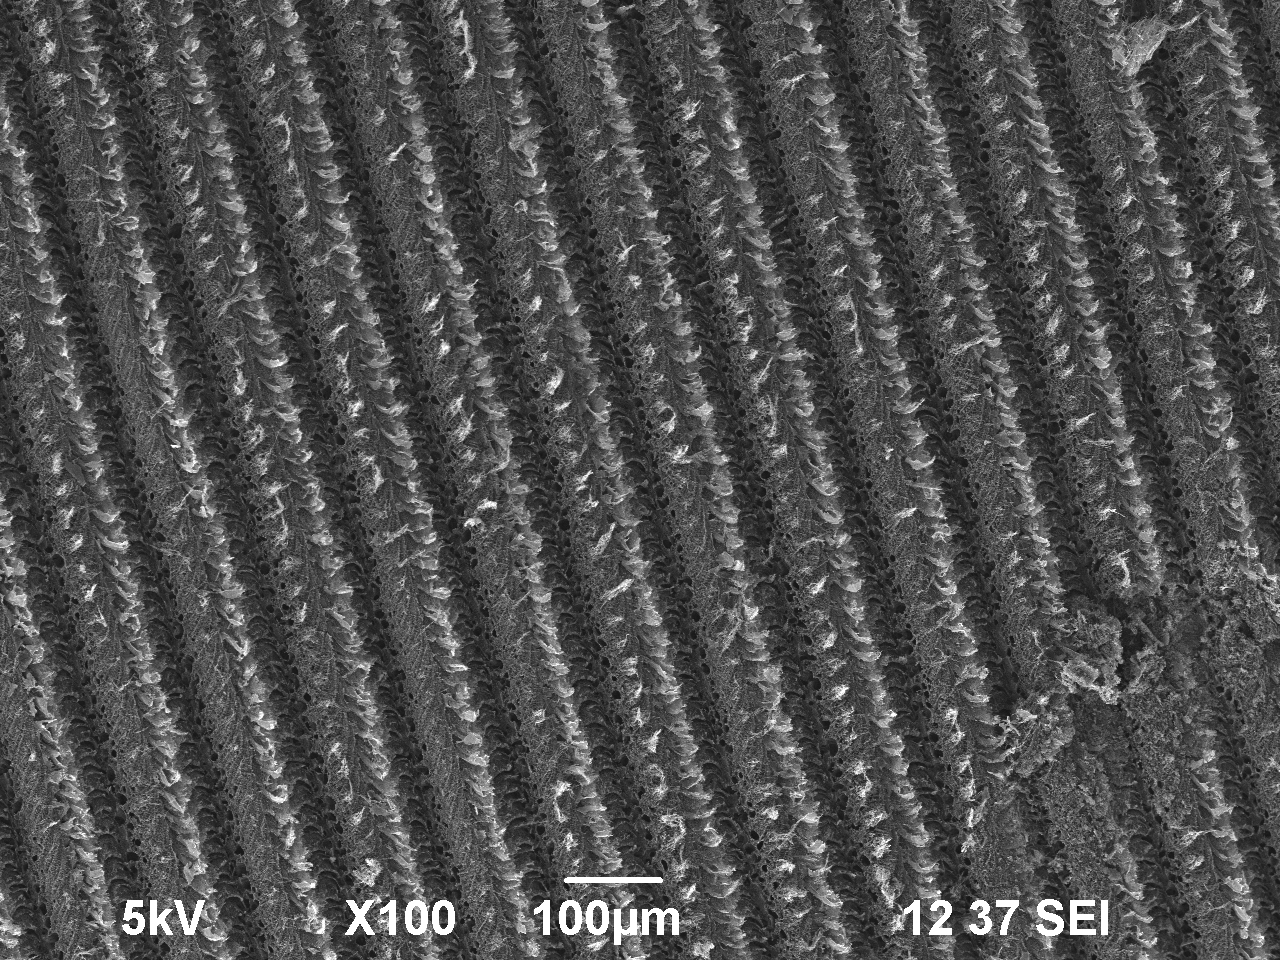
\includegraphics[width=\linewidth]{Figures/Results/SEM/LIGP_PI_1.jpg}
  \caption{LIGP (Laser Power 20$\%$, Speed 10$\%$), X100}
  \label{fig:SEM1}
\end{subfigure}\hfil
\begin{subfigure}{0.49\textwidth}
  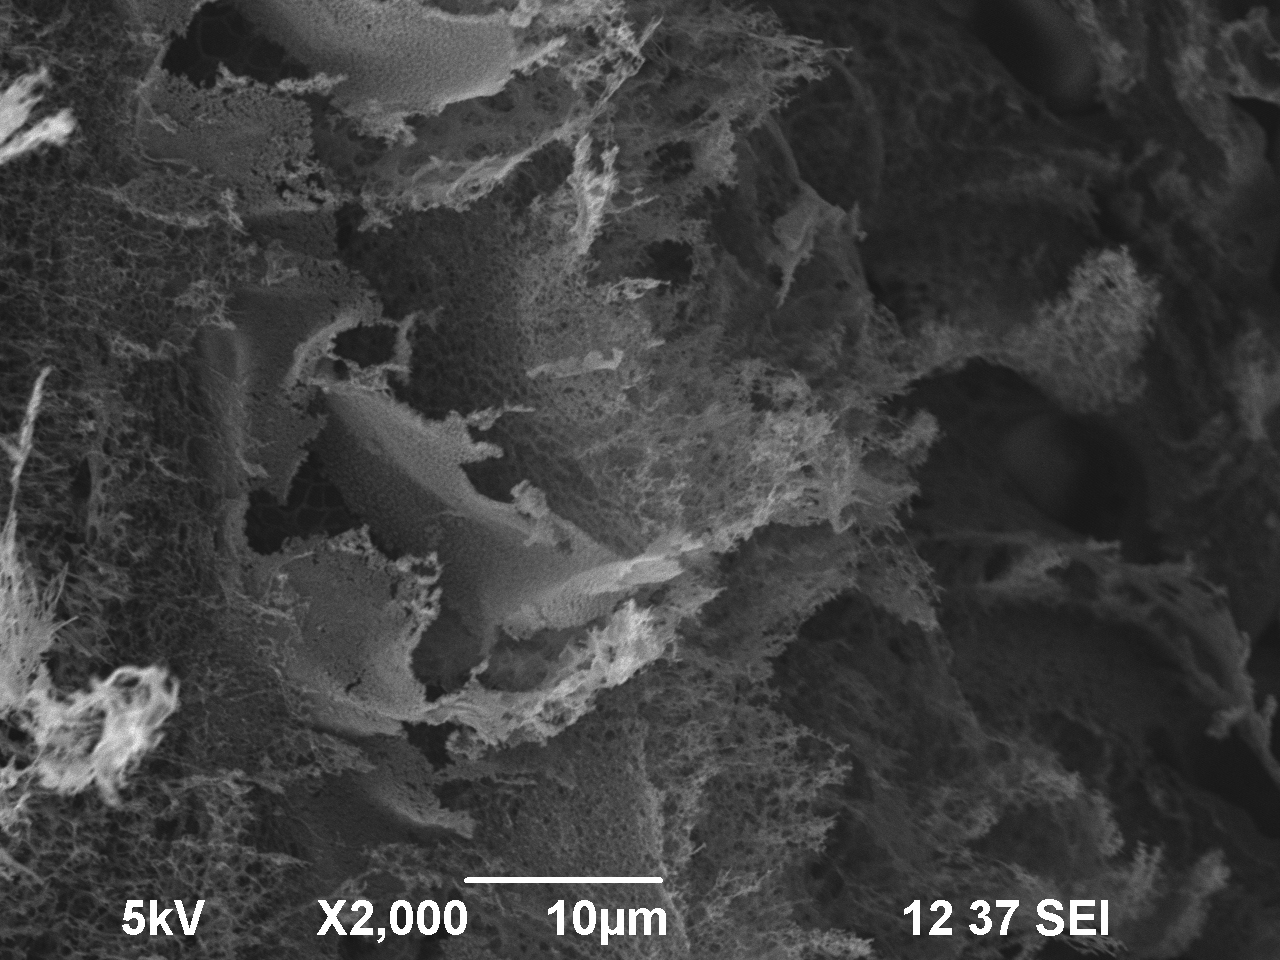
\includegraphics[width=\linewidth]{Figures/Results/SEM/LIGP_PI_2.jpg}
  \caption{LIGP, X2000, Porous Structure of Flakes}
  \label{fig:SEM3}
\end{subfigure}\hfil
\medskip
\begin{subfigure}{0.49\textwidth}
  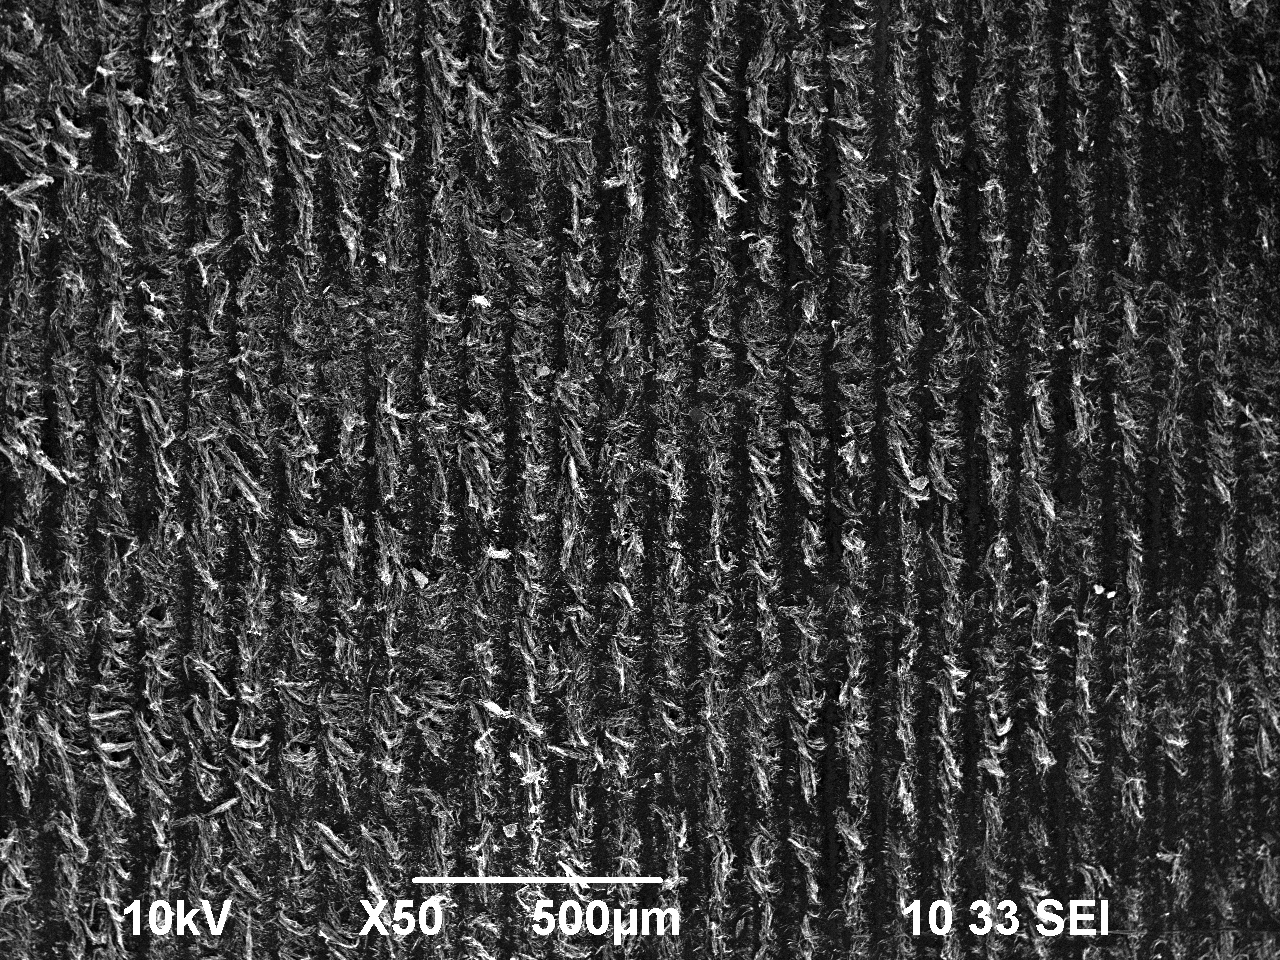
\includegraphics[width=\linewidth]{Figures/Results/SEM/LIGF_1.jpg}
  \caption{LIGF (Laser Power 20$\%$, Speed 10$\%$, X50}
  \label{fig:SEM4}
\end{subfigure}\hfil % <-- added
\begin{subfigure}{0.49\textwidth}
  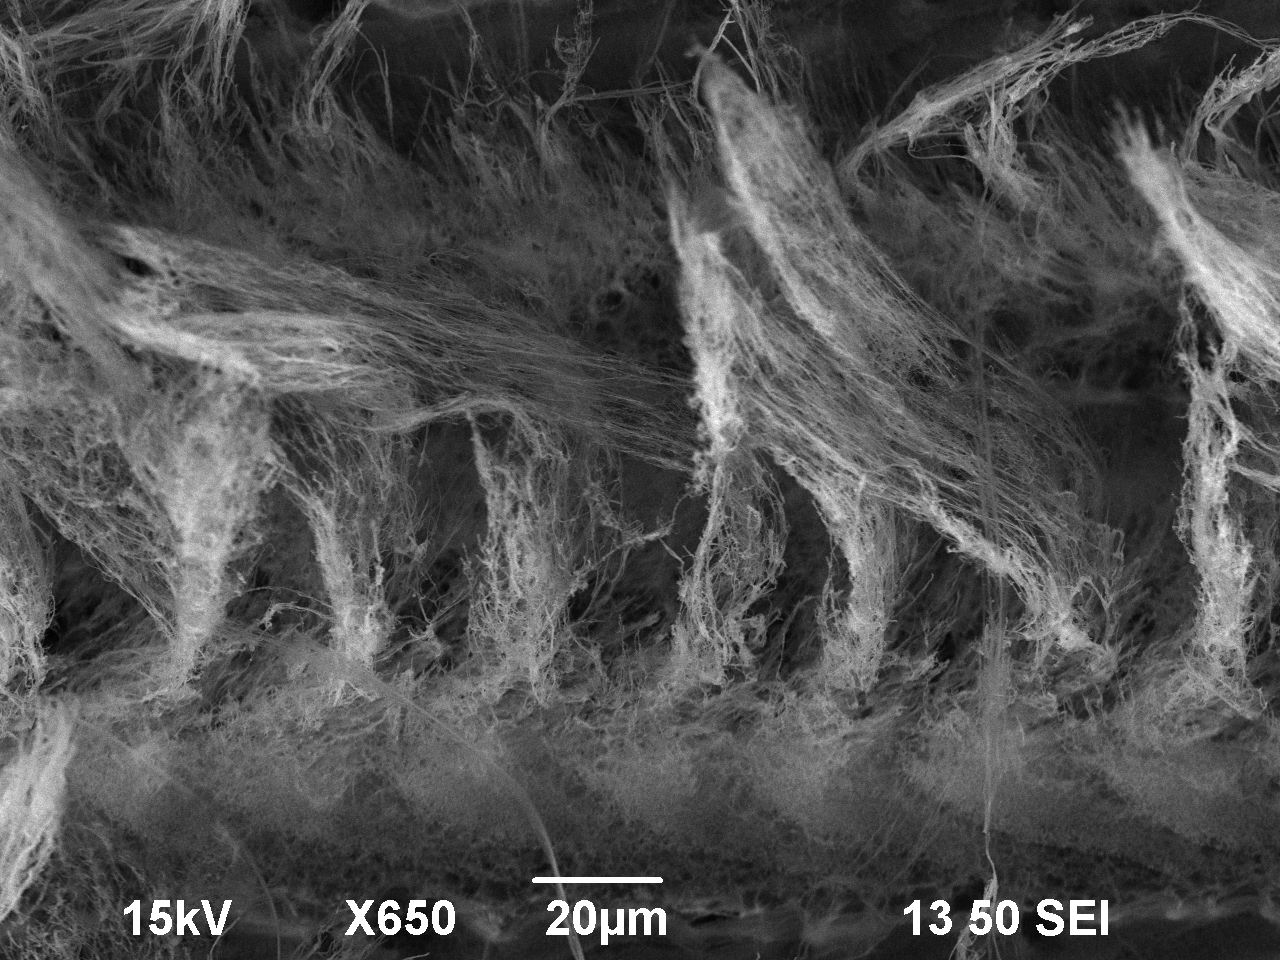
\includegraphics[width=\linewidth]{Figures/Results/SEM/LIG_ID4x650_HANA.jpg}
  \caption{LIGF, X650, Long Fibers \cite{hana}}
  \label{fig:SEM5}
\end{subfigure}\hfil
\caption{SEM images of LIG top surface.}
\label{fig:LIGs-SEMs}
\end{figure}


\subsection{Morphology of Conductive Elastic Biocomposites Based on LIG}

The LIG-PDMS-8:1 composite was obtained by spin coating technique as it was described in the Experimental Setup Section \ref{chapter:Experimental set-up and Results}. The LIG patterns were embedded into PDMS and subsequently peeled off of the original polyimide substrate, which means the originally unseen bottom part of the LIG became the new interface of the composite device. It is worth mentioning that the peeling off process was drastically improved if beforehand the specimen were submerged into EtAc solvent for 5-10 minutes. In some cases the films would then come off themselves without additional pulling force needed. This fact helped to keep the interface area untouched and undamaged. It also helped to ensure that virtually all the LIG was transferred to the LIG-PDMS composite. The interface on the peeled off side was investigated with a help of a light microscope to see if the LIG was fully emerged into the polymeric matrix. It was found that the surface can sustain light scratching without any solitary LIG particles being detached from the surface. Figure \ref{fig:LIG-PDMS-LM} reveals that the alternating line pattern of LIG stays preserved after the transfer.

\begin{figure}[H]
\centering

\includegraphics[width=0.6\textwidth]{Figures/Placeholder.jpg}
\medskip
\captionsetup{width=0.6\linewidth}
\caption{Light microscope picture of the LIGP-PDMS composite surface on the peeled off side.}
\label{fig:LIG-PDMS-LM}
\end{figure}

For the SEM some of the previously mentioned supercapacitor electrodes with VIAs contacts were used, as they came in very useful for avoiding the overcharging effects while imaging. As one sees it in Figure \ref{fig:SEM6} the composite is mainly conductive with solitary islands of non-conductive PDMS which becomes overcharged by the electron beam. Although the specimen in this picture was produced from LIGF, no fibers can be seen as all of them are embedded into the bulk of the composite leaving the macroporous interface areas at the top surface. 

\begin{figure}[H]
\centering
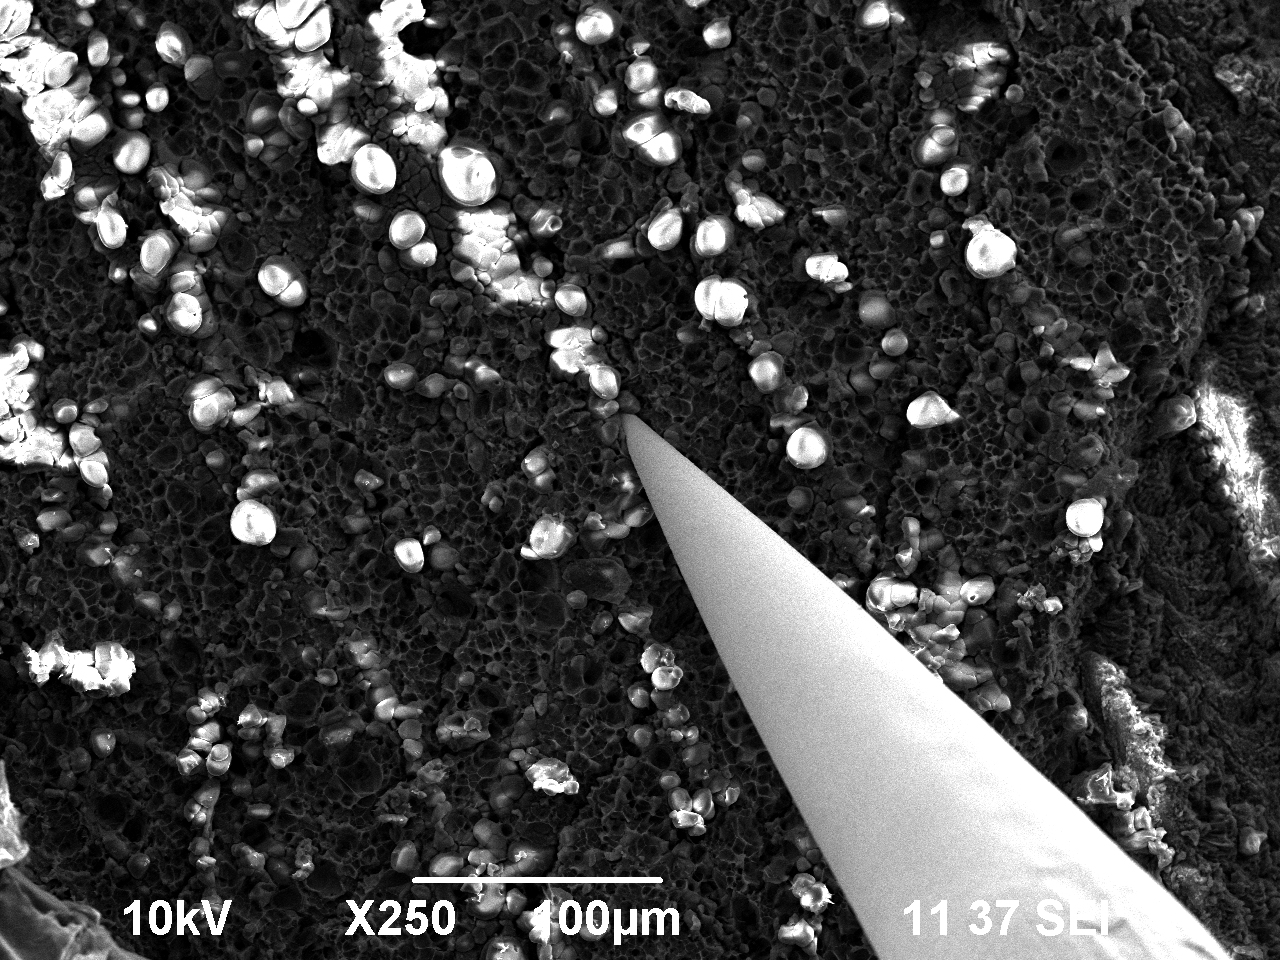
\includegraphics[width=1\textwidth]{Figures/Results/SEM/LIGF_PDMS_1.jpg}
\medskip
\captionsetup{width=0.7\linewidth}
\caption{SEM image of LIGF layer embedded into PDMS and peeled off from the original PI substrate. }
\label{fig:SEM6}
\end{figure}


----------------

PU + LIG 

LM pictures, SEM ideally


\subsection{Morphological Characterization of LIGs with AFM}

----------------

\subsection{Mass Density Characterization of LIGs}

The summary of the obtained mass density values of LIGs supported by various substrates can be seen in the following Table \ref{tab:LIG_mass} 
\begin{table}[H]
\centering
    \caption{Mass per Surface Area of LIGs on Various Substrates}
    \label{tab:LIG_mass} 
\medskip
\medskip
\centering
\begin{tabular}{ l | l | l  } 

LIG Type & Substrate Material & \pbox{100px}{LIG 2D Mass Density\\ $\pm$ Error [$mg/cm^2$]}\\[15px]
\hline
LIGP & Kapton$^{TM}$ Film/Tape 50 $\mu$m & 0.20 $\pm$ 0.01 \\ [13px]
LIGF & Kapton$^{TM}$ Film/Tape 50 $\mu$m & 0.51 $\pm$ 0.04\\ [13px]
LIGP & PEEK Film 100 $\mu$m & ? \\ [13px]
LIGP & PDMS-8:1 & 0.20 $\pm$ 0.01 \\ [13px]
LIGF & PDMS-8:1 & 0.51 $\pm$ 0.04\\ [13px]
LIGP & MPU & 0.11 $\pm$ 0.01 \\ [13px]
LIGF & MPU & 0.28 $\pm$ 0.06\\ [13px]
\end{tabular}
\end{table}

\subsection{Thickness Measurements}

The thickness of commercially available Kapton$^{TM}$ film and tape was measured by profilometry technique and was estimated to be $50\pm0.5\:\mu m$, which was in compliance with the tolerance values claimed by the manufacturer.

The thickness of LIG-PDMS-8:1 composites was estimated by the light microscope technique which was previously described in Experimental Setup Section \ref{chapter:Experimental set-up and Results}. As one can see in the following Figures \ref{fig:PDMS-81-double-layer} and \ref{fig:LIGF-PDMS-cross-section} the thickness of the bare PDMS-8:1 (double layered) was found to be $\approx70-80\:\mu m$. The thickness of the composite part was estimated to be $\sim 350-450\:\mu m$. In the picture on the right, the fully embedded long fibers of LIGF can be seen. 

\begin{figure}[H]
\begin{subfigure}{0.49\textwidth}
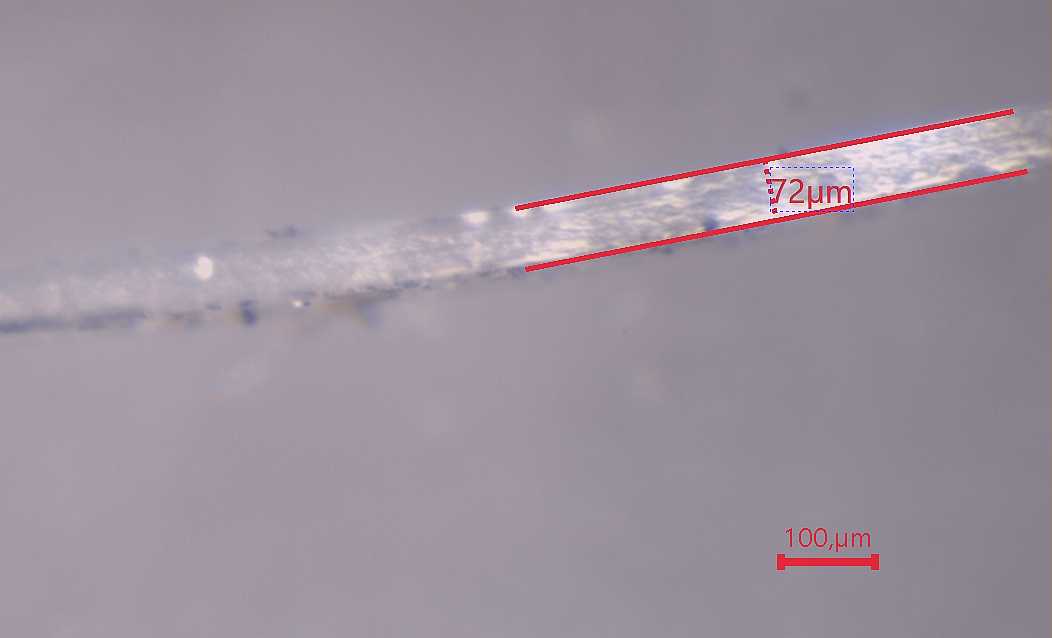
\includegraphics[width=0.95\textwidth]{Figures/Results/PDMS-1-layer-10-1-CS2.jpg} 
\captionsetup{width=0.9\linewidth}
\caption{Bare PDMS-8:1 layer}
\label{fig:PDMS-81-double-layer}
\end{subfigure}
\begin{subfigure}{0.49\textwidth}
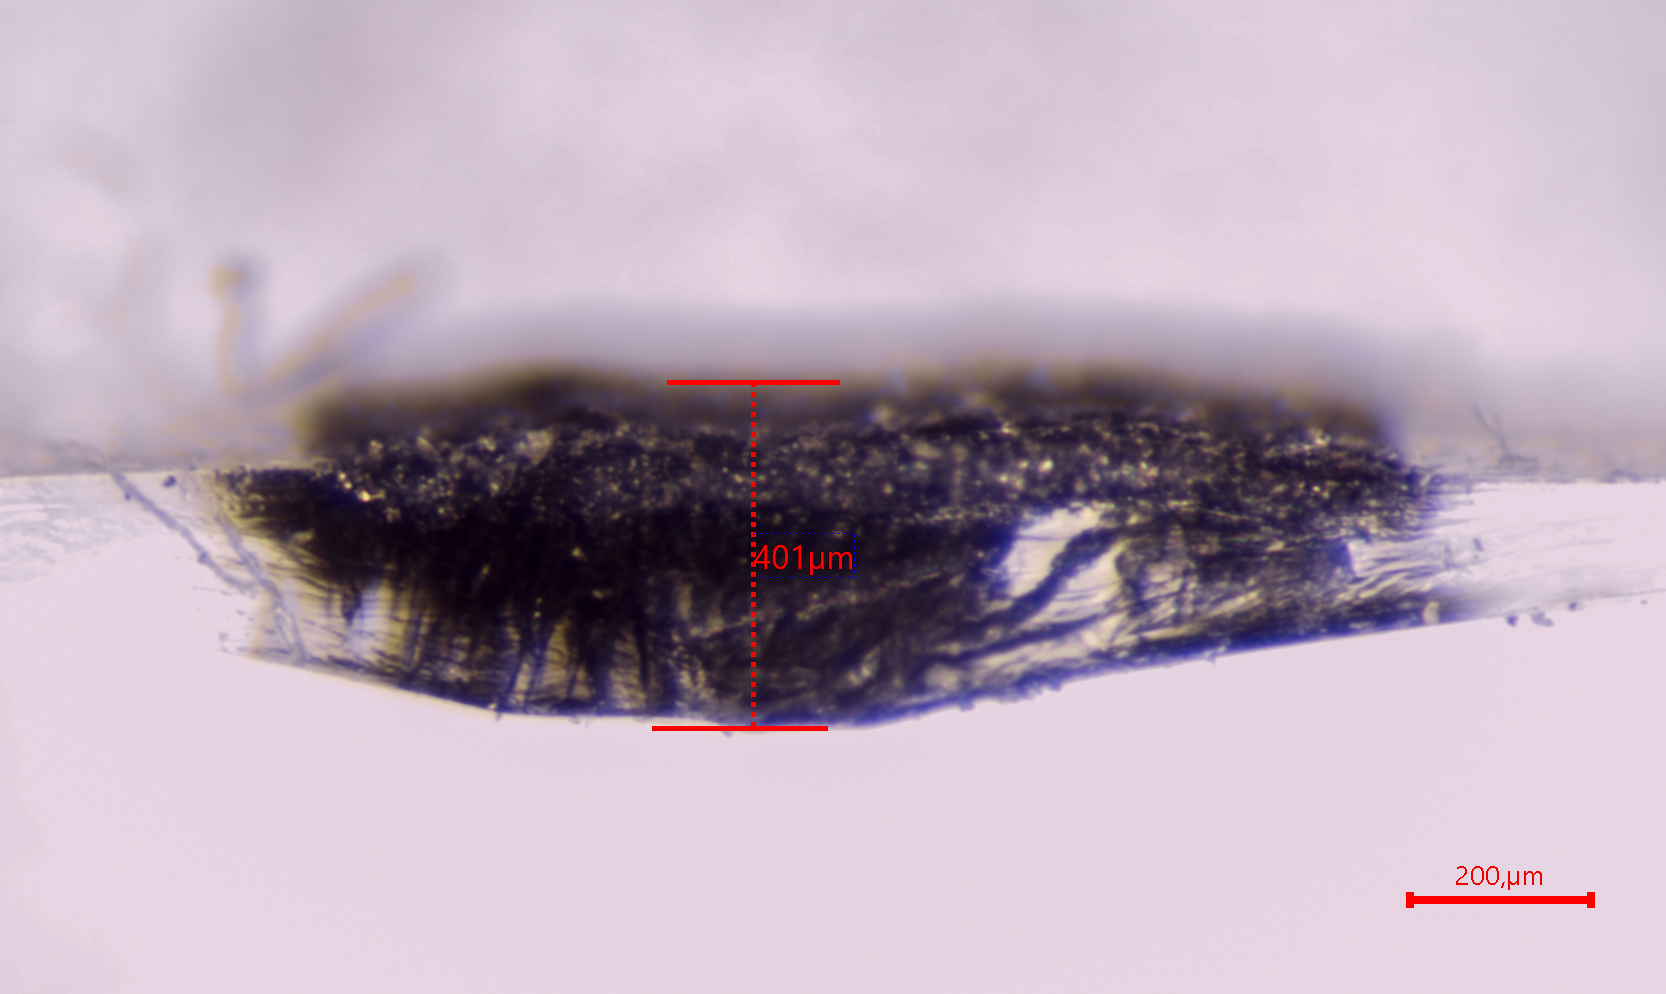
\includegraphics[width=0.95\textwidth]{Figures/Results/LIG-Fiber-in-PDMS-1-layer-10-1-CS1.jpg}
\captionsetup{width=0.9\linewidth}
\caption{LIGF-PDMS-8:1 cross-section. }
\label{fig:LIGF-PDMS-cross-section}
\end{subfigure}
\medskip
\caption{Thickness evaluation of LIGF-PDMS-8:1 composite}
\label{fig:LIGP_BET}
\end{figure}

The thickness of the LIGP-PDMS-8:1 composite part was estimated to be in a range $\sim 250-350\:\mu m$.     


\subsection{Electromechanical Characterization of Composites}
Elasticity and Resistivity of PDMS, PDMS+LIG, PU, PU+LIG vs strain \& humidity rate.

The alternating line pattern of LIG which staid preserved also after the transfer to PDMS or MPU. Therefore the specimen with the parallel and perpendicular direction of scribbed lines in respect to the stretching direction were investigated.

graph 1: E vs F at T = 25$\degree$C for PDMS
graph 2: E vs F at T = 25$\degree$C for PDMS + LIGP/LIGF parallel
graph 3: E vs F at T = 25$\degree$C for PDMS + LIGP/LIGF perpendicular

graph 4: F vs HR\% for PDMS
graph 5: F vs HR\% for PDMS + LIGP/LIGF parallel
graph 6: F vs HR\% for PDMS + LIGP/LIGF perpendicular

graph 7: E vs F at T = 25$\degree$C for FM
graph 8: E vs F at T = 25$\degree$C for FM + LIGP/LIGF parallel/perpendicular



\section{Surface Area and Porosity Characterization}

\subsection{Gas Adsorption Measurements (BET) for Powder LIGs}

The surface area and porosity values obtained for LIGP and LIGF powders via adsorption isotherms are shown in the Table \ref{tab:powder_BET_results}. For the LIGF material the results of the sample LIGF (2) were taken as the final value because its adsorption isotherm was obtained for the full range of relative pressure, as will be described later in this subsection.

\begin{table}[H]
\centering
    \caption{Powder BET Measurements Results}
    \label{tab:powder_BET_results} 
\medskip
\medskip
\begin{tabular}{ l | l | l | l | l | l } 

LIG Sample &  $C_{BET}$ & $n_m\:[cm^3/g]$ & $A_{BET}\:[m^2/g]$ & TPV $[cm^3/g]$ & TPSA\footnotemark[1]  $[m^2/g]$\\[15px]
\hline

LIGP     & 488.9 & 44.01 & 192 $\displaystyle \pm$ 1 &  0.26215 & 98.9 \\[15px]

LIGF (2) & 15.8 & 62.15 & 270 $\displaystyle \pm$ 1  & 0.38820 & 146.4  \\[15px]


\end{tabular}
\end{table}

\footnotetext[1]{TPSA - Total pore surface area} 

Figures \ref{fig:LIGP_BET_Ads_Des} and \ref{fig:LIGF_BET_Ads_Des} represent the adsorption and desorption isotherms for LIGP and LIGF. The isotherms correspond to the Type II by the IUPAC classification. No significant hysteresis can be seen for the both types of LIG, which indicates an absence of mesoporosity in the bulk. As it can be seen in the Figures \ref{fig:LIGP_BET_plot} and \ref{fig:LIGF_BET_plot} the slope value of the linear part of the isotherm $s$ is lower for the LIGF material which leads to a significantly lower value of $C_{BET}$ in BET analysis. 

\begin{figure}[H]
\begin{subfigure}{0.51\textwidth}
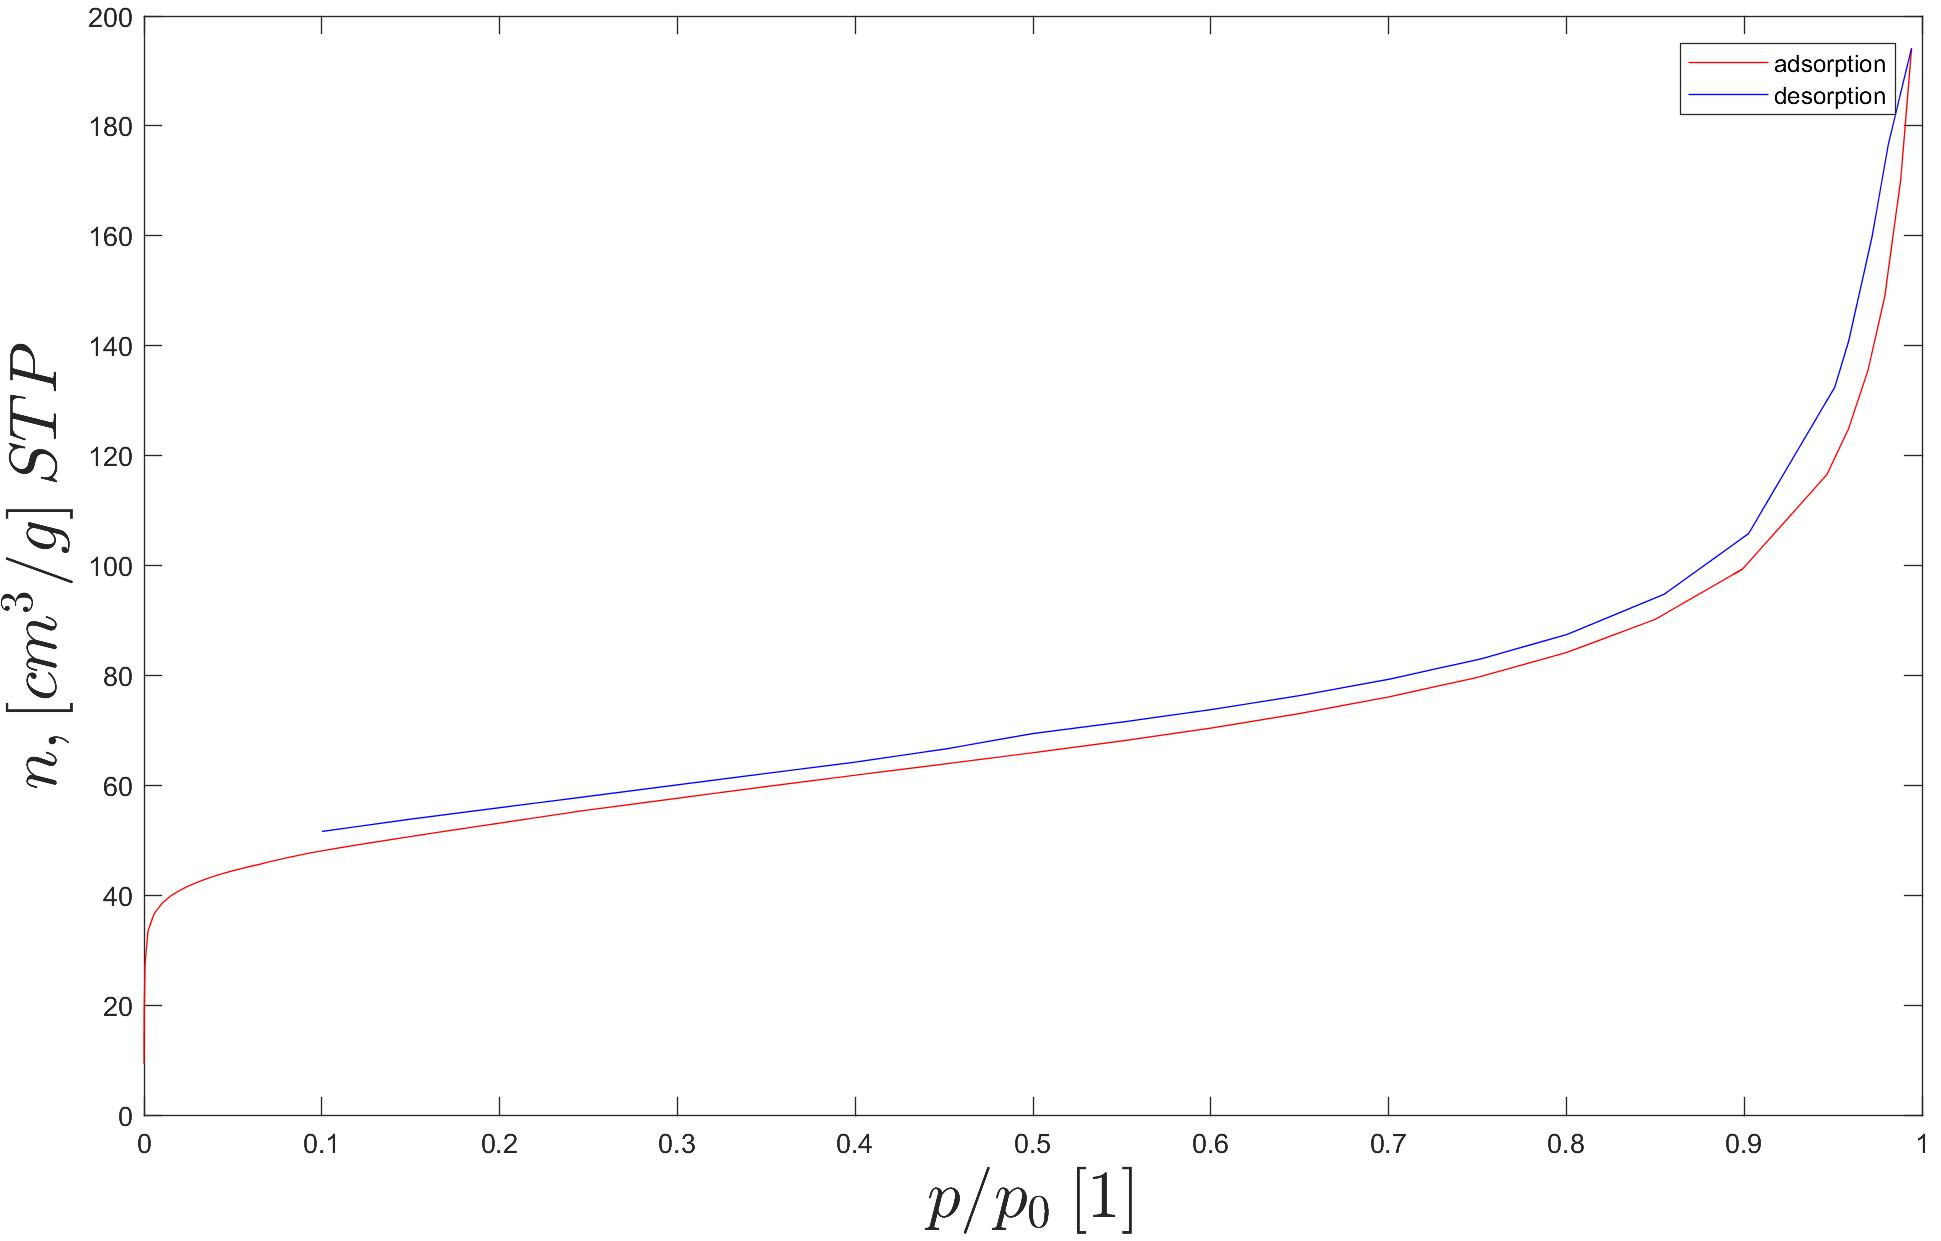
\includegraphics[width=0.95\textwidth]{Figures/Results/LIGP_Adsorption_Desorption_Isotherm.jpg} 
\captionsetup{width=0.9\linewidth}
\caption{Adsorption/Desorption Isotherm for LIGP}
\label{fig:LIGP_BET_Ads_Des}
\end{subfigure}
\begin{subfigure}{0.48\textwidth}
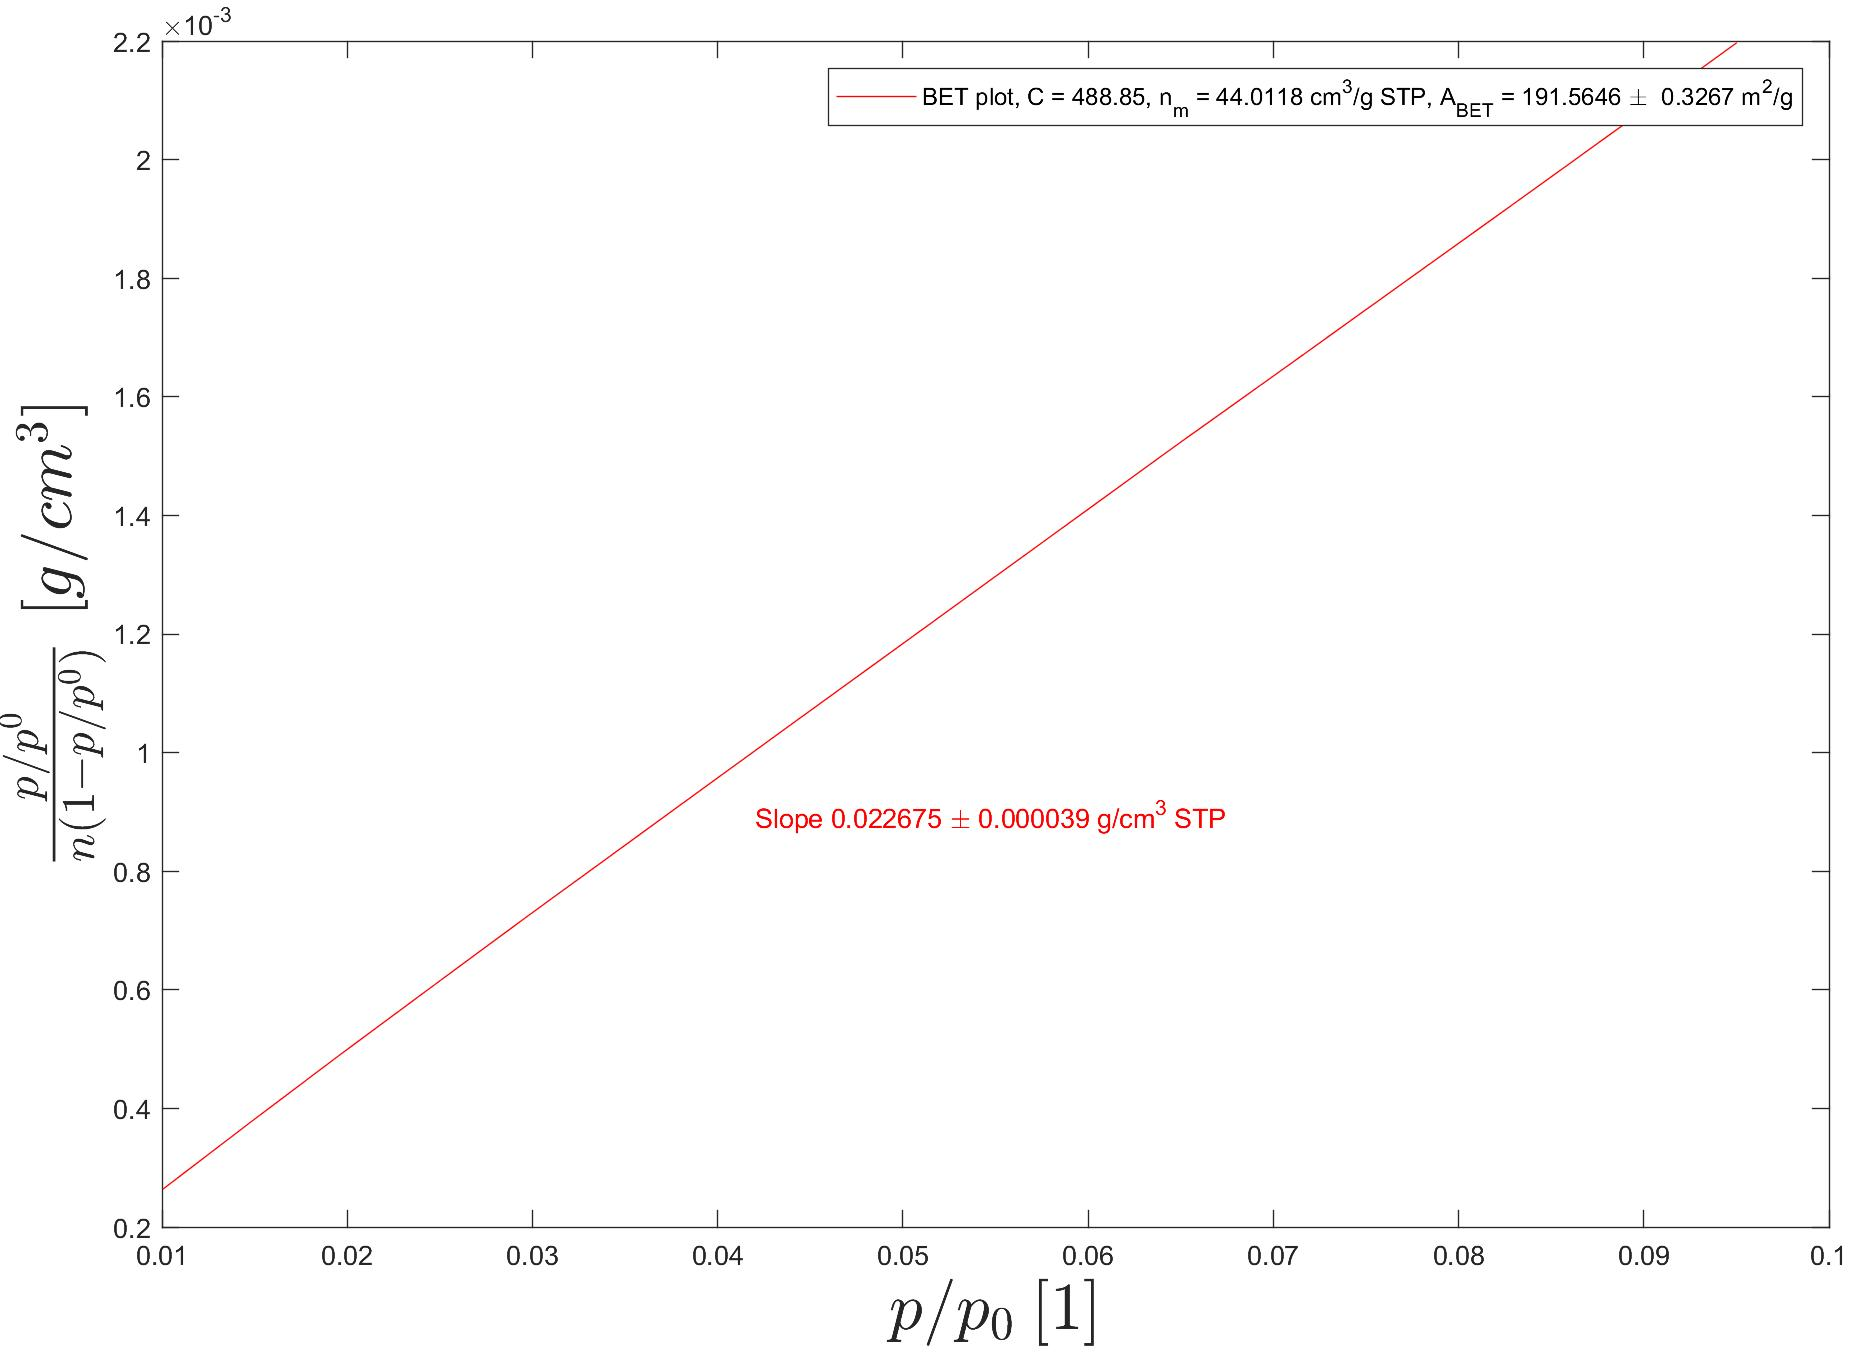
\includegraphics[width=0.95\textwidth]{Figures/Results/LIGP_BET_plot.jpg}
\captionsetup{width=0.9\linewidth}
\caption{Linear BET plot for $p/p^0$ 0.01 to 0.1}
\label{fig:LIGP_BET_plot}
\end{subfigure}
\medskip
\caption{Adsorption data for LIGP BET analysis}
\label{fig:LIGP_BET-2}
\end{figure}



\begin{figure}[H]
\begin{subfigure}{0.51\textwidth}
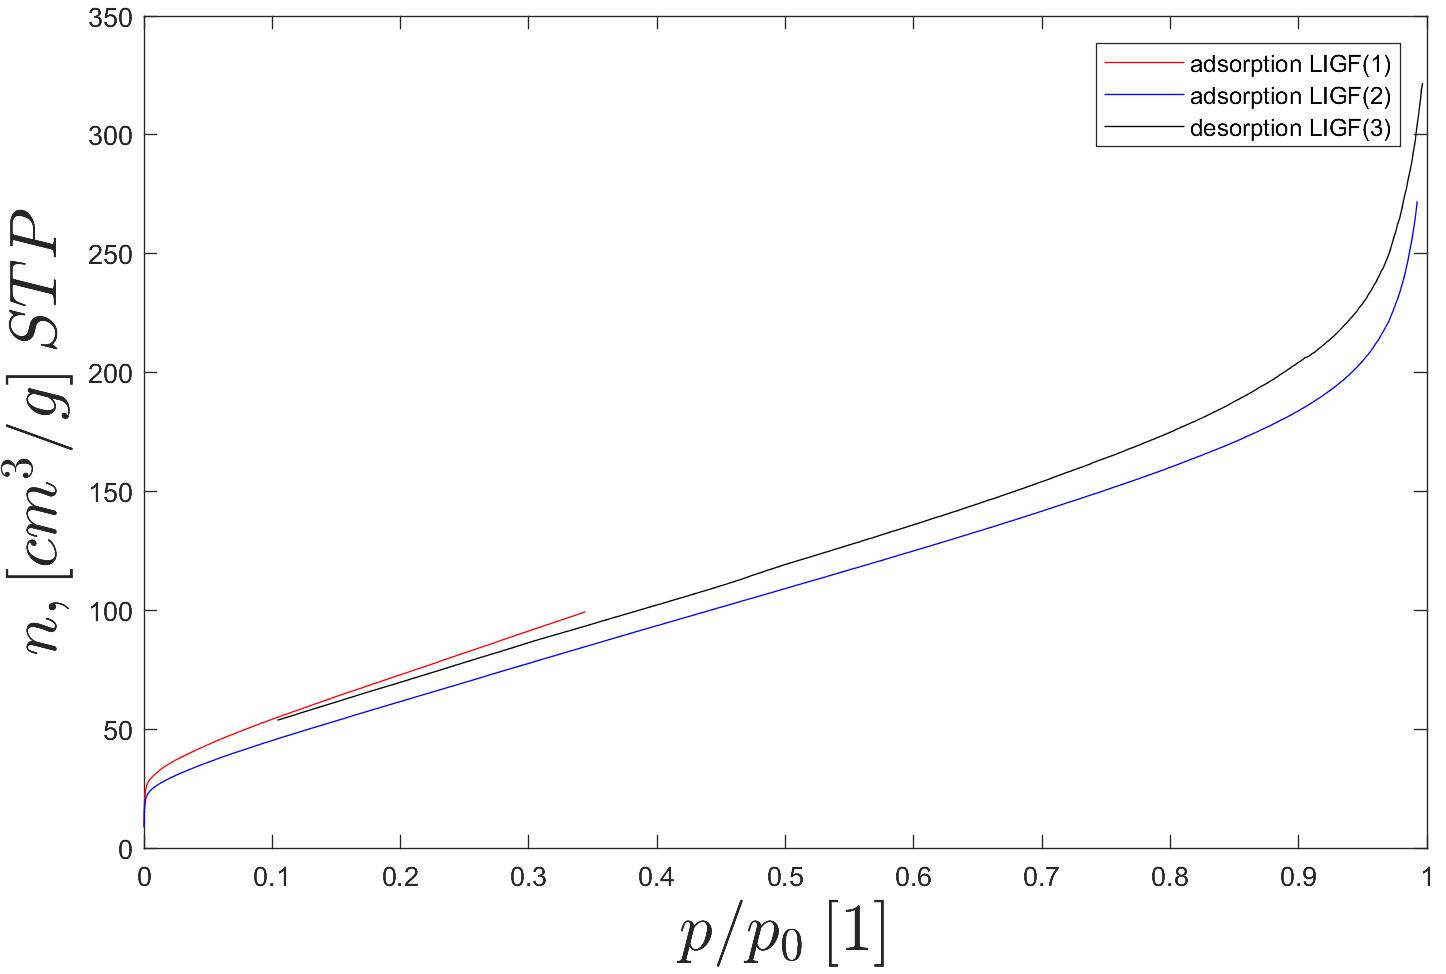
\includegraphics[width=0.95\textwidth]{Figures/Results/LIGF_Adsorption_Desorption_Isotherms.jpg} 
\captionsetup{width=0.9\linewidth}
\caption{Adsorption/Desorption Isotherm for LIGF}
\label{fig:LIGF_BET_Ads_Des}
\end{subfigure}
\begin{subfigure}{0.48\textwidth}
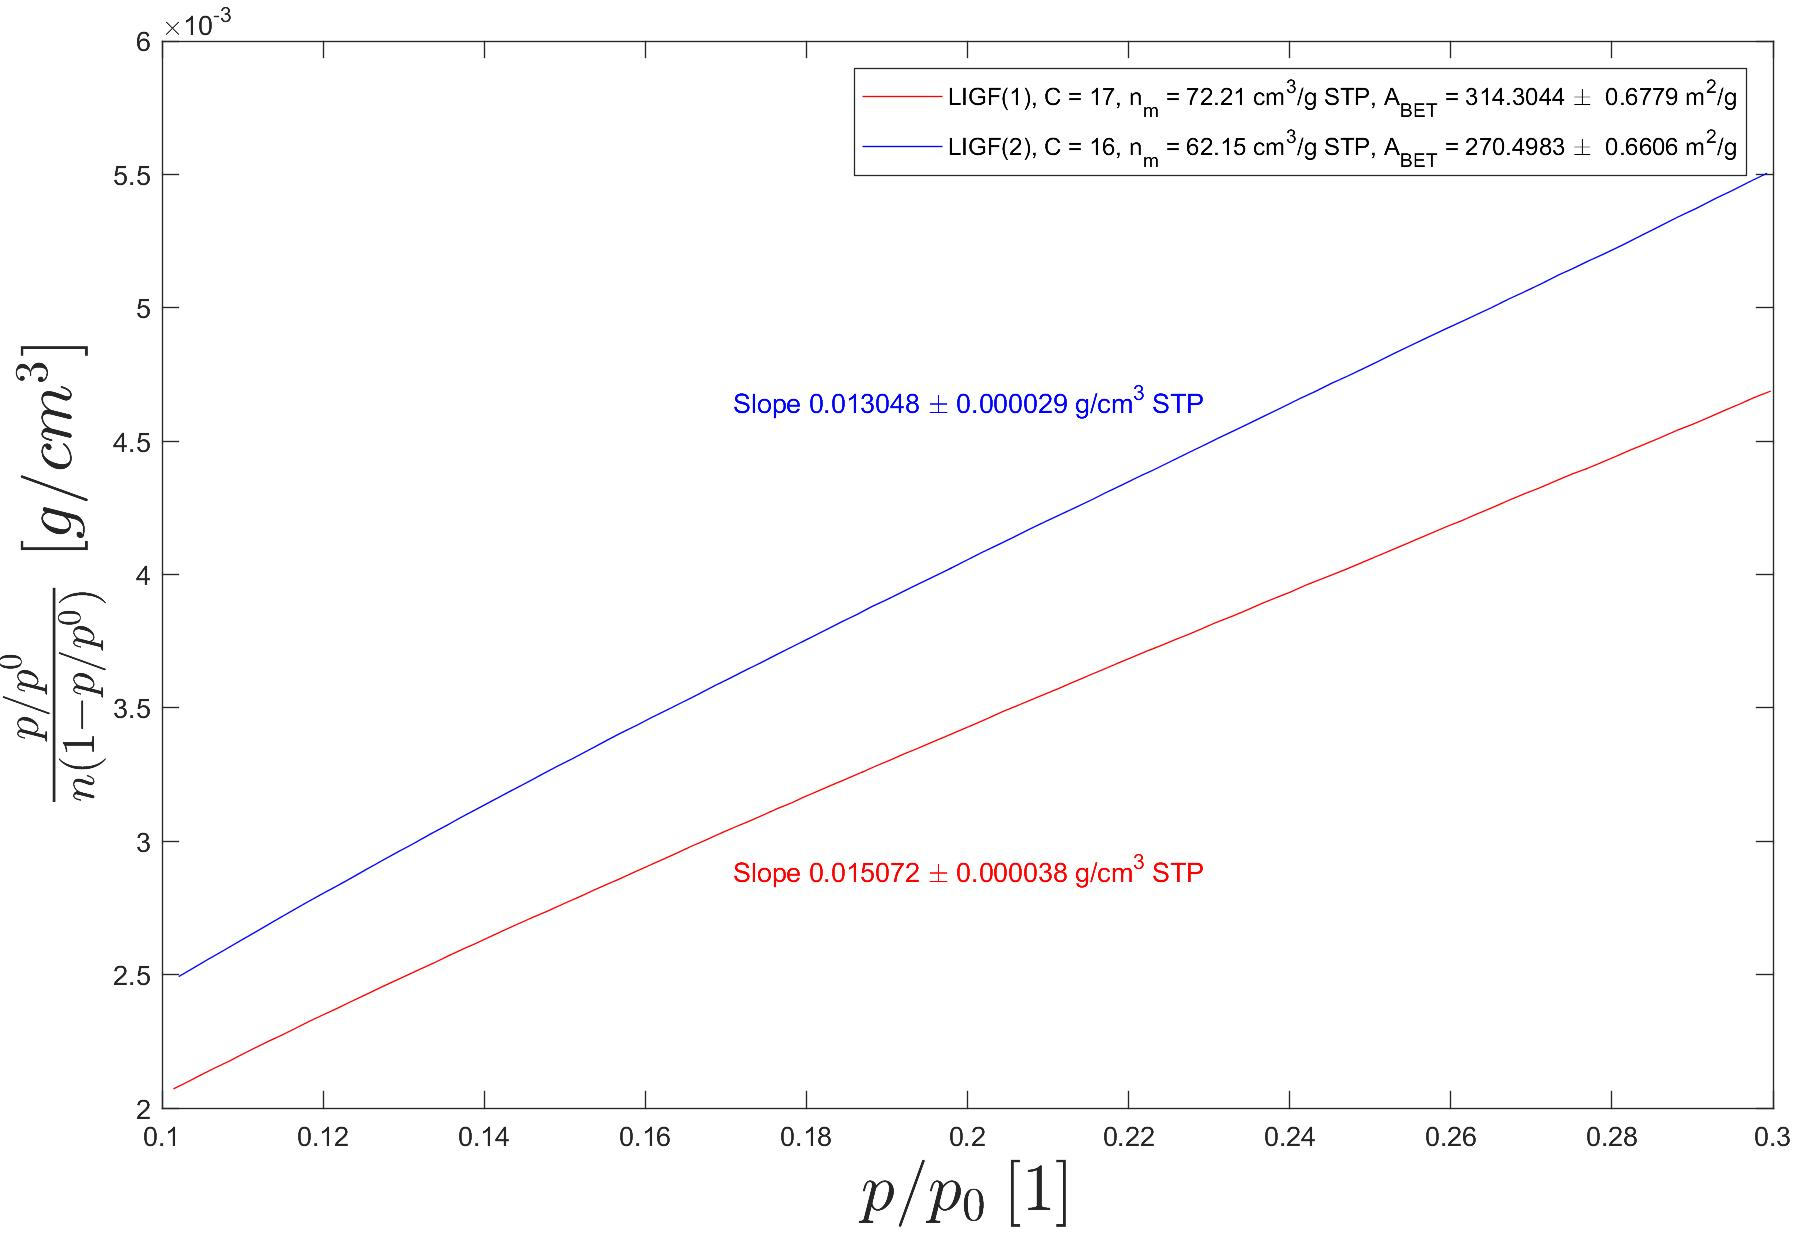
\includegraphics[width=0.95\textwidth]{Figures/Results/LIGF_BET_plots.jpg}
\captionsetup{width=0.9\linewidth}
\caption{Linear BET plot for $p/p^0$ 0.1 to 0.3}
\label{fig:LIGF_BET_plot}
\end{subfigure}
\medskip
\caption{Adsorption data for LIGF BET analysis}
\label{fig:LIGF_BET}
\end{figure}


As mentioned in Section \ref{chapter:Theory}, the BET method can be applied to  Type II and Type IV isotherms, but extreme caution is needed in the presence of micropores (i.e., with Type I isotherms and combinations of Types I and II or Types I and IV isotherms) \cite{thommes_physisorption_2015}. The pore size and pore volume evaluations were performed via N2 $@$ 77 on Carbon Slit Pores by NLDFT model \cite{NLDFT} and have shown the investigated LIG materials were strictly microporous as presented by the differential pore volume distributions in Figure \ref{fig:diff_volume_vs_pore_width}. As can be seen from the graphs, the porosity of the LIGP can be accounted to the micropores ranging from 7 to 15 $\AA$ in size, while the bulk of the LIGF is mostly occupied by the pores from 13 to 31 $\AA$ in diameter. 

\begin{figure}[H]
\centering
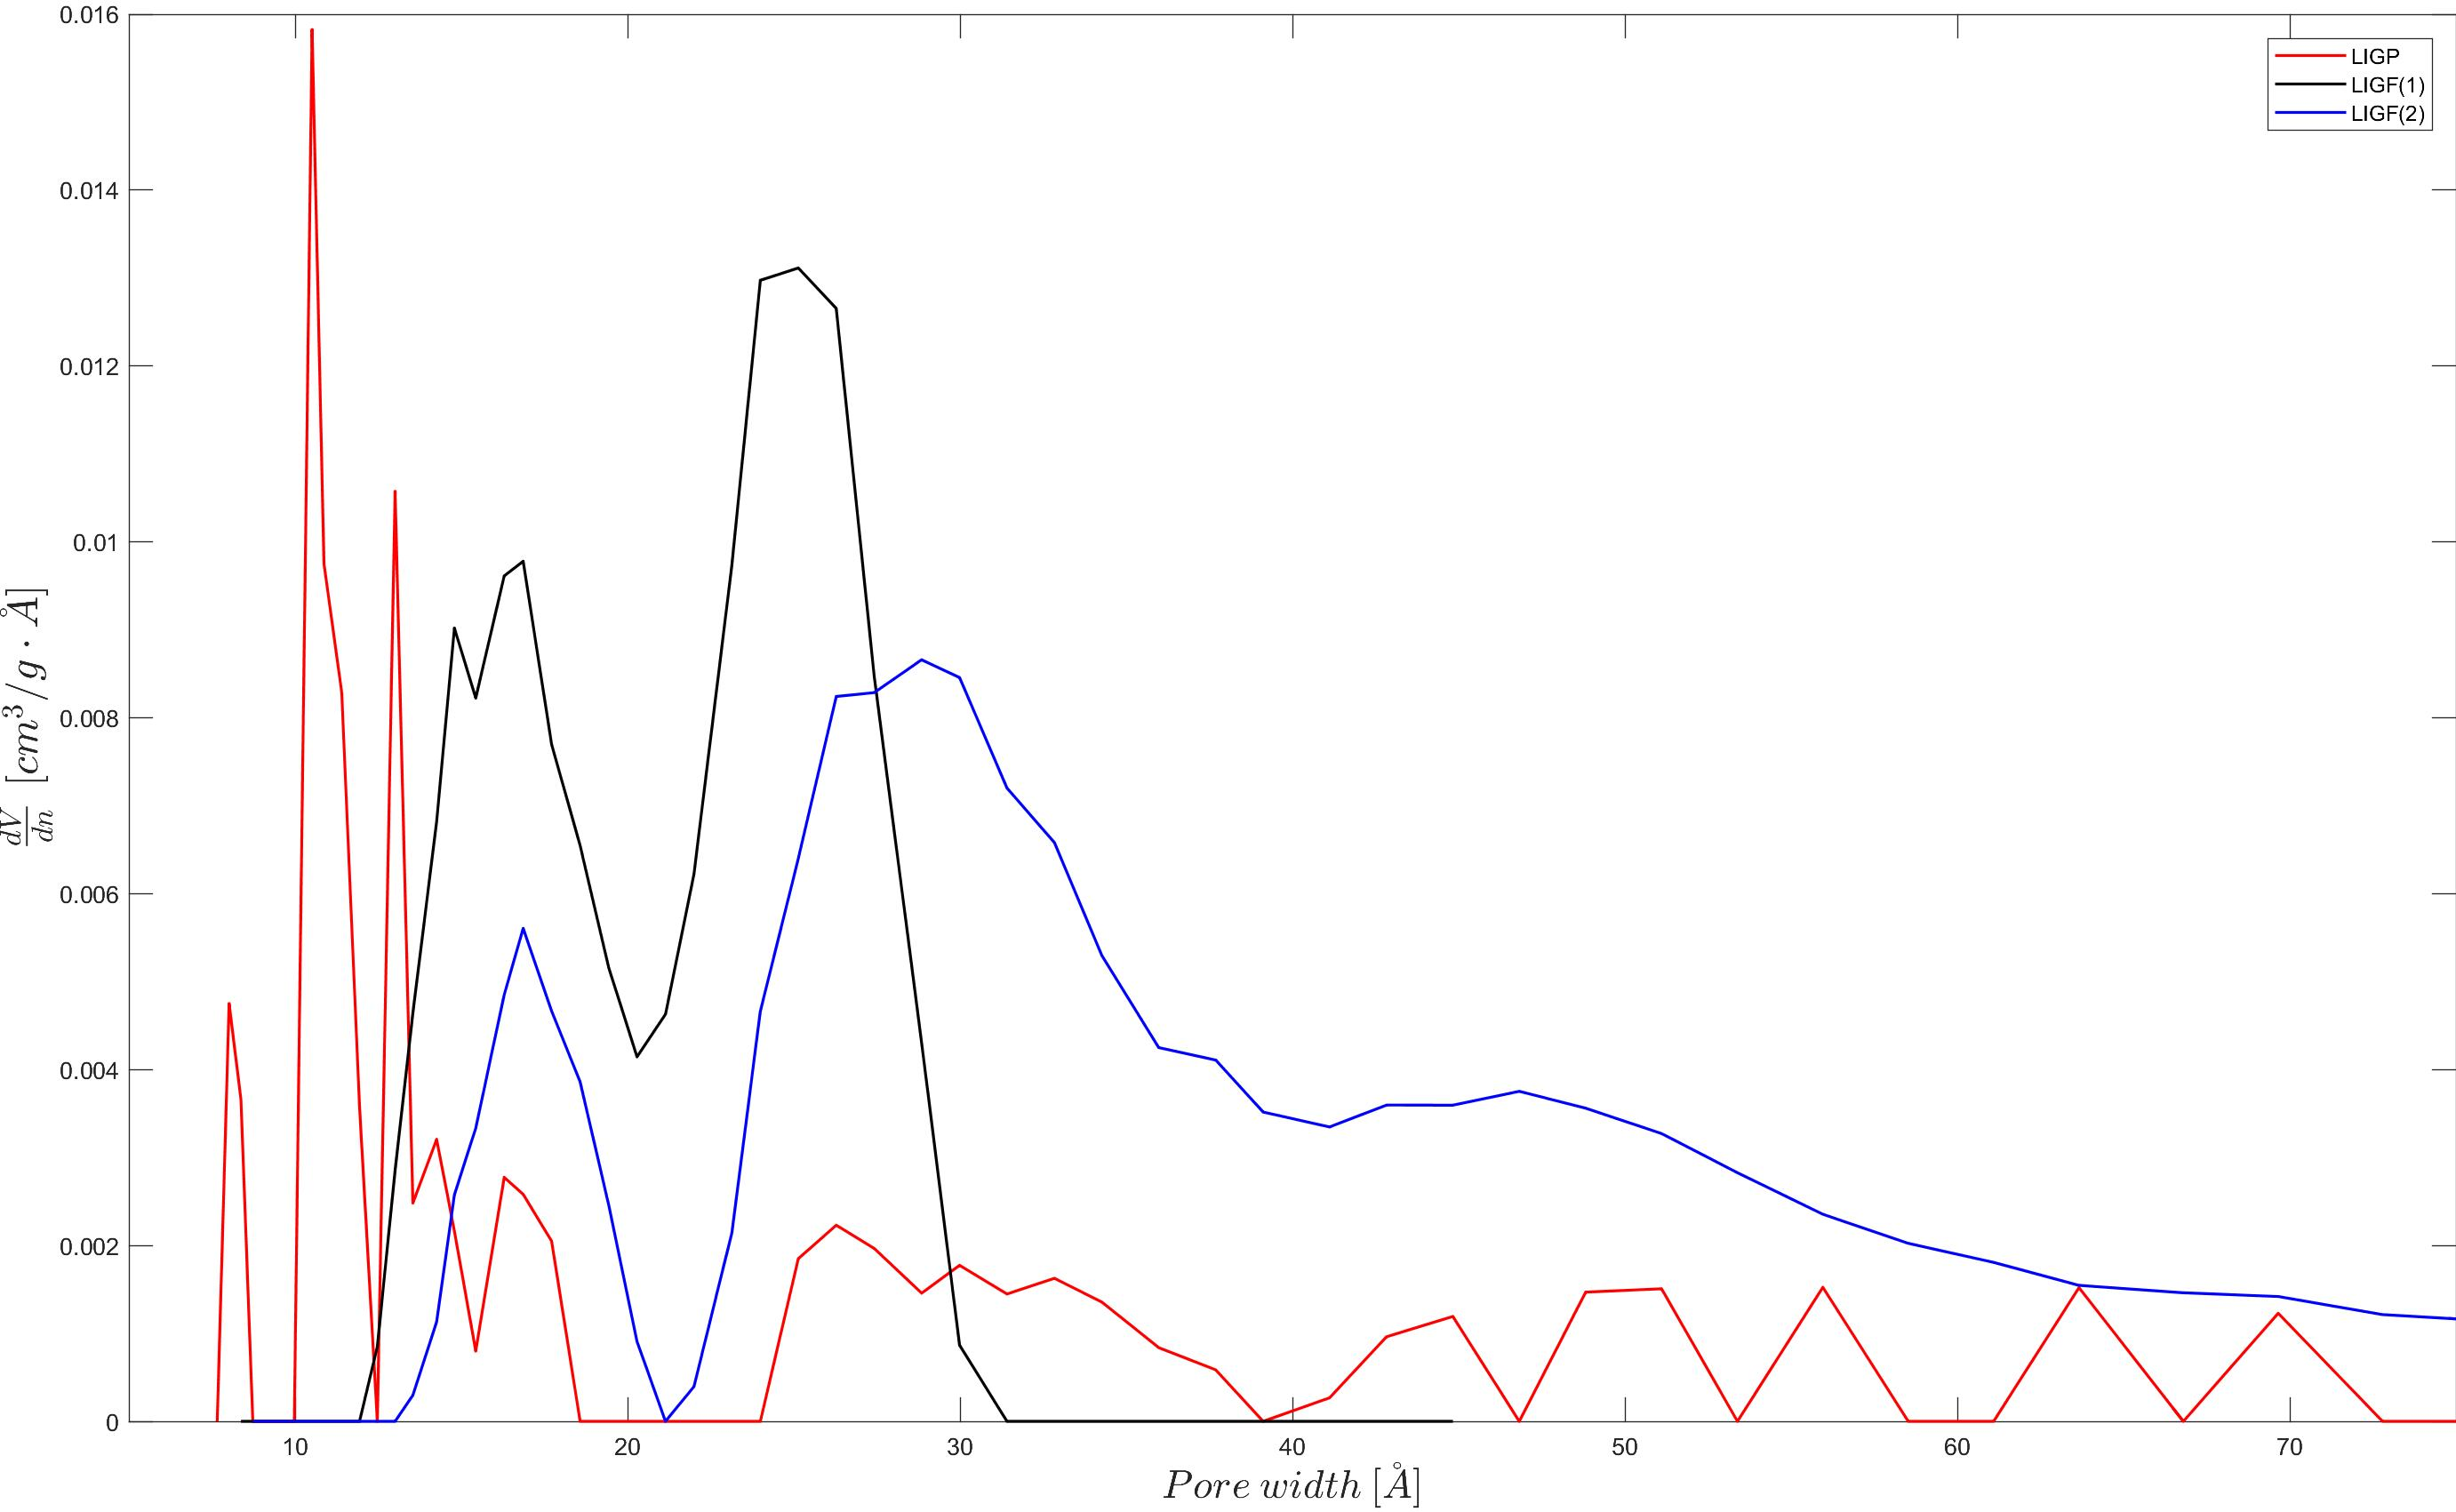
\includegraphics[width=0.6\textwidth]{Figures/Results/Diff_pore_volume_vs_width.jpg}
\medskip
\caption{Differential pore size distributions for LIGP and LIGF}
\label{fig:diff_volume_vs_pore_width}
\end{figure}

Further as visually shown in Figure \ref{fig:cumulative_vs_pore_width}, the total pore volume (TPV), as well as the total pore surface area (TPSA), per unit mass is 48$\%$ larger in the LIGF than in the LIGP. 


\begin{figure}[H]
\centering
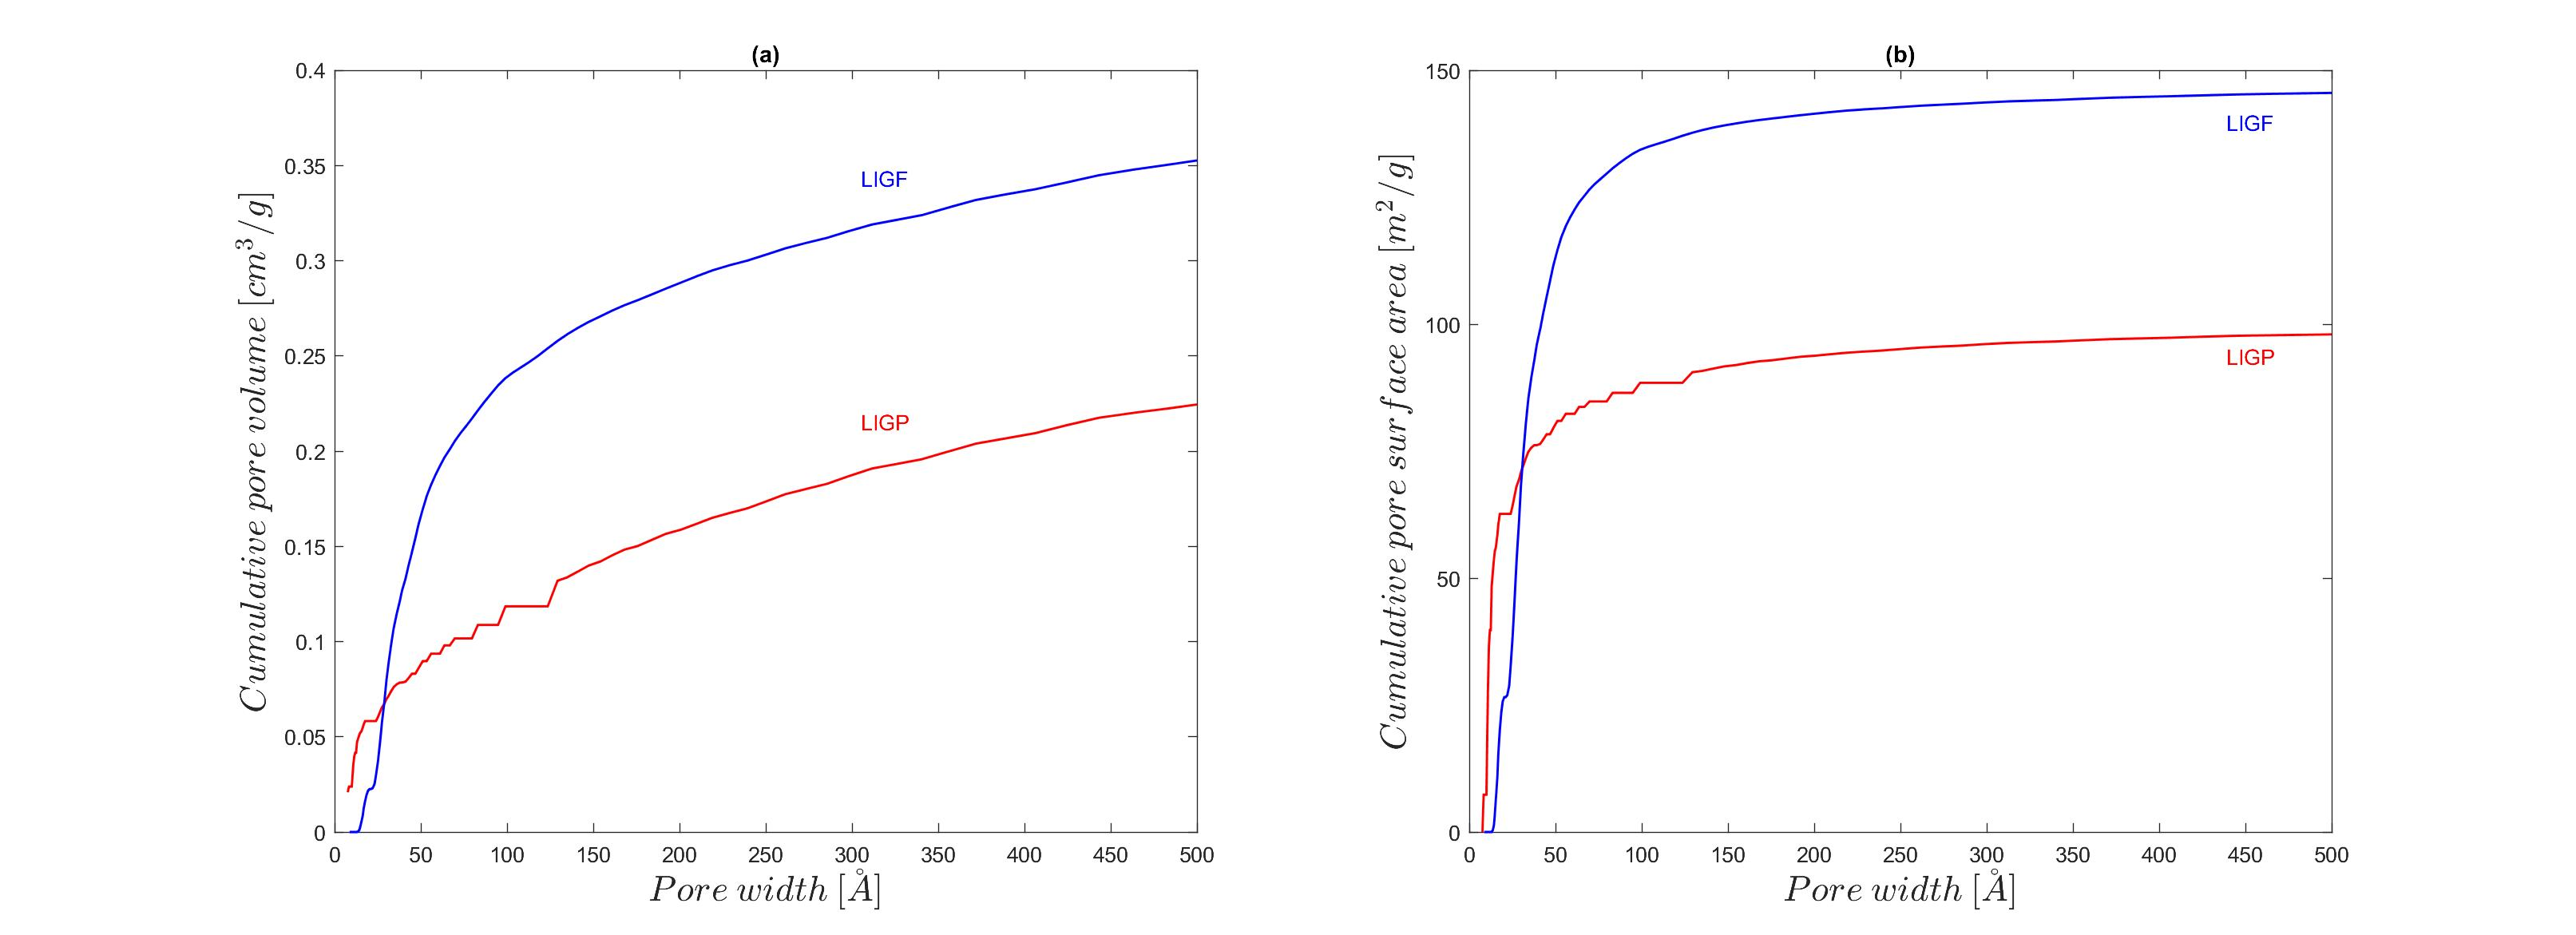
\includegraphics[width=1\textwidth]{Figures/Results/Cumulative_Pore_vol_surf_width.jpg}
\medskip
\captionsetup{width=0.7\linewidth}
\caption{Cumulative Pore volume (a) and Surface area (b) vs. Pore width for LIGP and LIGF(2)}
\label{fig:cumulative_vs_pore_width}
\end{figure}


Comparing our results to the results of Lin $et\ al.$ \cite{lin_laser-induced_2014} as described in Section \ref{chapter:Theory} allows a conclusion that the LIGP and LIGF materials belong to microporous bulk type with much smaller pores as in the LIG material used by Lin. The values of the BET specific surface area obtained in this study are lower than those provided by Lin $et\:al.$ ($\sim 342m^2/g$), but belong to the mutual range of $200\sim350\:m^2/g$.

XXX???Consider to discuss that the surface area and the pore volume determined by using the various empirical models are approximated values. Also what about Type II which is for non-porous vs. the result with the micropores?

\subsection{Gas Adsorption Analysis of LIG via Gemini$^{TM}$ Technique}

.
.
.

\newpage
\section{LIG Based Supercapacitors}


\subsection{LIG Based Supercapacitor Cells}



The Table \ref{tab:supercapacitor_electrodes} summarizes the list of the LIG based electrodes prepared for the subsequent electrochemical analysis.

\begin{table}[H]
\centering
    \caption{The List of LIG Based Electrodes}
    \label{tab:supercapacitor_electrodes} 
\medskip
\medskip
\begin{tabular}{ l | l | l | l | l| l  } 


	\pbox{100px}{Electrode\\Type $\#$} & LIG Type\footnotemark[1] & Substrate Material & Cell Type & Electrolyte & \pbox{100px}{N of pairs\\prepared/tested} \\ [13px]\hline
	1  & LIGP & Kapton$^{TM}$ Film 50 $\mu$m & Swagelok$^{TM}$& $NaNO_3\:1M$ & 5/2 \\ [13px]
	2  & LIGF & Kapton$^{TM}$ Film 50 $\mu$m & Swagelok$^{TM}$& $NaNO_3\:1M$ & 3/1\\ [13px]
	
	3  & LIGF & PDMS-8:1 & Swagelok$^{TM}$& $NaNO_3\:1M$ & 3/1  \\ [13px]
	
	4  & LIGP & MPU & Swagelok$^{TM}$& $NaNO_3\:1M$ & 3/1  \\ [13px]
	5  & LIGF & MPU & Swagelok$^{TM}$& $NaNO_3\:1M$ & 3/1  \\ [13px]
	
	6  & LIGP & PDMS-8:1 & Flat cell& $NaNO_3\:1M$ & 4/0.5  \\ [13px]
	7\footnotemark[2]  & LIGF & PDMS-8:1 & Flat cell& $NaNO_3\:1M$ & 3/-  \\ [13px]
	
	8\footnotemark[2]  & LIGP & PDMS-8:1 & Flat cell& $KOH\:2M$ & 3/-  \\ [13px]
	9\footnotemark[2]  & LIGF & PDMS-8:1 & Flat cell& $KOH\:2M$ & 3/-  \\ [13px]
\end{tabular}
\end{table}
\footnotetext[1]{Laser settings as according to the Table \ref{tab:ligtypes}} 
\footnotetext[2]{Not yet prepared on 26.04.2020} 


Thickness. The total thickness of an assembled LIGP-PDMS-8:1 cell was measured to be XXX $\mu$m. 

\subsection{Electrochemical Characterization of Supercapacitor Cells}


\textbf{LIGP on Kapton Electrodes in a Swagelok Cell}

The CV and GCPL tests were conducted with the round electrodes supplied by VIAs contacts, which were prepared according to the description the Experimental Setup Section \ref{chapter:Experimental set-up and Results}. 

Two Swagelok cells with LIGP-Kapton electrodes emerged into NaNO$_3$ 1M solution (Type 1 in the Table \ref{tab:supercapacitor_electrodes} above) were tested one after another. At first the cyclic voltammetry run was initiated for 0 - 0.2 V window. It was pre-programmed to consist of 10 cycles per each of the consequently increasing scan rates of 5, 10, 20, 50, 100 and 200\:mV/s. The resulted CV diagrams of current density vs potential are shown in the Figure \ref{fig:LIGP-PI-CV-02}.

\begin{figure}[H]
\begin{subfigure}{0.49\textwidth}
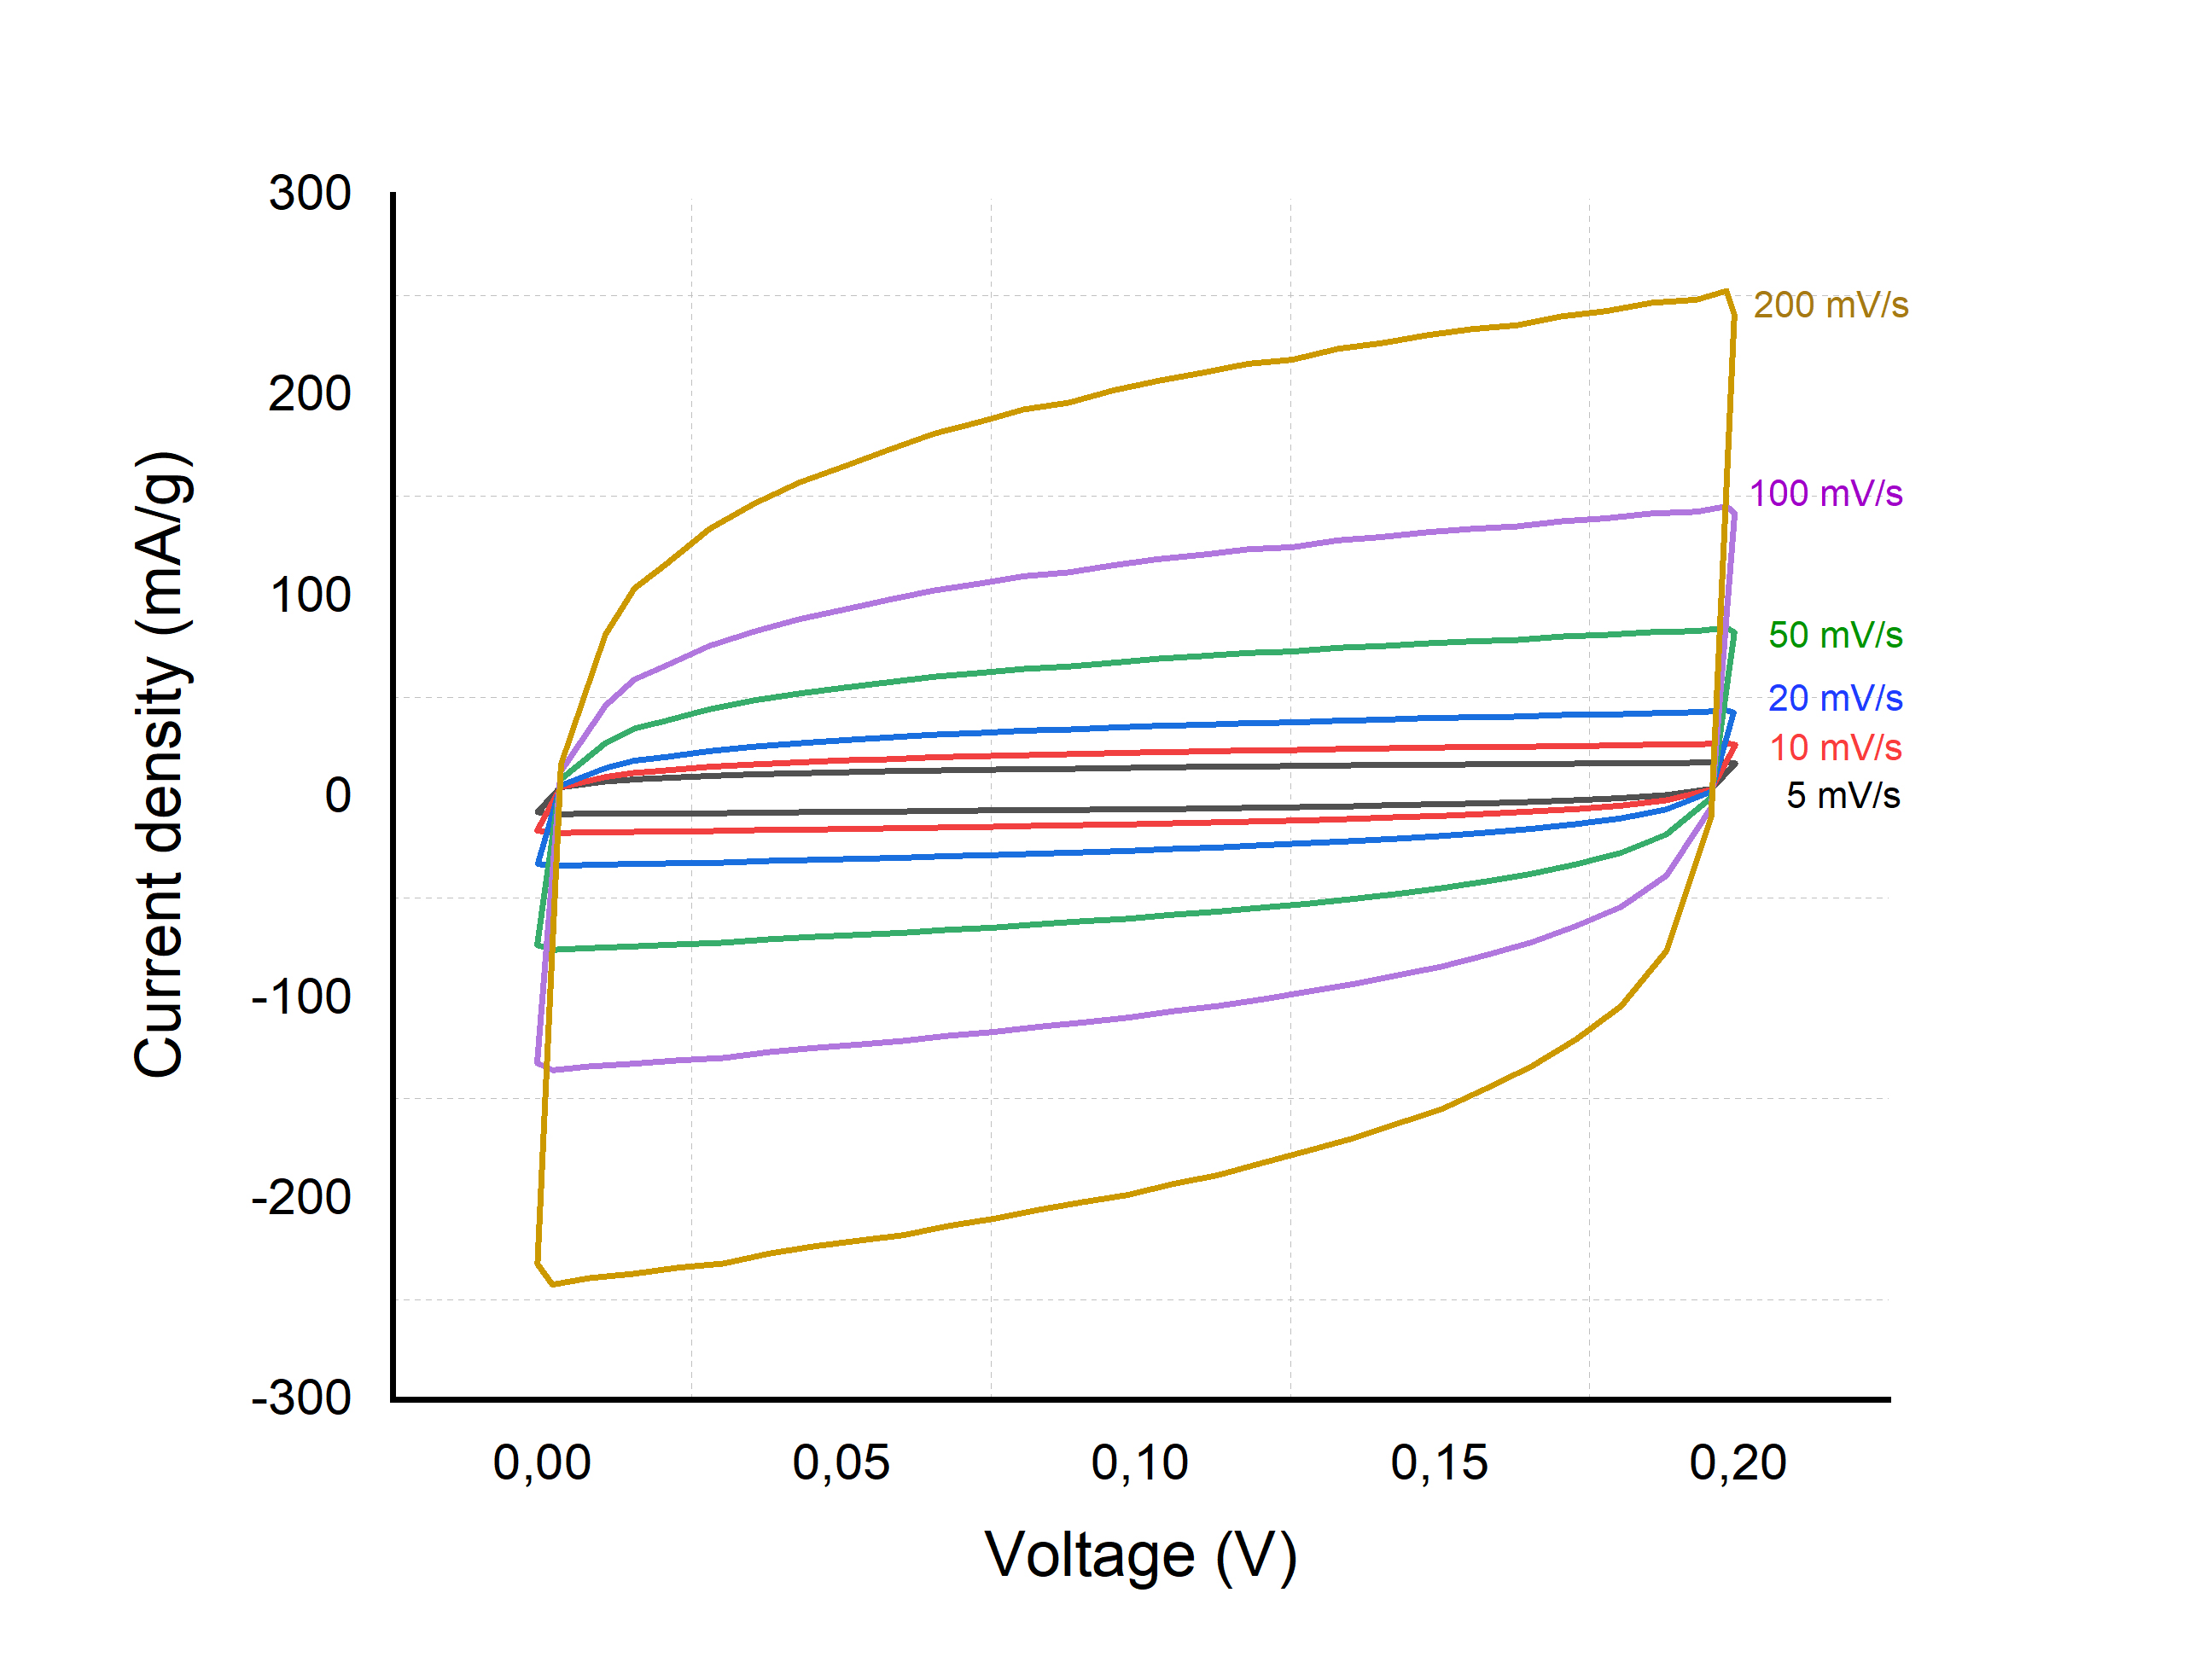
\includegraphics[width=1\textwidth]{Figures/Results/Electrochemistry/LIGP-PI-NaNO3-Swagelok/Cell1/CV_02V_diff_scan_rates-Cell1.jpg} 
\captionsetup{width=0.9\linewidth}
\caption{LIGP-Kapton Electrodes, Cell 1}
\label{fig:LIG-PI-cell1}
\end{subfigure}
\begin{subfigure}{0.49\textwidth}
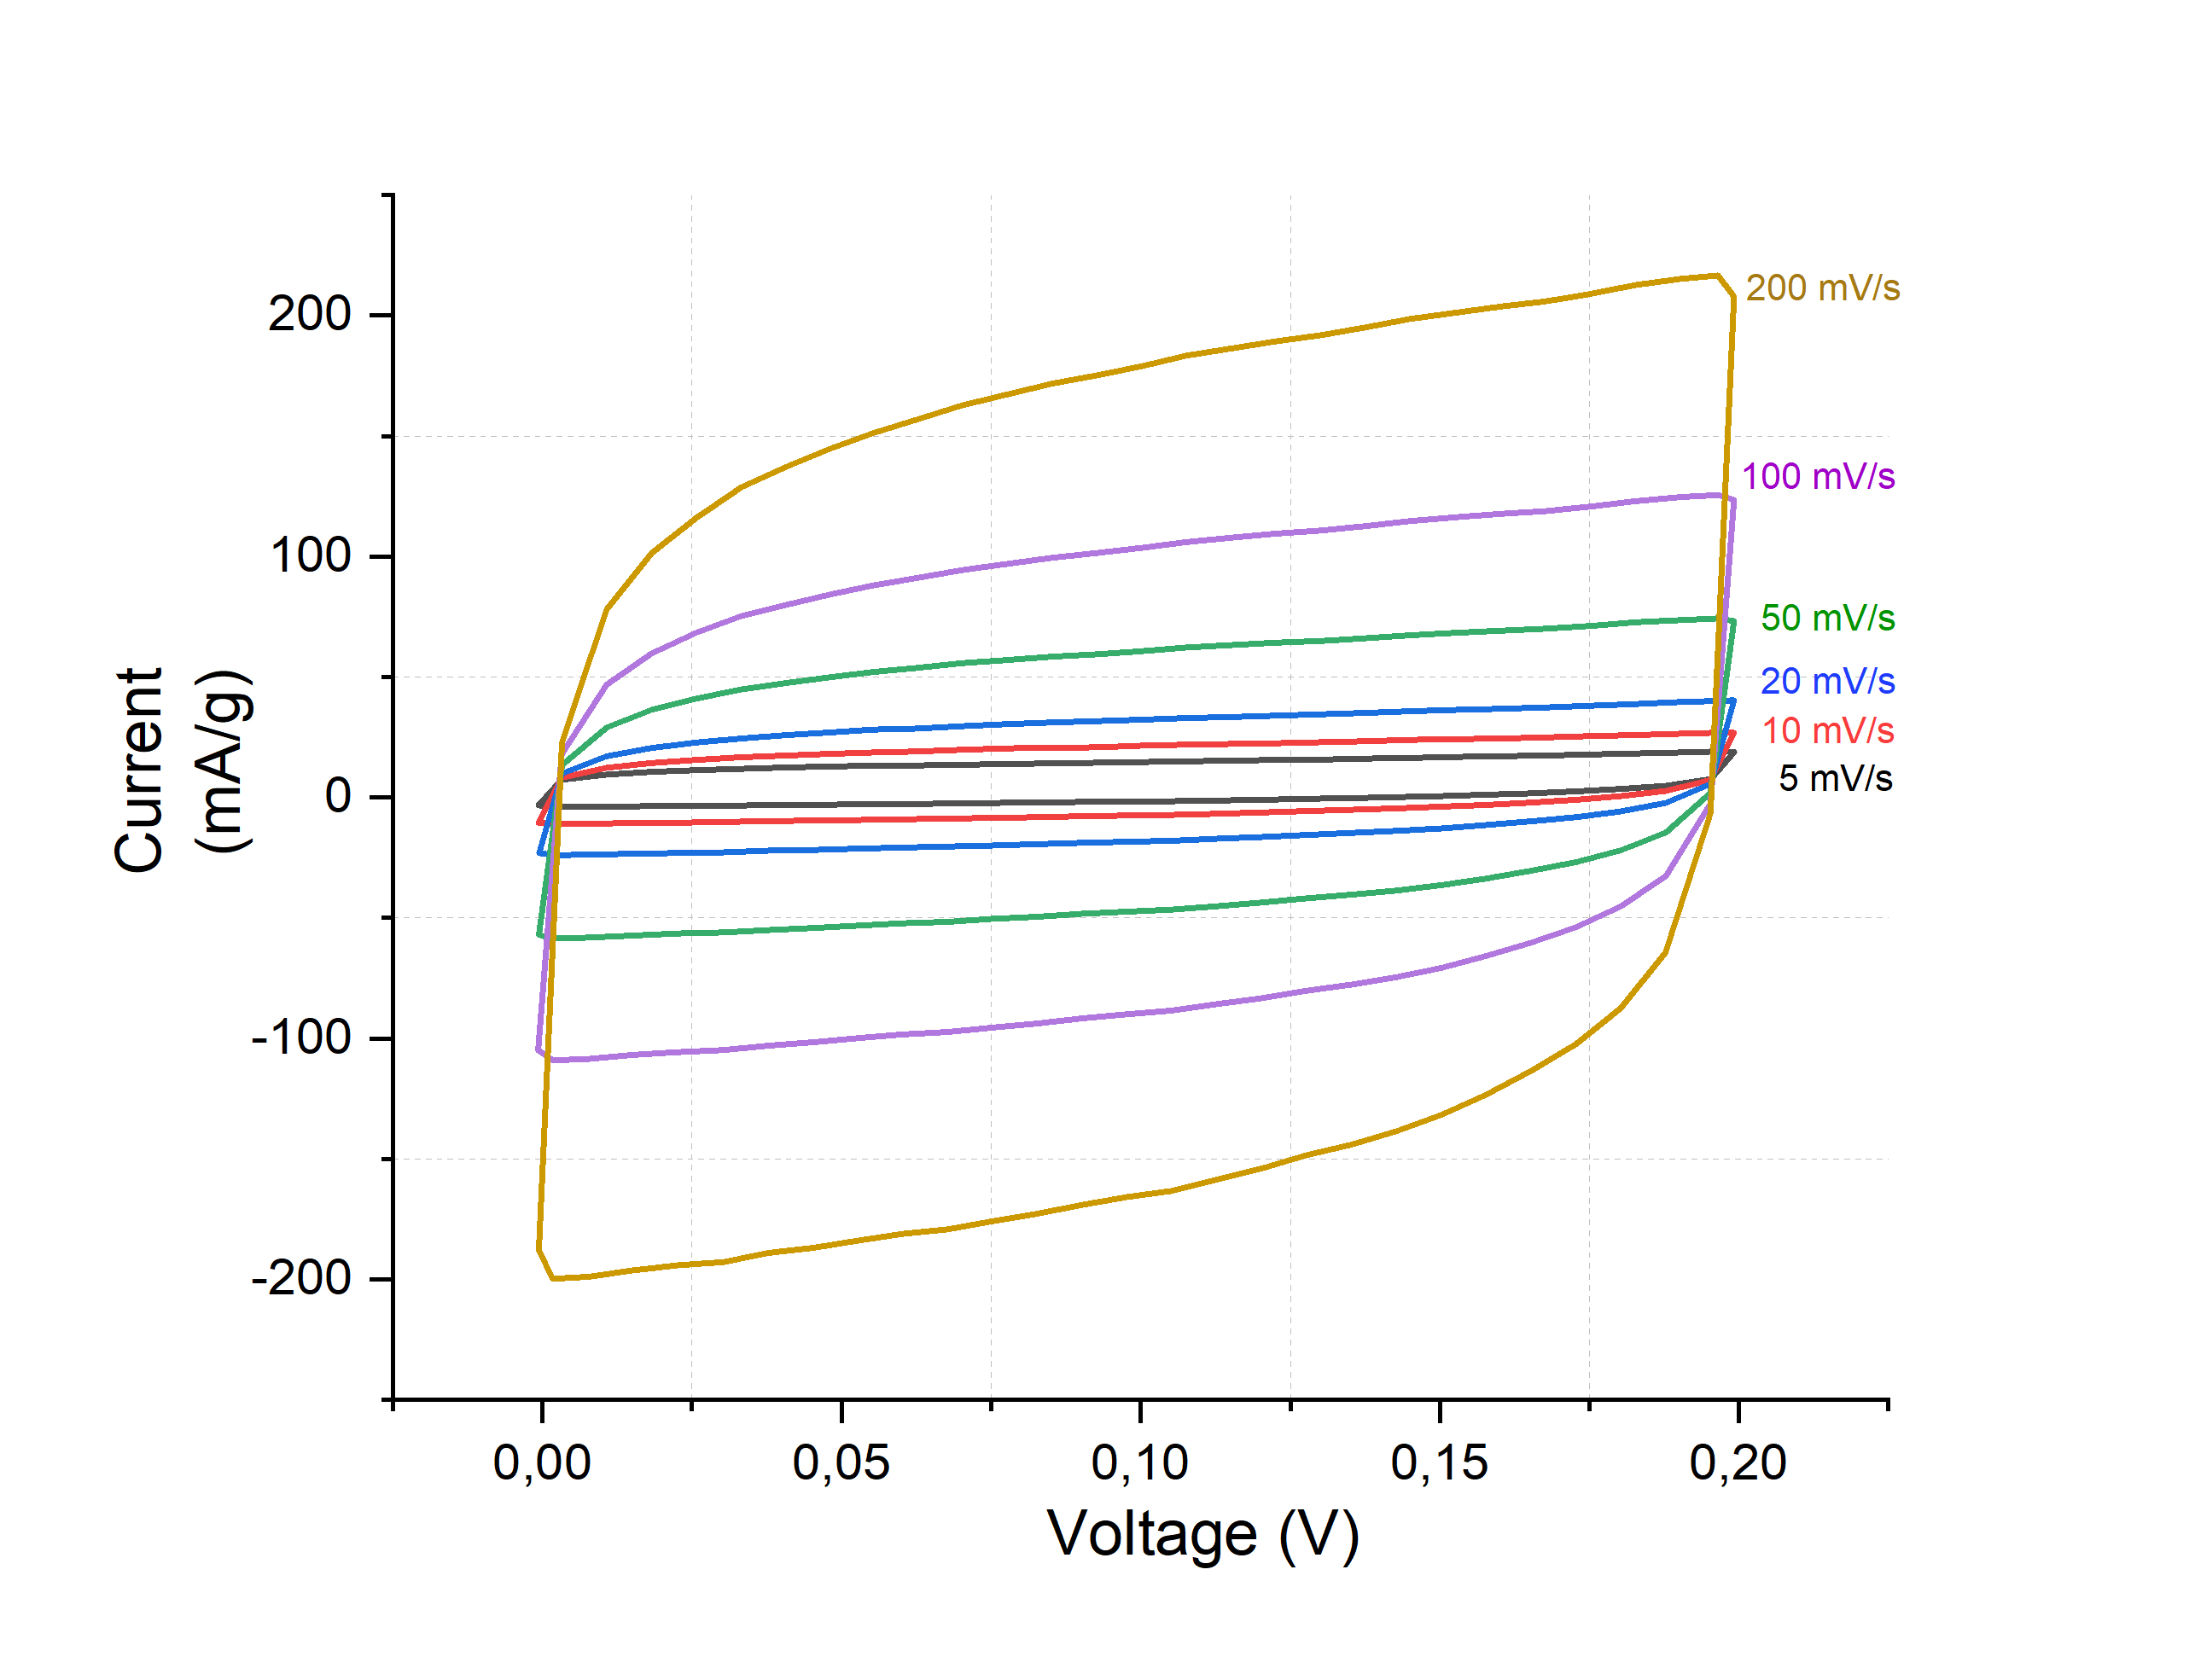
\includegraphics[width=1\textwidth]{Figures/Results/Electrochemistry/LIGP-PI-NaNO3-Swagelok/Cell2/CV_02V_diff_scan_rates-Cell2.jpg}
\captionsetup{width=0.9\linewidth}
\caption{LIGP-Kapton Electrodes, Cell 2}
\label{fig:LIGP-PI-cell2}
\end{subfigure}
\medskip
\caption{CV diagrams of LIGP-Kapton electrodes in Swagelok cells at 0 - 0.2 V potential window at different scan rates}
\label{fig:LIGP-PI-CV-02}
\end{figure}

After the CV sweeping the GCPL measurements were performed for the same voltage window, that is the $V_{max}$ was set to 0.2 V for charging-discharging sets of 10 cycles at the currents of 0.04, 0.1, 0.2, 0.4 and 1 mA for each cycle type. Galvanostatic charge-discharge curves at different current densities as shown in the Figure \ref{fig:LIGP-PI-CC-02} present nearly triangular shapes with minuscule voltage drop indicating negligible internal and contact resistances. For the future comparison with literature data current densities were calculated as $I(V)/m\:[mA/g]$ and $I(V)/s\:[\mu /cm^2]$ and are given for the reference.

\begin{figure}[H]
\begin{subfigure}{0.49\textwidth}
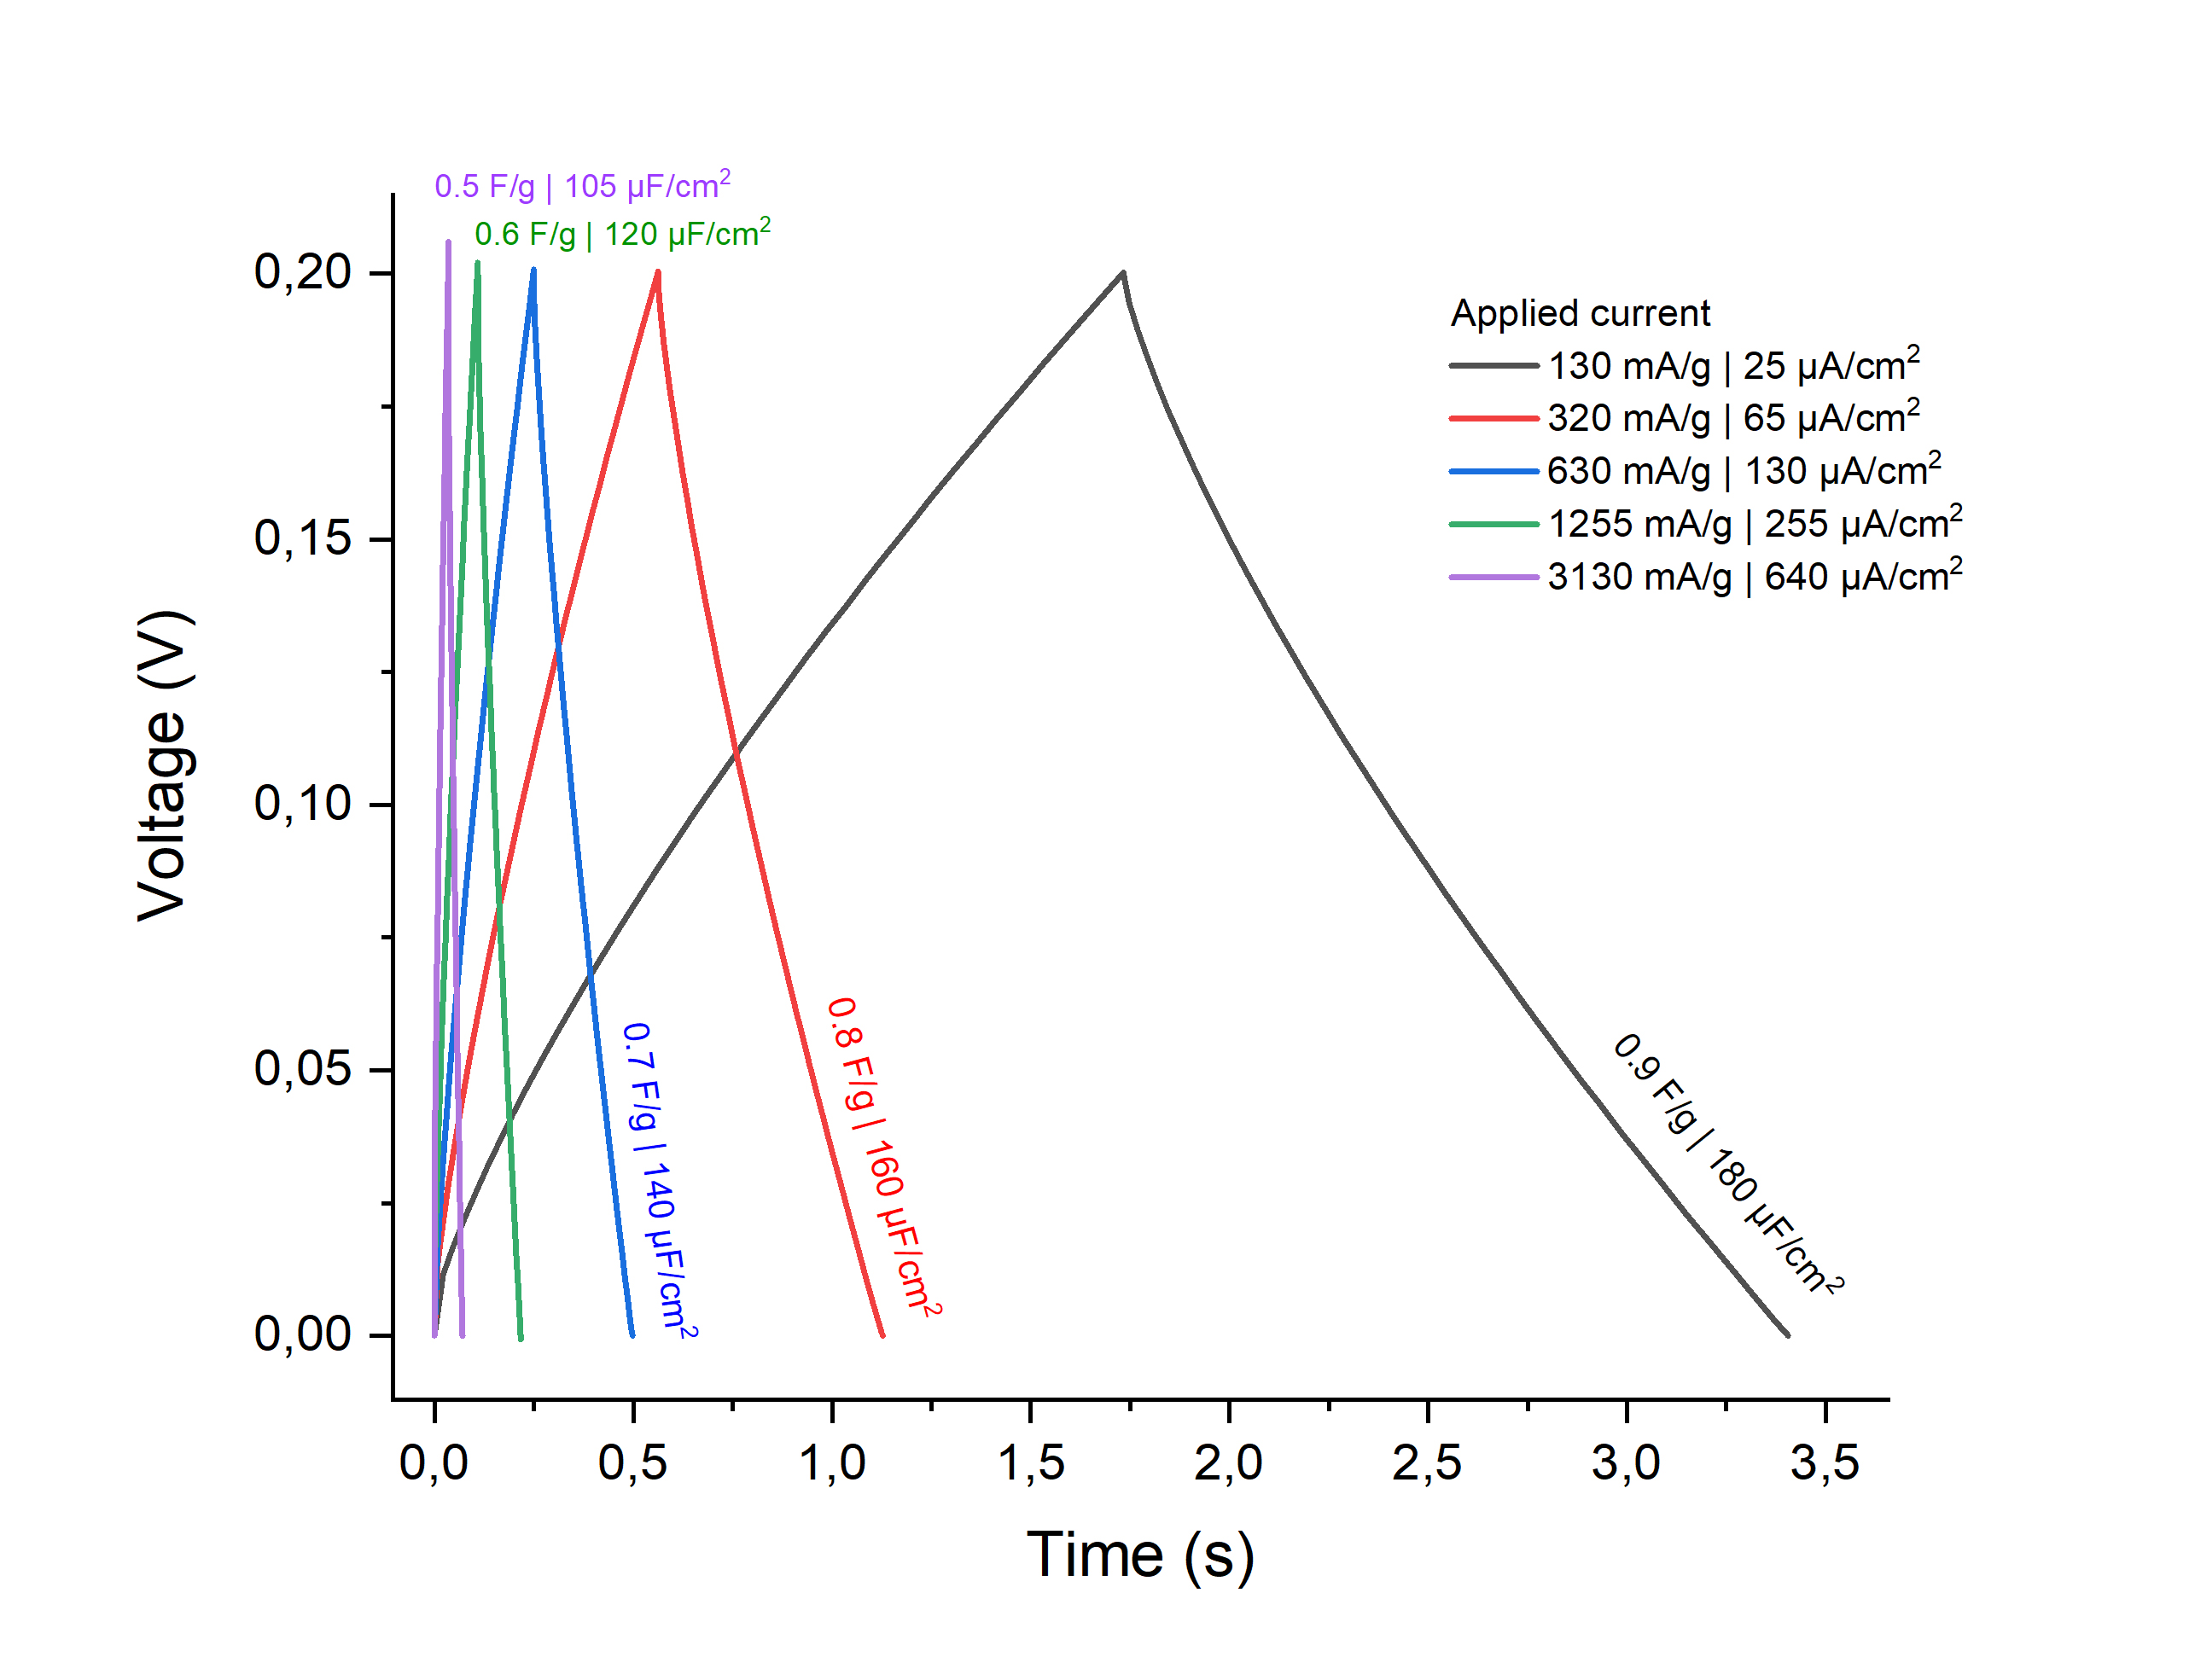
\includegraphics[width=1\textwidth]{Figures/Results/Electrochemistry/LIGP-PI-NaNO3-Swagelok/Cell1/GCPL_Vmax02_cell1_diff-current-Cs.jpg} 
\captionsetup{width=0.9\linewidth}
\caption{LIGP-Kapton Electrodes, Cell 1}
\label{fig:LIG-PI-cell1-CC-02}
\end{subfigure}
\begin{subfigure}{0.49\textwidth}
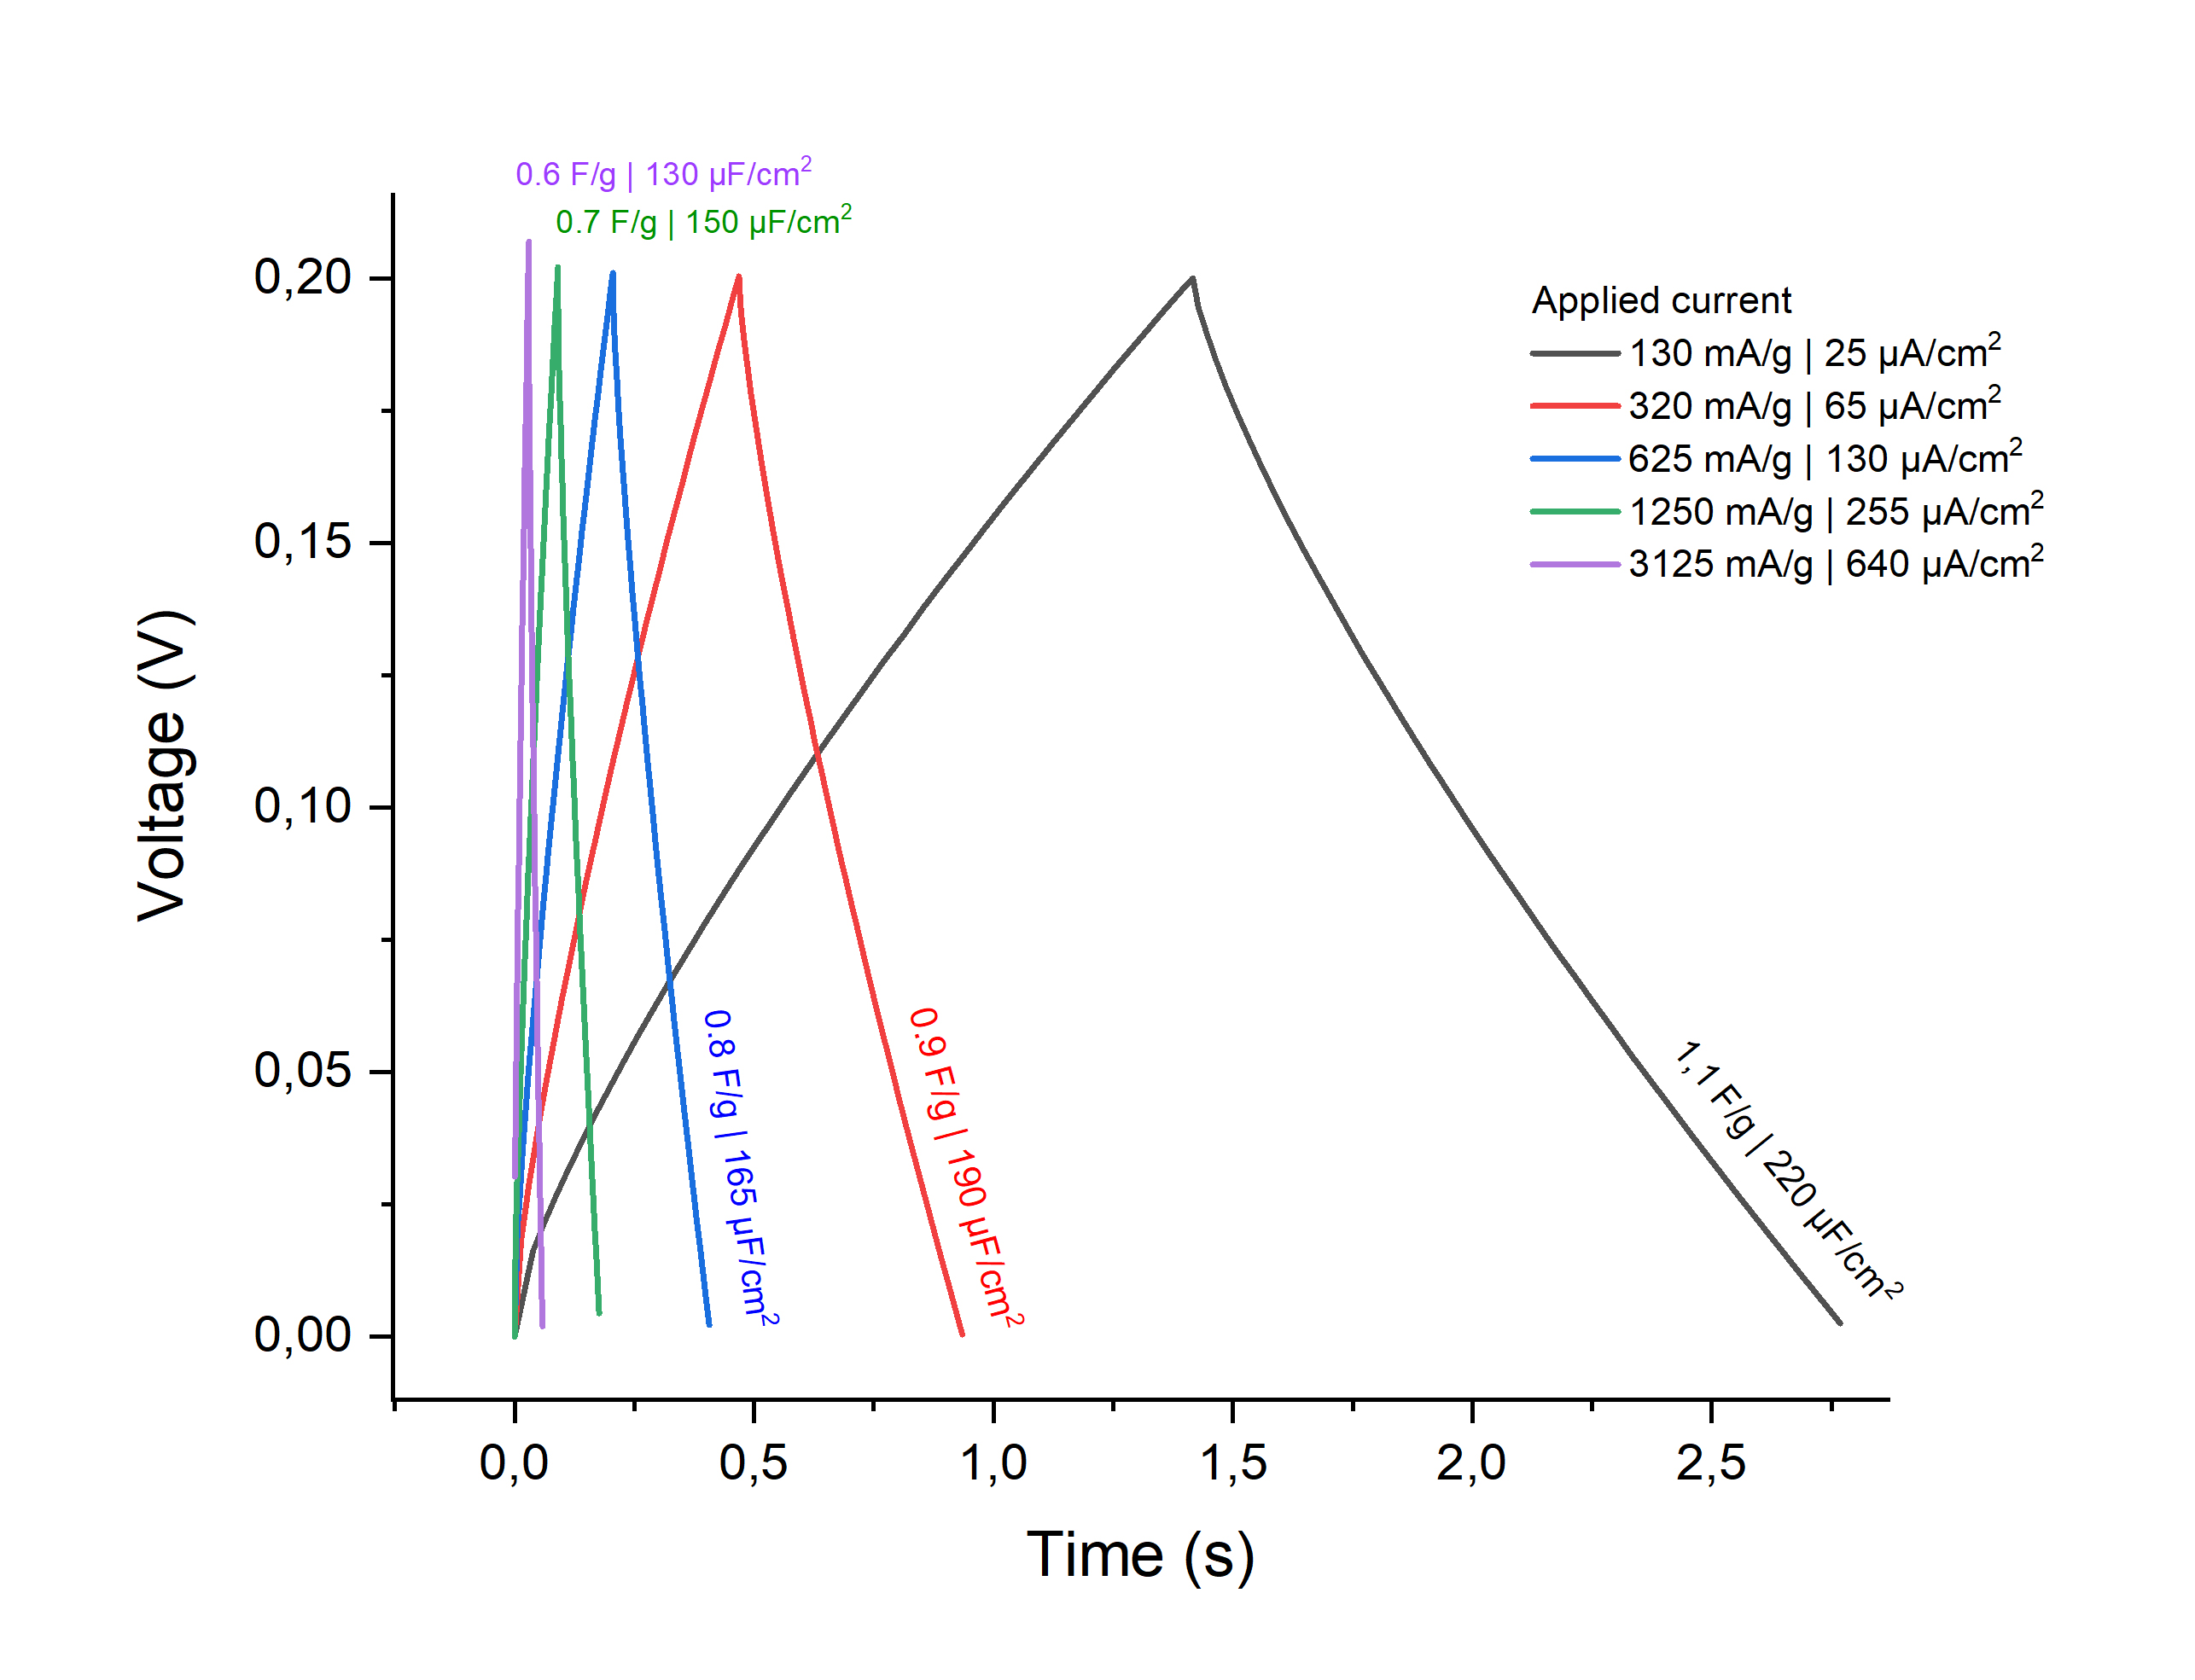
\includegraphics[width=1\textwidth]{Figures/Results/Electrochemistry/LIGP-PI-NaNO3-Swagelok/Cell2/GCPL_Vmax02_cell2_diff-current-Cs.jpg}
\captionsetup{width=0.9\linewidth}
\caption{LIGP-Kapton Electrodes, Cell 2}
\label{fig:LIGP-PI-cell2-CC-02}
\end{subfigure}
\medskip
\caption{CC diagrams of LIGP-Kapton electrodes in Swagelok cells for $V_{max}$=0.2 V at various current densities}
\label{fig:LIGP-PI-CC-02}
\end{figure}

Comparison of the GCPL curves at low vs. high applied currents showed a slightly increasing iR drop as a result of an increasing contact resistance of the electrodes. As can be seen from Figure \ref{fig:LIGP-PI-CC-02-iR-drop} iR changes from 6 mV at 130\:mA/g to 35 mV at 3130\:mA/g. 

\begin{figure}[H]
\begin{subfigure}{0.49\textwidth}
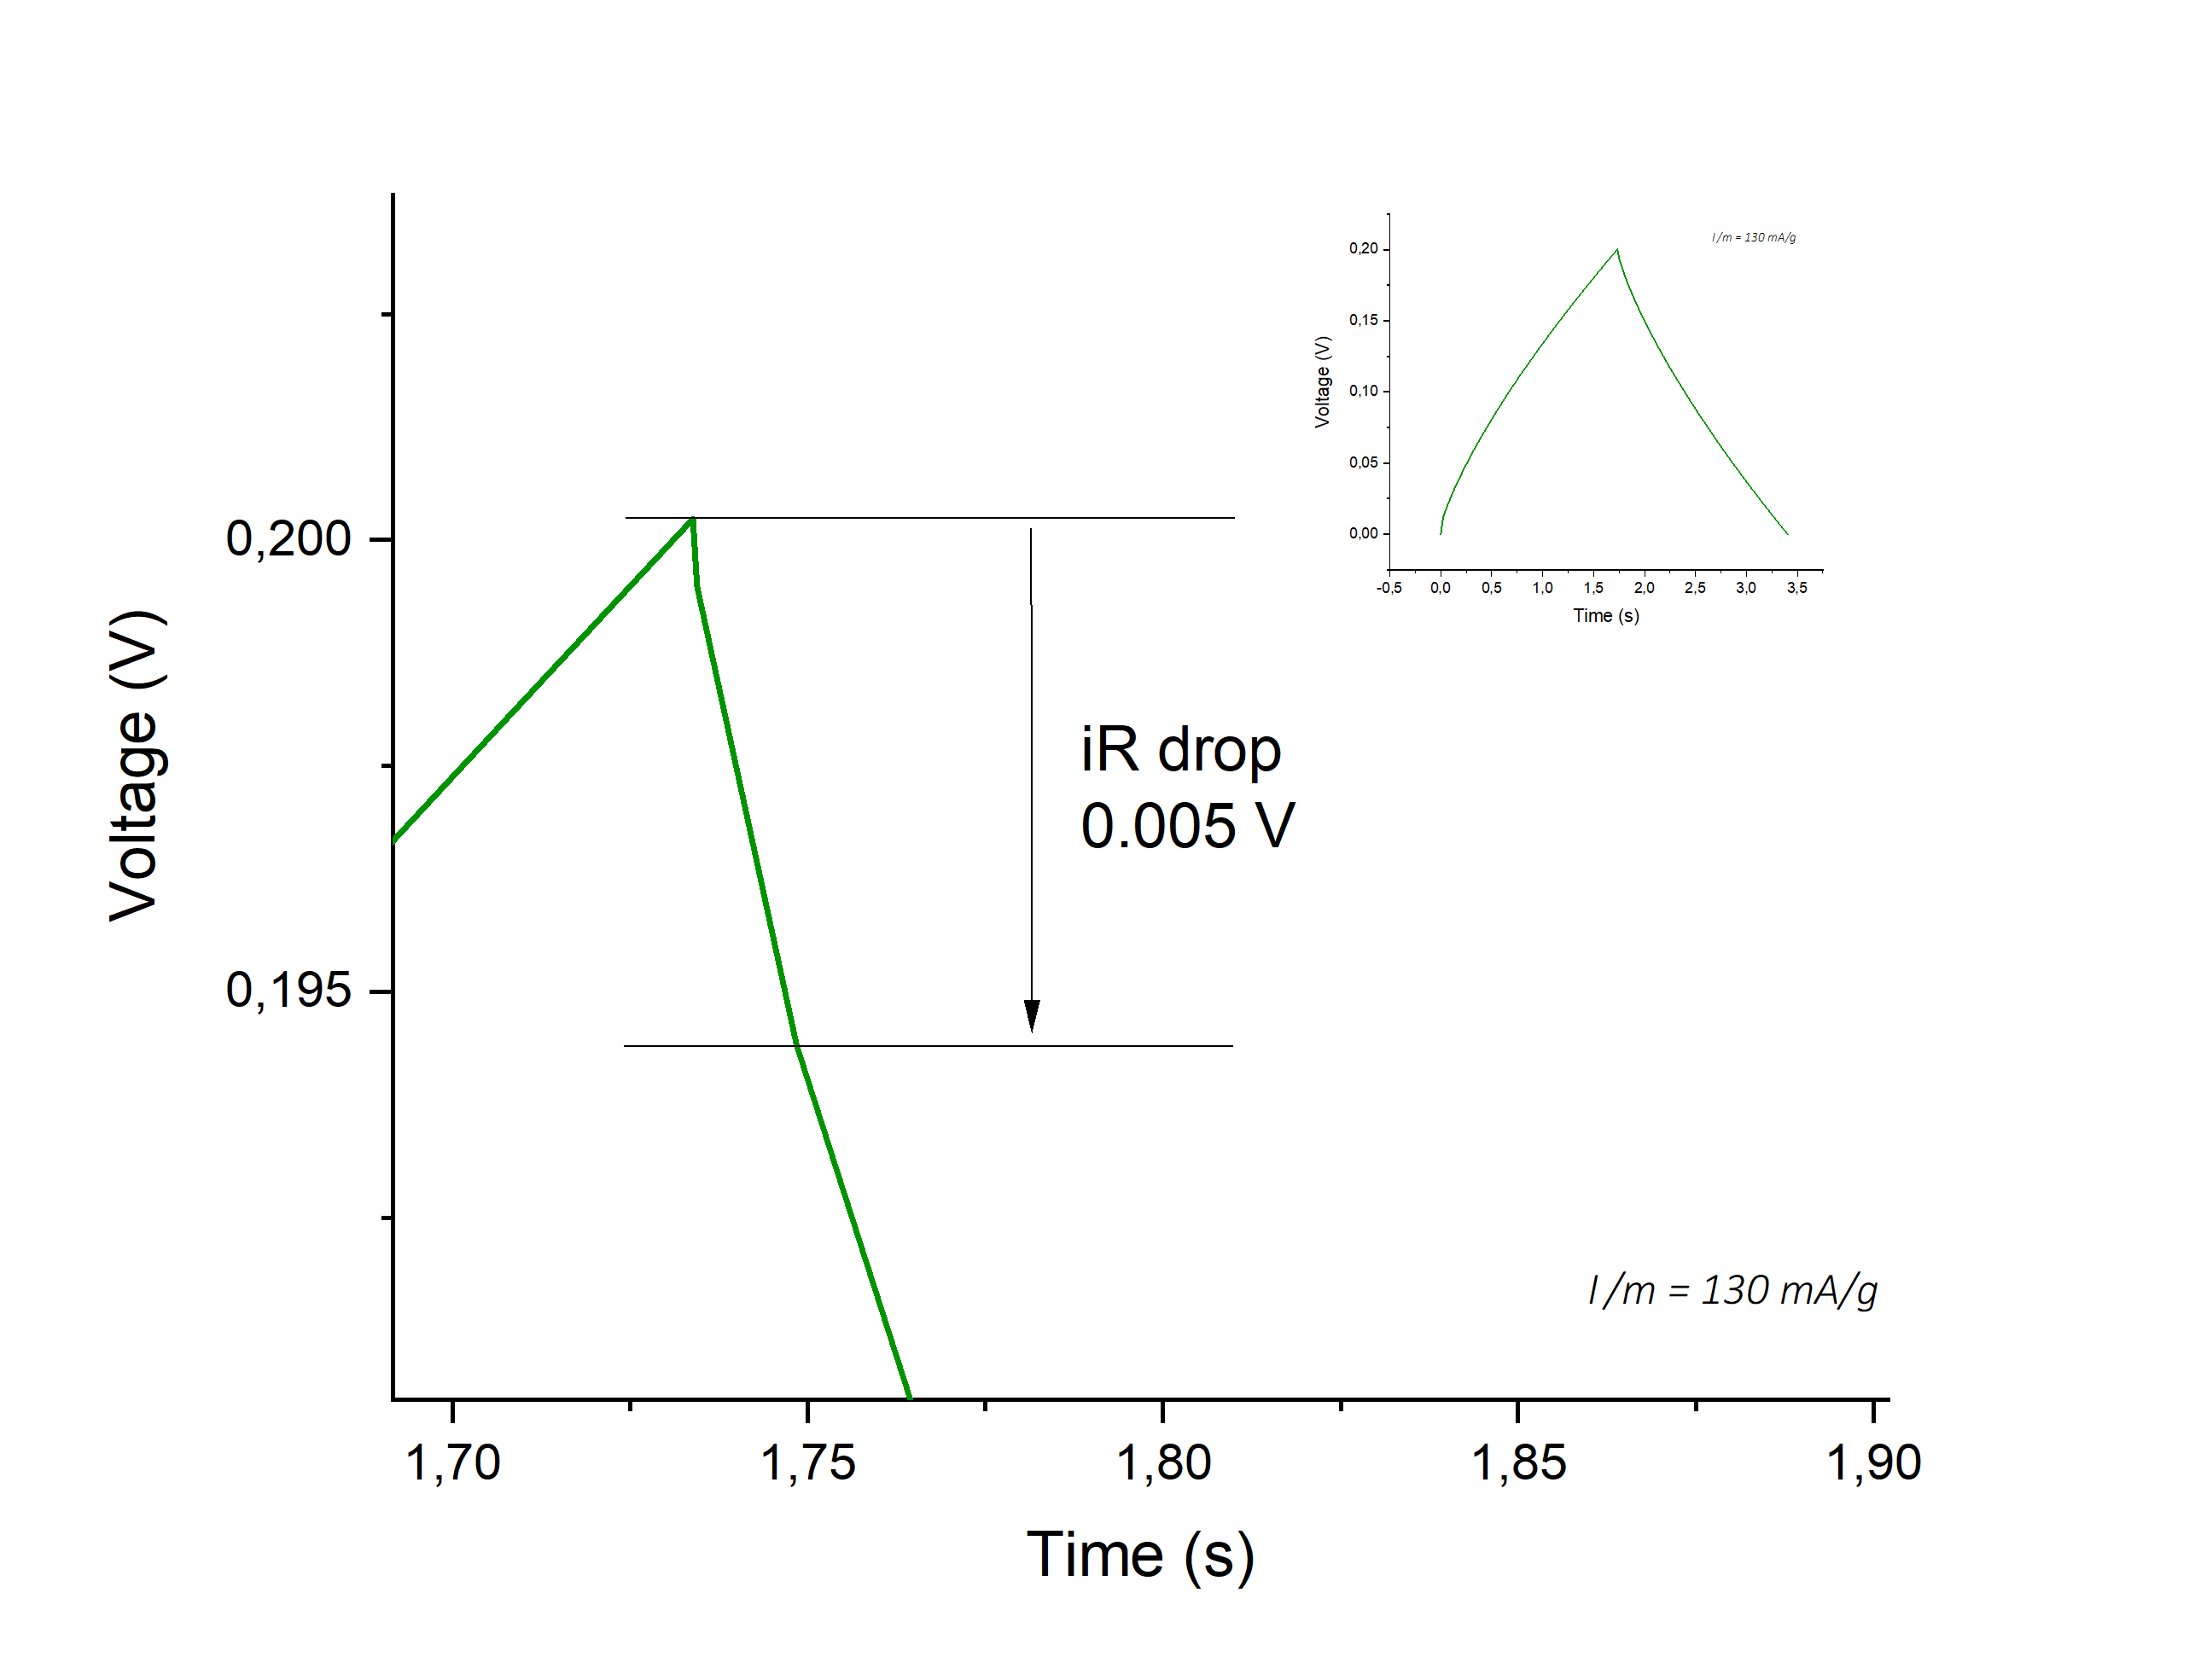
\includegraphics[width=1\textwidth]{Figures/Results/Electrochemistry/LIGP-PI-NaNO3-Swagelok/Cell1/GCPL_Vmax02_cell1_130mA-g-inset.jpg} 
\captionsetup{width=0.9\linewidth}
\caption{LIGP-Kapton Electrodes, Cell 1 at 130\:mA/s}
\label{fig:LIG-PI-cell1-CC-02-iR-low}
\end{subfigure}
\begin{subfigure}{0.49\textwidth}
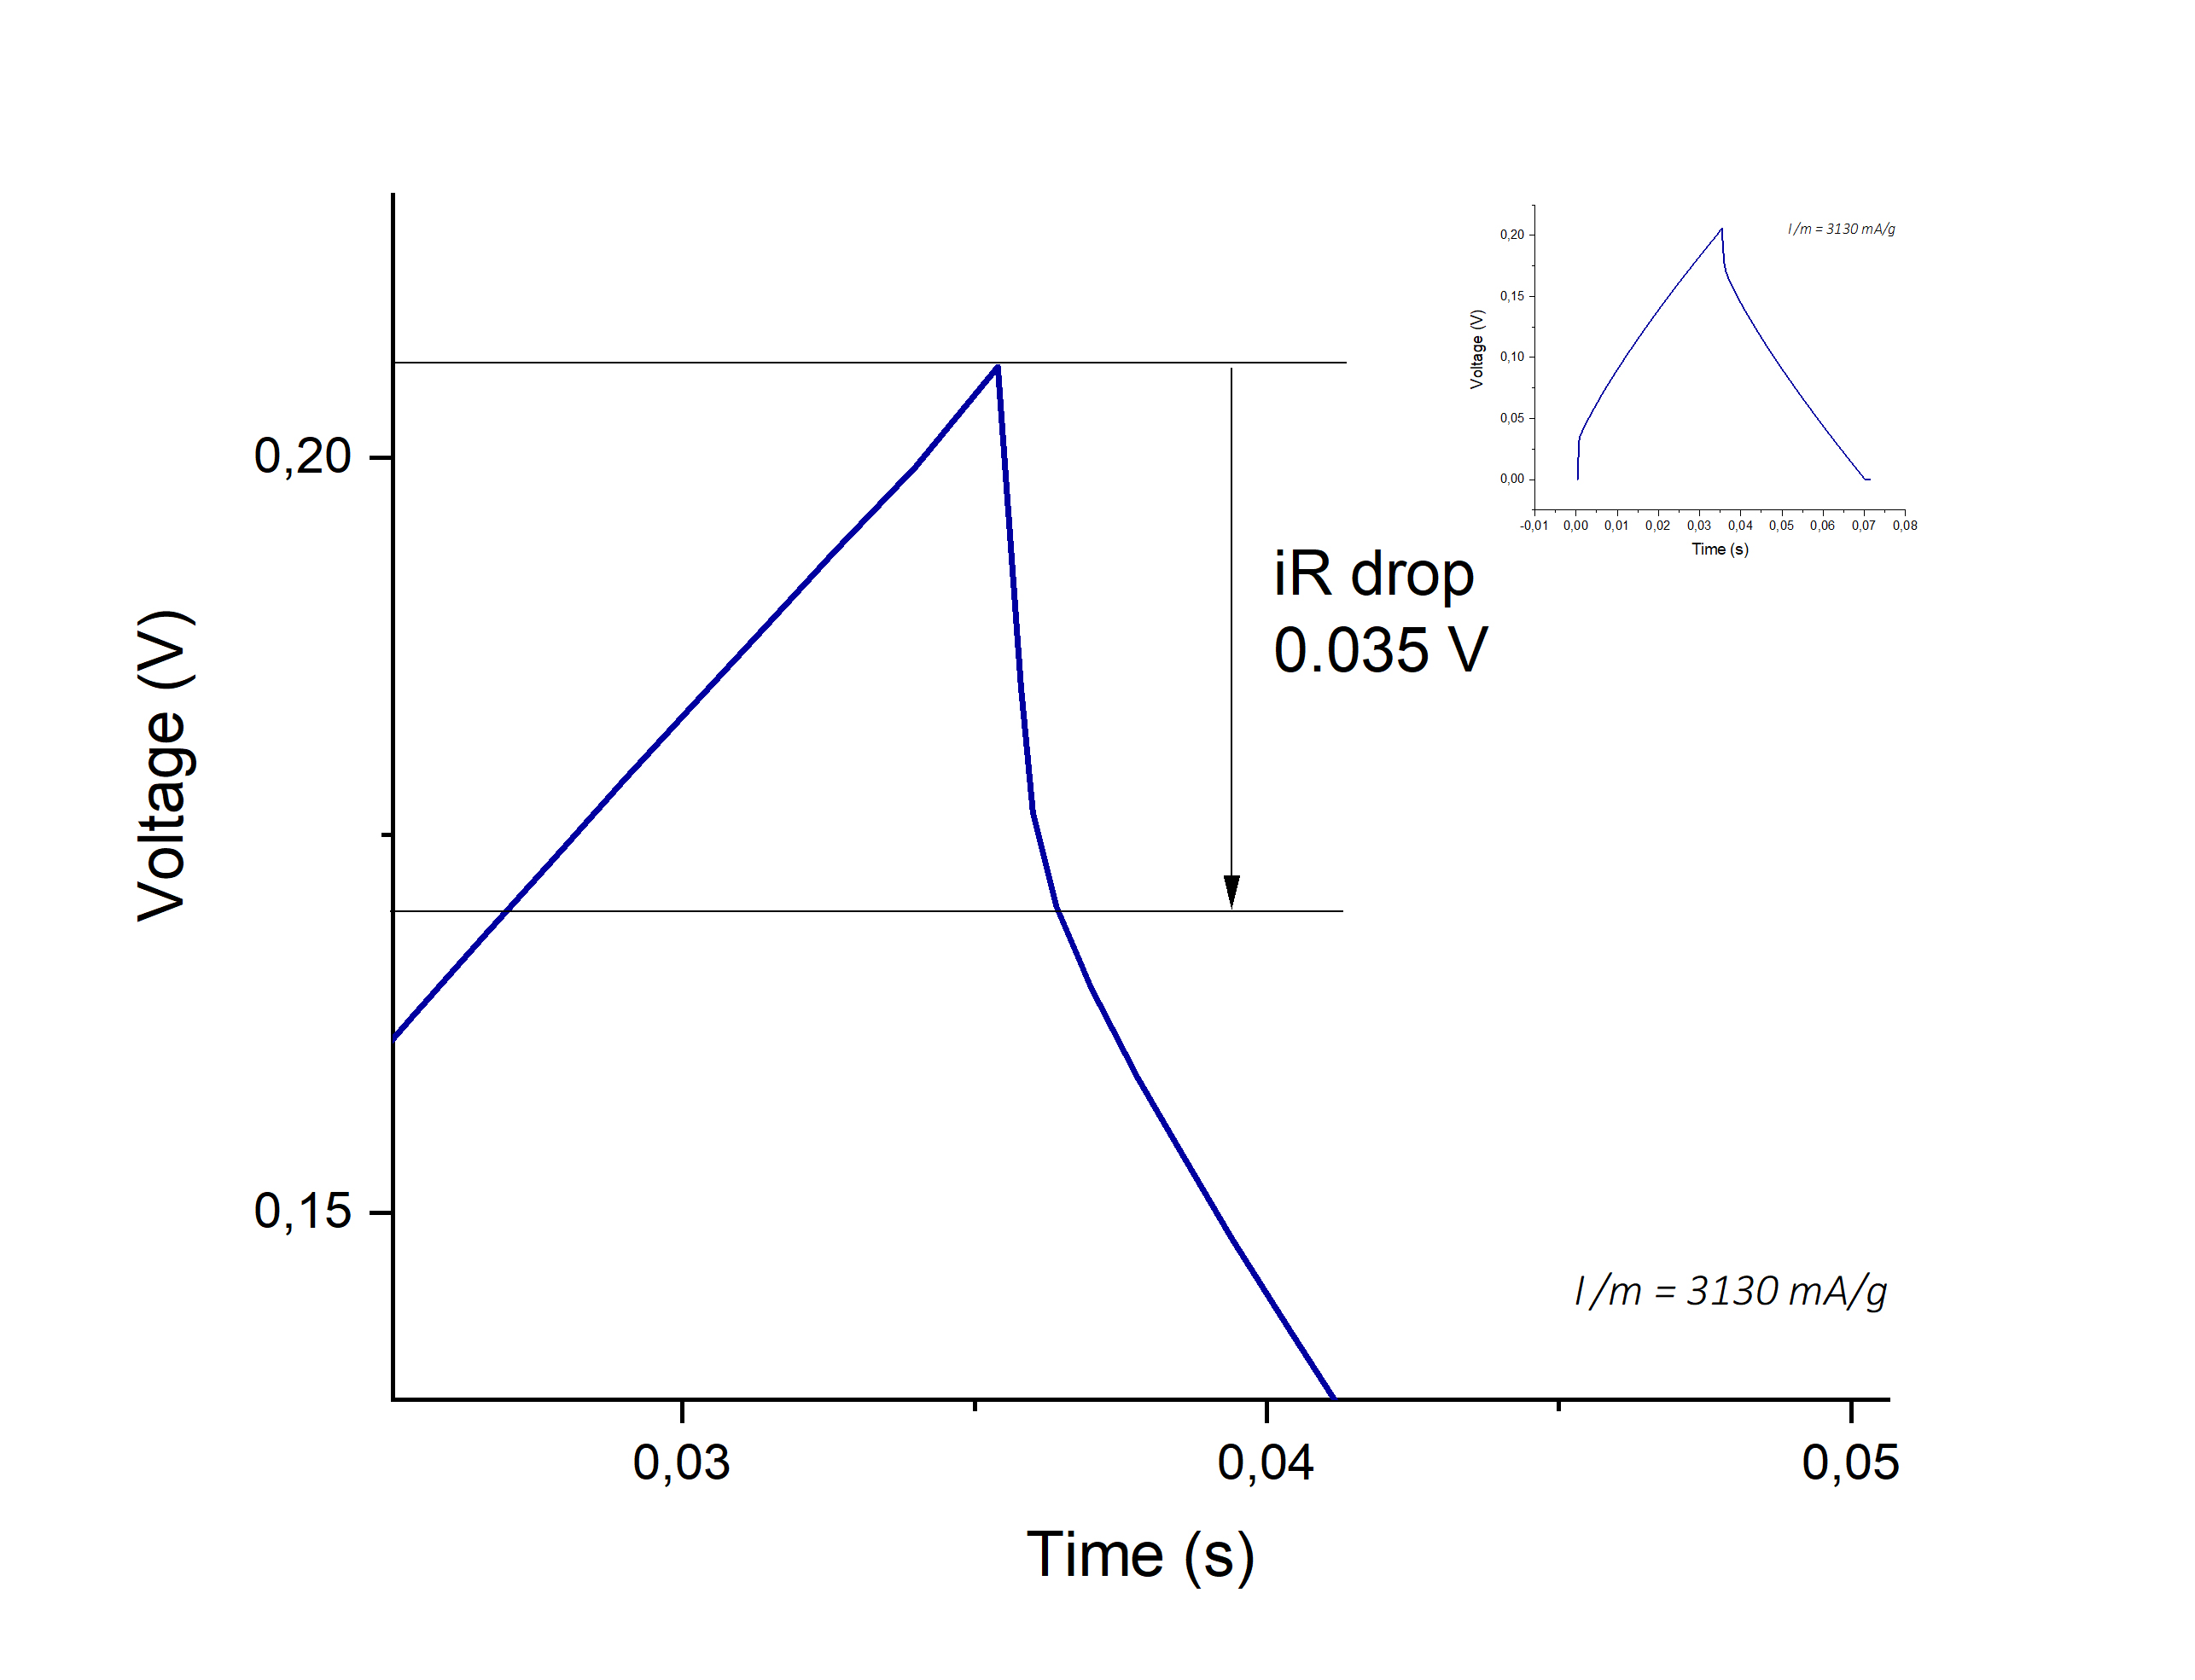
\includegraphics[width=1\textwidth]{Figures/Results/Electrochemistry/LIGP-PI-NaNO3-Swagelok/Cell1/GCPL_Vmax02_cell1_1130mA-g-inset.jpg}
\captionsetup{width=0.9\linewidth}
\caption{LIGP-Kapton Electrodes, Cell 1 at 3130\:mA/s}
\label{fig:LIGP-PI-cell2-CC-02-iR-high}
\end{subfigure}
\medskip
\caption{CC diagrams of LIGP-Kapton electrodes in Swagelok cells for $V_{max}$=0.2 V at 130\:mA/g and 3130\:mA/g demonstrating the rise of iR drop with an increase of applied current}
\label{fig:LIGP-PI-CC-02-iR-drop}
\end{figure}


Further experiments included cyclic voltammetry for larger voltage windows at a constant scan rate of 5mV/s. The cell 1 could be tested for the ranges 0 - 0.6 V, 0 - 0.7 V and 0 - 0.8 V after which the experiment was stopped. The cell 2 was tested for the same potentials as well for the further 0 - 0.9, 0 - 1.0, 0 - 1.1 and 0 - 1.2 V sweeps. For both cells the shape of the CV curve increasingly deteriorated from the originally seen rectangular shape as the voltage window had become wider. The respective cycling diagrams are shown in Figure \ref{fig:LIG-PI-CV-12}. It can be observed that larger potential windows lead for the devices to undergo reversible chemical processes taking place in the cell.

\begin{figure}[H]
\begin{subfigure}{0.49\textwidth}
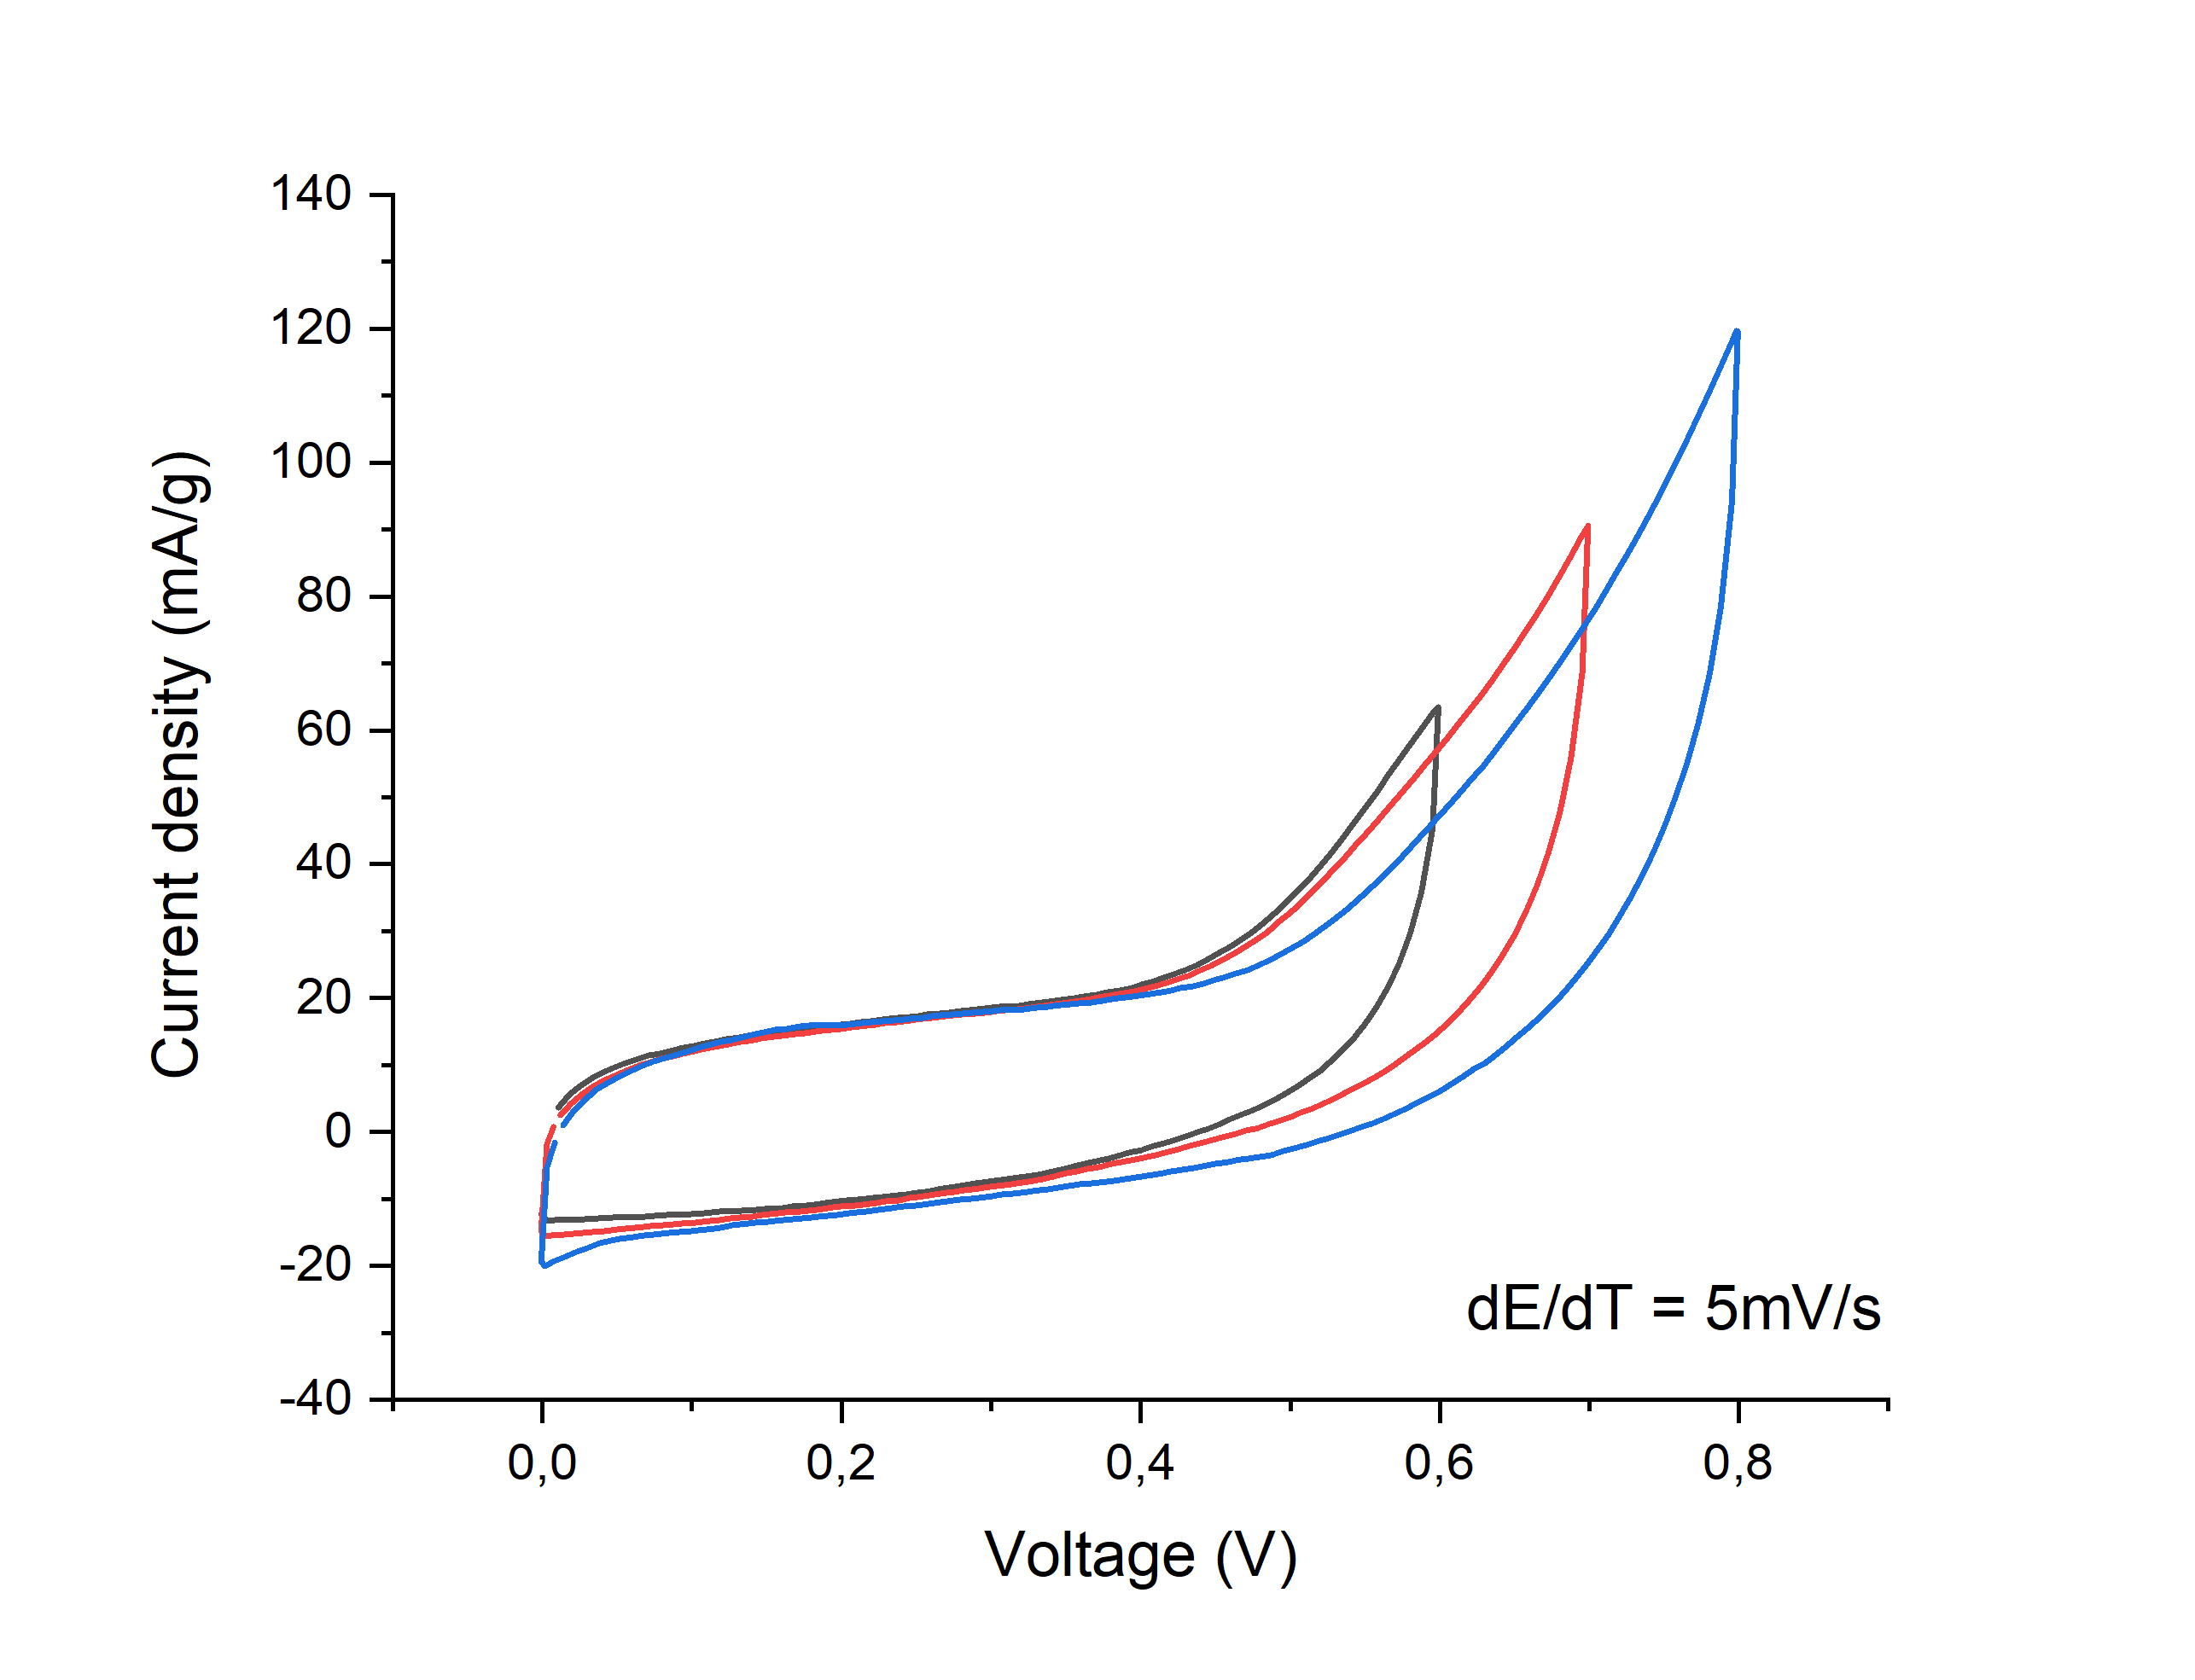
\includegraphics[width=1\textwidth]{Figures/Results/Electrochemistry/LIGP-PI-NaNO3-Swagelok/Cell1/CV-high-V-cell1.jpg} 
\captionsetup{width=0.9\linewidth}
\caption{LIGP-Kapton Electrodes, Cell 1}
\label{fig:LIG-PI-cell1-CV-12}
\end{subfigure}
\begin{subfigure}{0.49\textwidth}
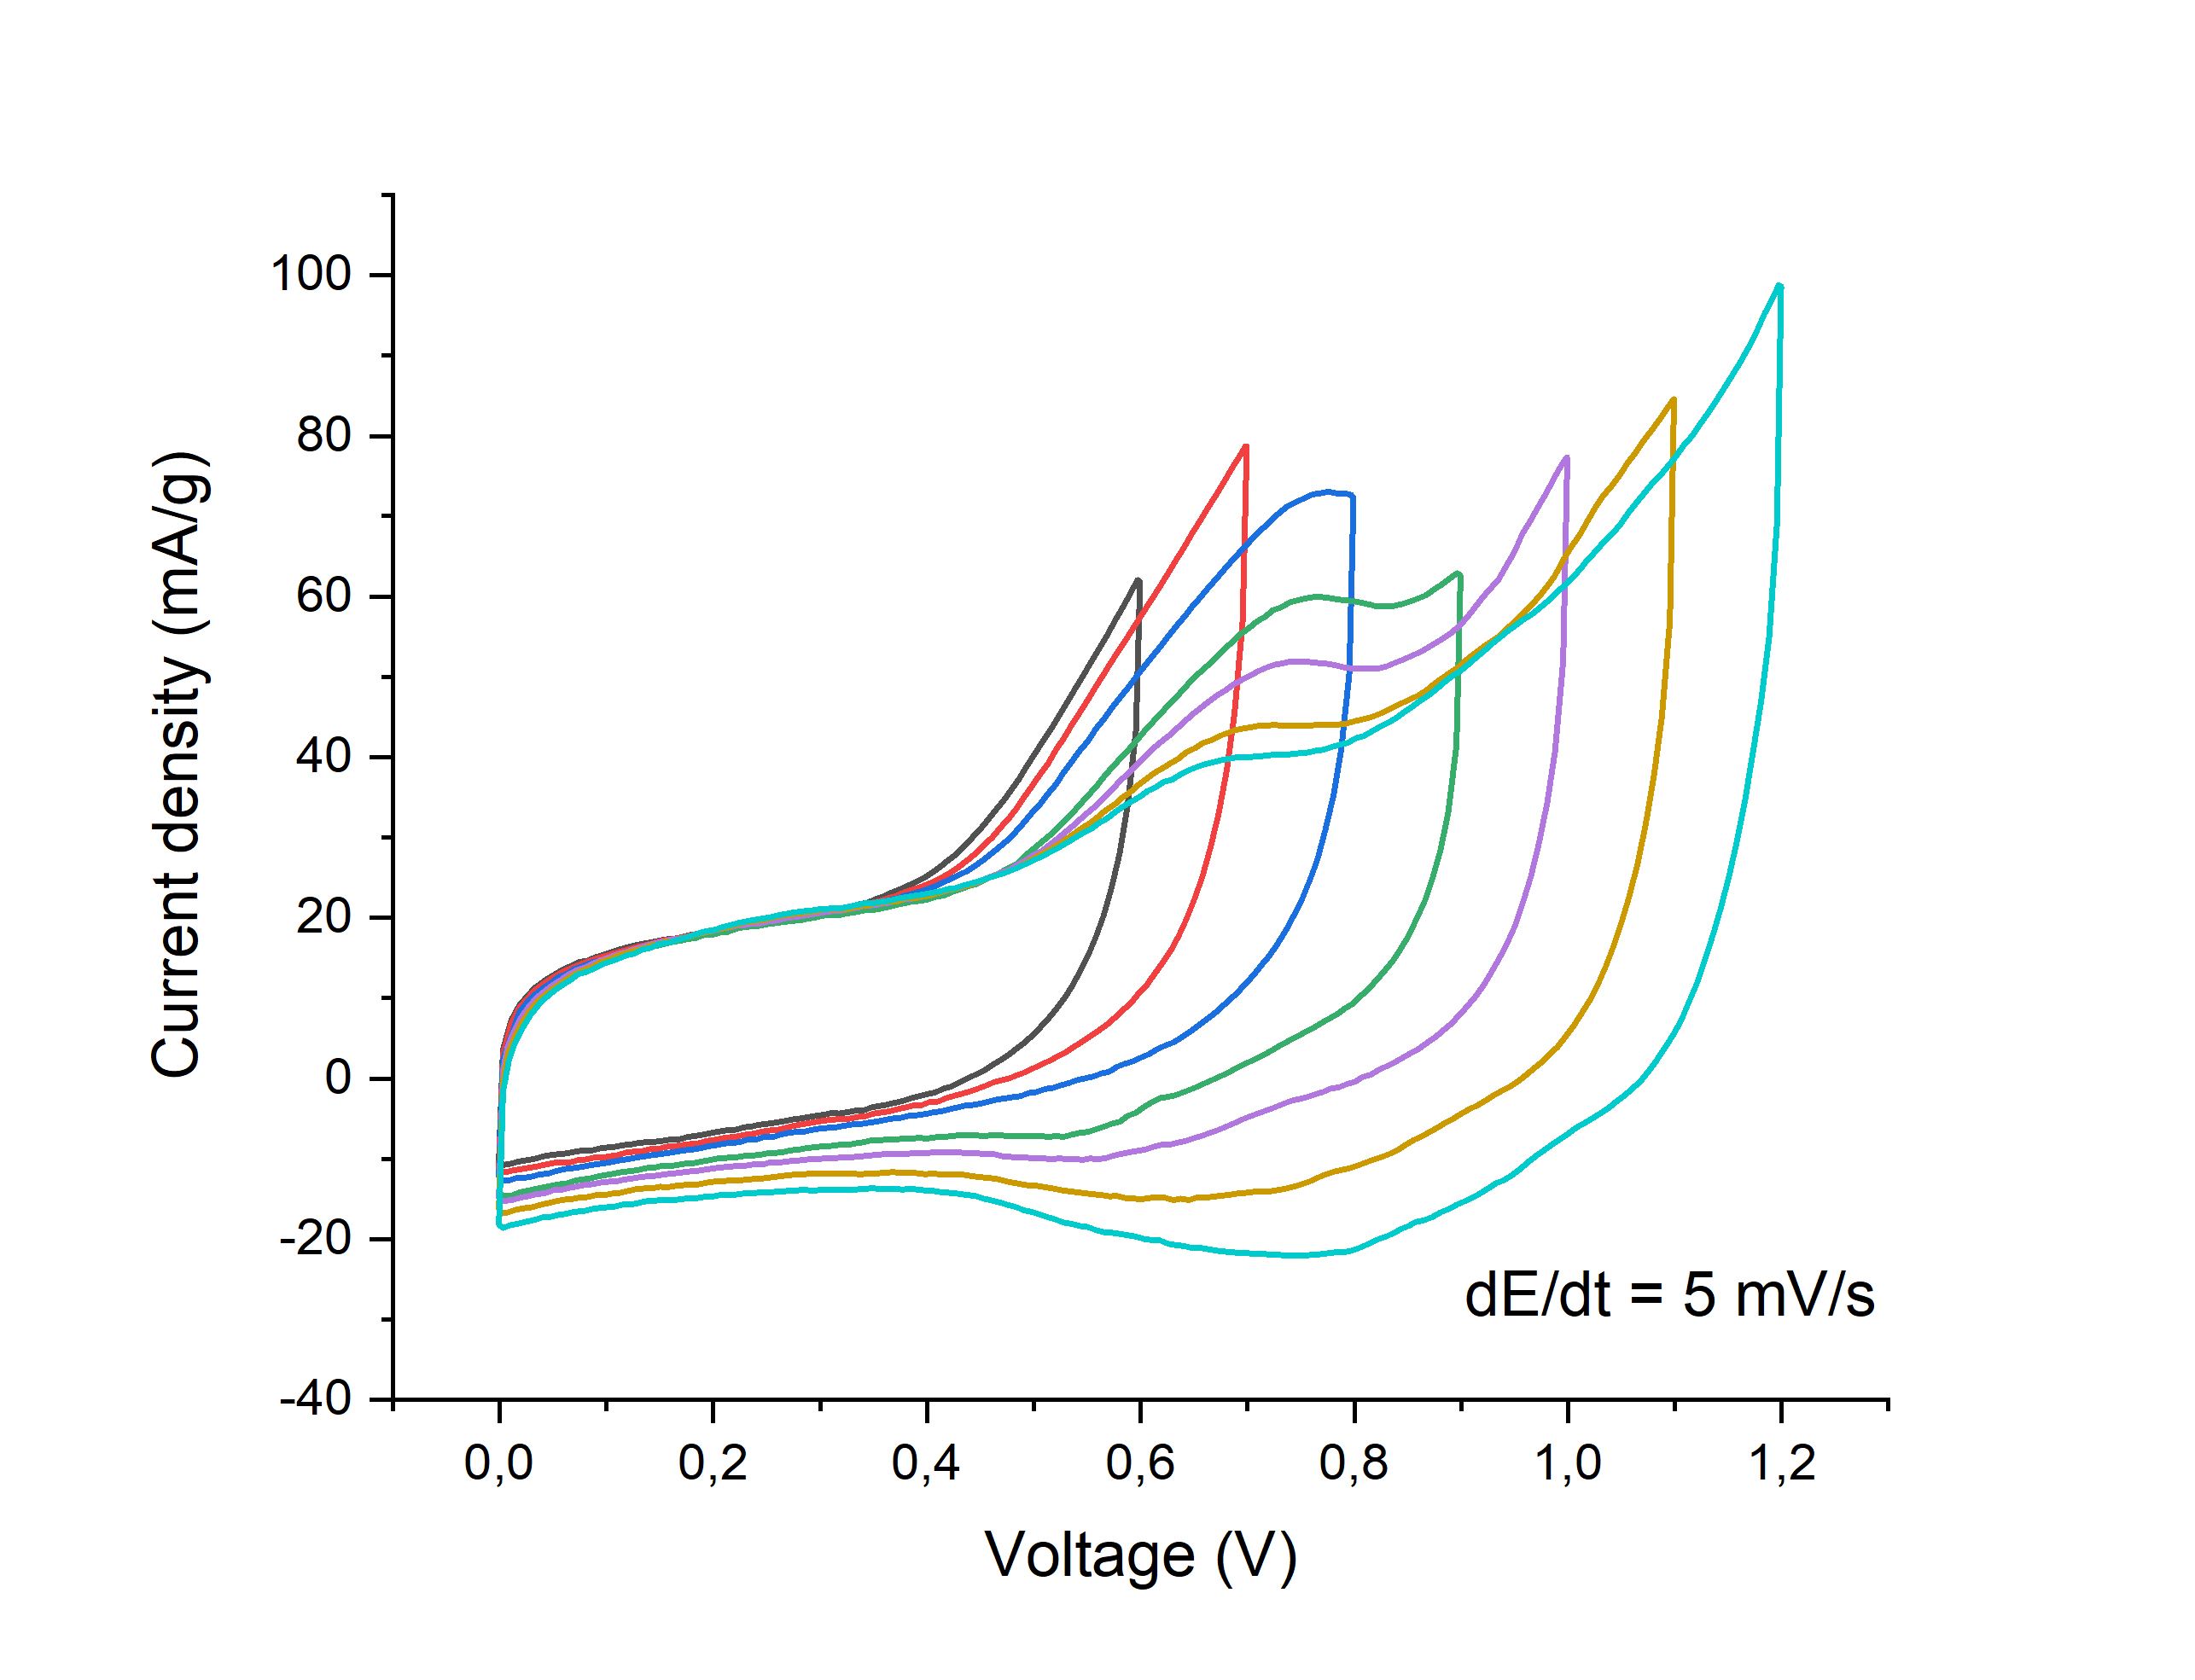
\includegraphics[width=1\textwidth]{Figures/Results/Electrochemistry/LIGP-PI-NaNO3-Swagelok/Cell2/CV-high-volt-cell2.jpg}
\captionsetup{width=0.9\linewidth}
\caption{LIGP-Kapton Electrodes, Cell 2}
\label{fig:LIG-PI-cell2-CV-12}
\end{subfigure}
\medskip
\caption{CV diagrams of LIGP-Kapton electrodes in Swagelok cells for larger $\Delta V$ windows at constant scan rate of 5\:mV/s}
\label{fig:LIG-PI-CV-12}
\end{figure}

Additionally, for the cell 2 the very first CV cycle performed at the $\Delta V$ = 0.6 V showed a characteristic reduction peak on the positive sweep, which did not occur in the following cycles. This peculiarity can be attributed to a non-reversible chemical reaction quickly taking place on an electrode. The cell 1 in turn did not show this peculiarity as can be seen by comparing Figure to Figure : 

\begin{figure}[H]
\begin{subfigure}{0.49\textwidth}
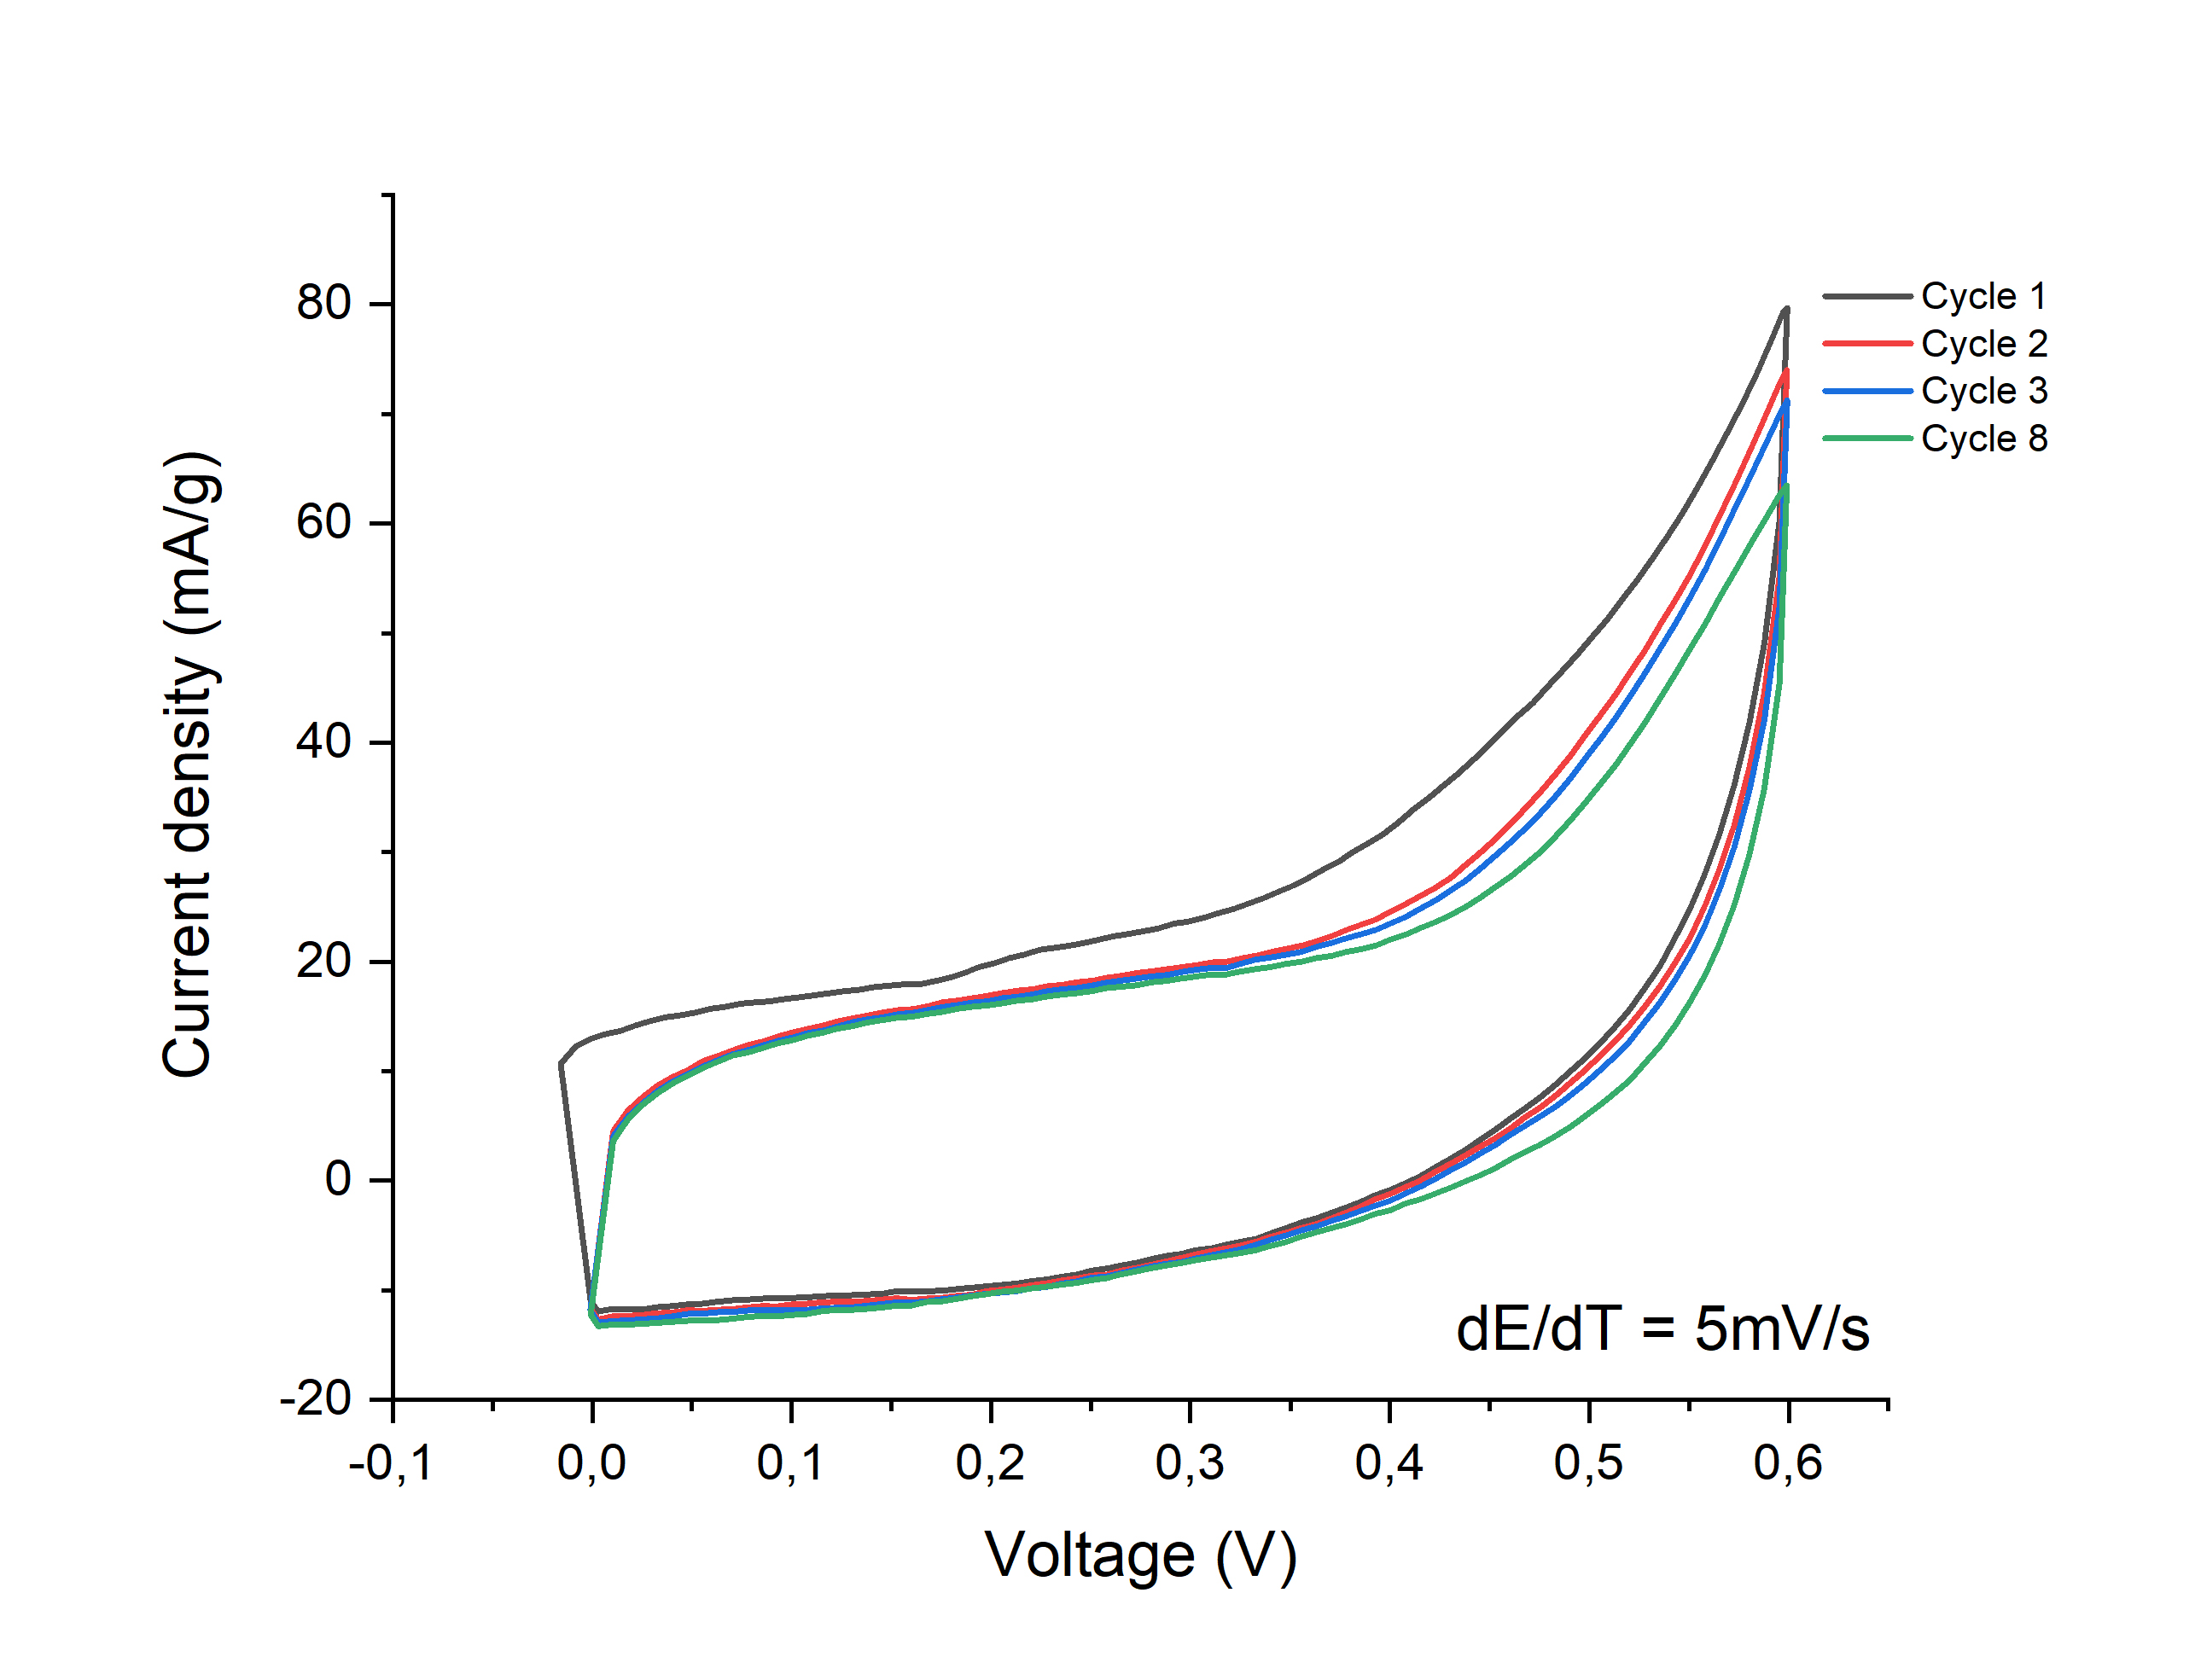
\includegraphics[width=1\textwidth]{Figures/Results/Electrochemistry/LIGP-PI-NaNO3-Swagelok/Cell1/CV-0.6-no-reaction-cell1.jpg} 
\captionsetup{width=0.9\linewidth}
\caption{LIGP-Kapton Electrodes, Cell 1. No peculiar peaks observed}
\label{fig:LIG-PI-cell1-CV-12-noreduction}
\end{subfigure}
\begin{subfigure}{0.49\textwidth}
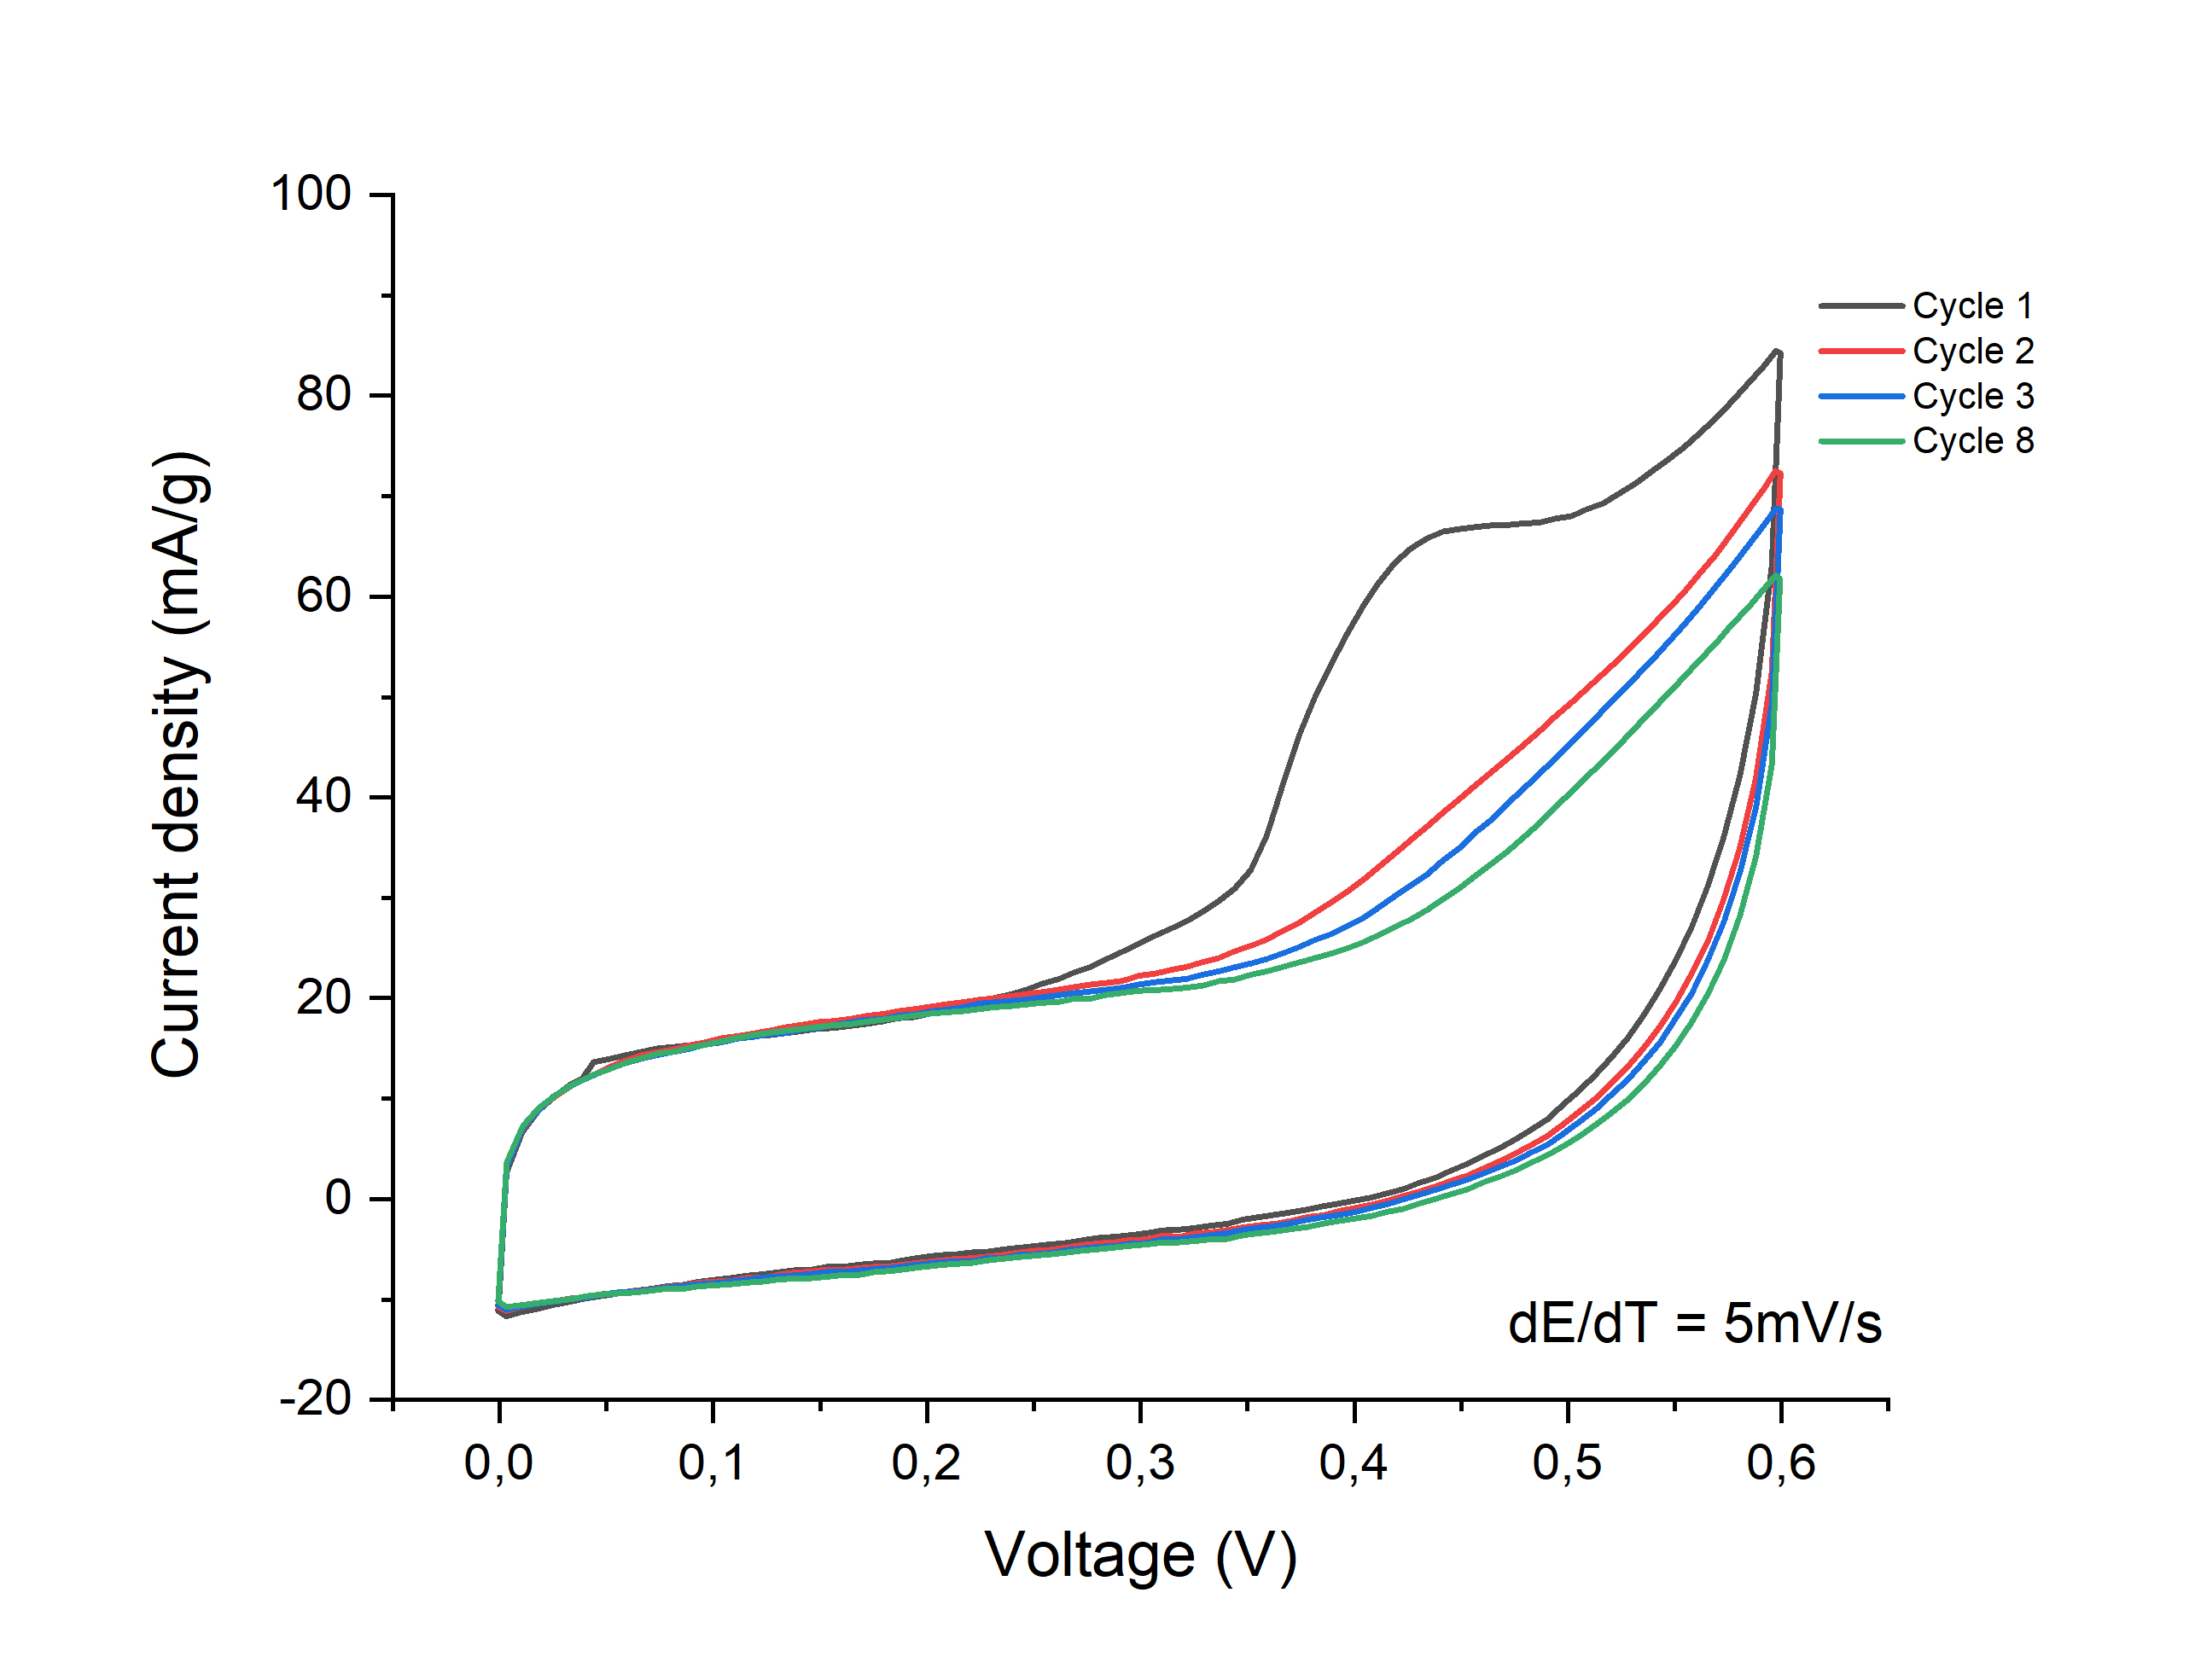
\includegraphics[width=1\textwidth]{Figures/Results/Electrochemistry/LIGP-PI-NaNO3-Swagelok/Cell2/Reaction-higher-volt-Cell2.jpg}
\captionsetup{width=0.9\linewidth}
\caption{LIGP-Kapton Electrodes, Cell 2. Characteristic Peak on the positive sweep at first cycle}
\label{fig:LIG-PI-cell2-CV-12-reduction}
\end{subfigure}
\medskip
\caption{CV diagrams of LIGP-Kapton electrodes in Swagelok cells for $\Delta V$ = 0.6\:V at a constant scan rate of 5\:mV/s}
\label{fig:LIG-PI-CV-06}
\end{figure}

After each series of voltammetry cycles a set of galvanostatic cycles at repeatedly the same applied current of 320\:mA/g was put into run. At higher voltages the triangular shape of the CC curves stayed satisfyingly similar to the lower voltages, showing the same slope of the discharge branches. This fact is consistent with Equation \ref{eq:Capacitance-GC} and serves as an indication that the capacitance performance of the devices stayed constant independently of the $V_{max}$ rise.  

\begin{figure}[H]
\begin{subfigure}{0.49\textwidth}
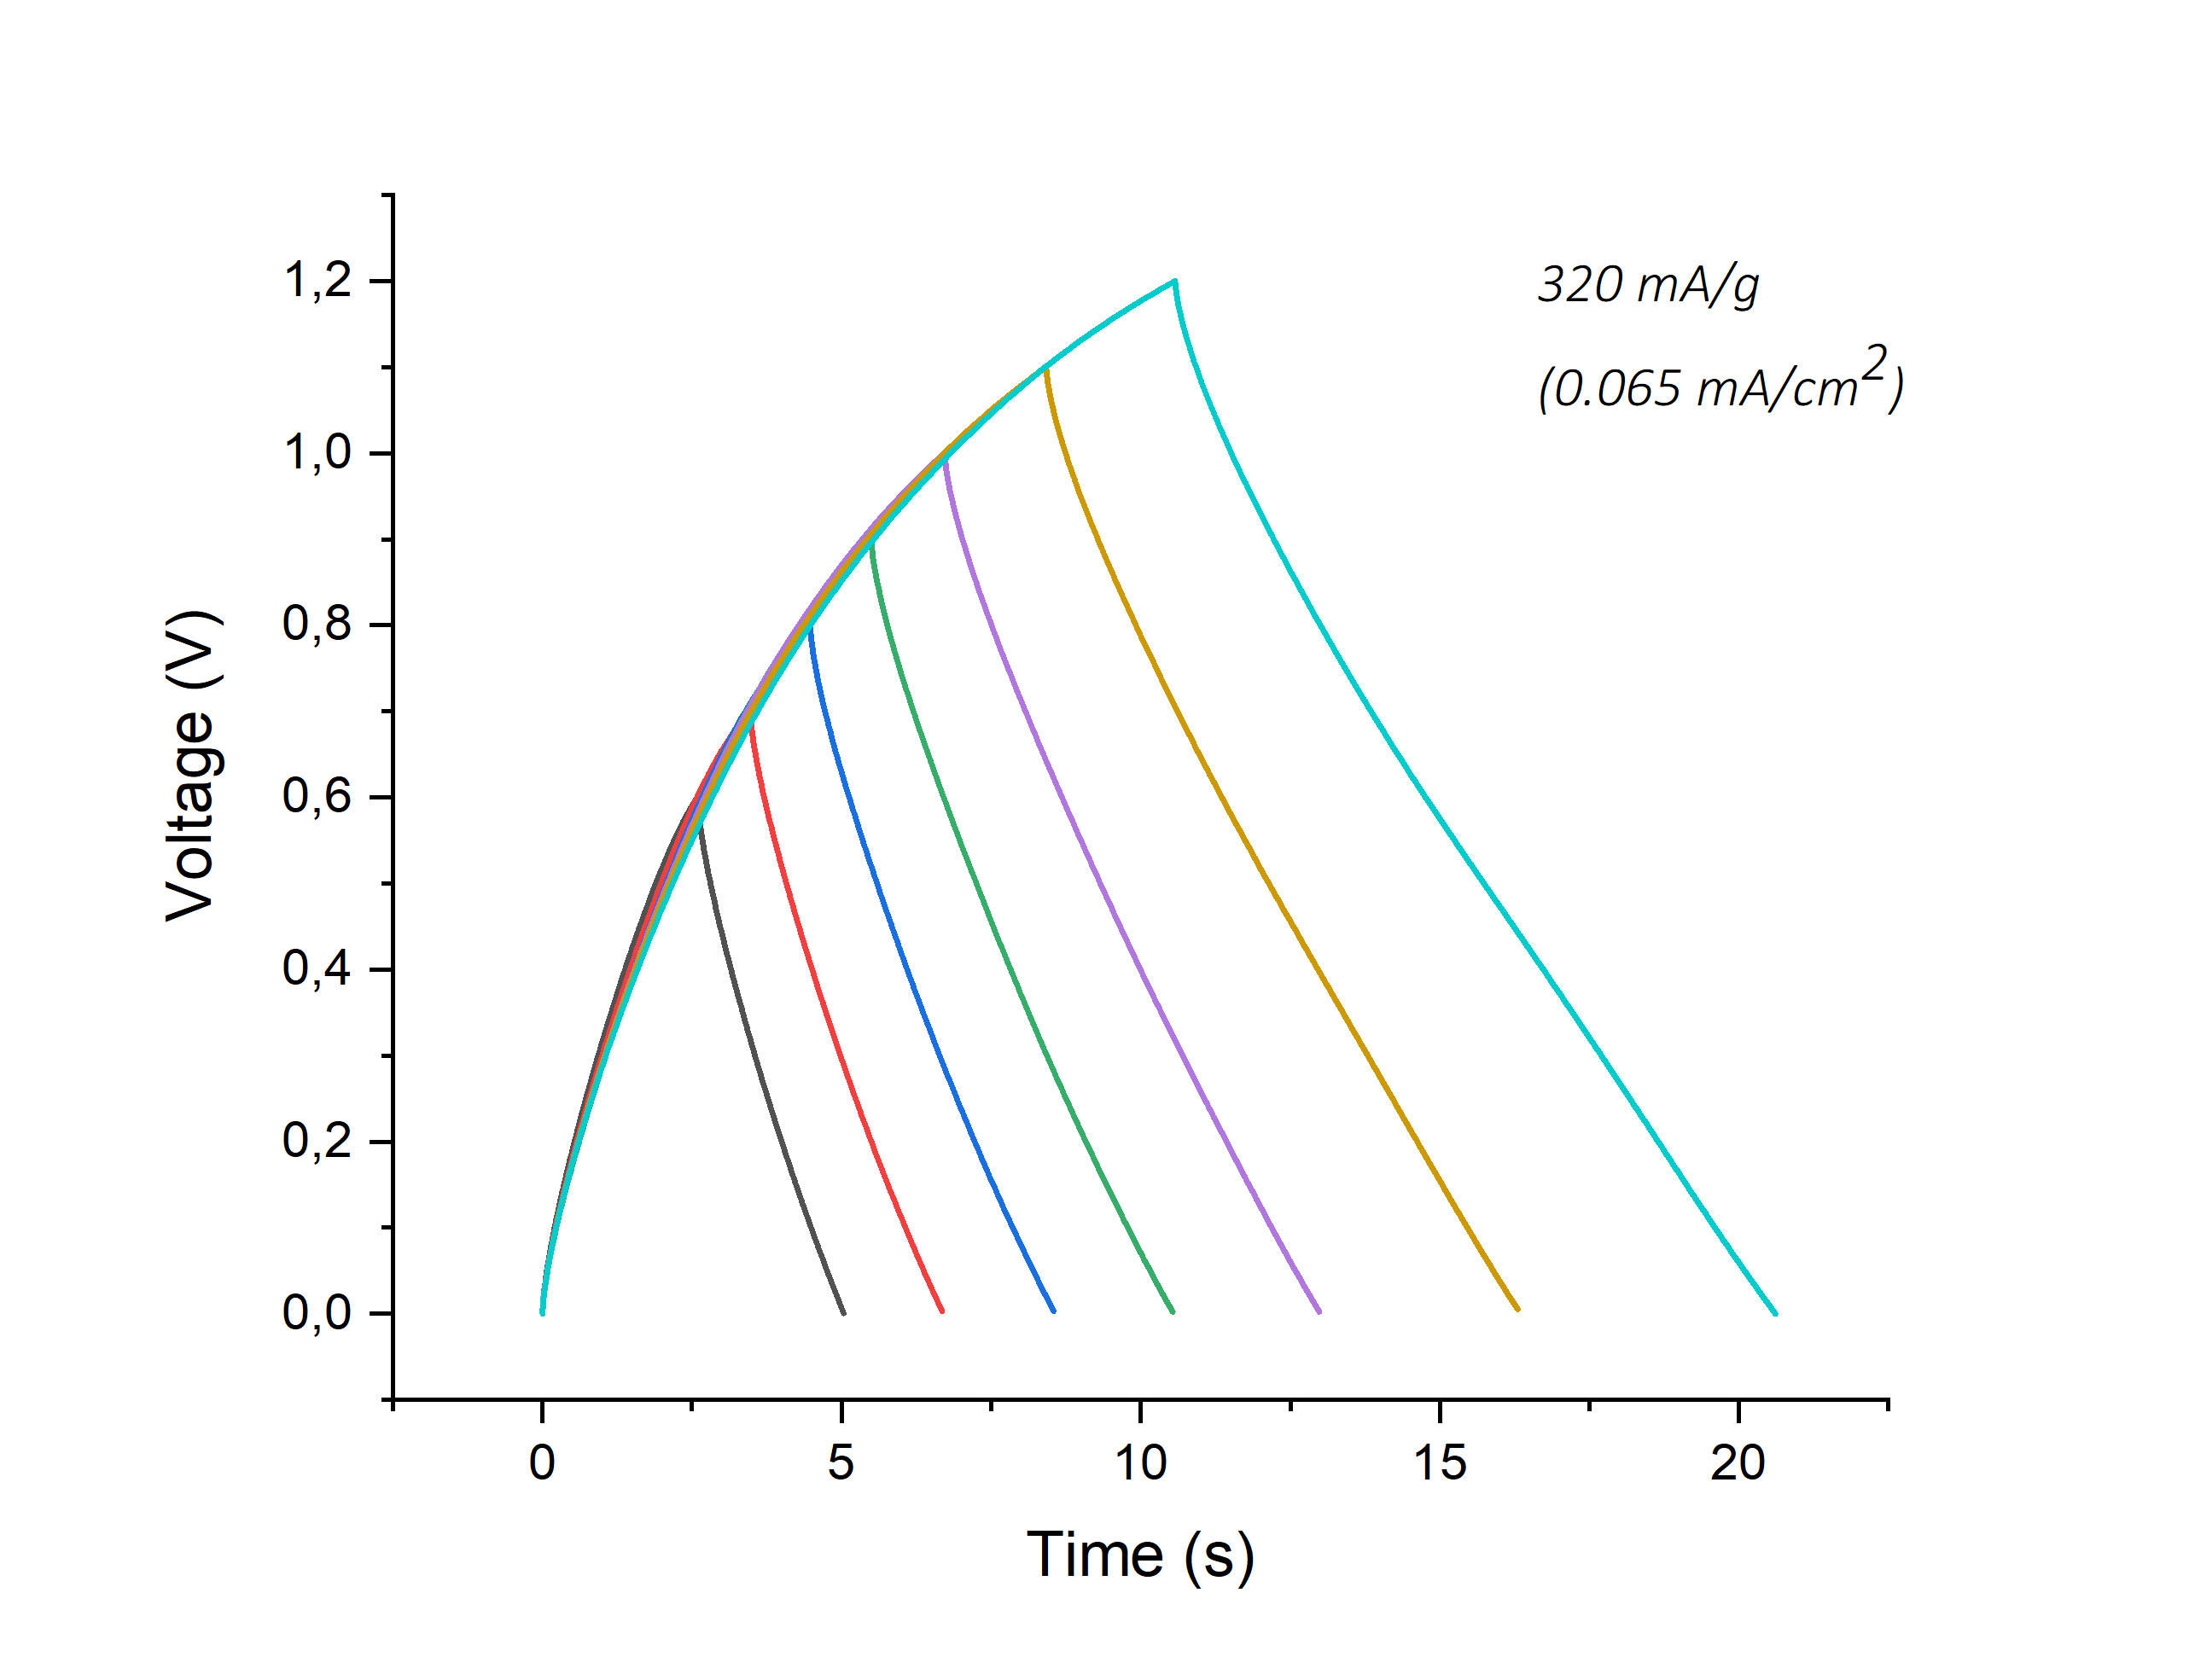
\includegraphics[width=1\textwidth]{Figures/Results/Electrochemistry/LIGP-PI-NaNO3-Swagelok/Cell2/GCPL_Vmax12_cell2_const-current.jpg} 
\captionsetup{width=0.9\linewidth}
\caption{LIGP-Kapton Electrodes, Cell 2. GCPL runs at 320\:mA/g for $V_{max}$ up to 1.2\:V}
\label{fig:LIG-PI-cell2-CC-12}
\end{subfigure}
\begin{subfigure}{0.49\textwidth}
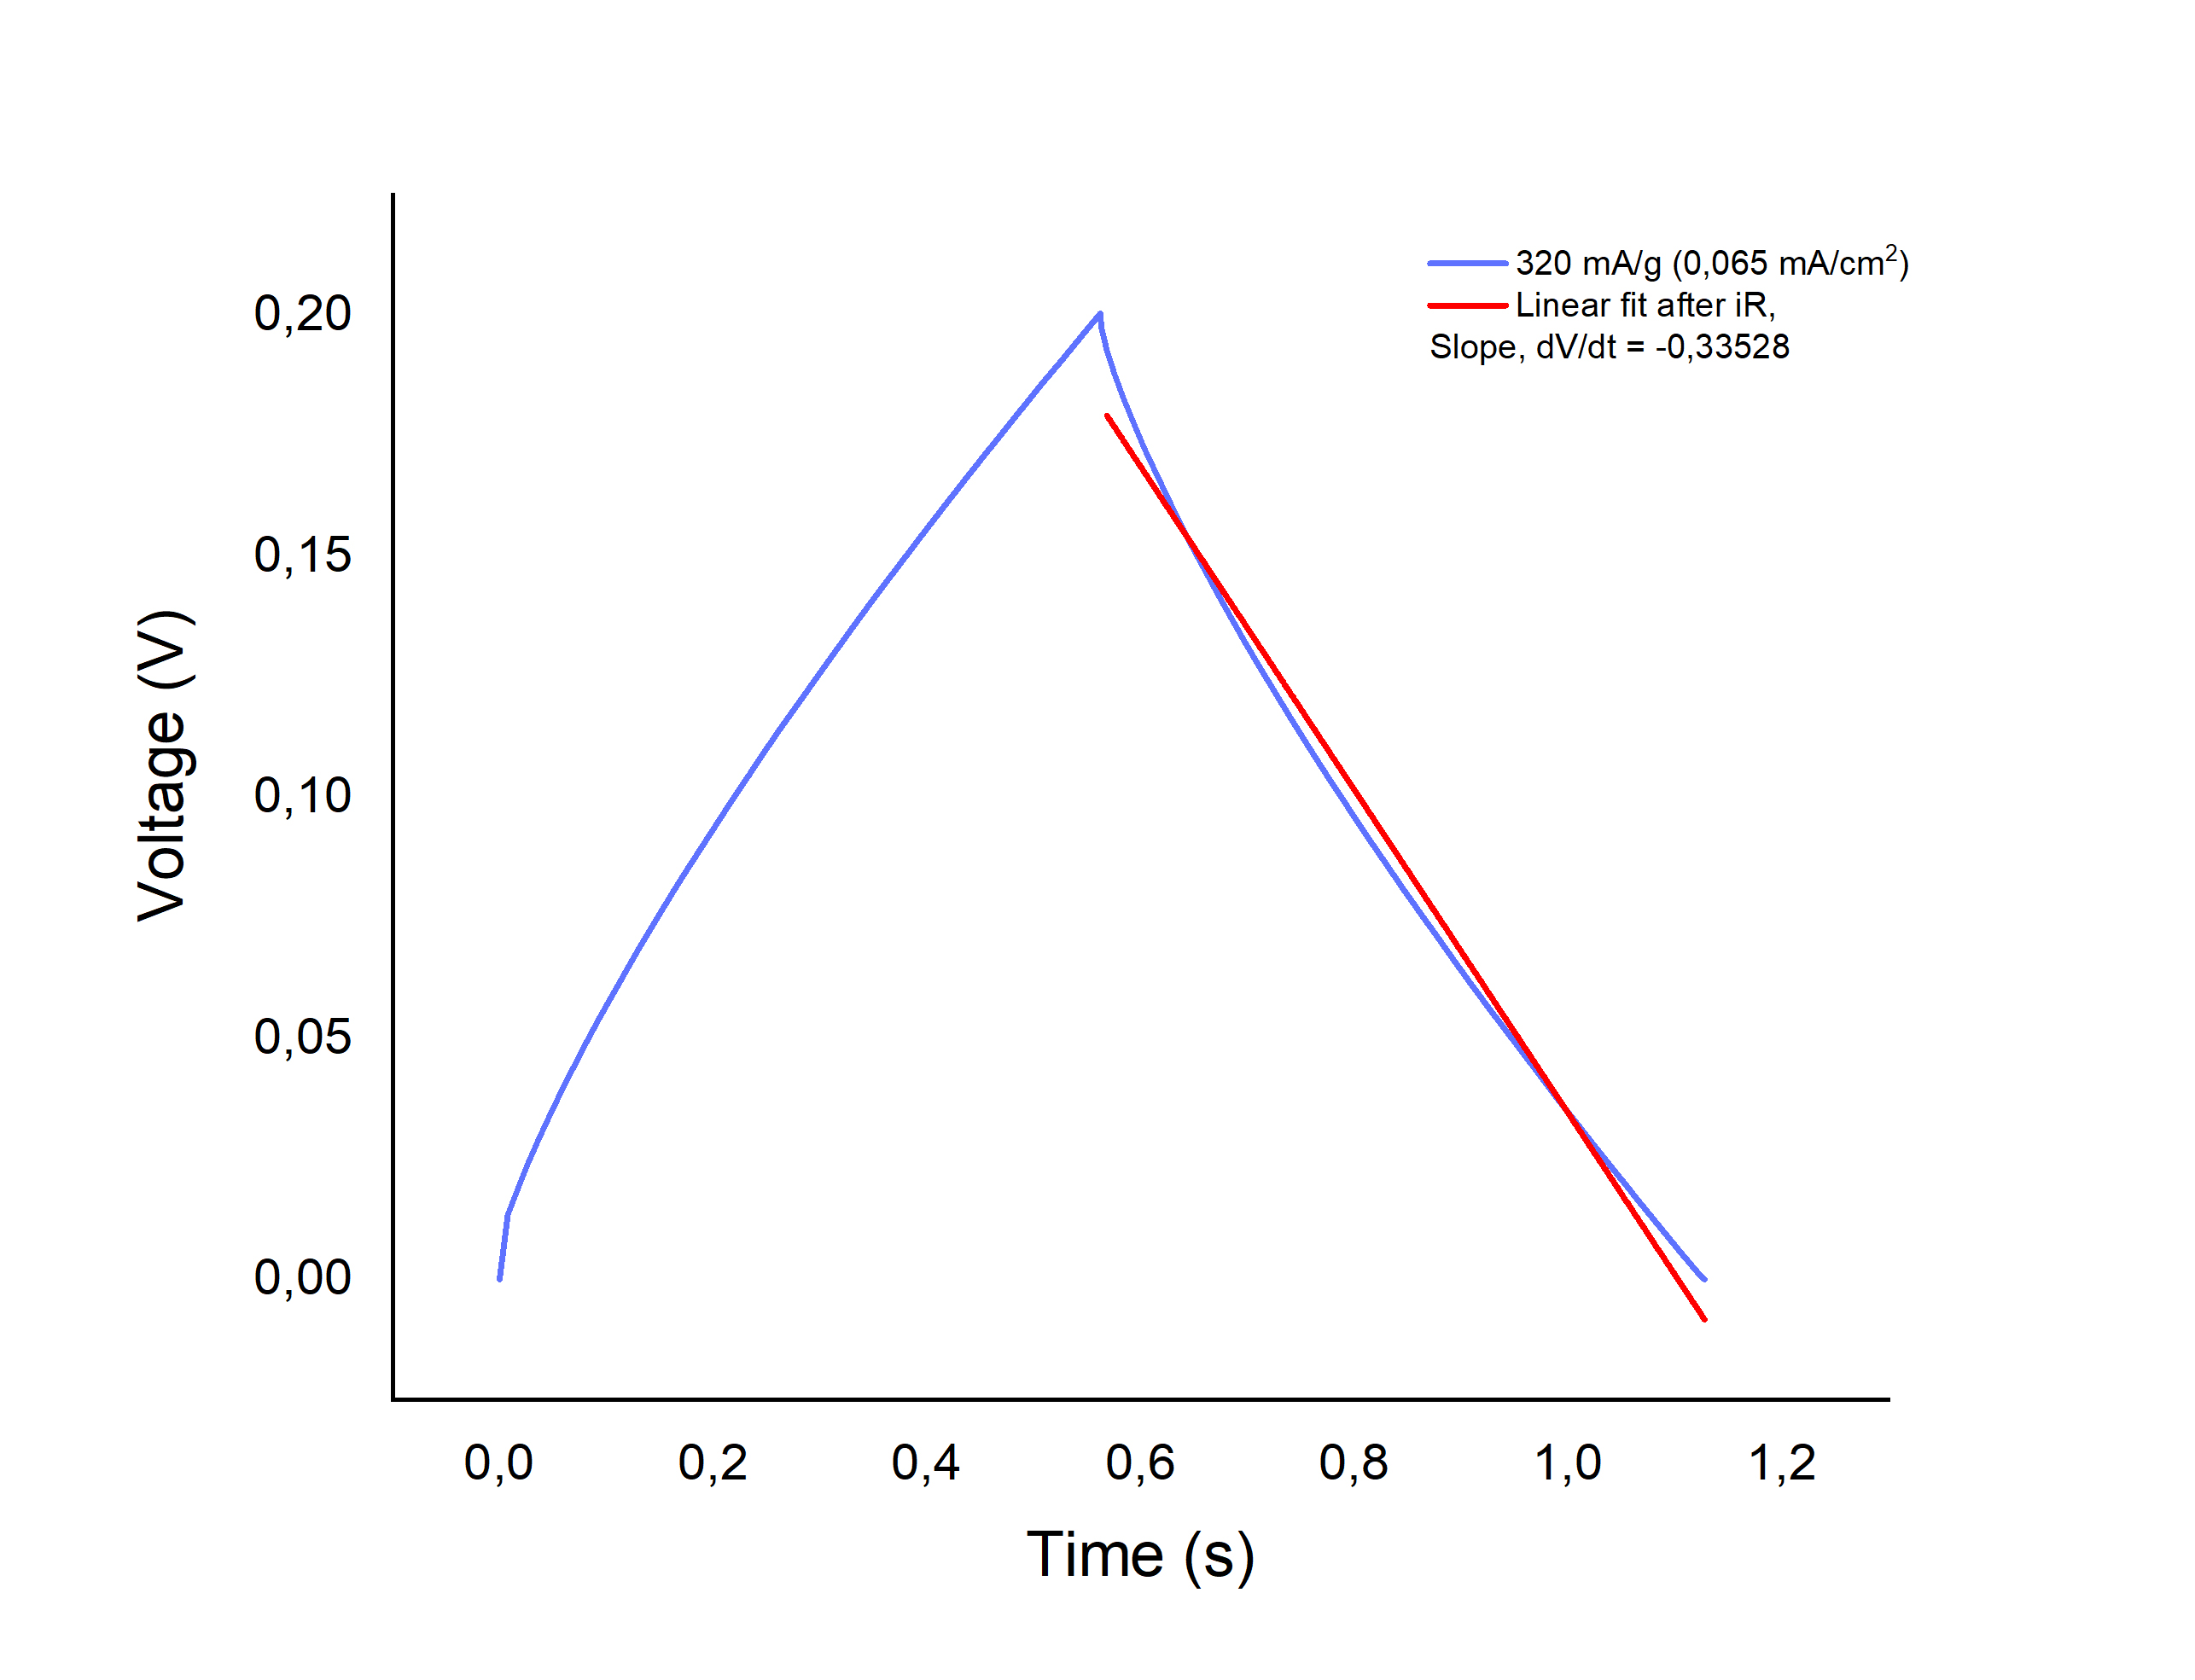
\includegraphics[width=1\textwidth]{Figures/Results/Electrochemistry/LIGP-PI-NaNO3-Swagelok/Cell1/GCPL_Vmax02_cell1_320mA-g-fit.jpg}
\captionsetup{width=0.9\linewidth}
\caption{Towards determination of the slope of a discharge branch of a CC curve for capacitance evaluation}
\label{fig:cc-slope-determination}
\end{subfigure}
\medskip
\caption{CC diagrams of LIGP-Kapton electrodes in Swagelok cells}
\label{fig:LIGP-PI-CC-12}
\end{figure}

For the Cell 1 after tests with higher voltages, the next series of the CV measurements was performed at constant scan rate of 5\:mV/s for lower potentials  $\Delta V$ set to 0.2,\:0.3 ,\:0.4\: and 0.5\:V. These cycles alternated with galvanostatic charge-discharge cycles taking place at 320\:mA/g for $V_{max}$ of 0.2, 0.3, 0.4 and 0.5\:V.

\begin{figure}[H]
\begin{subfigure}{0.49\textwidth}
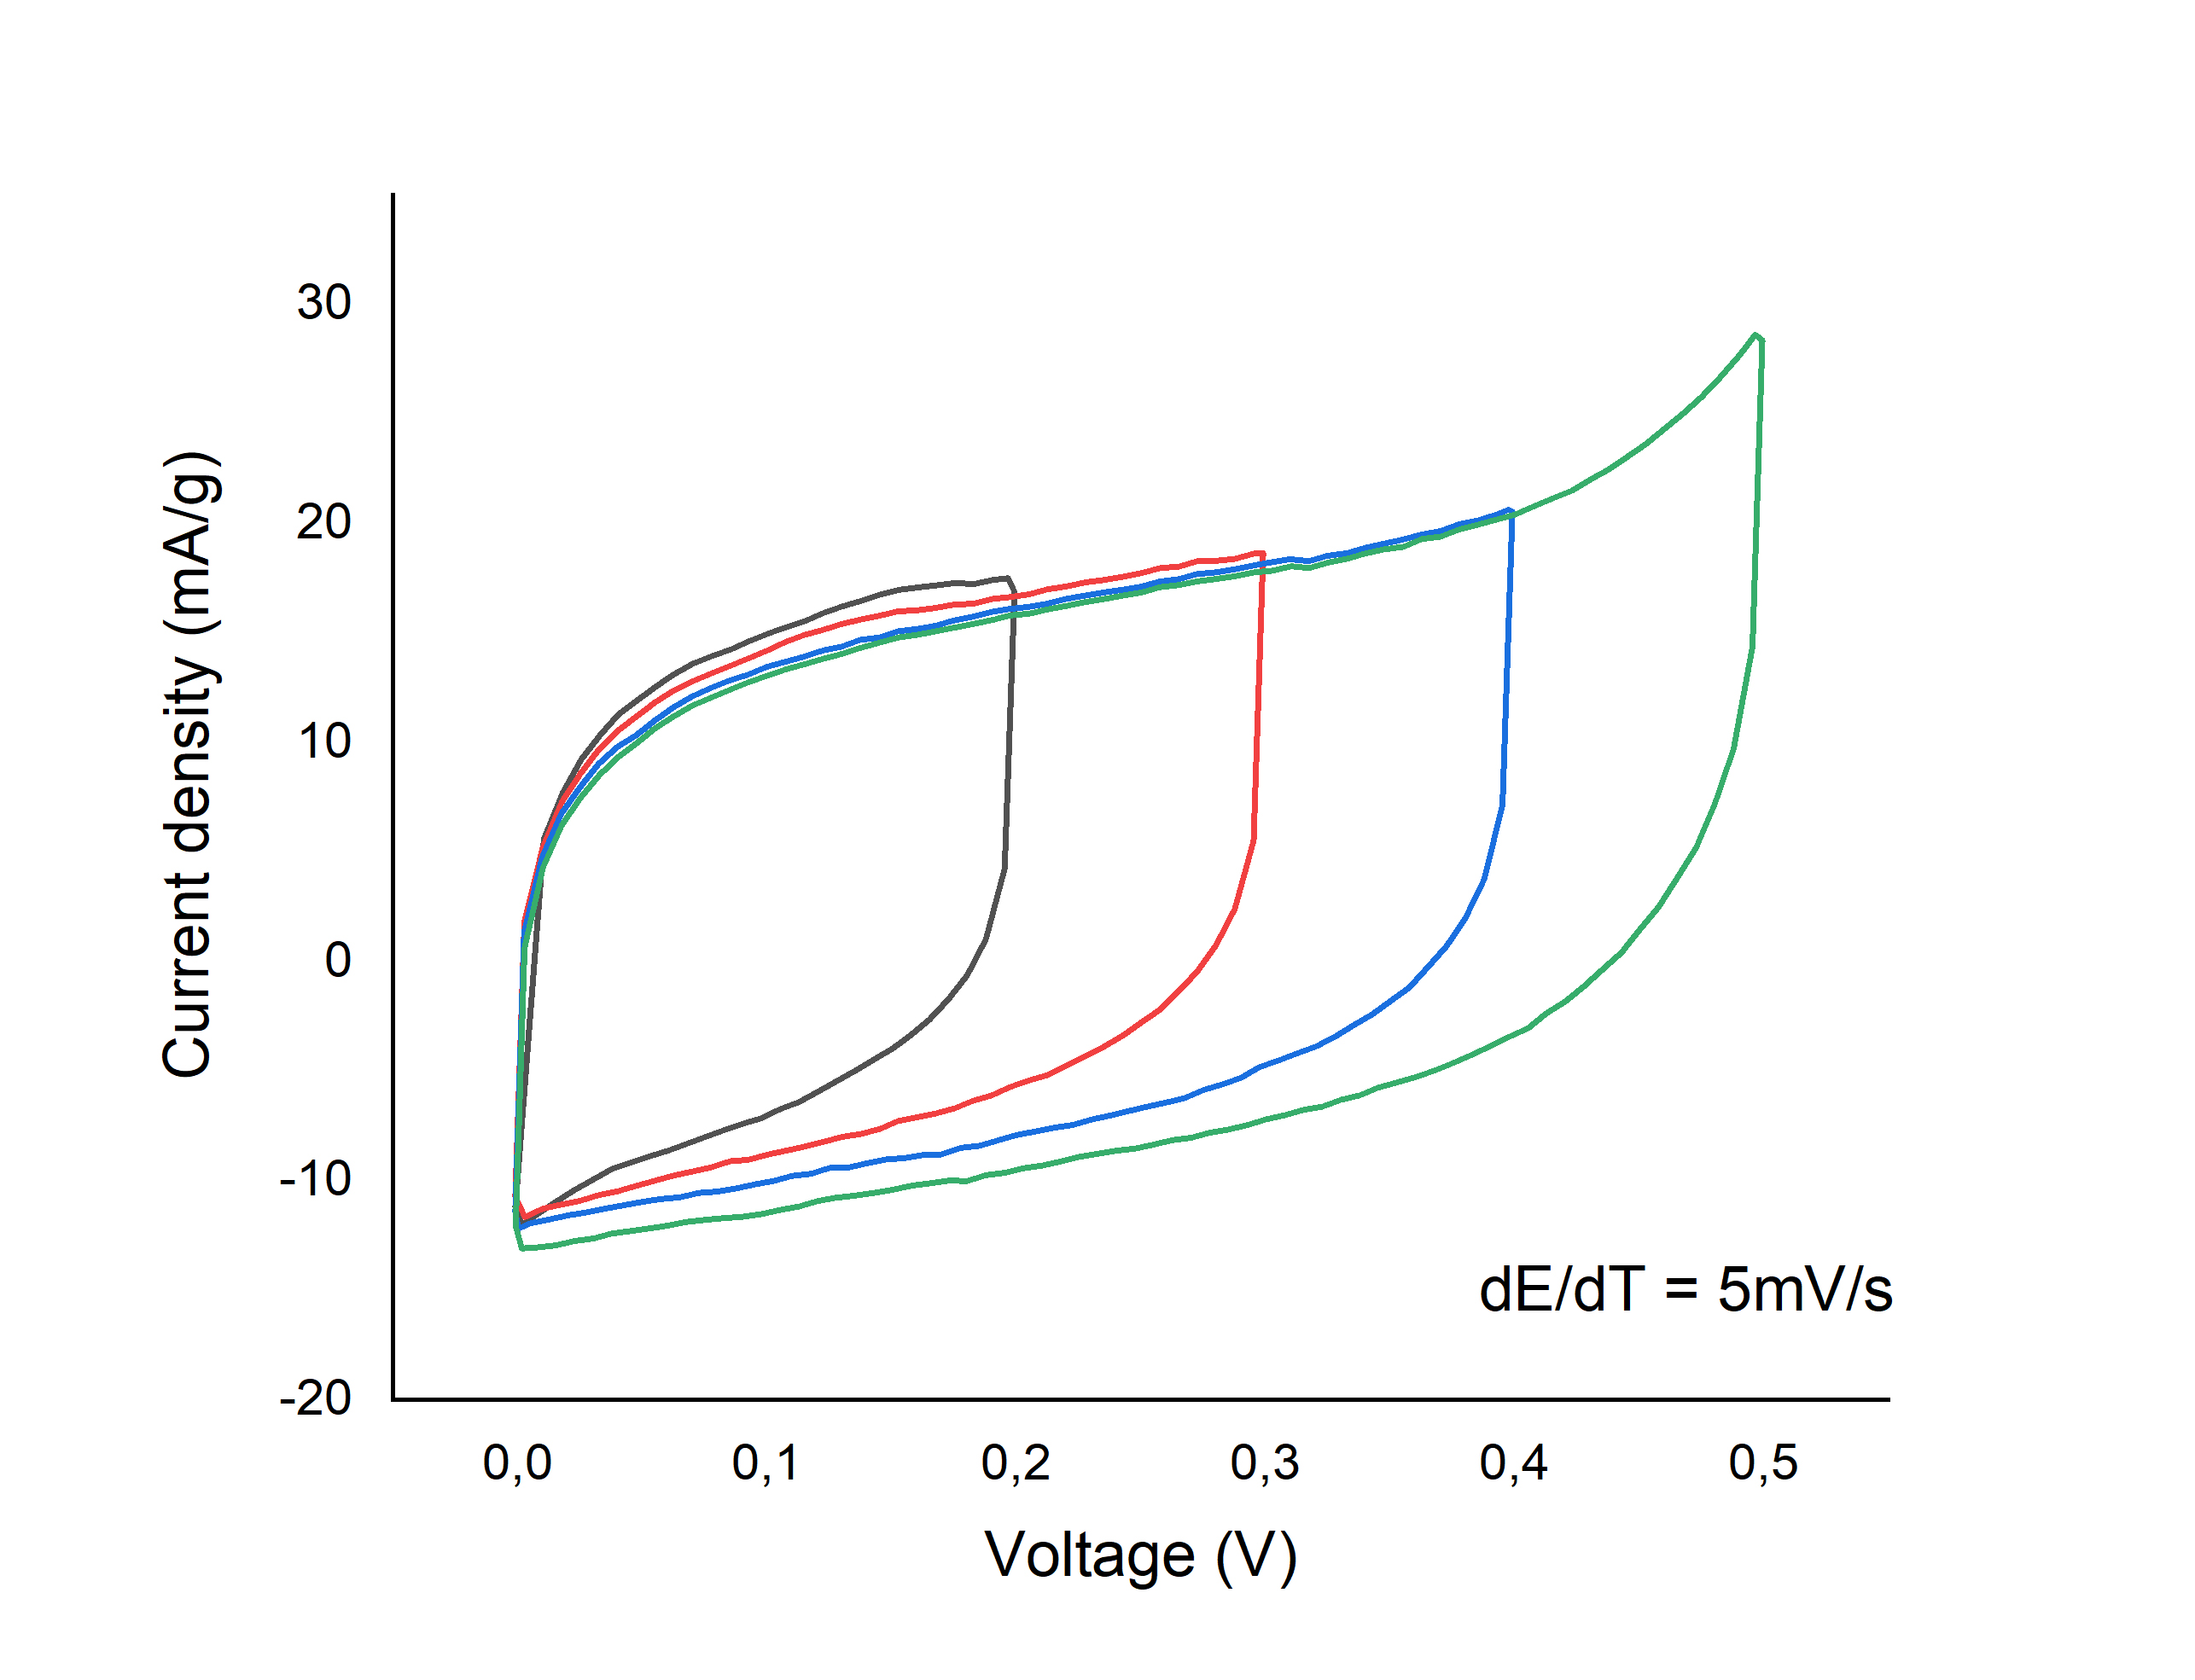
\includegraphics[width=1\textwidth]{Figures/Results/Electrochemistry/LIGP-PI-NaNO3-Swagelok/Cell1/CV-Coming-back-V-06-cell1.jpg} 
\captionsetup{width=0.9\linewidth}
\caption{LIGP-Kapton Electrodes, Cell 1. CV runs at 5\:mV/s for $\Delta V= 0.2 \div 0.5\:V$}
\label{fig:LIG-PI-cell1-CV-06}
\end{subfigure}
\begin{subfigure}{0.49\textwidth}
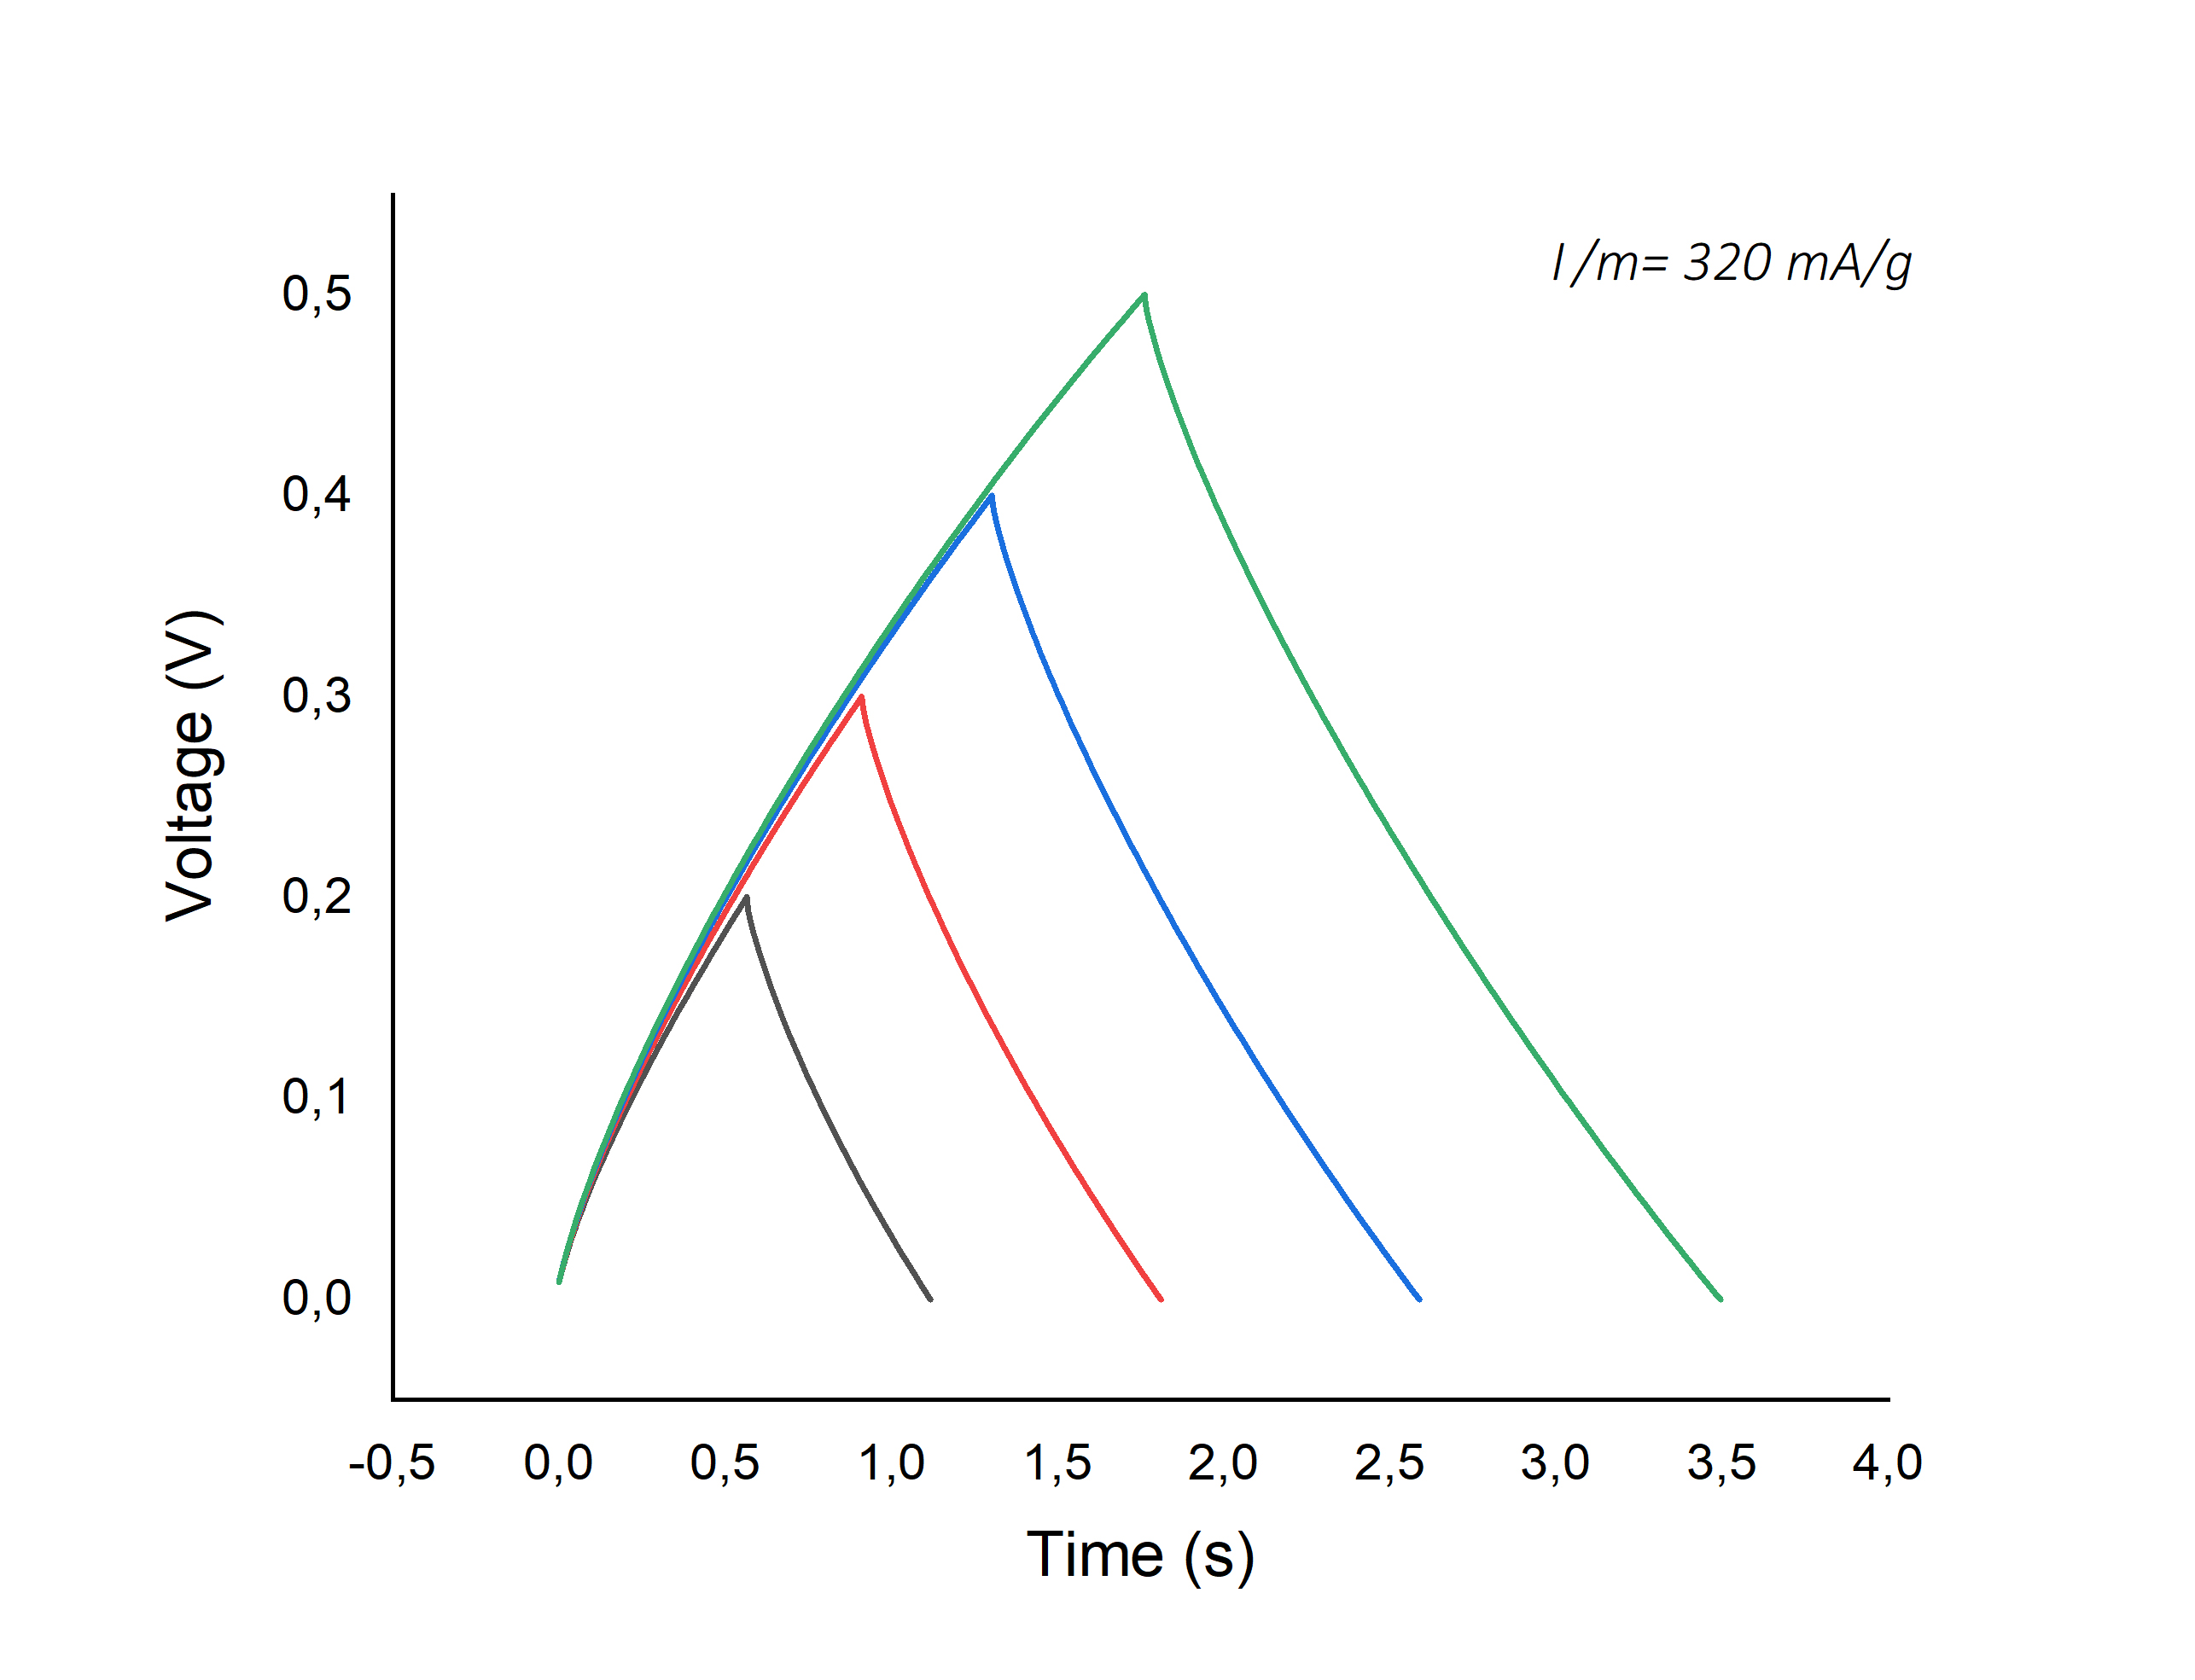
\includegraphics[width=1\textwidth]{Figures/Results/Electrochemistry/LIGP-PI-NaNO3-Swagelok/Cell1/GCPL_Vmax06_cell1_const-current.jpg}
\captionsetup{width=0.9\linewidth}
\caption{LIGP-Kapton Electrodes, Cell 1. CV runs at  320\:mA/g for $V_{max}$ up to 0.6\:V}
\label{fig:LIG-PI-cell1-CC-06}
\end{subfigure}
\medskip
\caption{Constant rate CV and constant current GCPL middle range measurements}
\label{fig:LIG-PI-Cell1-06}
\end{figure}


\textbf{Capacitance Evaluations for LIGP-Kapton Electrodes}

In order to estimate the supercapacitor performance capacitance values were estimated as the main characteristic expressing the ability of a device to store electrical energy. 

Since higher values showed an increasing level of distortion of the rectangular shape of the CV lines, so desirable for supercapacitors, the calculation of the capacitance values $C_g$ and $C_A$ was carried out for the results obtained with smaller voltage ranges up to $\Delta V = 0.5\:V$. The same approach was applied to the GCPL data. The slope value of a discharge CC branch was obtained by a linear fit to the respective curve part straight after the iR drop as shown in Figure \ref{fig:cc-slope-determination}.

The capacitance values calculated with the CV data obtained in the constant voltage window 0 - 0.2 V at stepwise raised $dV/dt$ (Figure \ref{fig:LIGP-PI-CV-02}) have shown a decrease with increasing scan rates. This effect can be attributed diffusion effects taking place for the electrolyte ions, which have more time to penetrate the pores of the electrode material at the lower scan rates, while at higher scan rates the charges only manage accumulate on the outer surface. Figure \ref{fig:LIGP-PI-CV-Capacitance-02} shows the comparison of the calculated $C_g\:[F/g]$ values for both tested LIGP-Kapton Swagelok cells: 

\begin{figure}[H]
\centering
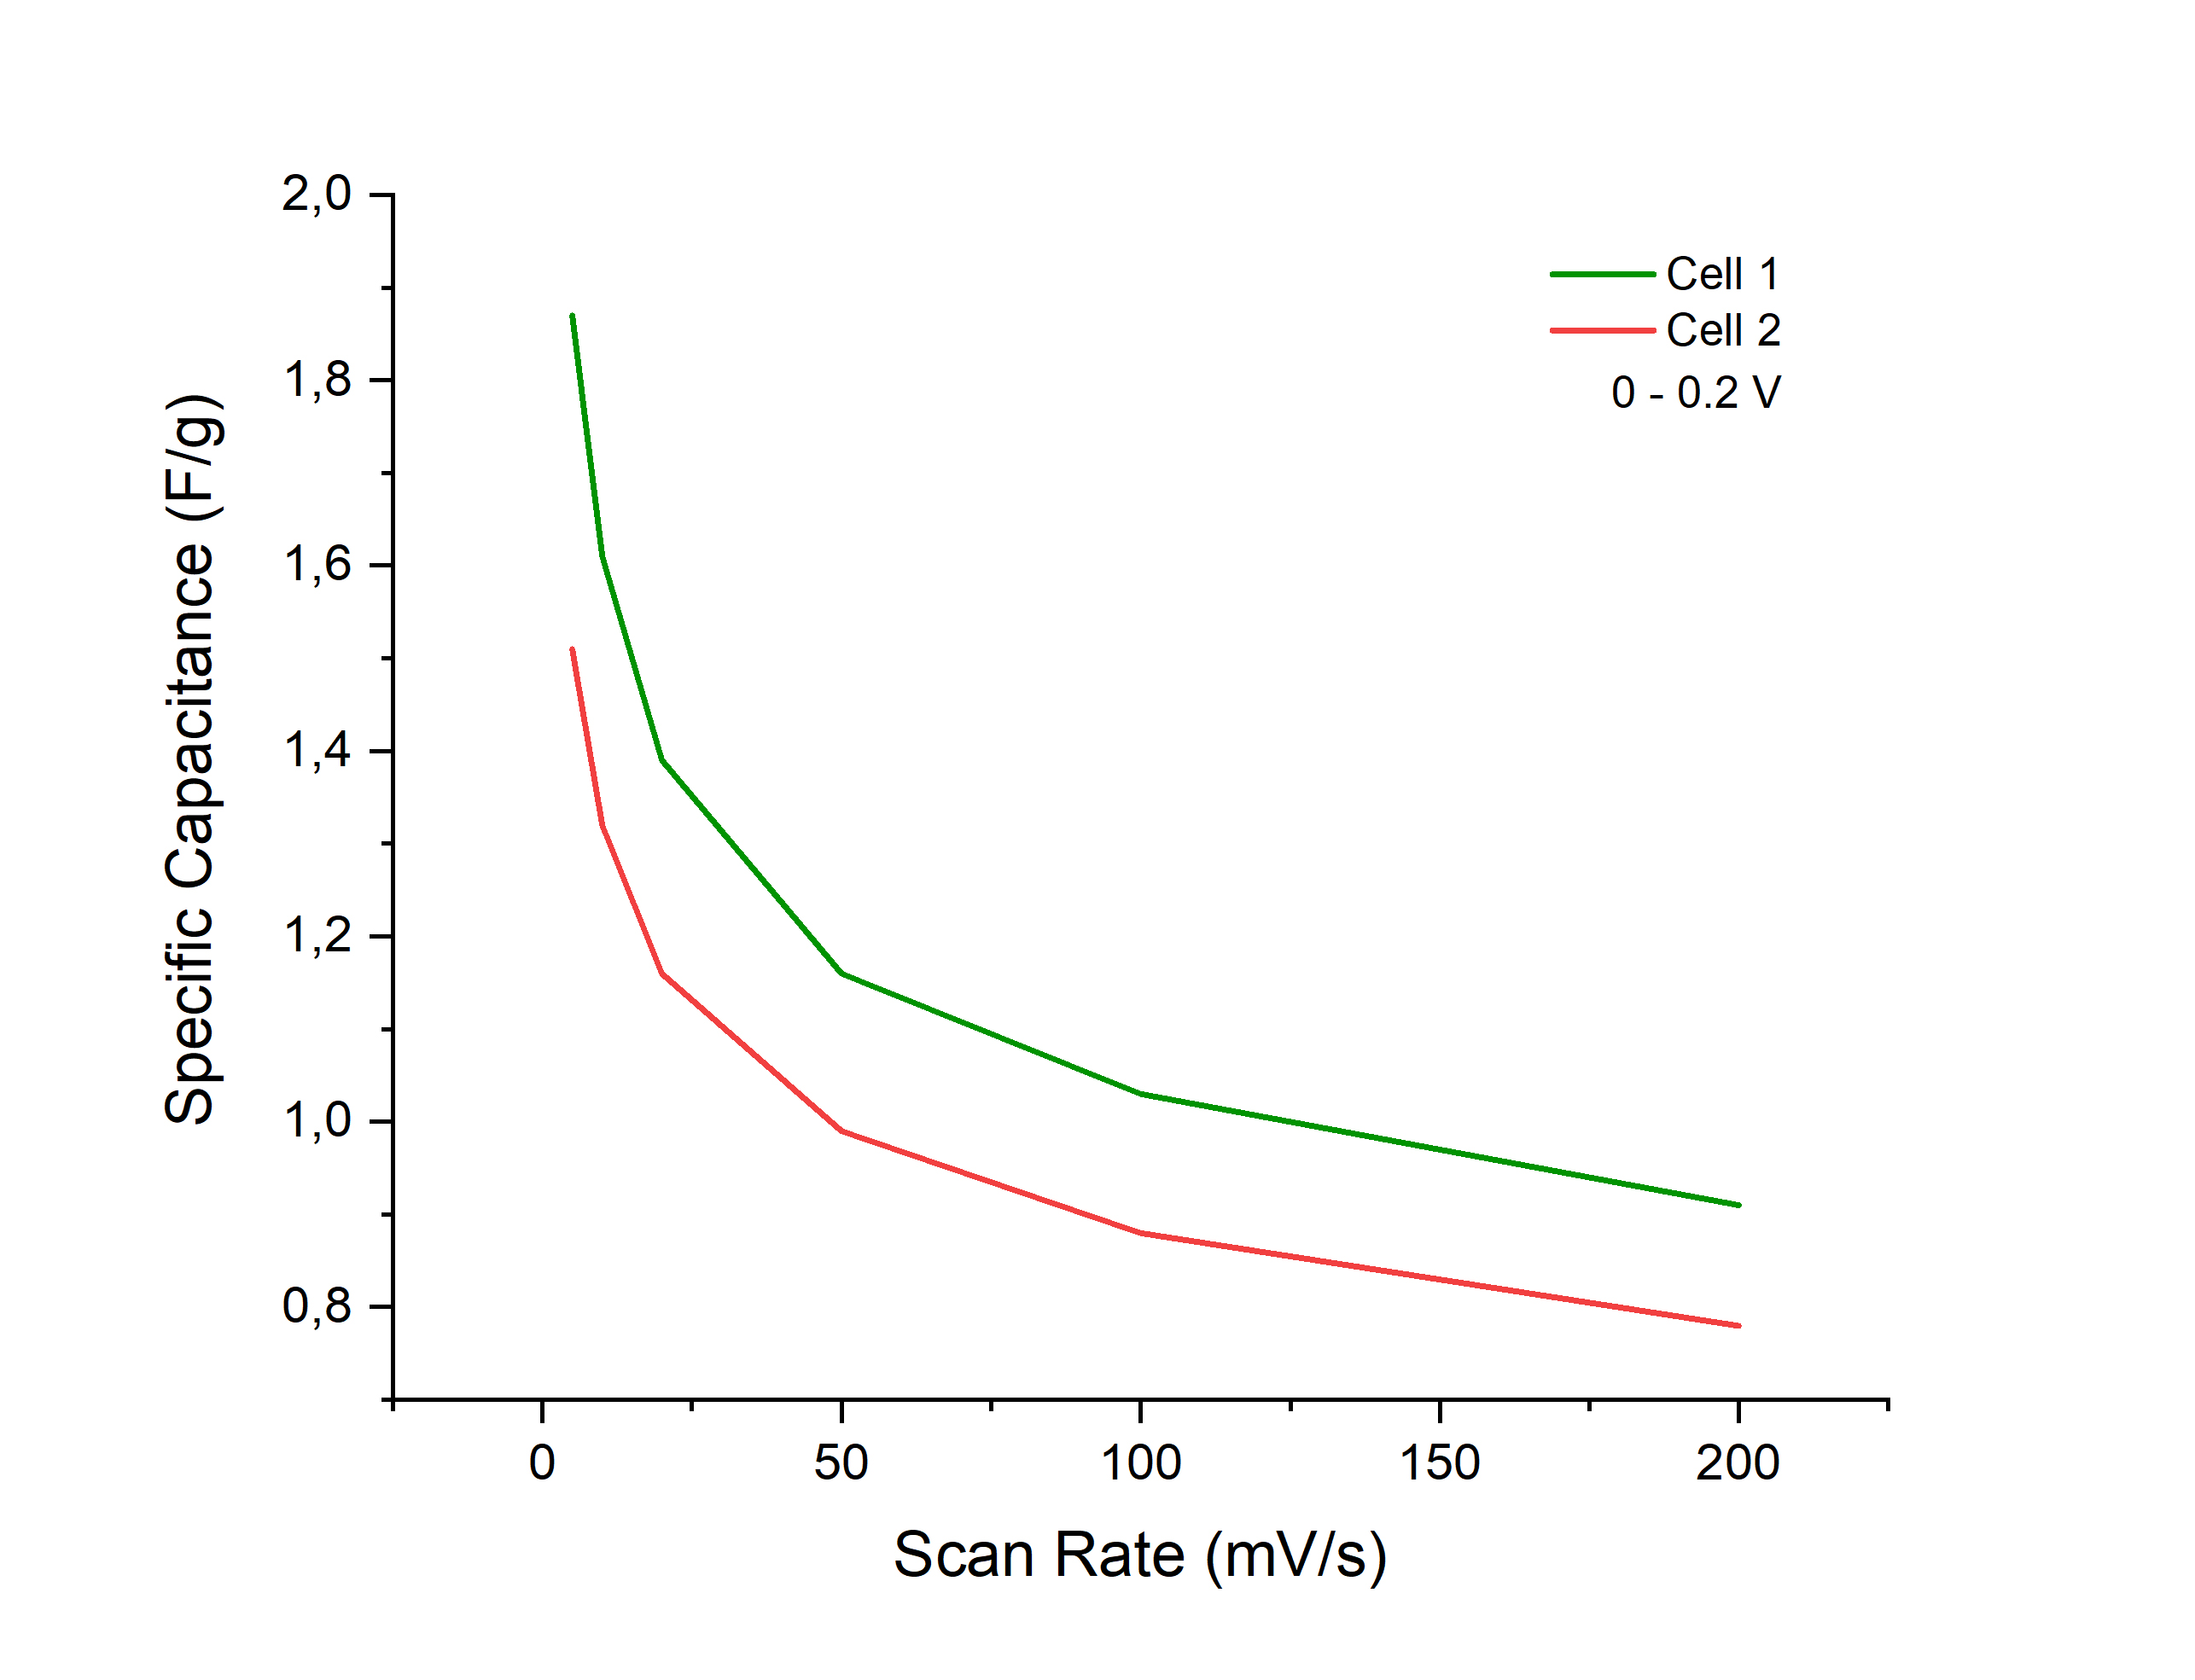
\includegraphics[width=0.5\textwidth]{Figures/Results/Electrochemistry/Comparisons/LIGP-PI-Cells-Comparison-from-CV.jpg}
\medskip
\captionsetup{width=0.7\linewidth}
\caption{LIGP-Kapton specific gravimetric capacitance of Cell\:1 and Cell\:2 evaluated at CV voltage window of 0 - 0.2\:V for increasing scan rates $dV/dt$}
\label{fig:LIGP-PI-CV-Capacitance-02}
\end{figure}

As one can see from Figure \ref{fig:LIGP-PI-CC-02} specific capacitance calculated from CC curves as a function of current density have shown similar tendency, namely the estimated values decreased with an increase of the applied current for $V_{max}$ staying constant at 0.2 V. In this case higher current density values mean faster charge-discharge cycle, which logically leads to the same effect hindering the charges to penetrate the bulk of the porous electrode to be stored at the deeper interface areas. 

Capacitance evaluation for the CV experiments with constant scan rate but an increasing voltage sweep revealed that the $C_g$ and $C_A$ values rise proportionally to the rise of $\Delta V$. Similarly for GPCL data obtained for the applied current staying at 320\:mA/g but with $V_{max}$ increasing stepwise from 0.2 to 0.5\:V it was found that the capacitance increases proportionally to $V_{max}$ and therefore to the total time of a charge-discharge cycle: 

\begin{figure}[H]
\begin{subfigure}{0.49\textwidth}
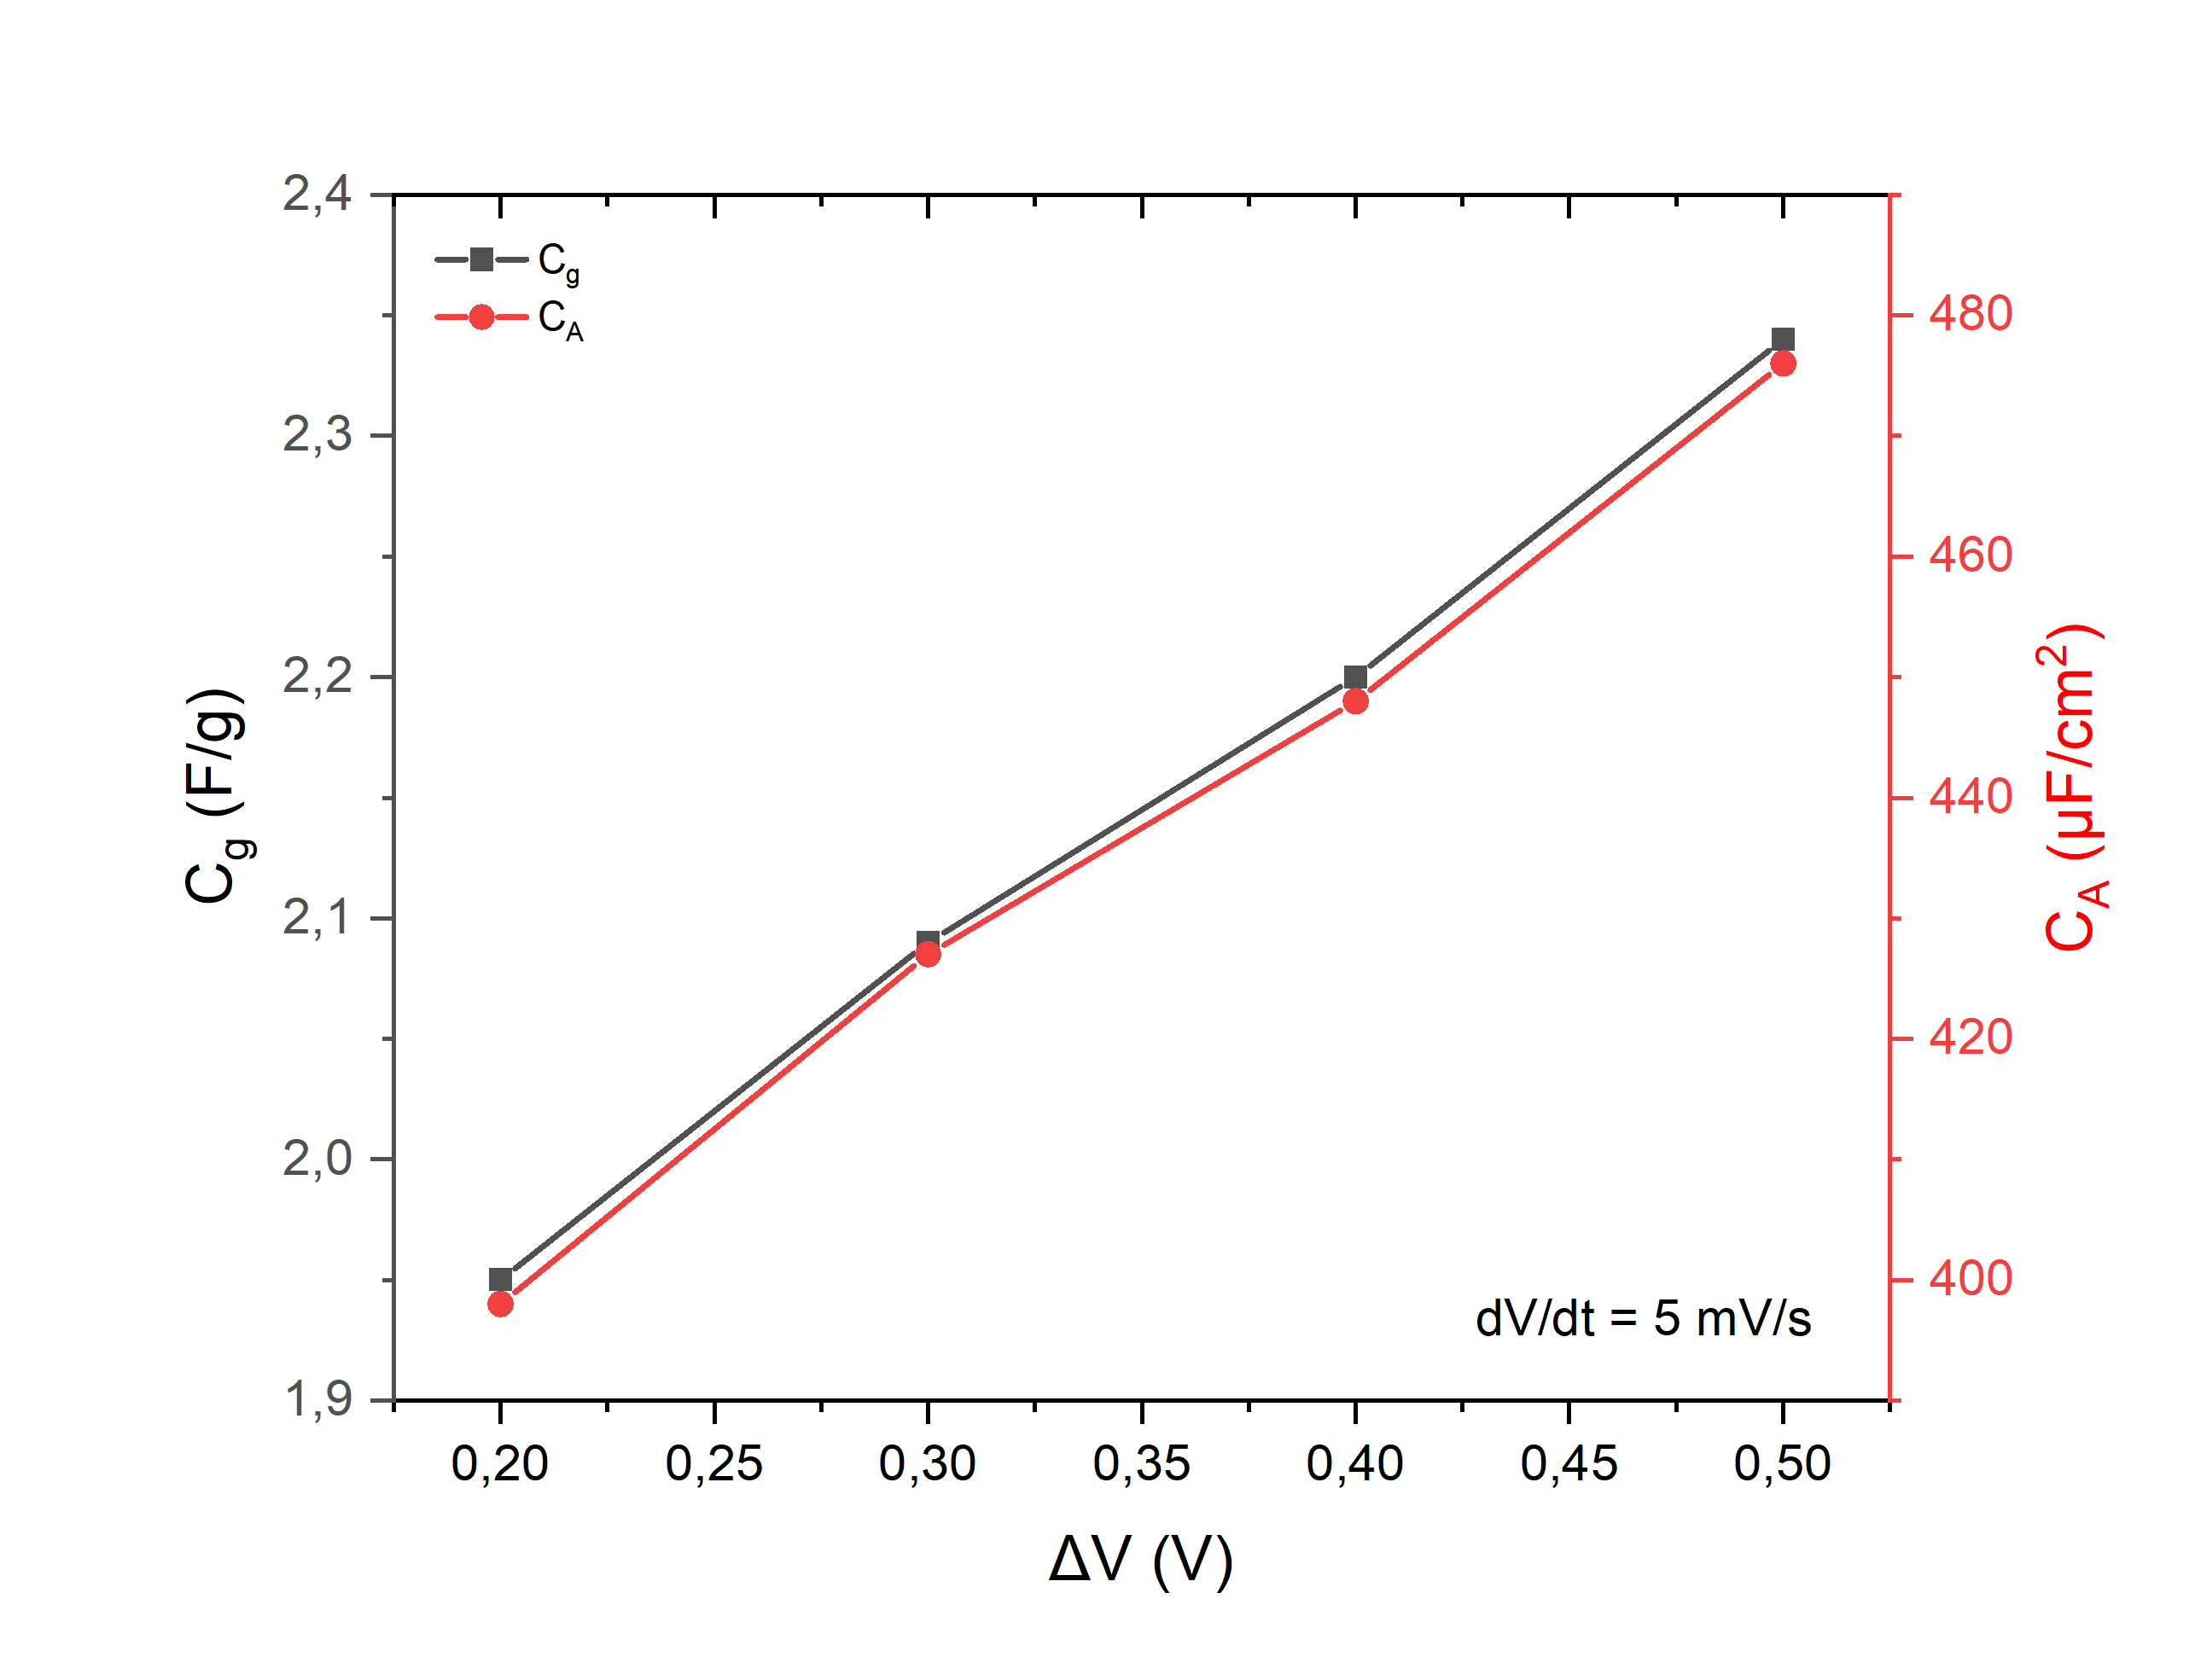
\includegraphics[width=1\textwidth]{Figures/Results/Electrochemistry/Comparisons/Capacitance_const_scan_rate_5.jpg} 
\captionsetup{width=0.9\linewidth}
\caption{LIGP-Kapton Electrodes, Cell 1. Increase of specific capacitance proportional to $\Delta V$ increase at constant scan rate of 5\:mV/s}
\label{fig:LIG-PI-cell1-C-CV-increase}
\end{subfigure}
\begin{subfigure}{0.49\textwidth}
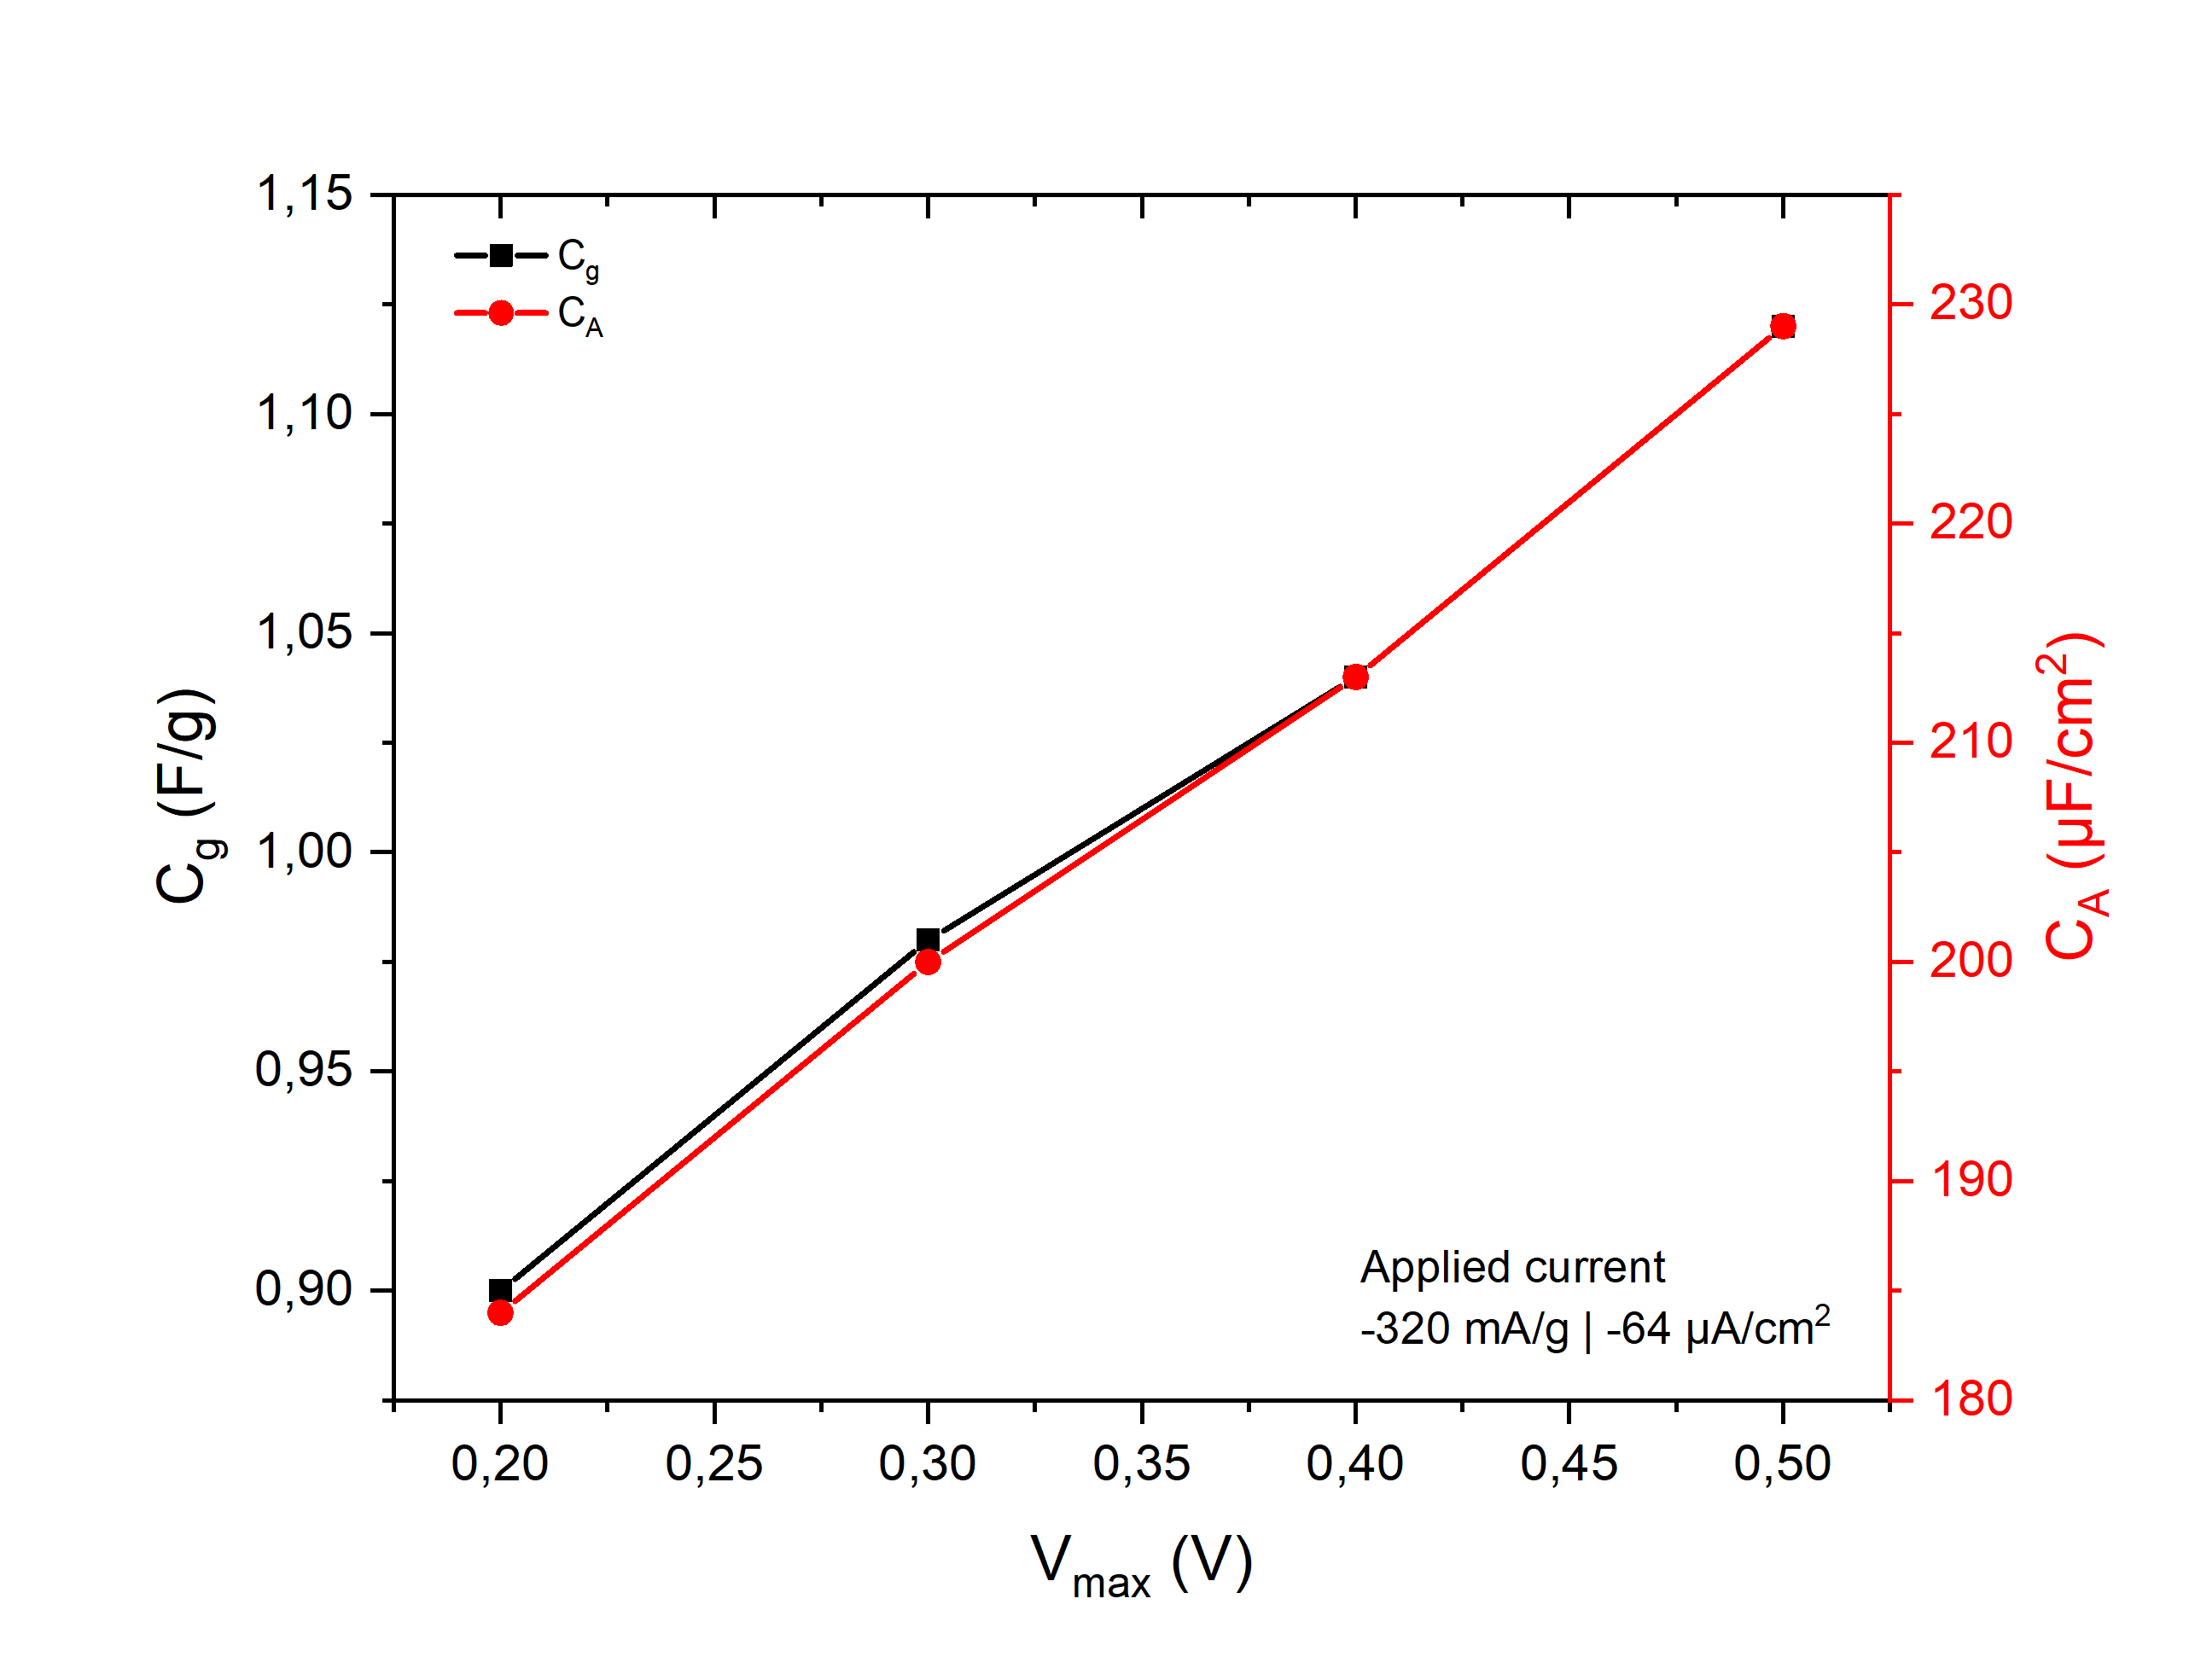
\includegraphics[width=1\textwidth]{Figures/Results/Electrochemistry/Comparisons/Capacitance_const_current_320.jpg}
\captionsetup{width=0.9\linewidth}
\caption{LIGP-Kapton Electrodes, Cell 1. Increase of specific capacitance proportional to $V_{max}$ increase at constant current of  320\:mA/s}
\label{fig:LIG-PI-cell1-C-CC-increase}
\end{subfigure}
\medskip
\caption{Specific Capacitance of LIGP-Kapton electrode evaluated with CV and GCPL data}
\label{fig:LIG-PI-cell1-C-increase}
\end{figure}

\textbf{LIGF on Kapton Electrodes in a Swagelok Cell}

The next variation of electrode to be tested was LIGF on Kapton (Type 2 in the Table \ref{tab:supercapacitor_electrodes} above). Two Swagelok cells with 1M NaNO$_3$ as an electrolyte were prepared. However the Cell 1 had shown poor performance already in the preliminary CV runs which indicated too high inner resistance, probably due to a failure of the VIA contacts, and so it was not tested in the following electrochemical experiments. 

For Cell 2, the first stage of measurements was carried out according to protocols similar to those used for the LIGP-Kapton electrodes described earlier. Figure \ref{fig:LIGF-PI-cell2-CV02} presents nearly perfect rectangular shape of the resulted CV curves at a constant voltage window at 0 - 0.2 for stepwise increased scan rate. However as it can be seen from this Figure the current densities that were achieved were about an order of magnitude smaller than those of LIGP-Kapton electrodes. After the cyclic voltammetry the GCPL runs for different charge-discharge currents from 100 to 2000\:mA/g were performed for the $V_{max}$ fixed at 0.2 V as shown in Figure \ref{fig:LIGF-PI-cell2-CC02}:

\begin{figure}[H]
\begin{subfigure}{0.49\textwidth}
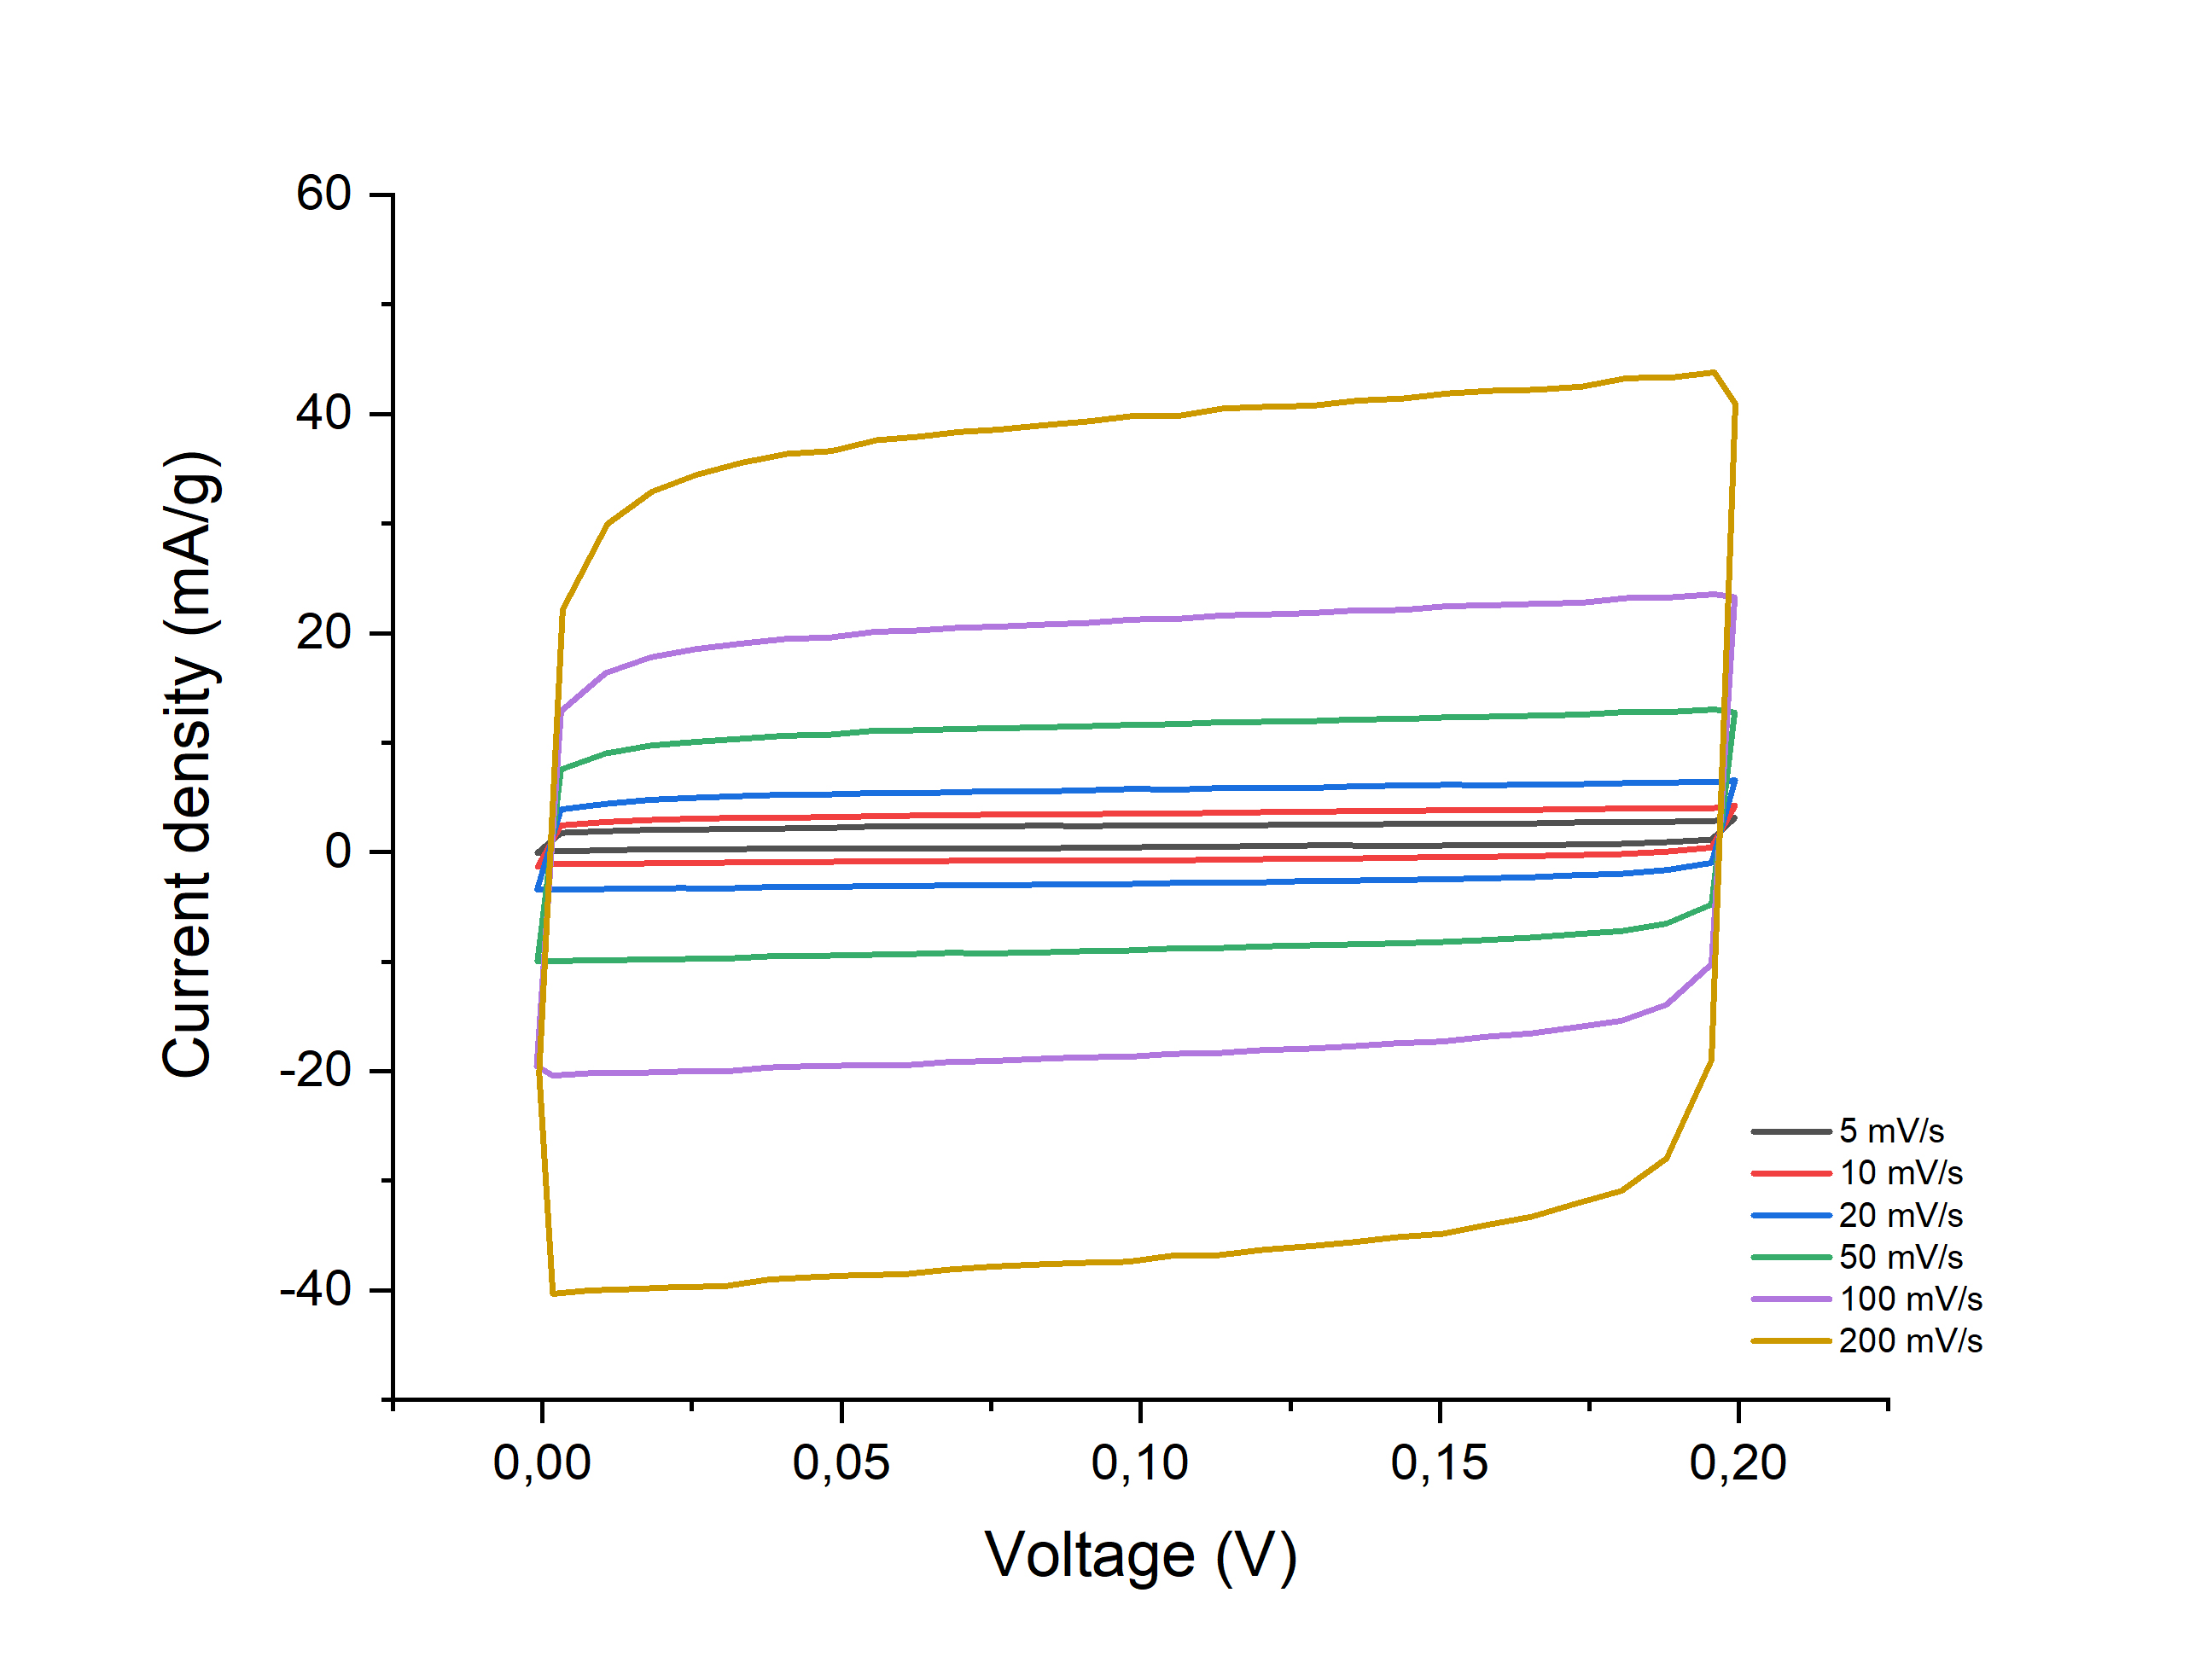
\includegraphics[width=1\textwidth]{Figures/Results/Electrochemistry/LIGF-PI-NaNO3-Swagelok/Cell2/CV-V02-Cell2.jpg} 
\captionsetup{width=0.9\linewidth}
\caption{CV diagrams at 0 - 0.2 V potential window at different scan rates}
\label{fig:LIGF-PI-cell2-CV02}
\end{subfigure}
\begin{subfigure}{0.49\textwidth}
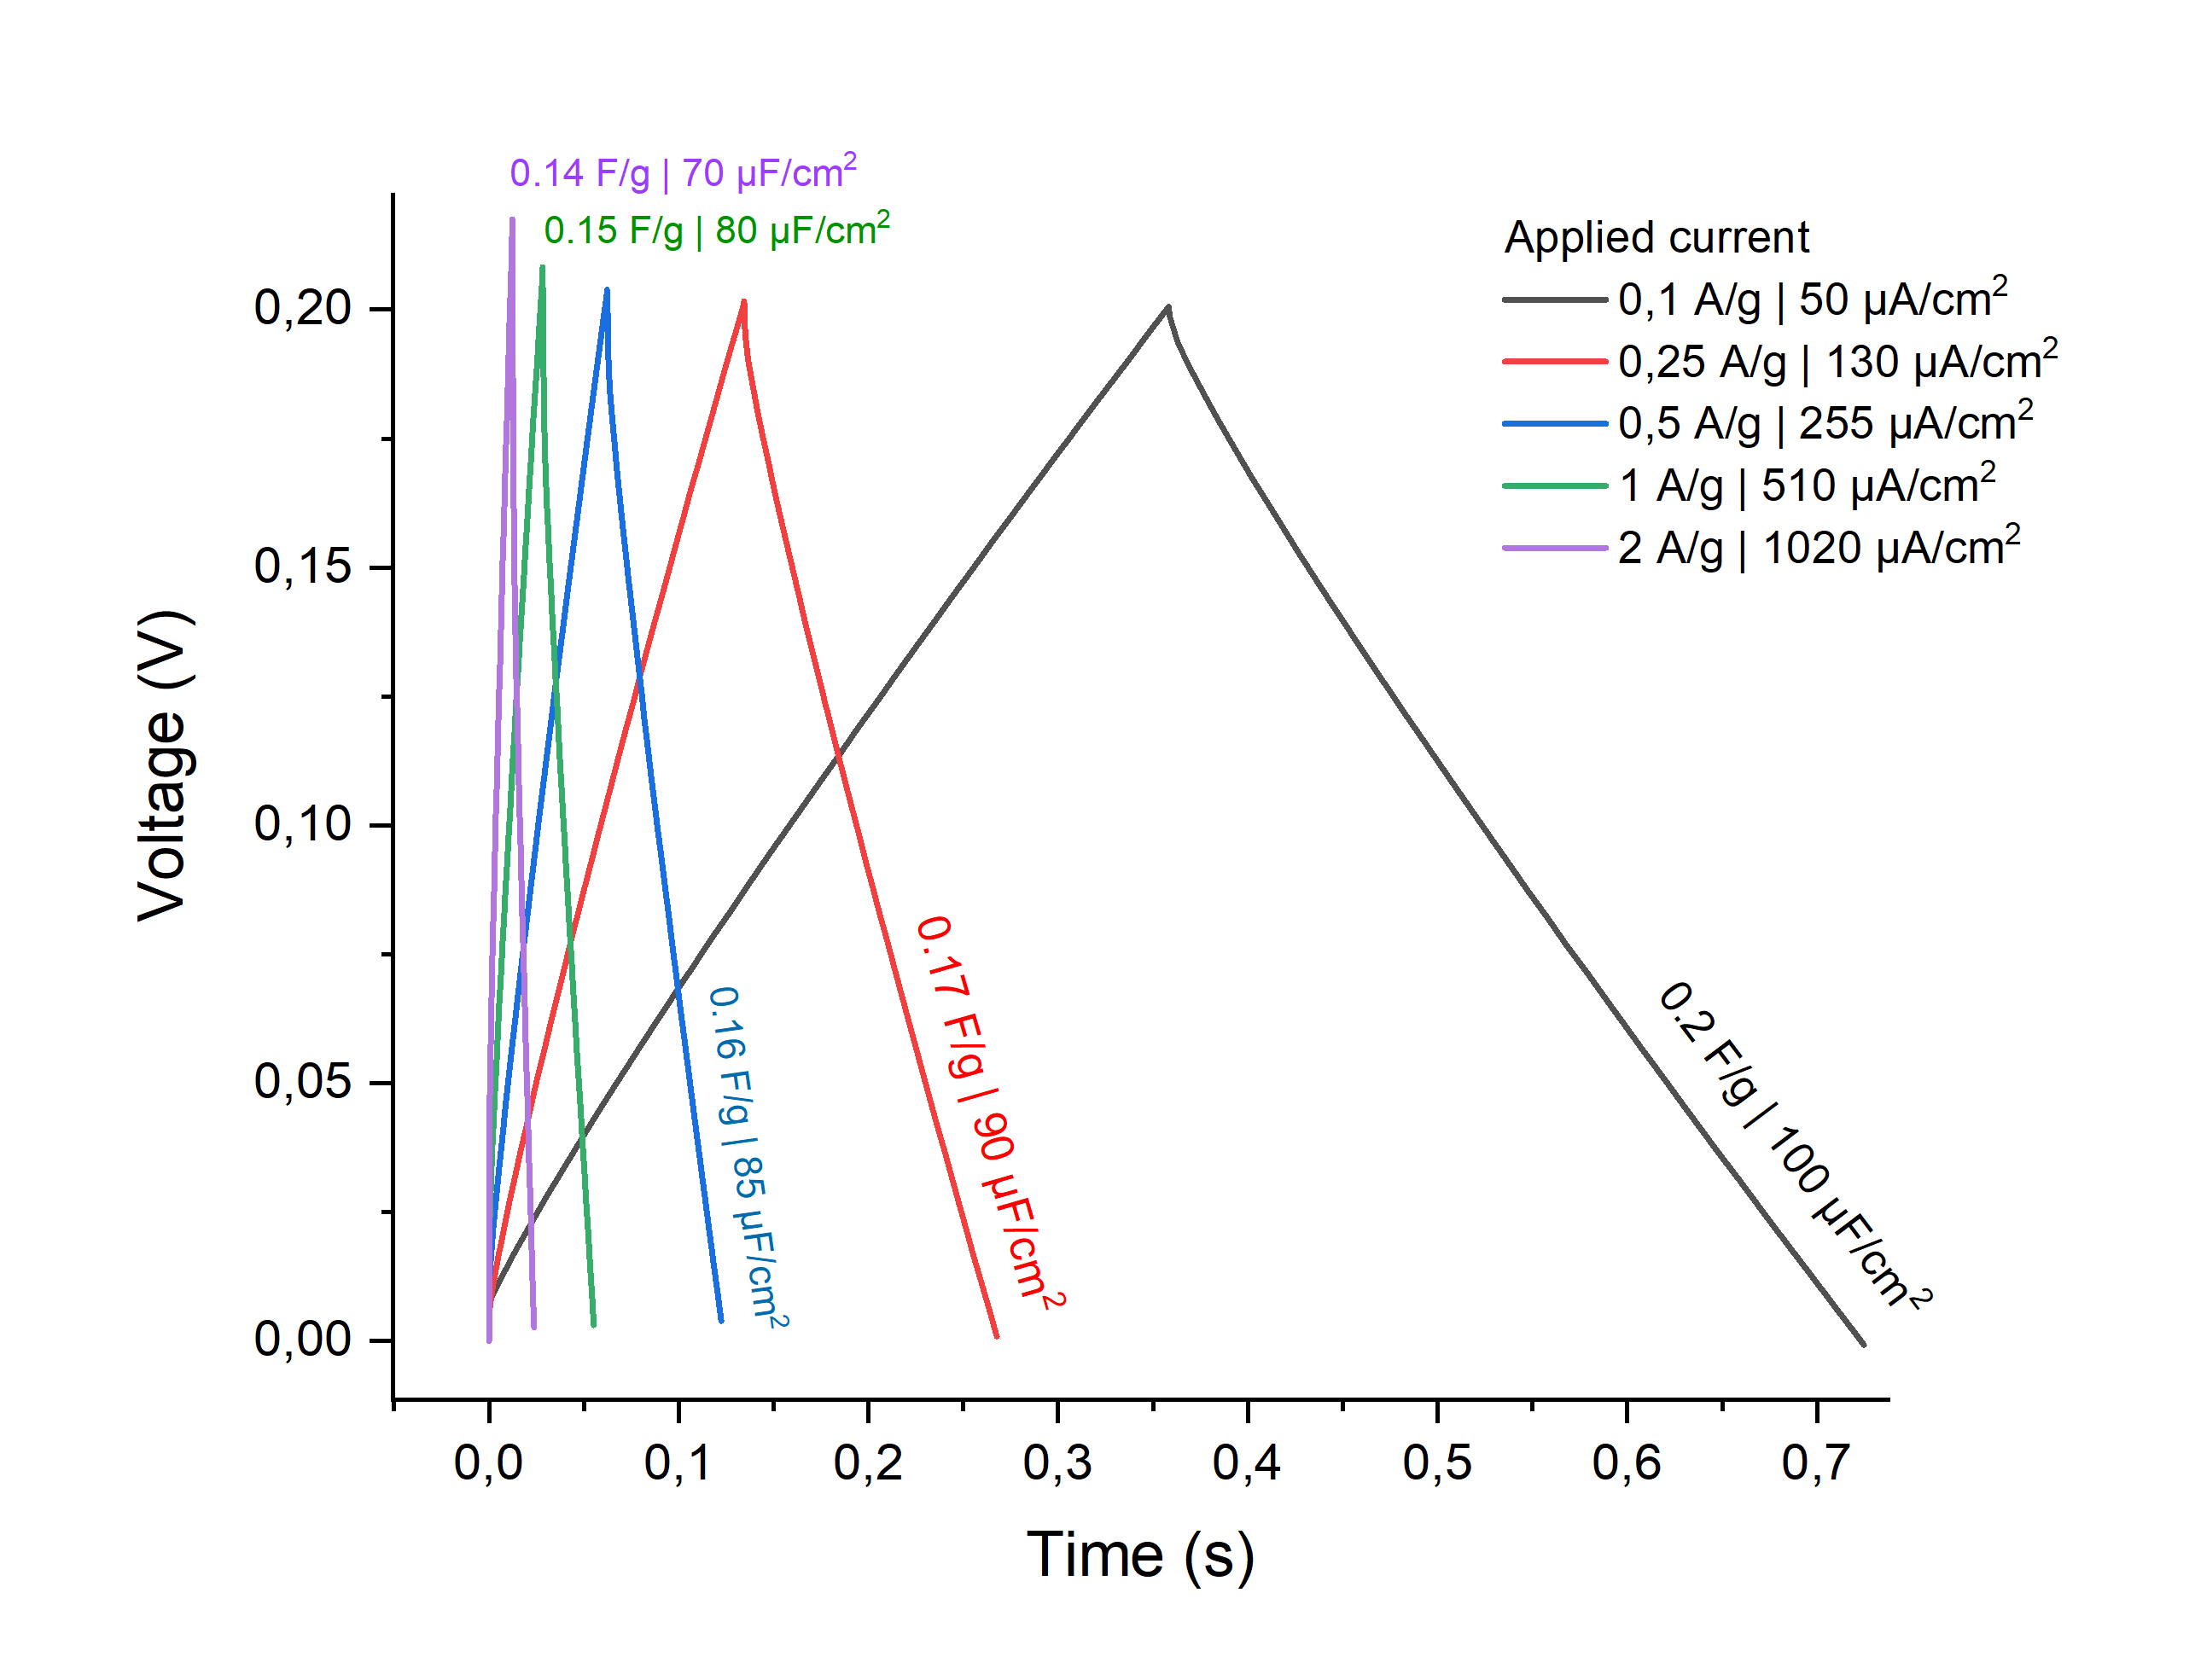
\includegraphics[width=1\textwidth]{Figures/Results/Electrochemistry/LIGF-PI-NaNO3-Swagelok/Cell2/GCPL-V02-Cell2-Cs.jpg}
\captionsetup{width=0.9\linewidth}
\caption{CC diagrams for $V_{max}$=0.2 V at various current densities}
\label{fig:LIGF-PI-cell2-CC02}
\end{subfigure}
\medskip
\caption{LIGF-Kapton Electrodes, Cell 2. CV and GCPL data in the low voltage range 0 - 0.2 V}
\label{fig:LIGF-PI-cell2-02}
\end{figure}

The shape of the galvanostatic charge-discharge curve for the LIGF-Kapton Cell 2 was similar to the LIGP-Kapton cells with an increasing iR drop for the higher current densities. However the absolute value of the iR drop was about twice as large as in the LIGP-Kapton devices, moreover it could be also observed for the lower currents:

\begin{figure}[H]
\begin{subfigure}{0.49\textwidth}
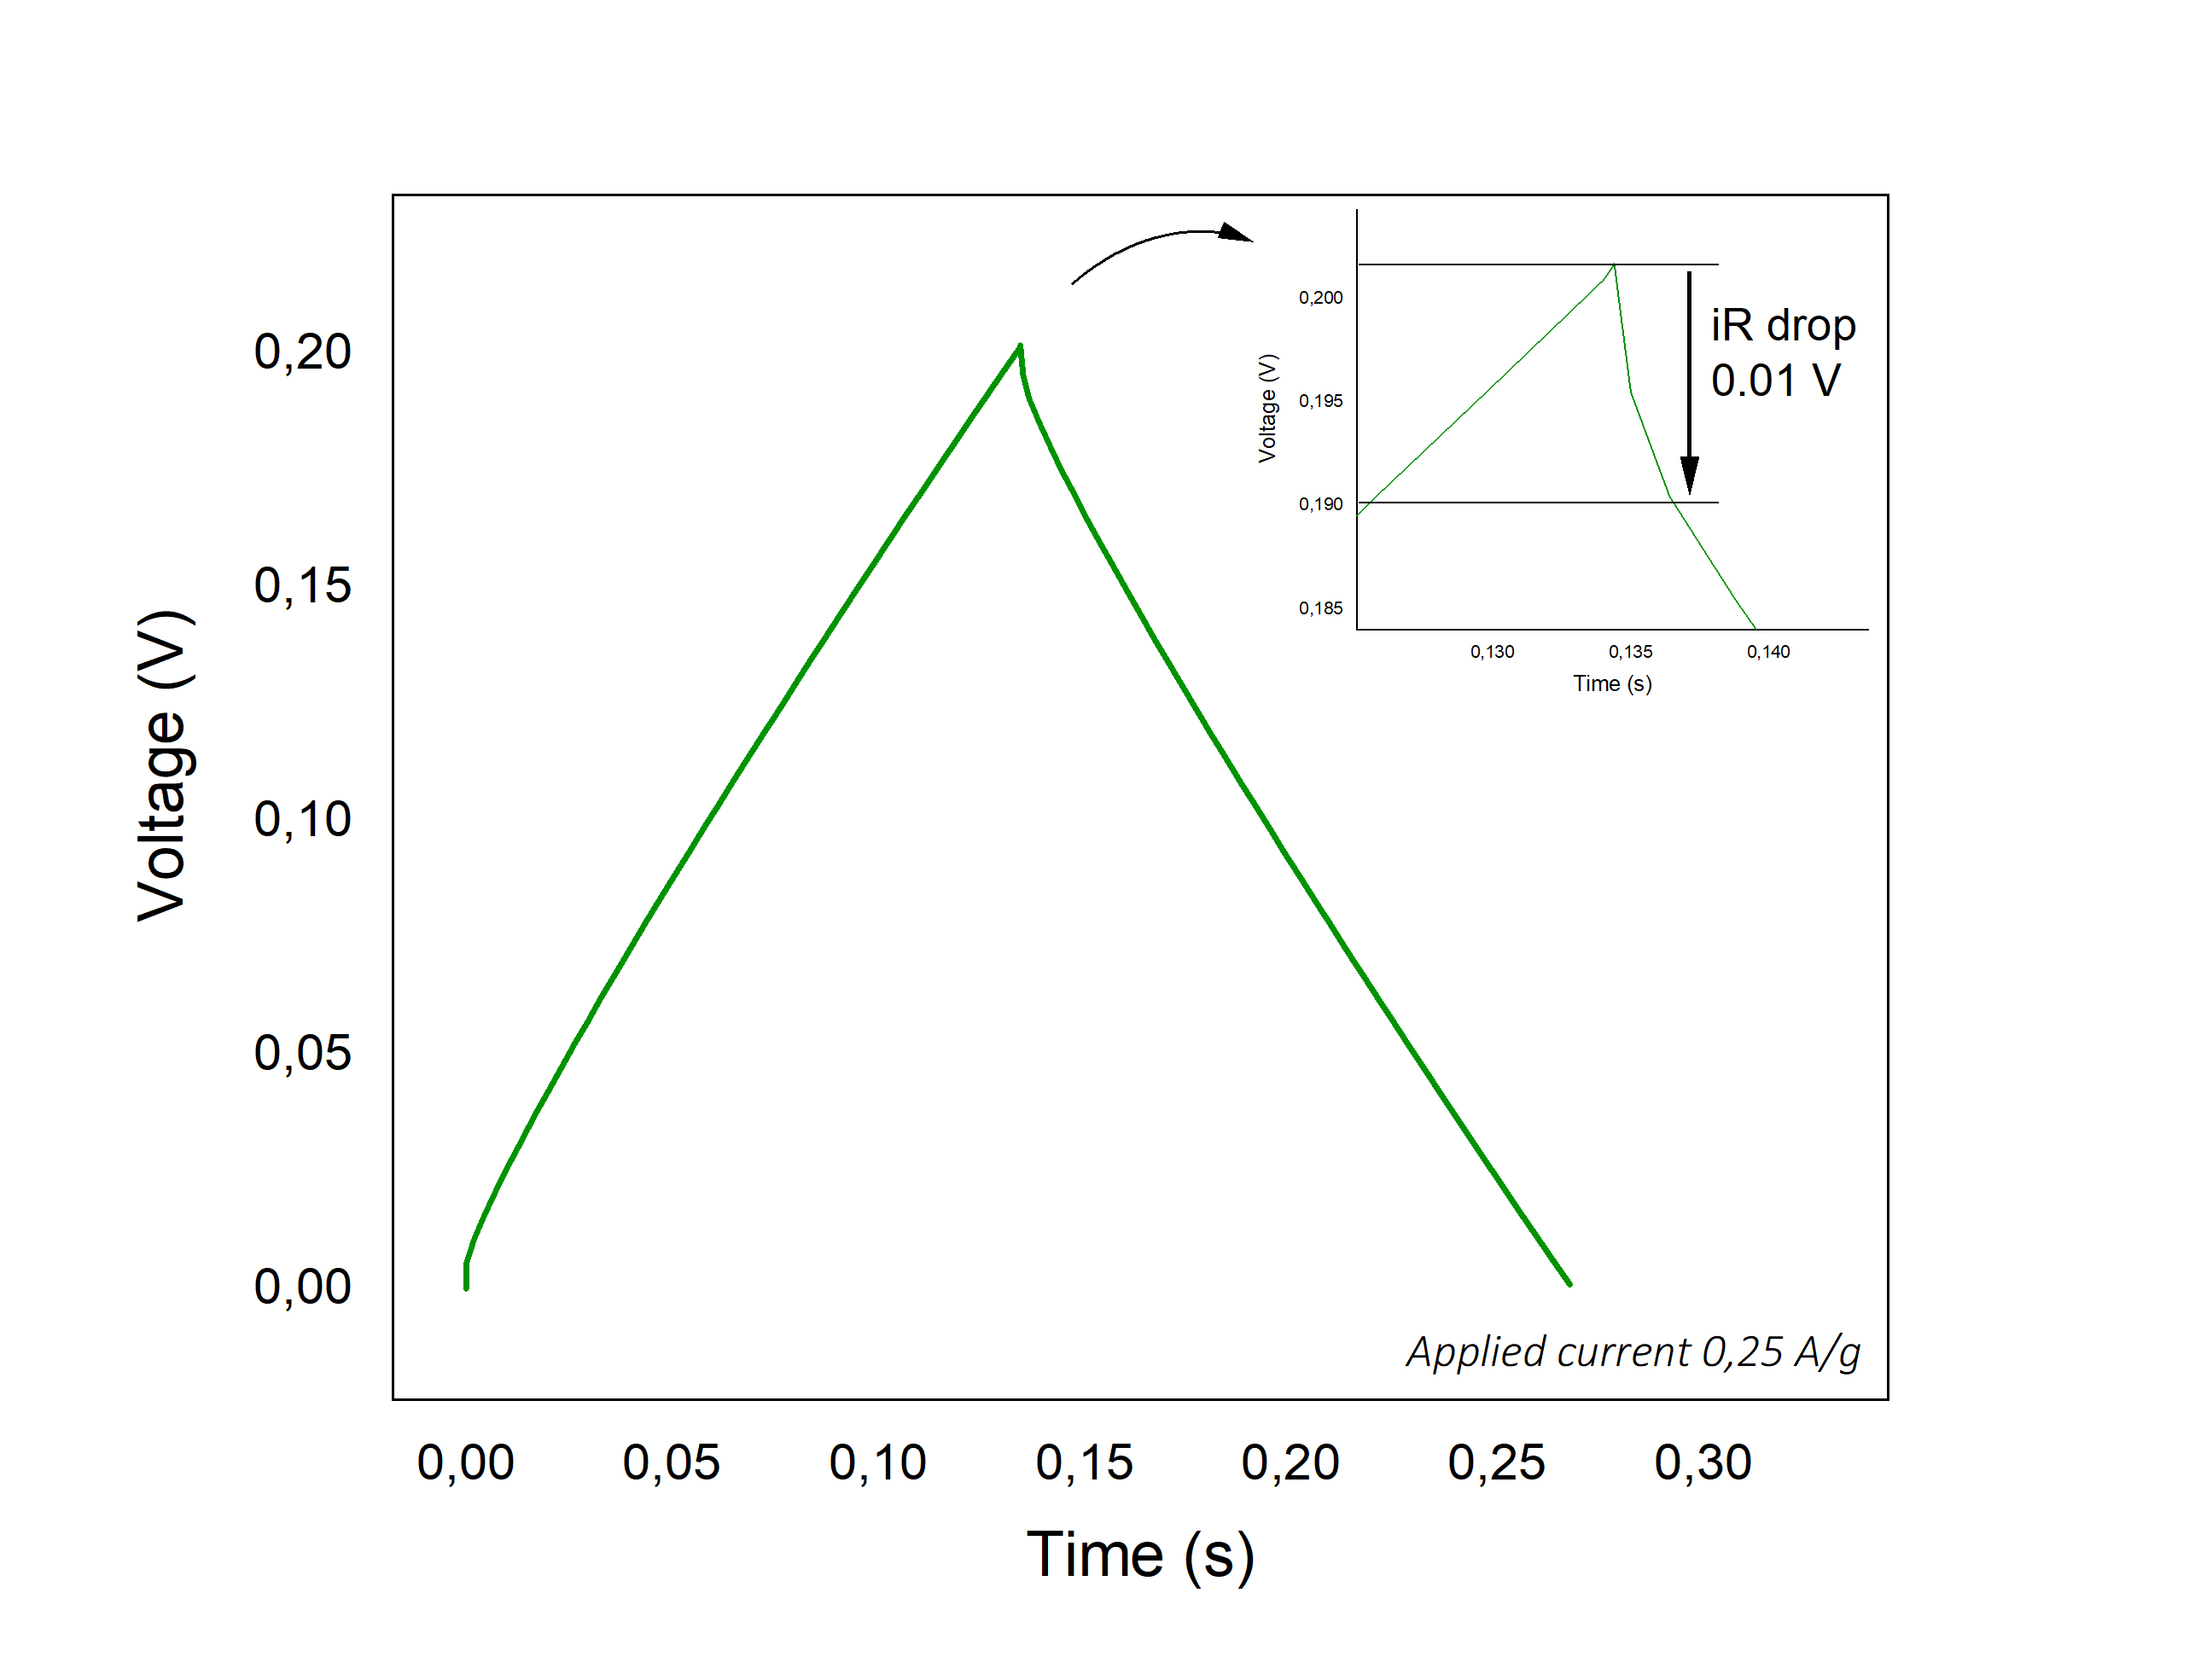
\includegraphics[width=1\textwidth]{Figures/Results/Electrochemistry/LIGF-PI-NaNO3-Swagelok/Cell2/iR-Drop-Low-Current.jpg} 
\captionsetup{width=0.9\linewidth}
\caption{LIGF-Kapton Electrodes, Cell 2 at 100\:mA/s}
\label{fig:LIGF-PI-cell2-iRlow}
\end{subfigure}
\begin{subfigure}{0.49\textwidth}
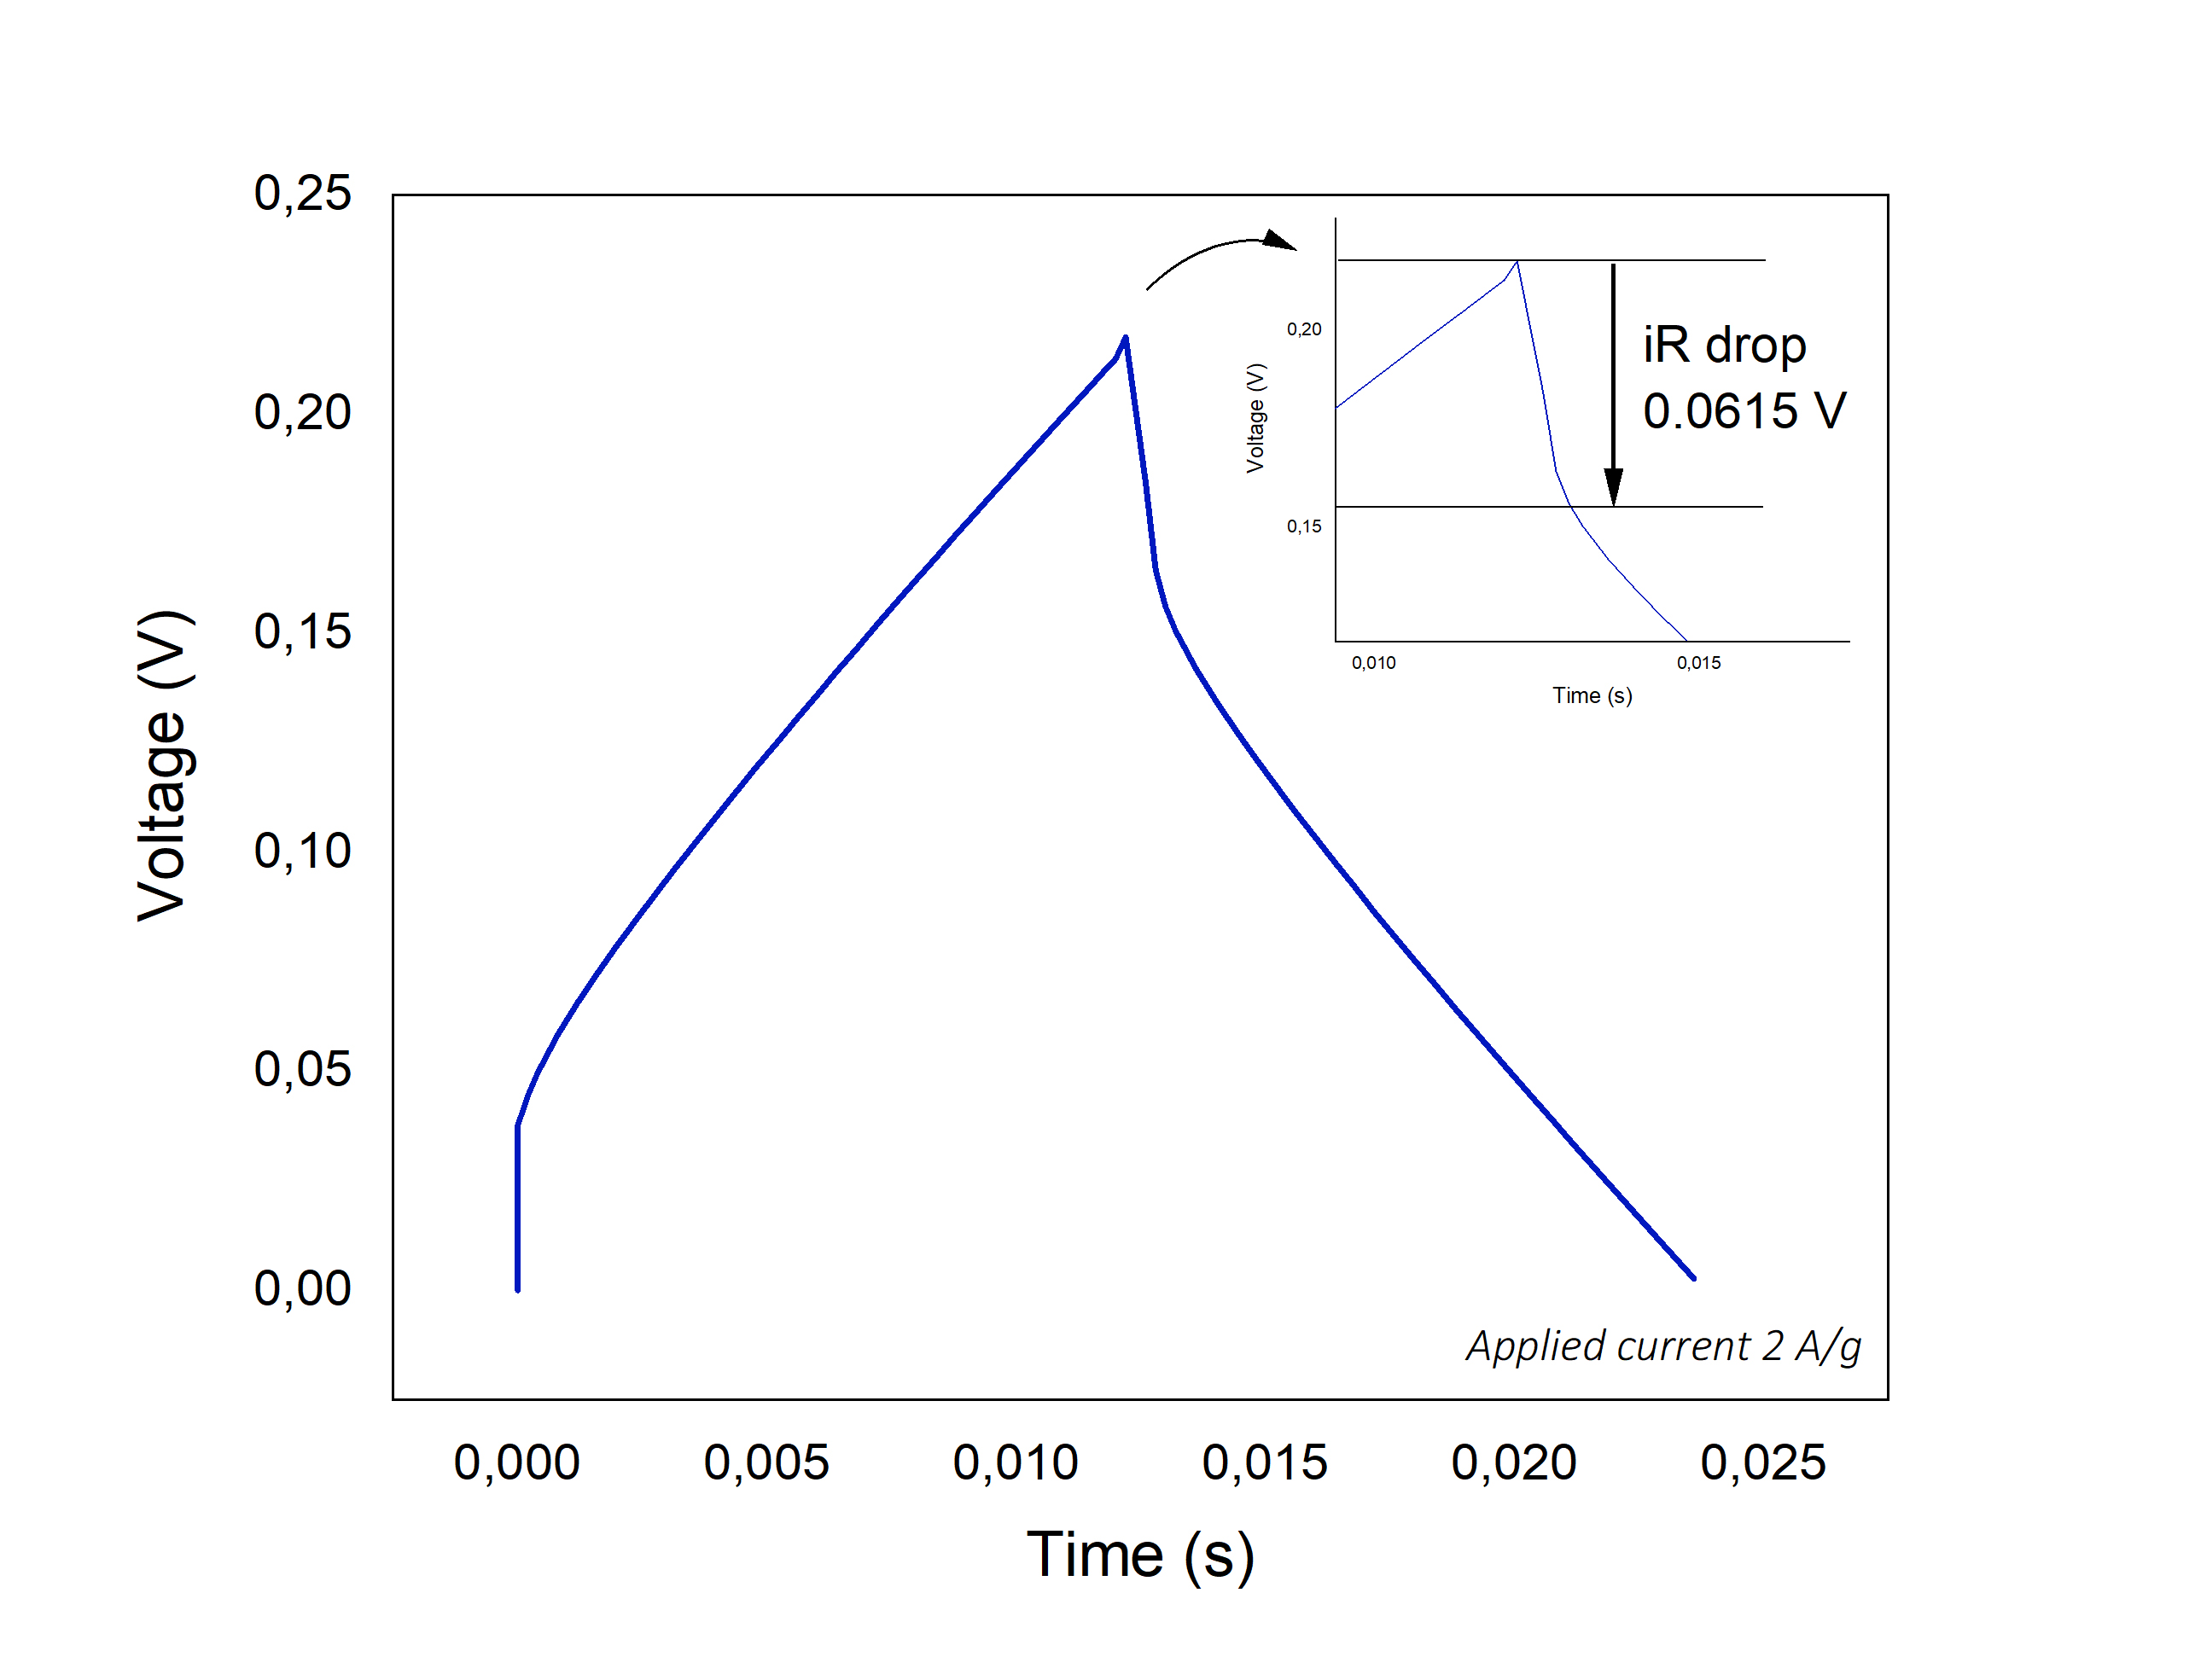
\includegraphics[width=1\textwidth]{Figures/Results/Electrochemistry/LIGF-PI-NaNO3-Swagelok/Cell2/iR-Drop-High-Current.jpg}
\captionsetup{width=0.9\linewidth}
\caption{LIGF-Kapton Electrodes, Cell 2 at 2000\:mA/s}
\label{fig:LIGF-PI-cell2-iRhigh}
\end{subfigure}
\medskip
\caption{CC diagrams of LIGF-Kapton Swagelok Cell 2 for $V_{max}$=0.2 V at 250\:mA/g and 2000\:mA/g demonstrating the rise of the iR drop with an increase of applied current}
\label{fig:LIGF-PI-cell2-iR}
\end{figure}

Further series of CV experiments at larger voltage sweeps at fixed to 5mV/s scan rate could not show satisfactory behaviour of the Cell 2 as the rectangular shape quickly deteriorated with the rise of $\Delta V$ as shown in Figure . The CC curves in turn have shown very good performance, their triangular shape kept staying the same for all tested $V_{max}$ of 0.2, 0.3, 0.4 and 0.5\:V: 

\begin{figure}[H]
\begin{subfigure}{0.49\textwidth}
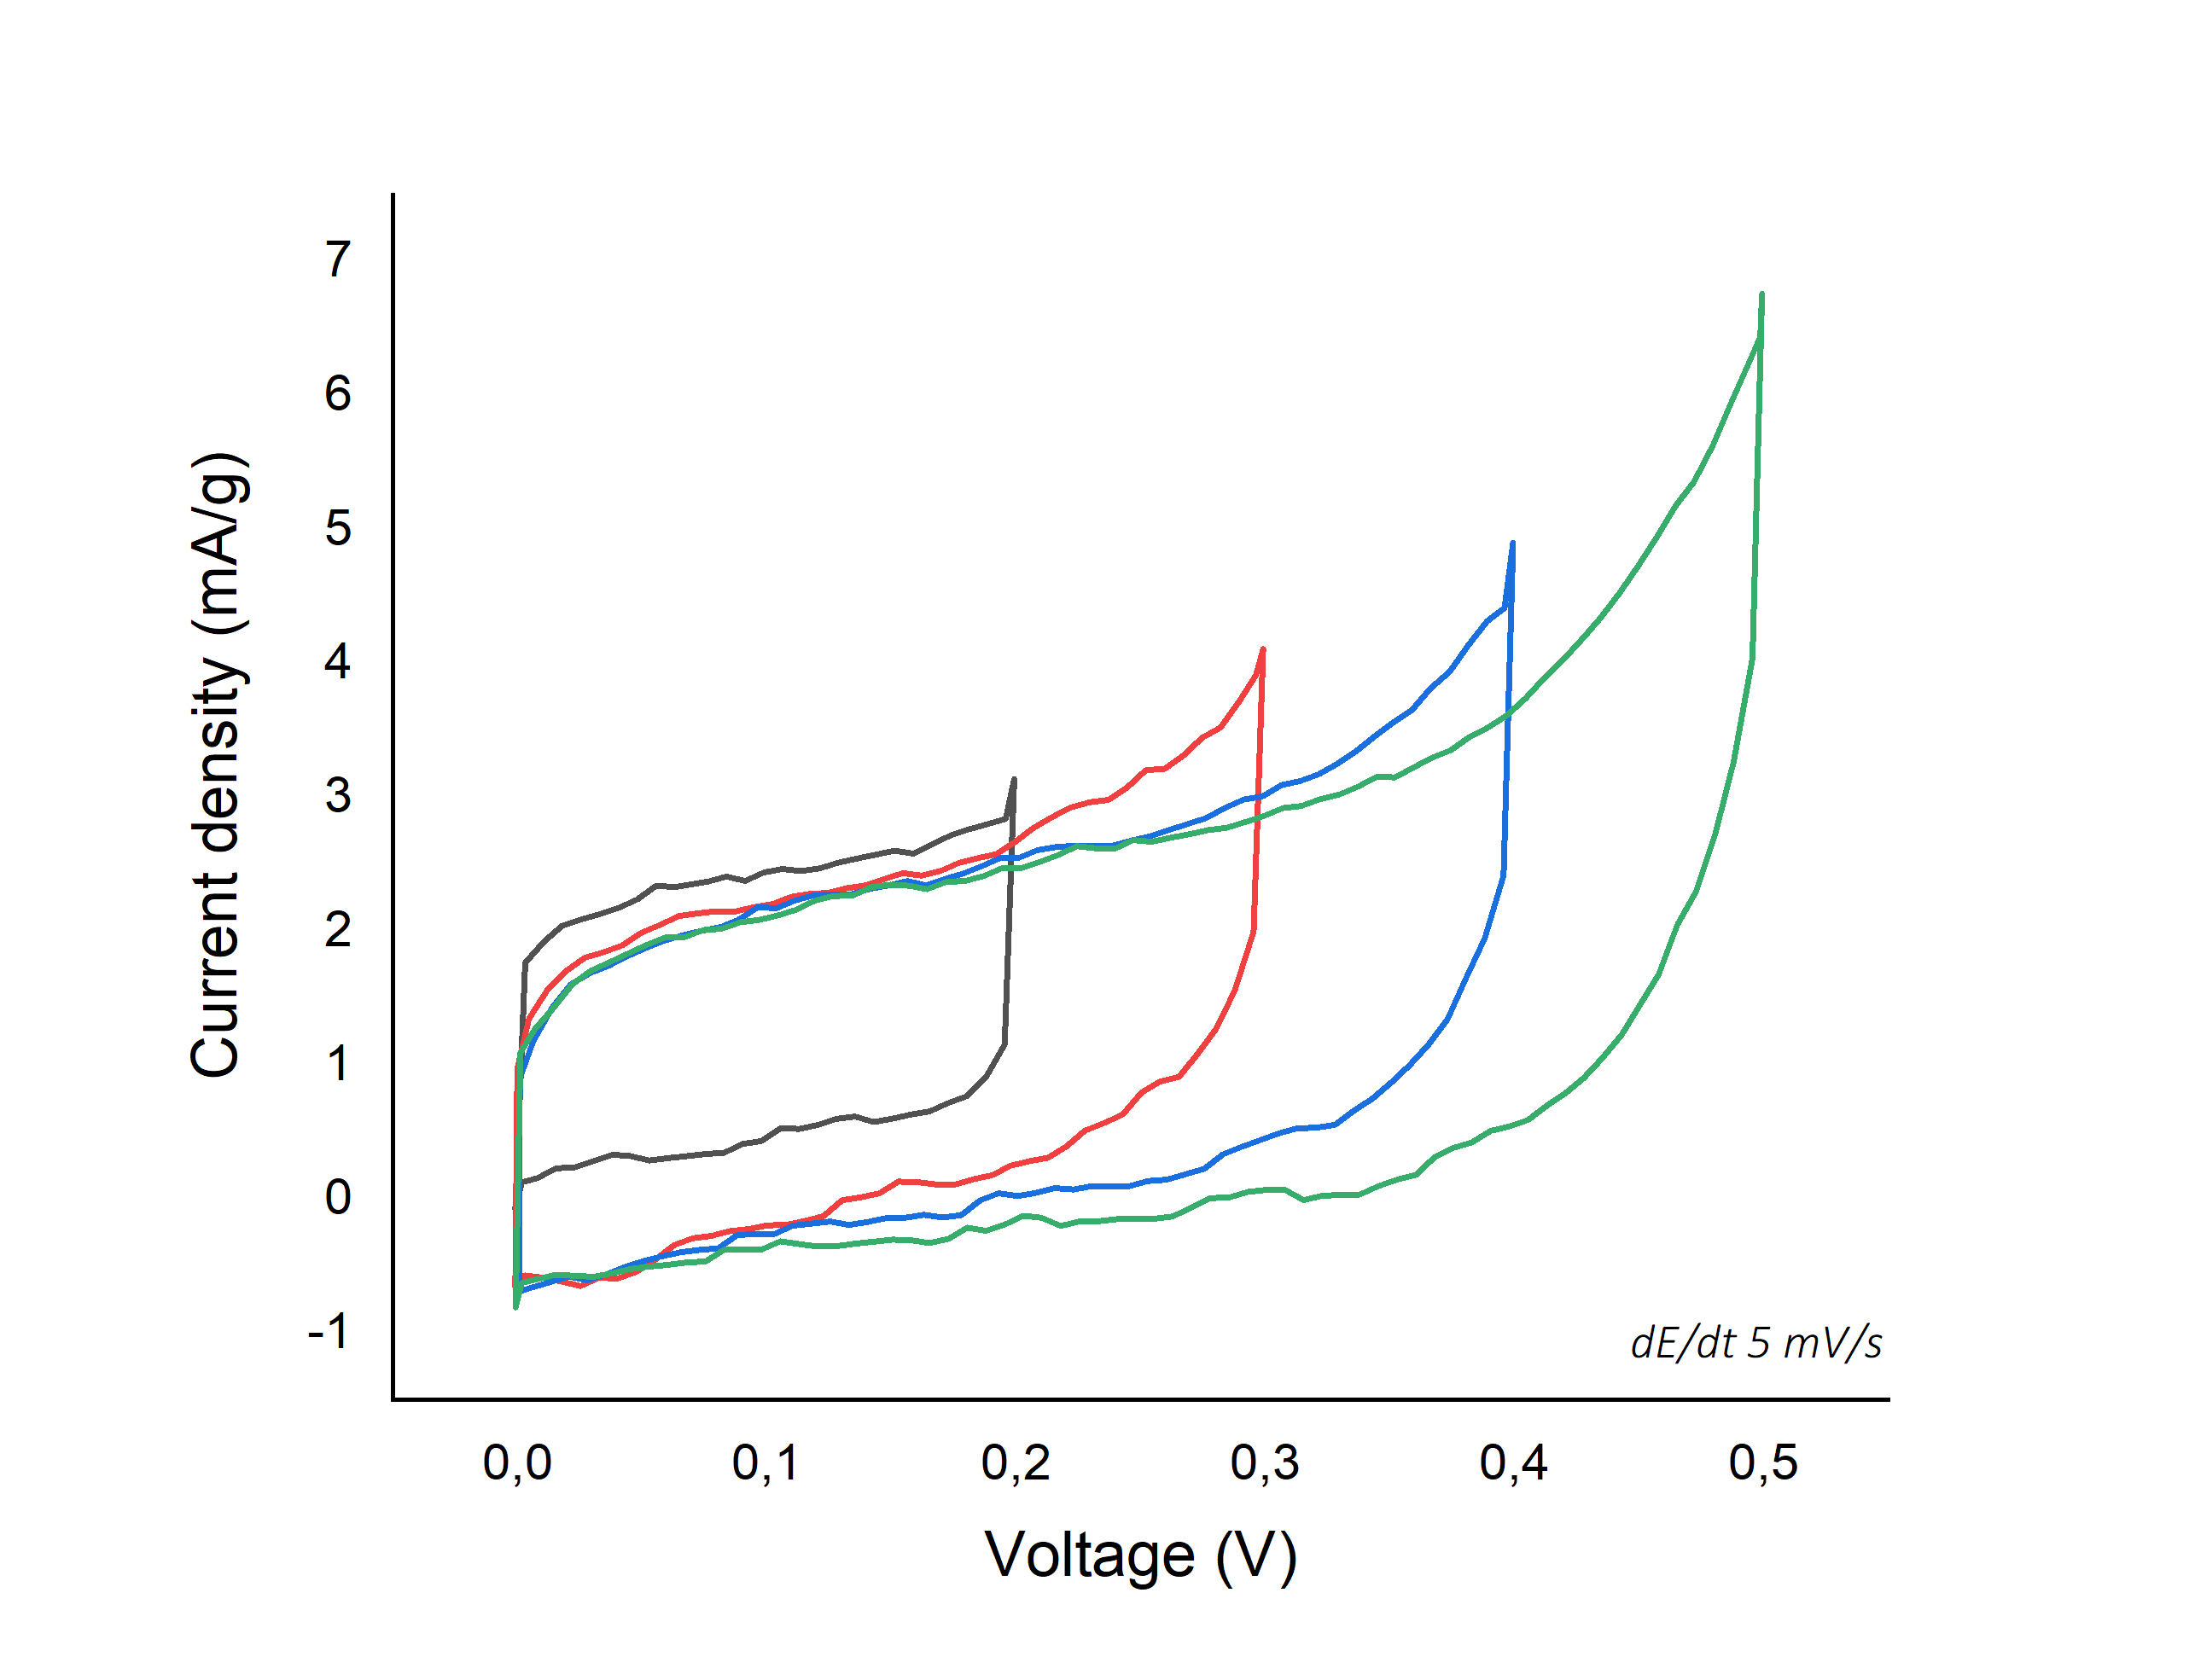
\includegraphics[width=1\textwidth]{Figures/Results/Electrochemistry/LIGF-PI-NaNO3-Swagelok/Cell2/CV-high-5mVs.jpg} 
\captionsetup{width=0.9\linewidth}
\caption{CV diagrams at $\Delta V$ = 0.2$\div$0.5\:V for 5\:mV/s scan rate}
\label{fig:LIGF-PI-cell2-CV06}
\end{subfigure}
\begin{subfigure}{0.49\textwidth}
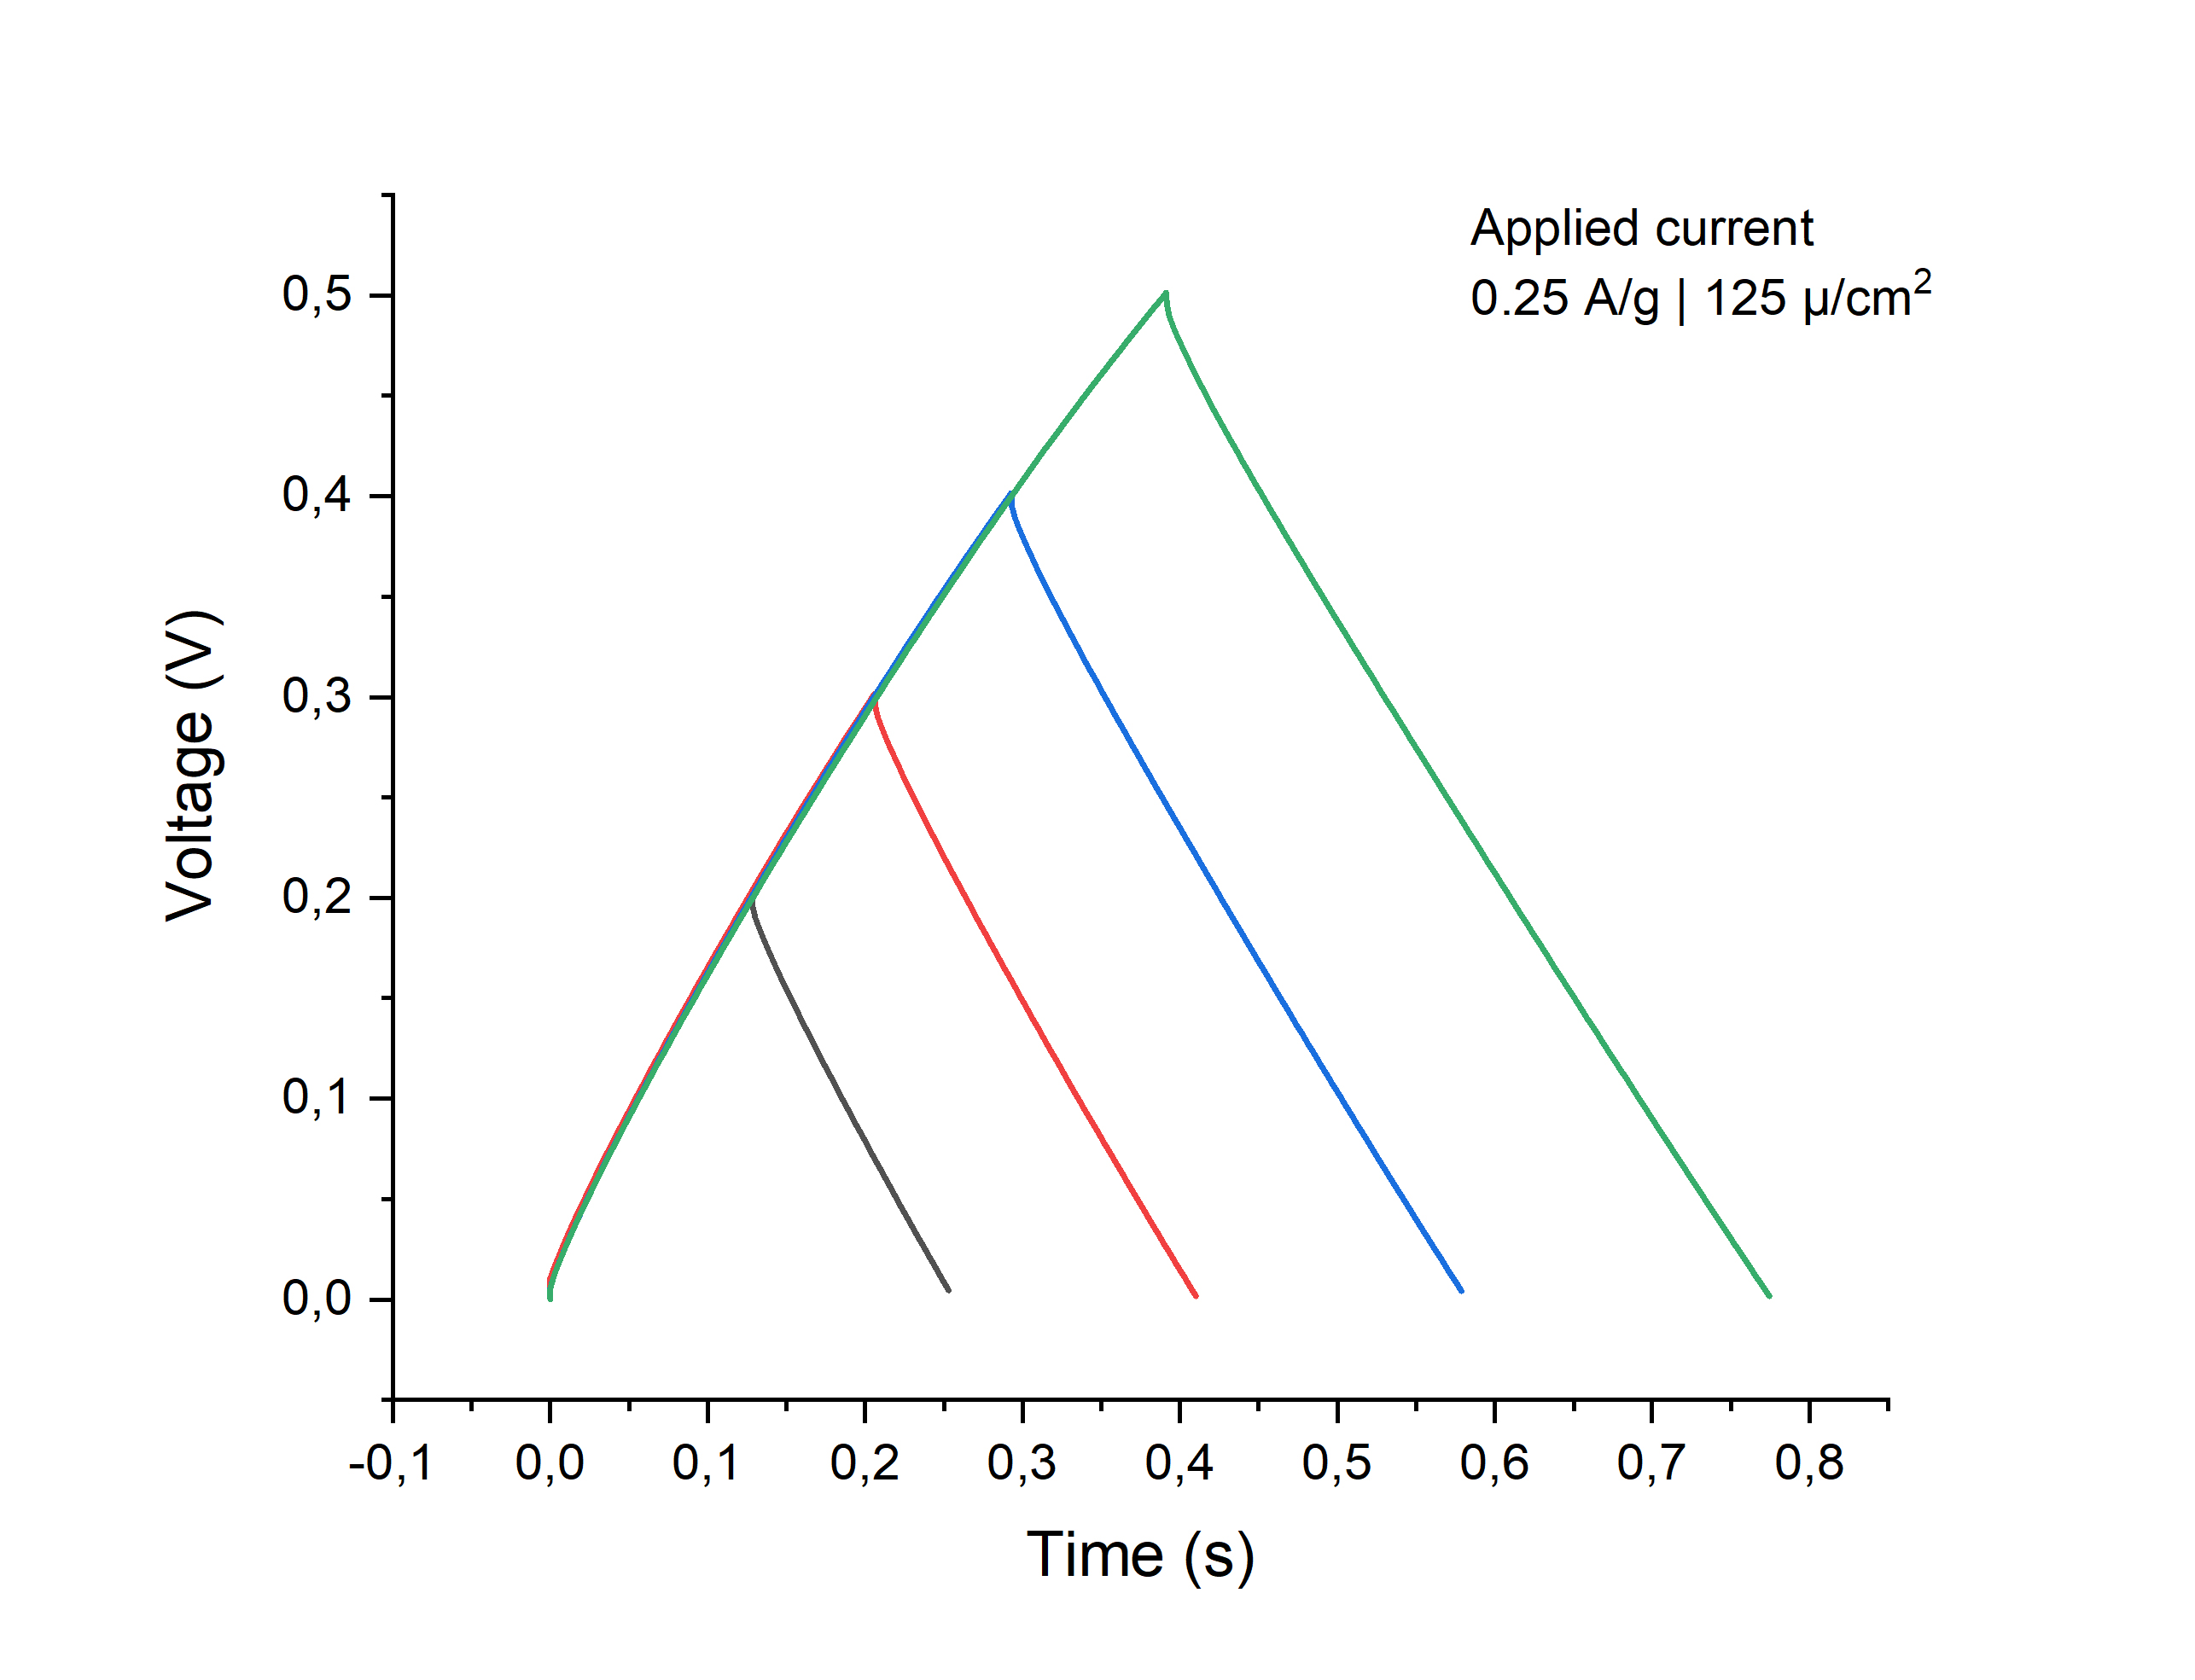
\includegraphics[width=1\textwidth]{Figures/Results/Electrochemistry/LIGF-PI-NaNO3-Swagelok/Cell2/GCPL-high-V.jpg}
\captionsetup{width=0.9\linewidth}
\caption{CC diagrams for $V_{max}$=0.2$\div$0.5\:V at various current densities}
\label{fig:LIGF-PI-cell2-CC06}
\end{subfigure}
\medskip
\caption{LIGF-Kapton Electrodes, Cell 2. CV and GCPL data in the wider voltage range 0 - 0.5 V}
\label{fig:LIGF-PI-cell2-06}
\end{figure}

\textbf{Capacitance Evaluations for LIGF-Kapton Electrodes}

Similarly to LIGP-Kapton Electrodes specific capacitance values were calculated for the data obtained by both cyclic voltammetry and galvanostatic cycling with potential limitation. 

The trend of increasing capacitance with increasing maximum charge potential at constant current,  was preserved for this type of electrode and was similar to the Type 1 ($i.e.$ LIGP-Kapton):

\begin{figure}[H]
\centering
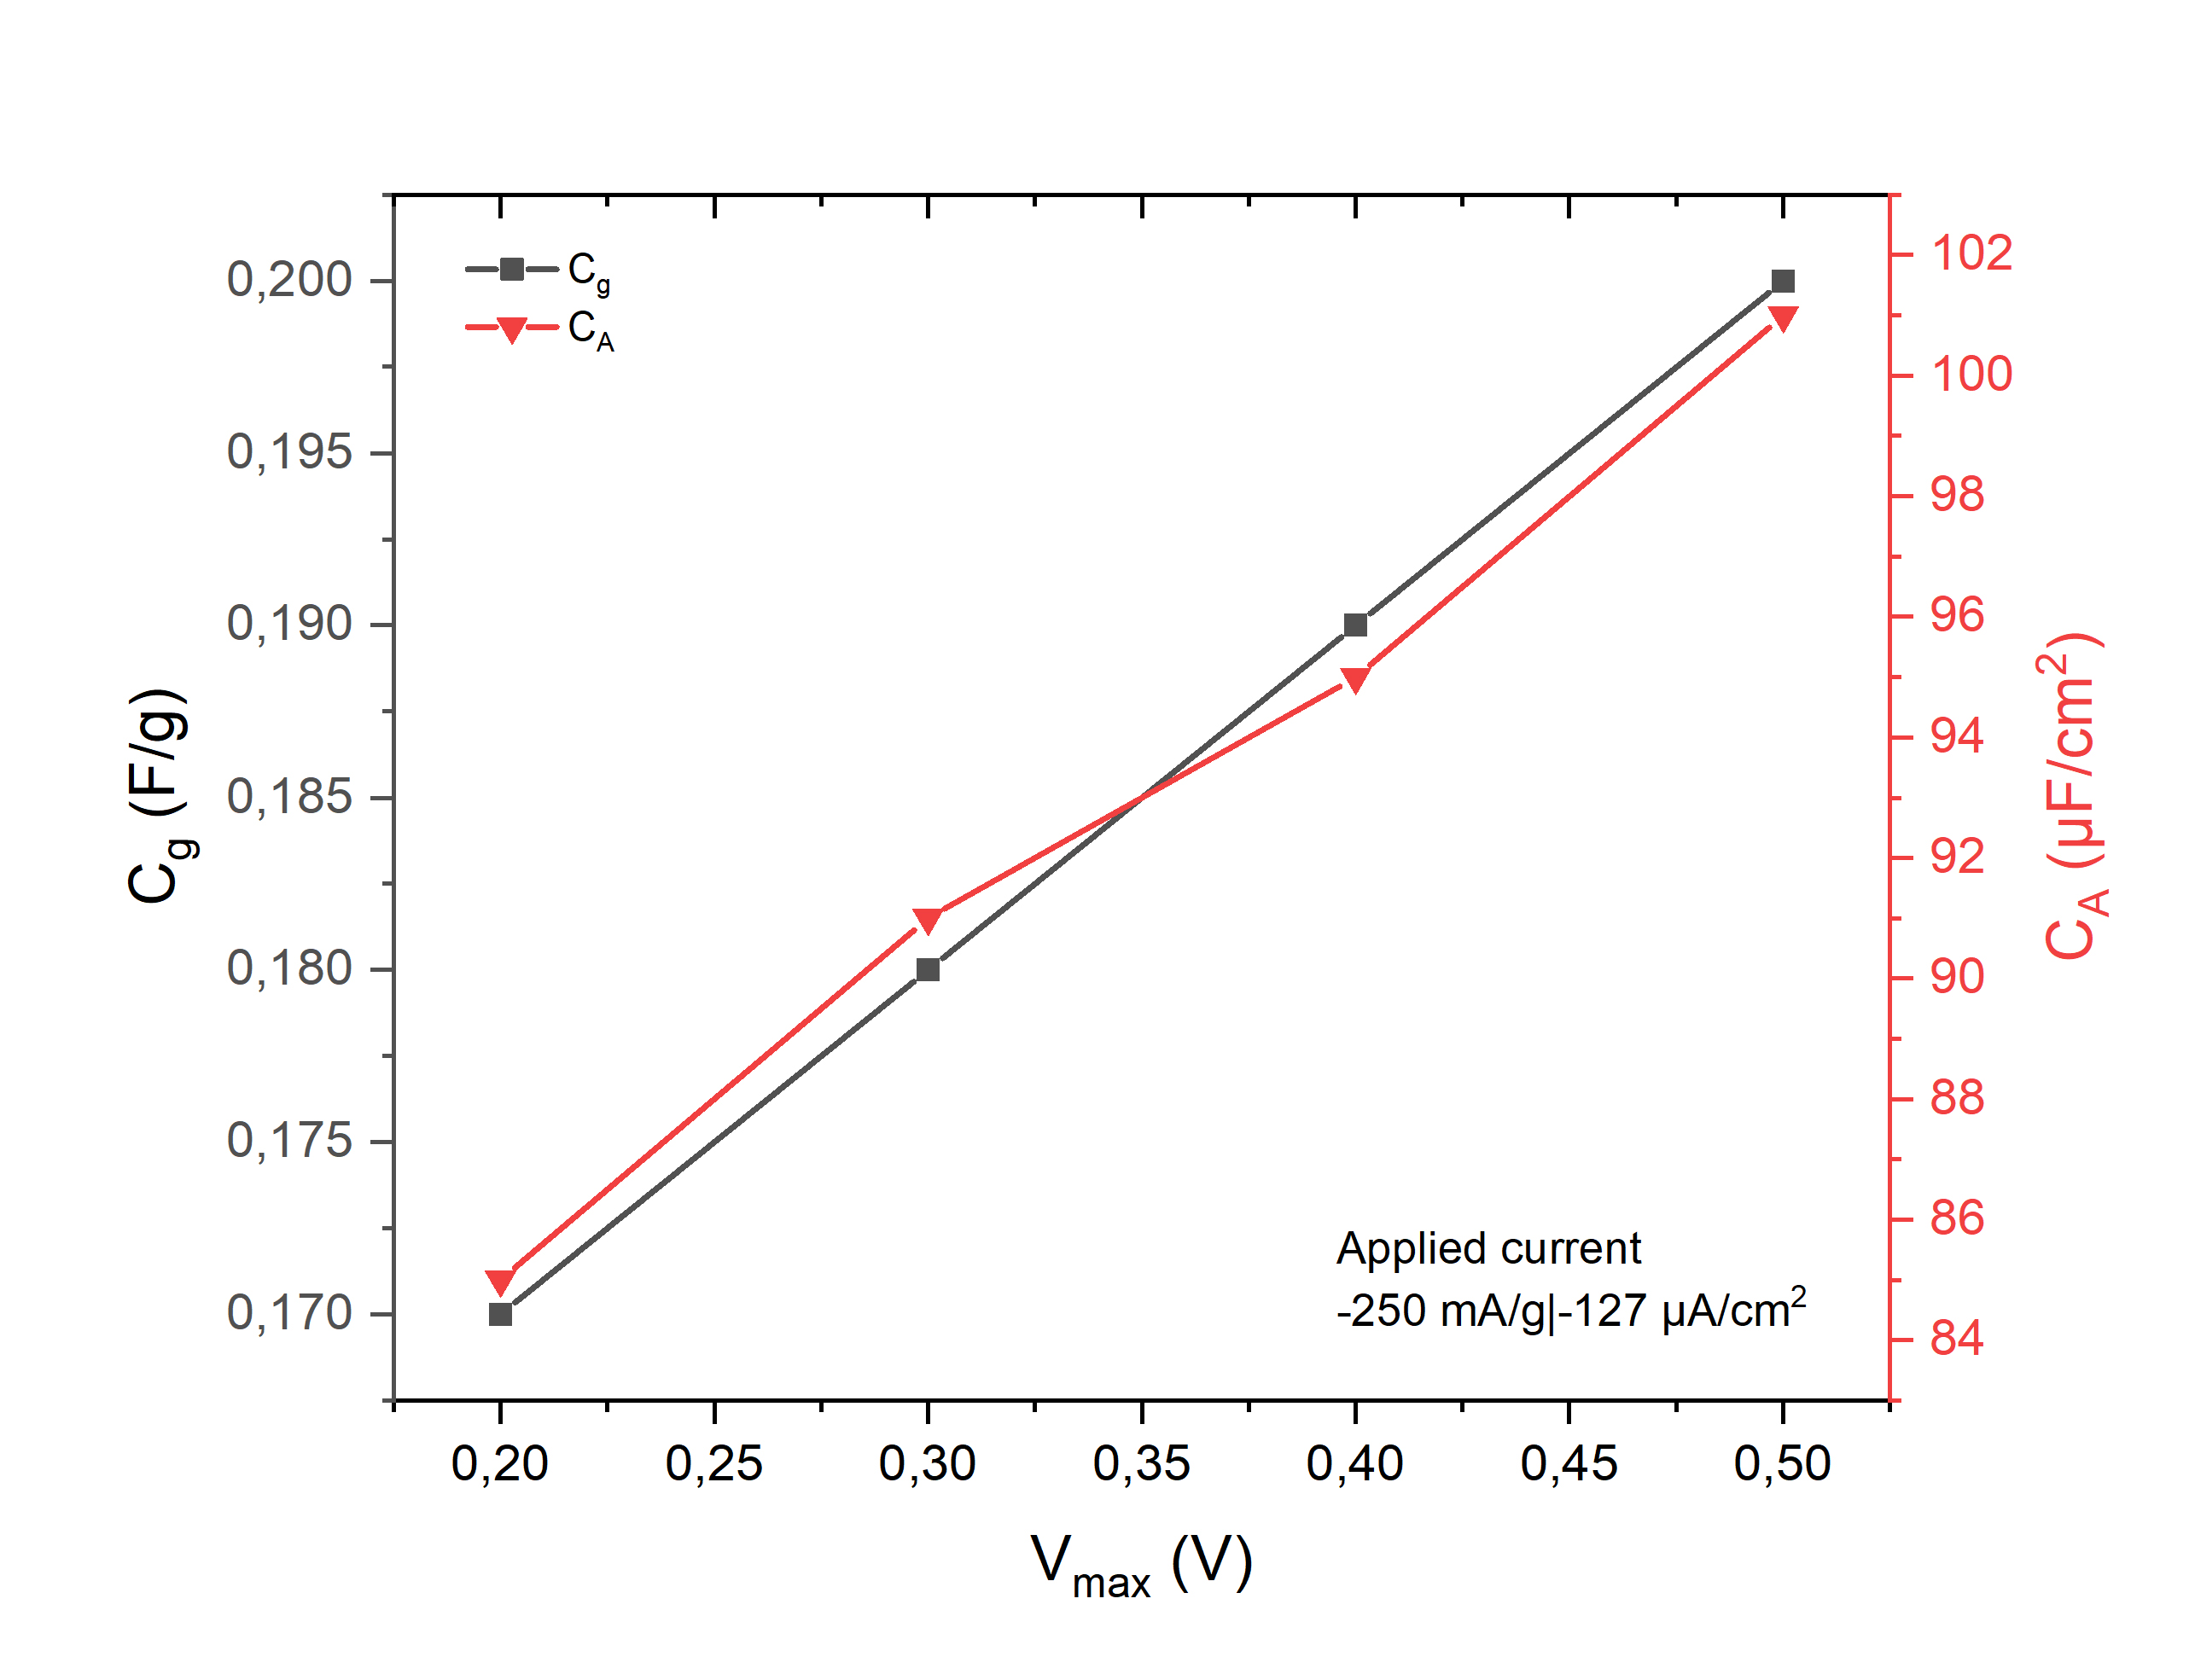
\includegraphics[width=0.6\textwidth]{Figures/Results/Electrochemistry/LIGF-PI-NaNO3-Swagelok/Cell2/Capacitances-Vmax.jpg}
\medskip
\captionsetup{width=0.7\linewidth}
\caption{LIGF-Kapton Electrode - increasing trend in specific capacitance values evaluated from GCPL for increasing charge-discharge current densities at fixed $V_{max}$ = 0.2\:V}
\label{fig:LIGF-PI-capcitance-cc}
\end{figure}

However, and it is interesting to note, that in case of LIGF-Kapton electrodes the values of the capacitance did not show any significant decrease with increasing CV scanning rate. For the galvanostatic experiments with increasing charging-discharging current flowing through the cell for $V_{max}$ set to 0.2\:V a drop of $\approx27\%$ could be observed for the currents increasing from 100 to 2000\:mA/g. Described trends can be seen in Figure \ref{fig:LIGF-PI-capcitance-4}


\begin{figure}[H]
\centering
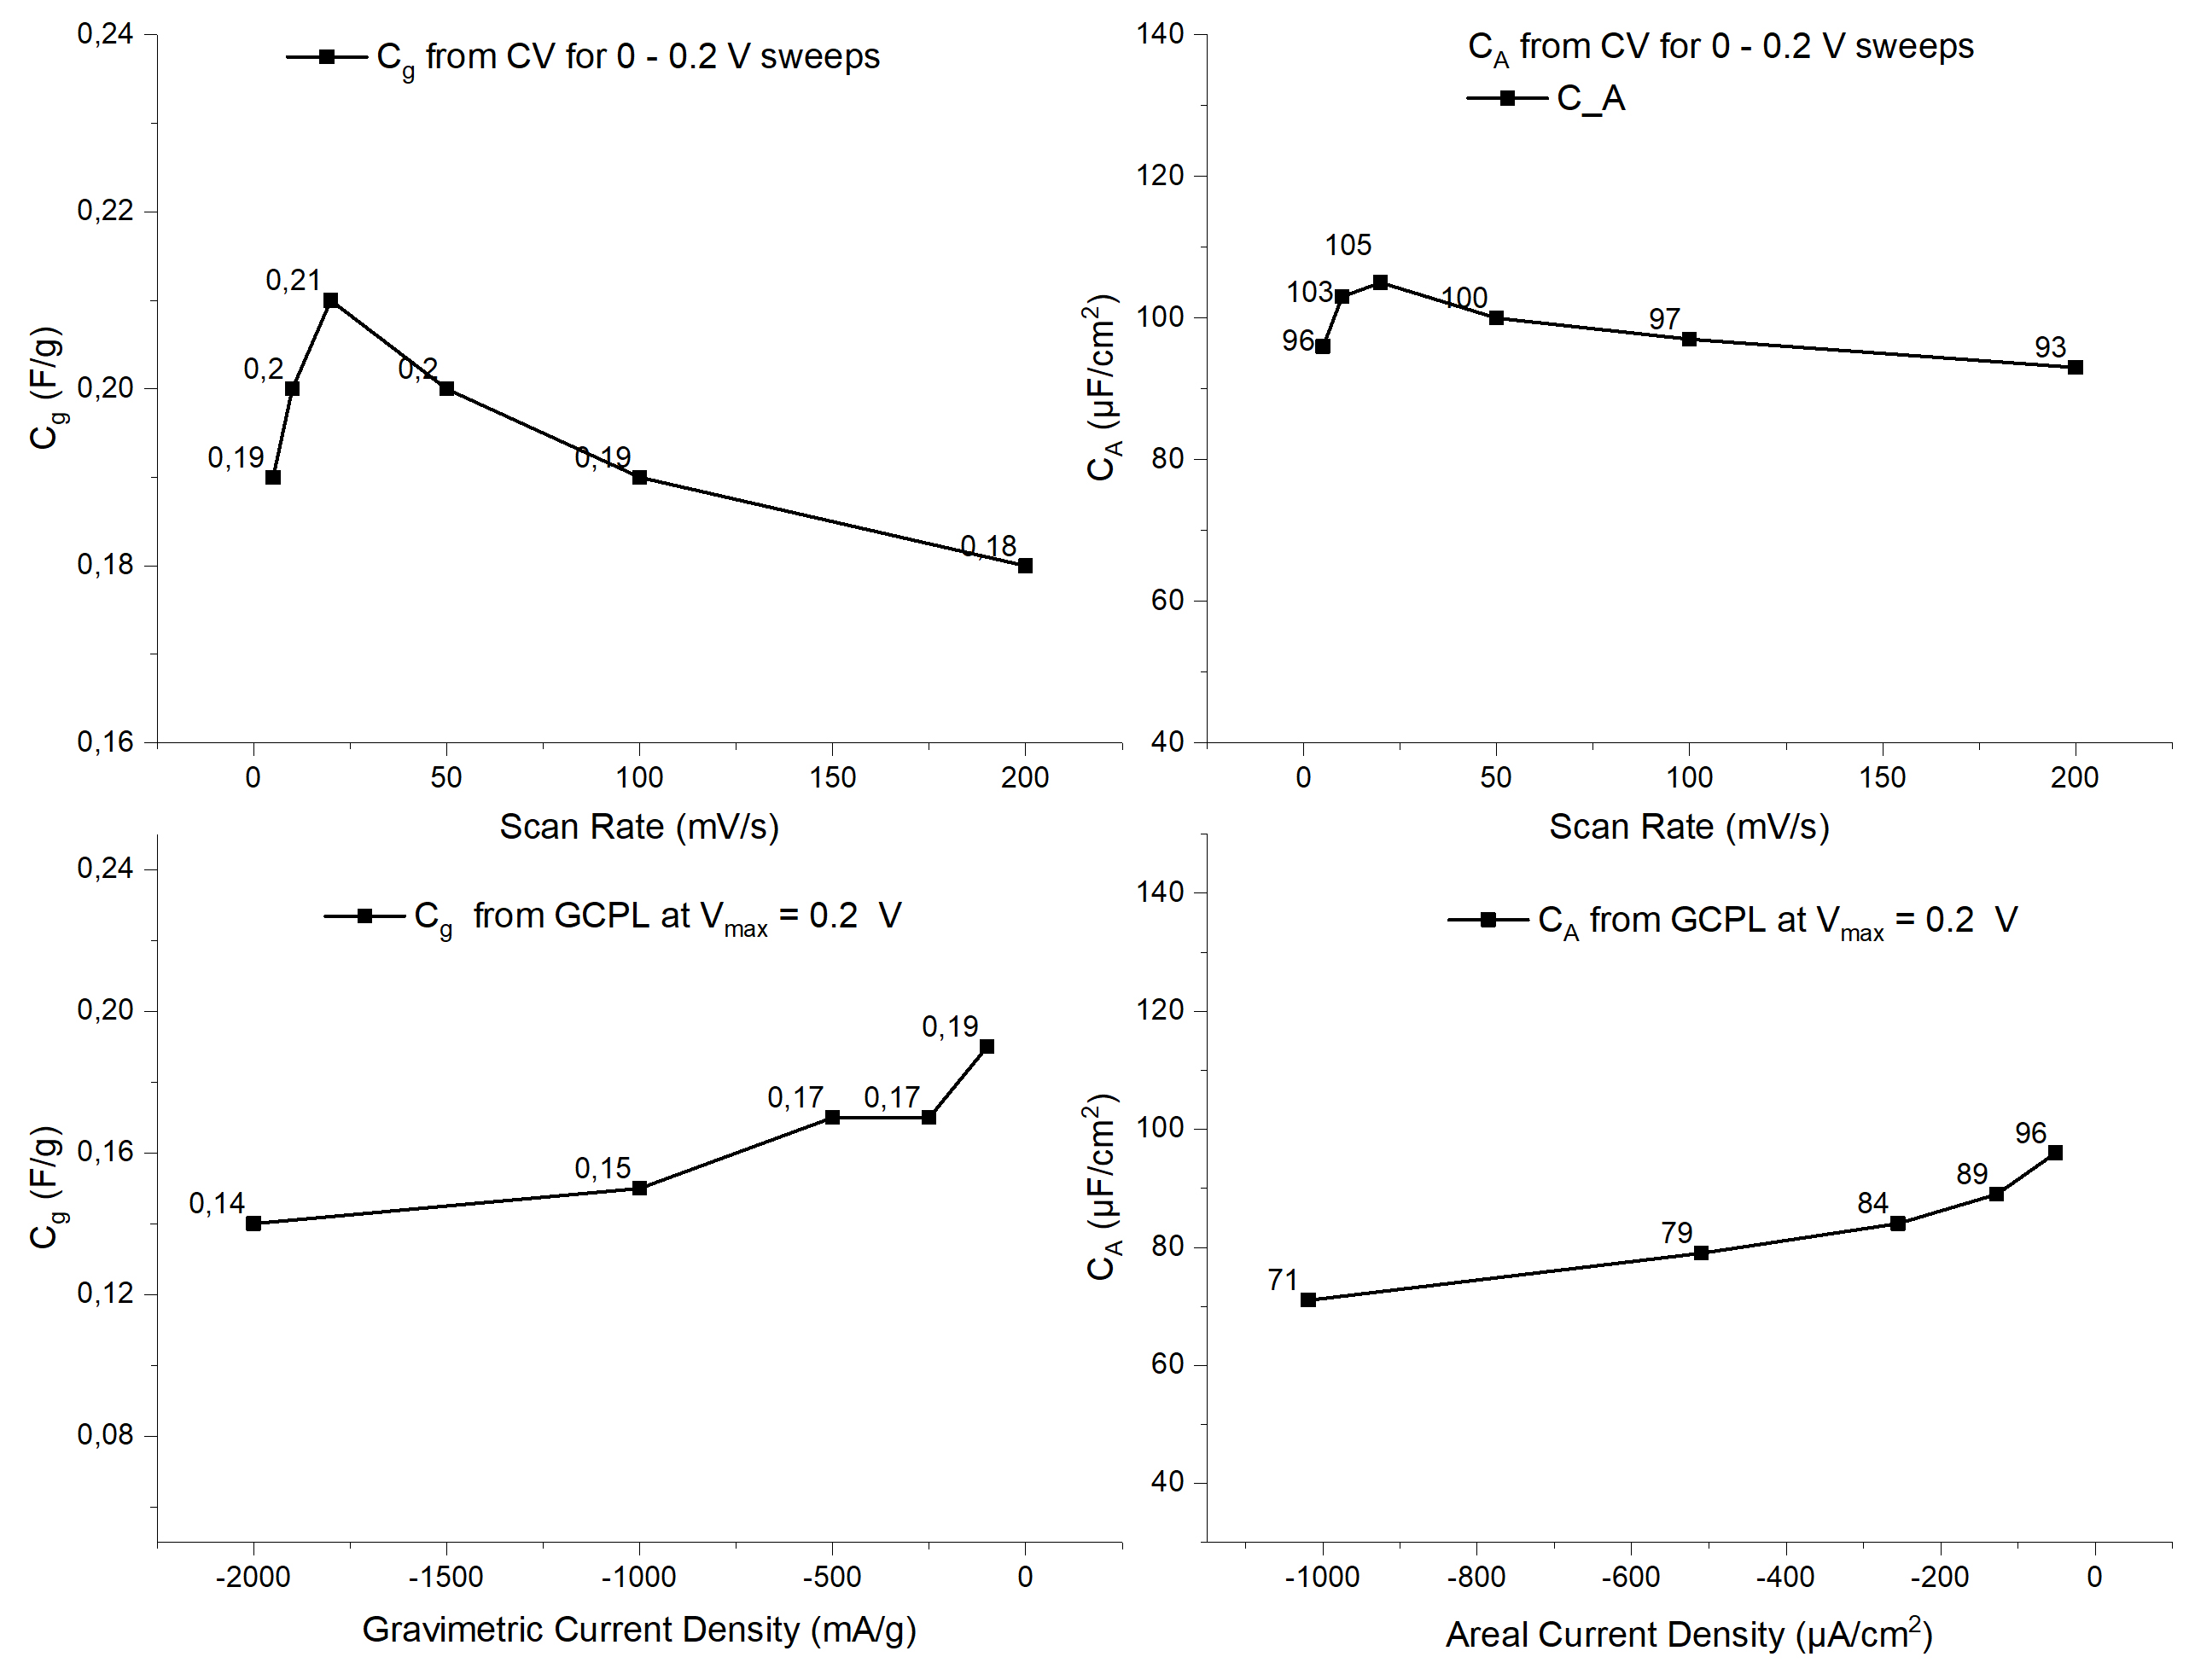
\includegraphics[width=1\textwidth]{Figures/Results/Electrochemistry/LIGF-PI-NaNO3-Swagelok/Cell2/Capacitances-4.jpg}
\medskip
\captionsetup{width=0.7\linewidth}
\caption{LIGF-Kapton Electrode - specific capacitance values evaluated from CV data at voltage window of 0 - 0.2\:V for increasing scan rates $dV/dt$ (top) and from GCPL data for increasing charge-discharge current densities at fixed $V_{max}$ = 0.2\:V (bottom)}
\label{fig:LIGF-PI-capcitance-4}
\end{figure}

XXX Discussion: Does the pore size affect the trends for LIGF-PI? The microporosity and real surface area are poor anyway - that is is why there is no significant diffusion hindrance for the increasing CV scan rates?

.

\textbf{LIGF-PDMS Composite Electrodes in a Swagelok Cell}

The third type of electrode tested was LIGF-PDMS composite (Type 3 in the Table \ref{tab:supercapacitor_electrodes} above). Akin to previous setups two Swagelok cells with 1M NaNO$_3$ as an electrolyte were assembled. However, again the Cell 1 was discarded in the very beginning as it had shown indications of too high inner resistance, probably due to a failure of the VIA contacts,  already during preliminary CV sweeps. 

As for the Cell 2 the tests at lower potentials were performed in the identical manner as before by employing the same protocols for the cyclic voltammetry (increasing scan rates at a fixed voltage window of 0 - 0.2\:V) as well as for the GCPL measurements (increasing charge-discharge current at a fixed $V_{max}=0.2\:V$). As one can see in Figure \ref{fig:LIGF-PDMS-cell2-CC02}, CV curves preserved the rectangular shape, however the galvanostatic curves at all currents were showing obvious distortions from the desirable for supercapacitors triangular shape.  

\begin{figure}[H]
\begin{subfigure}{0.49\textwidth}
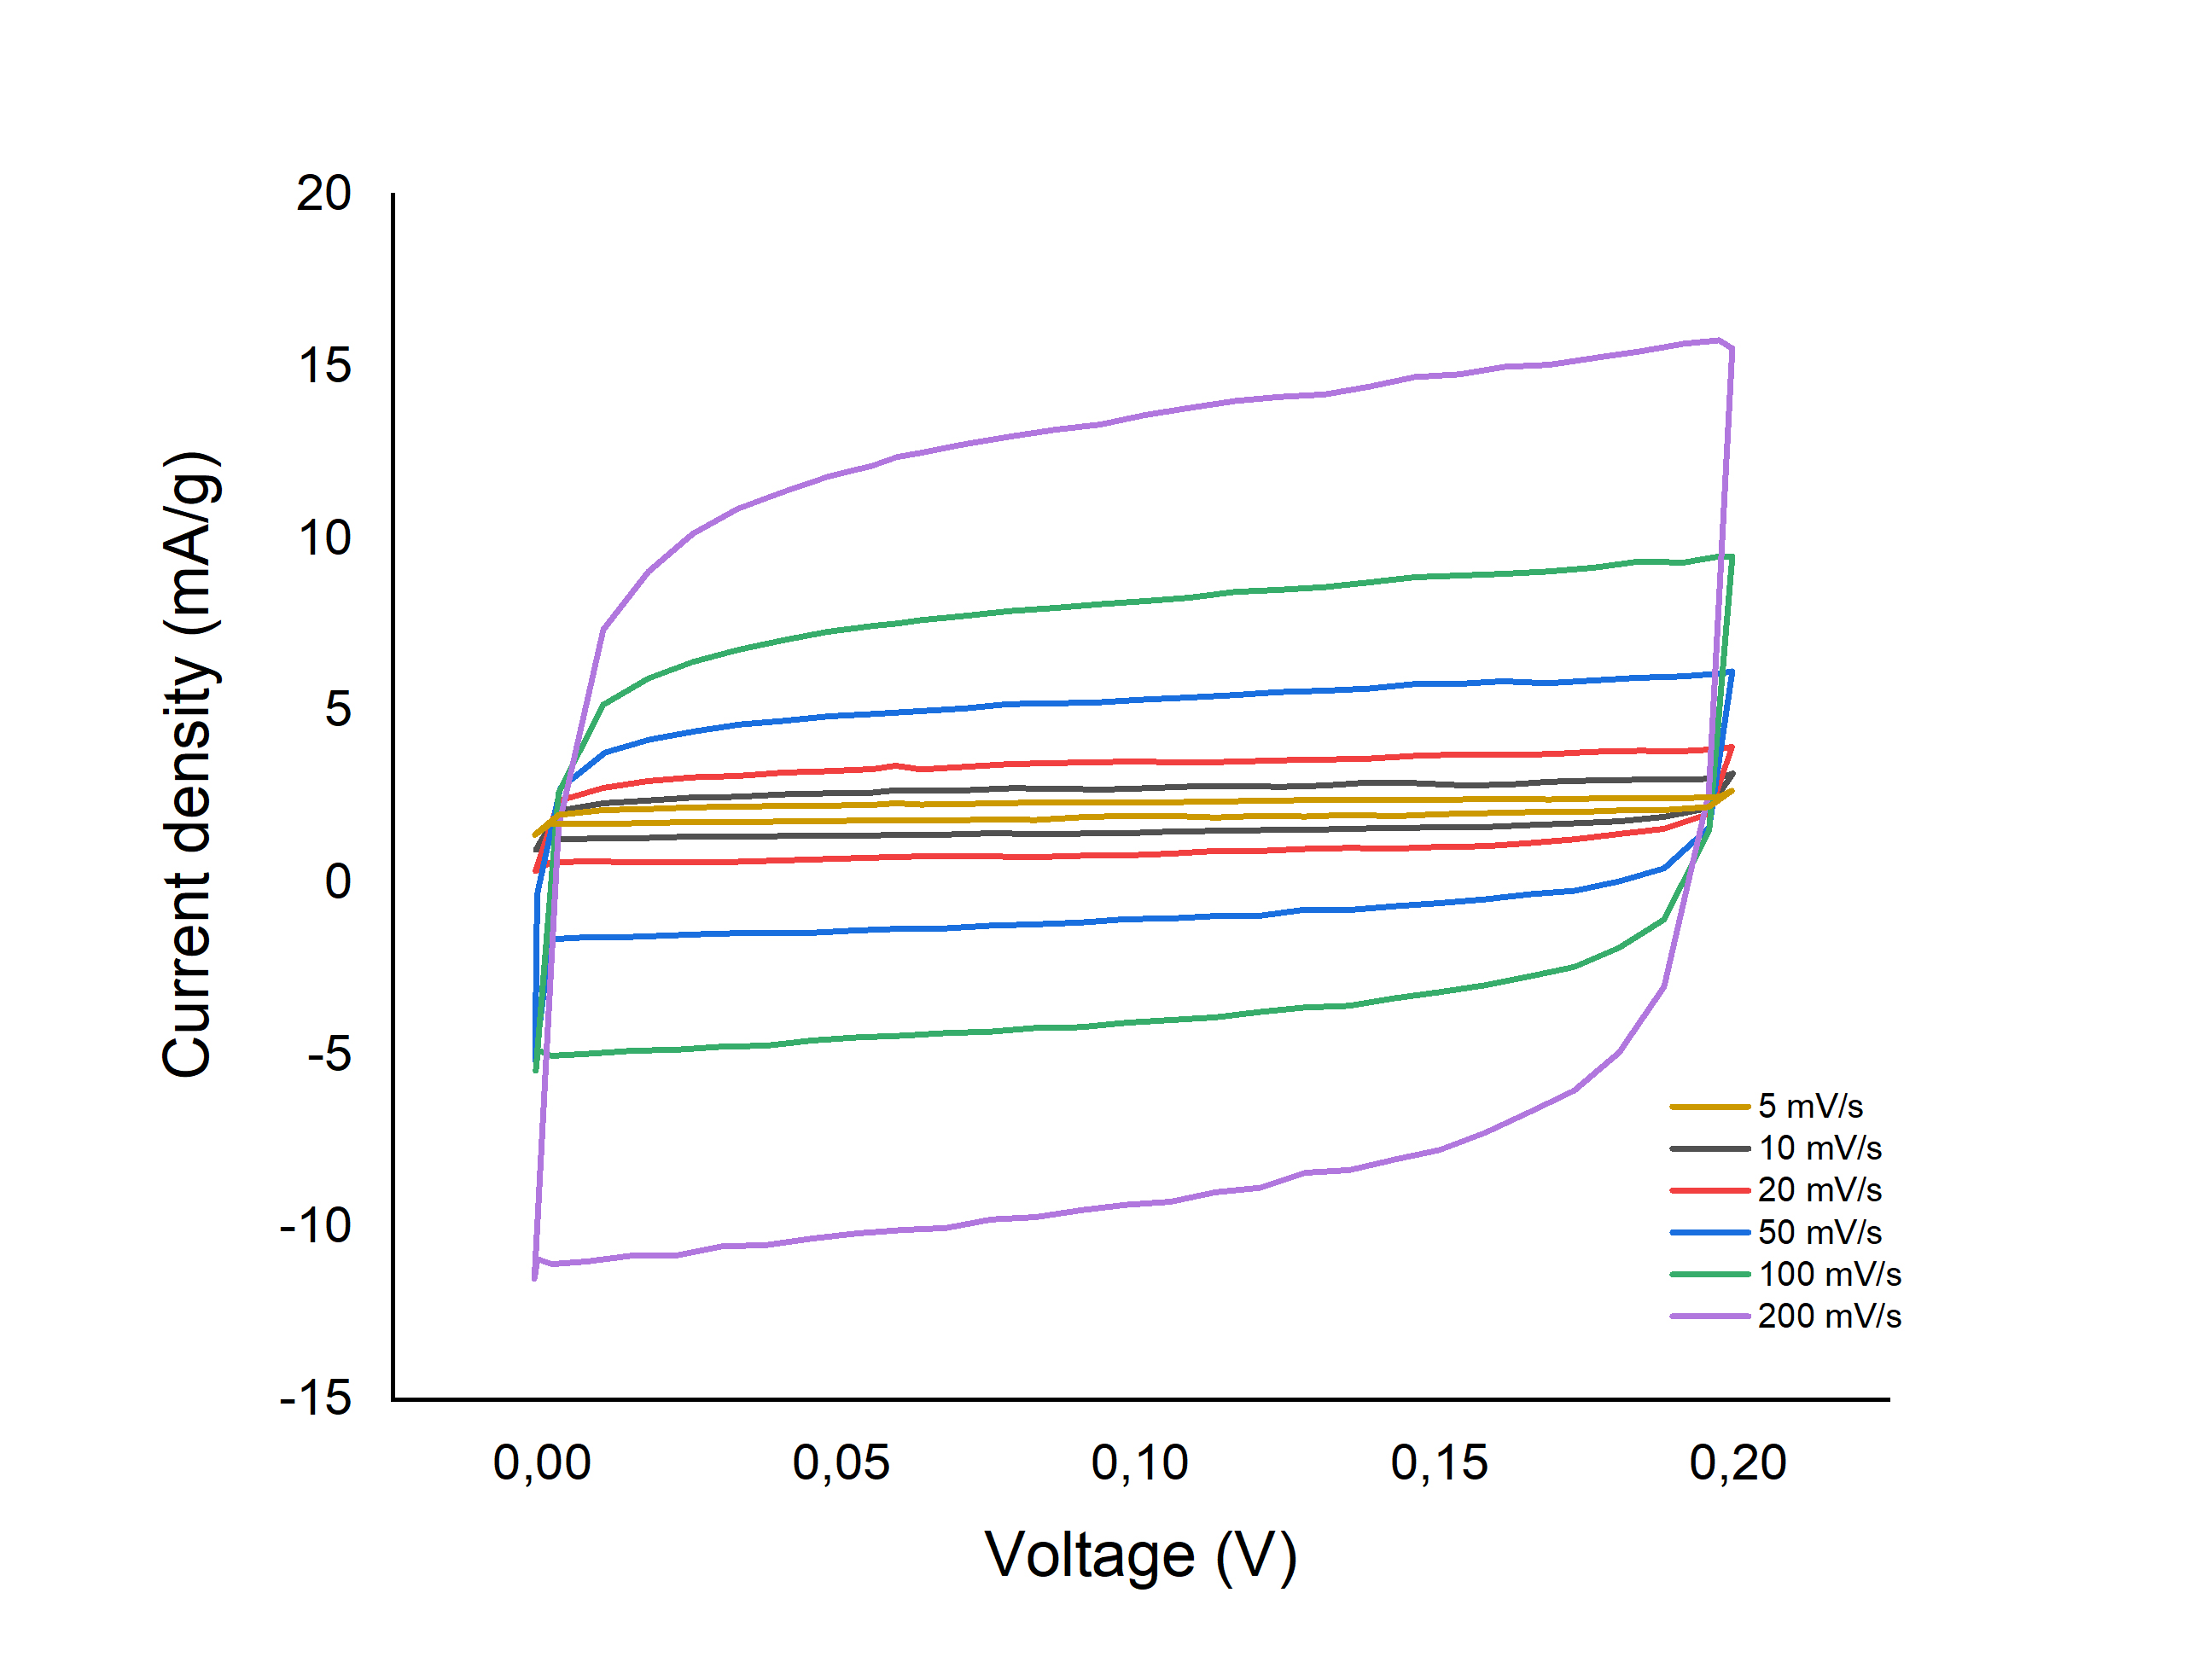
\includegraphics[width=1\textwidth]{Figures/Results/Electrochemistry/LIGF-PDMS-NaNO3-Swagelok/Cell2/CV-V02-Cell2.jpg} 
\captionsetup{width=0.9\linewidth}
\caption{CV diagrams at 0 - 0.2 V potential window at different scan rates}
\label{fig:LIGF-PDMS-cell2-CV02}
\end{subfigure}
\begin{subfigure}{0.49\textwidth}
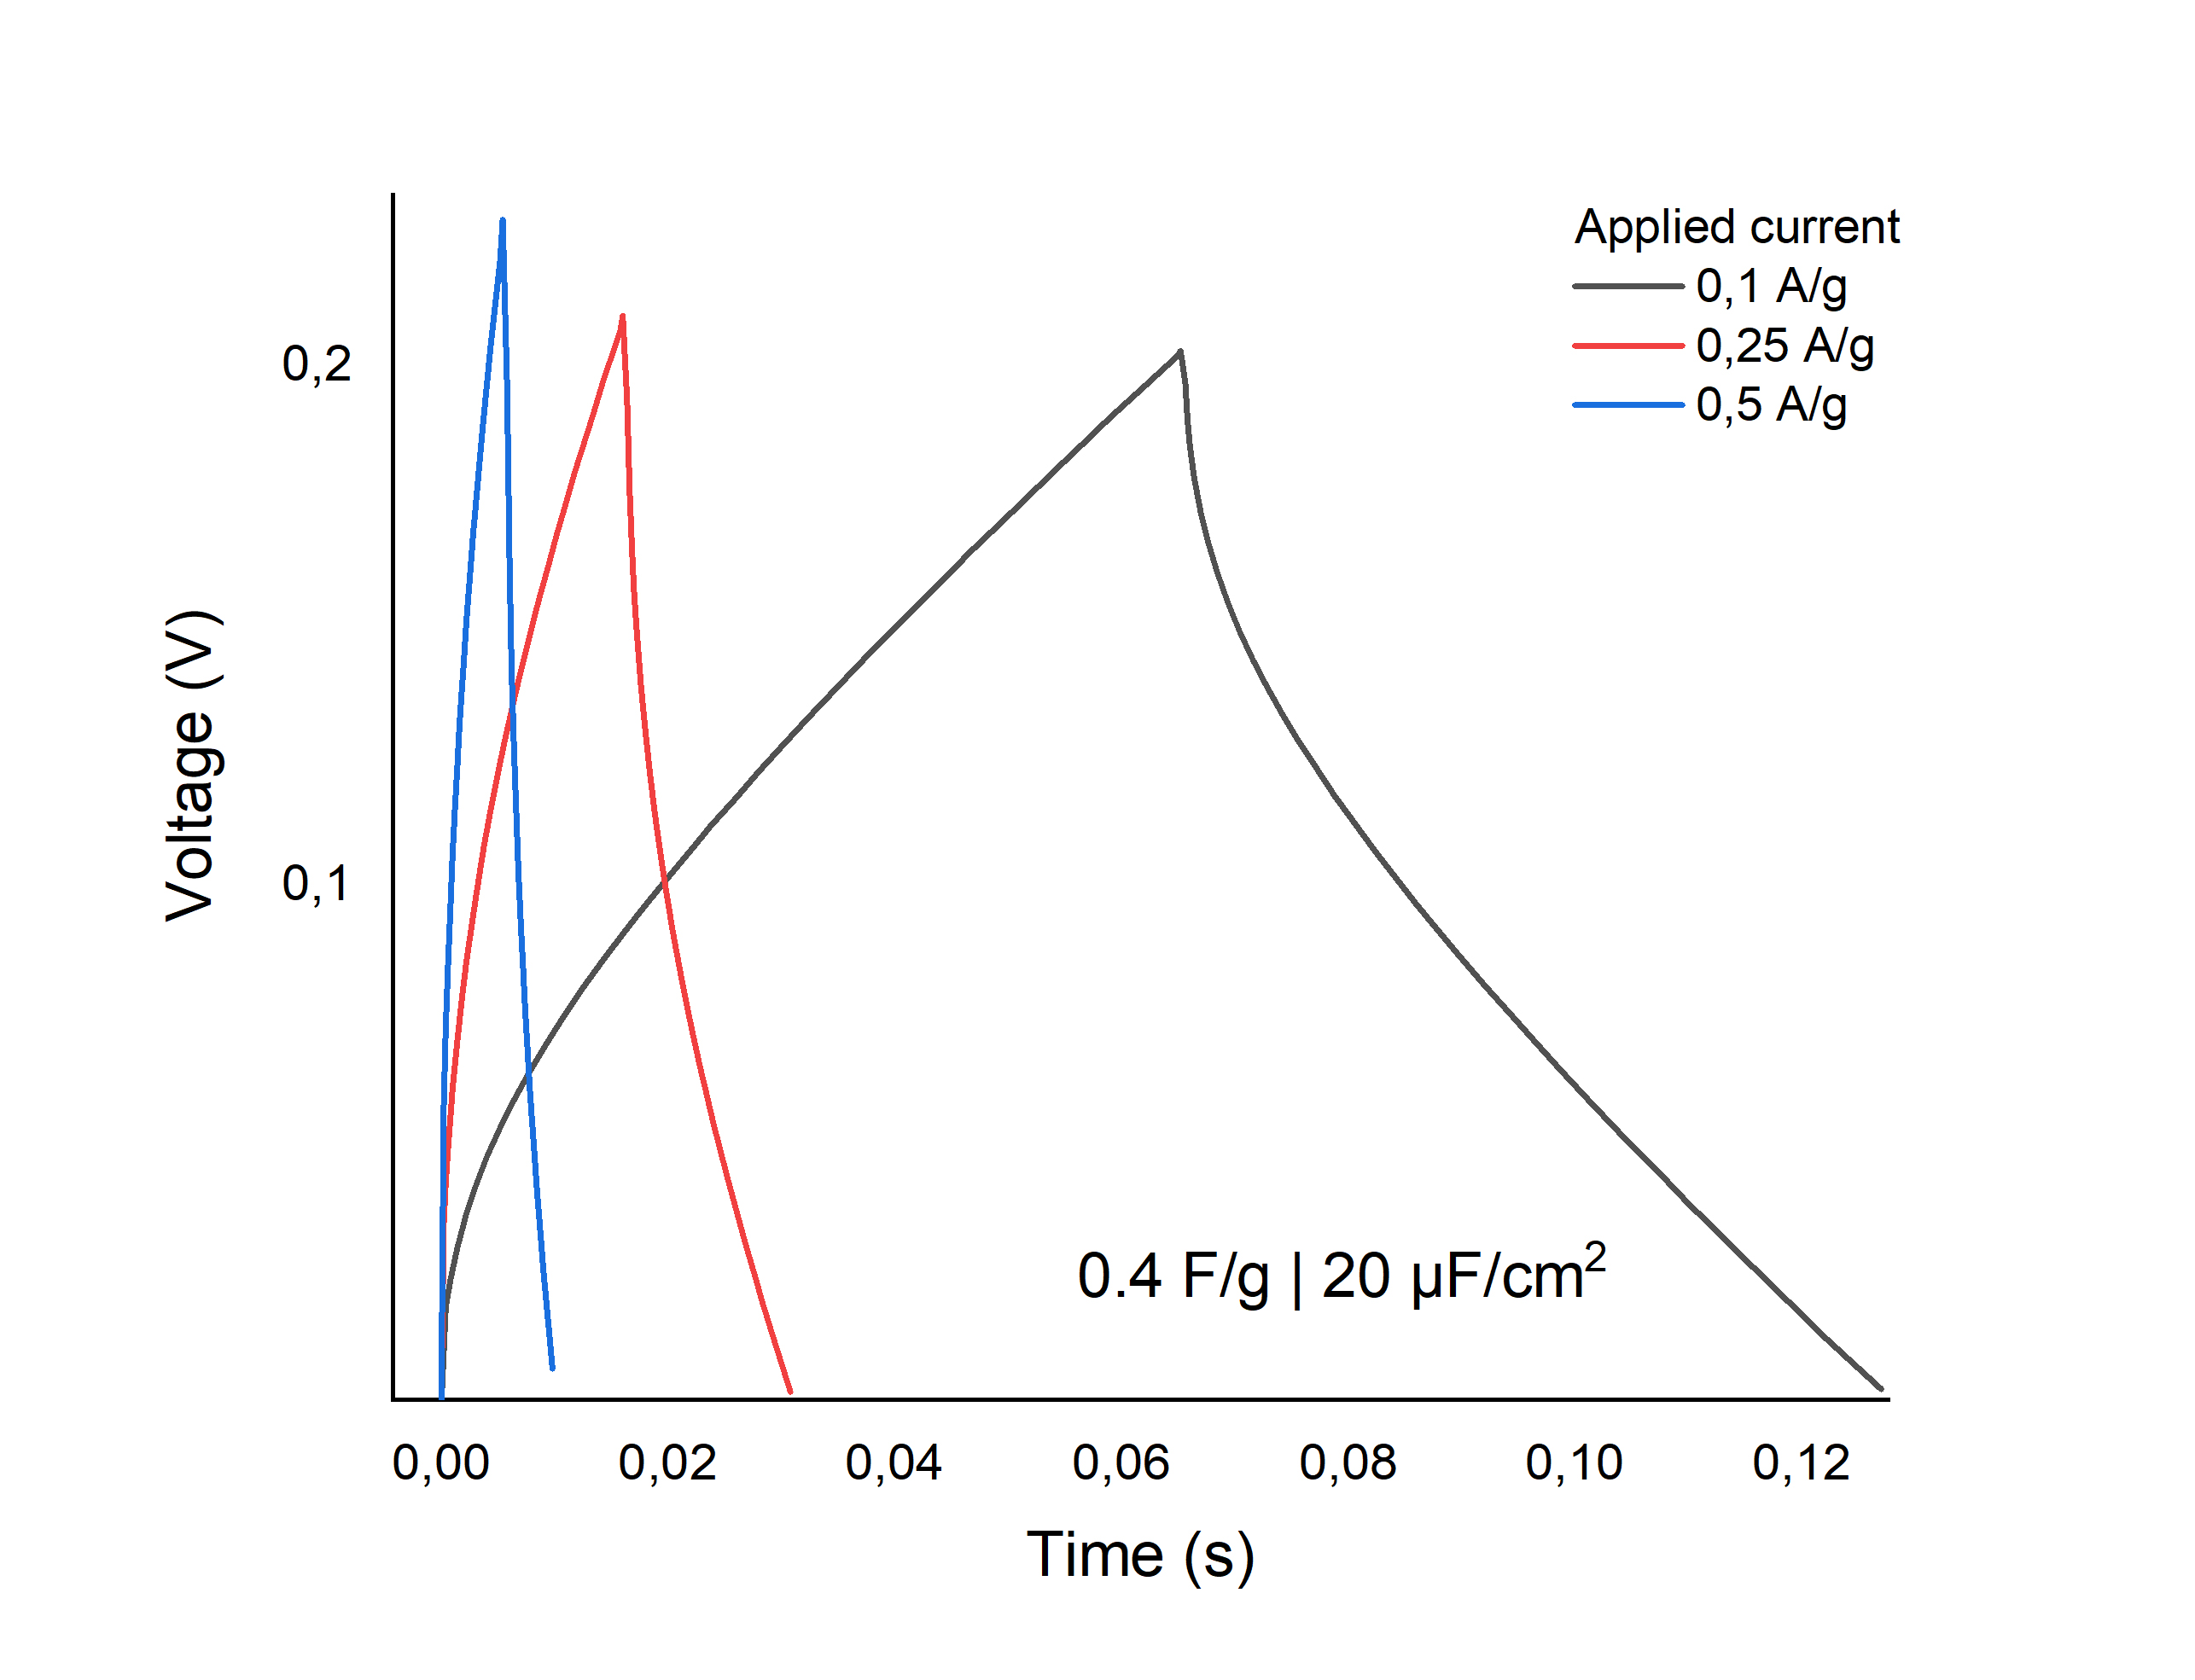
\includegraphics[width=1\textwidth]{Figures/Results/Electrochemistry/LIGF-PDMS-NaNO3-Swagelok/Cell2/GCPL_V02_Cell2.jpg}
\captionsetup{width=0.9\linewidth}
\caption{CC diagrams for $V_{max}$=0.2 V at various current densities}
\label{fig:LIGF-PDMS-cell2-CC02}
\end{subfigure}
\medskip
\caption{LIGF-PDMS Electrodes, Cell 2. CV and GCPL data in the low voltage range 0 - 0.2 V}
\label{fig:LIGF-PDMS-cell2-02}
\end{figure}

The distortions in CC curves could be a sign for Faradaic reactions taking place on the electrodes as well as of high inner resistance, which is undesirable for supercapacitor cells. On the other hand the value of iR had further increased, as compared to LIGF-Kapton electrodes. The discharging branch of the curves did not show a characteristic for the previous cases kink at the bottom of an iR drop which made the linear fit, needed for capacitance estimations, more difficult and most probably less accurate. 

\begin{figure}[H]
\begin{subfigure}{0.49\textwidth}
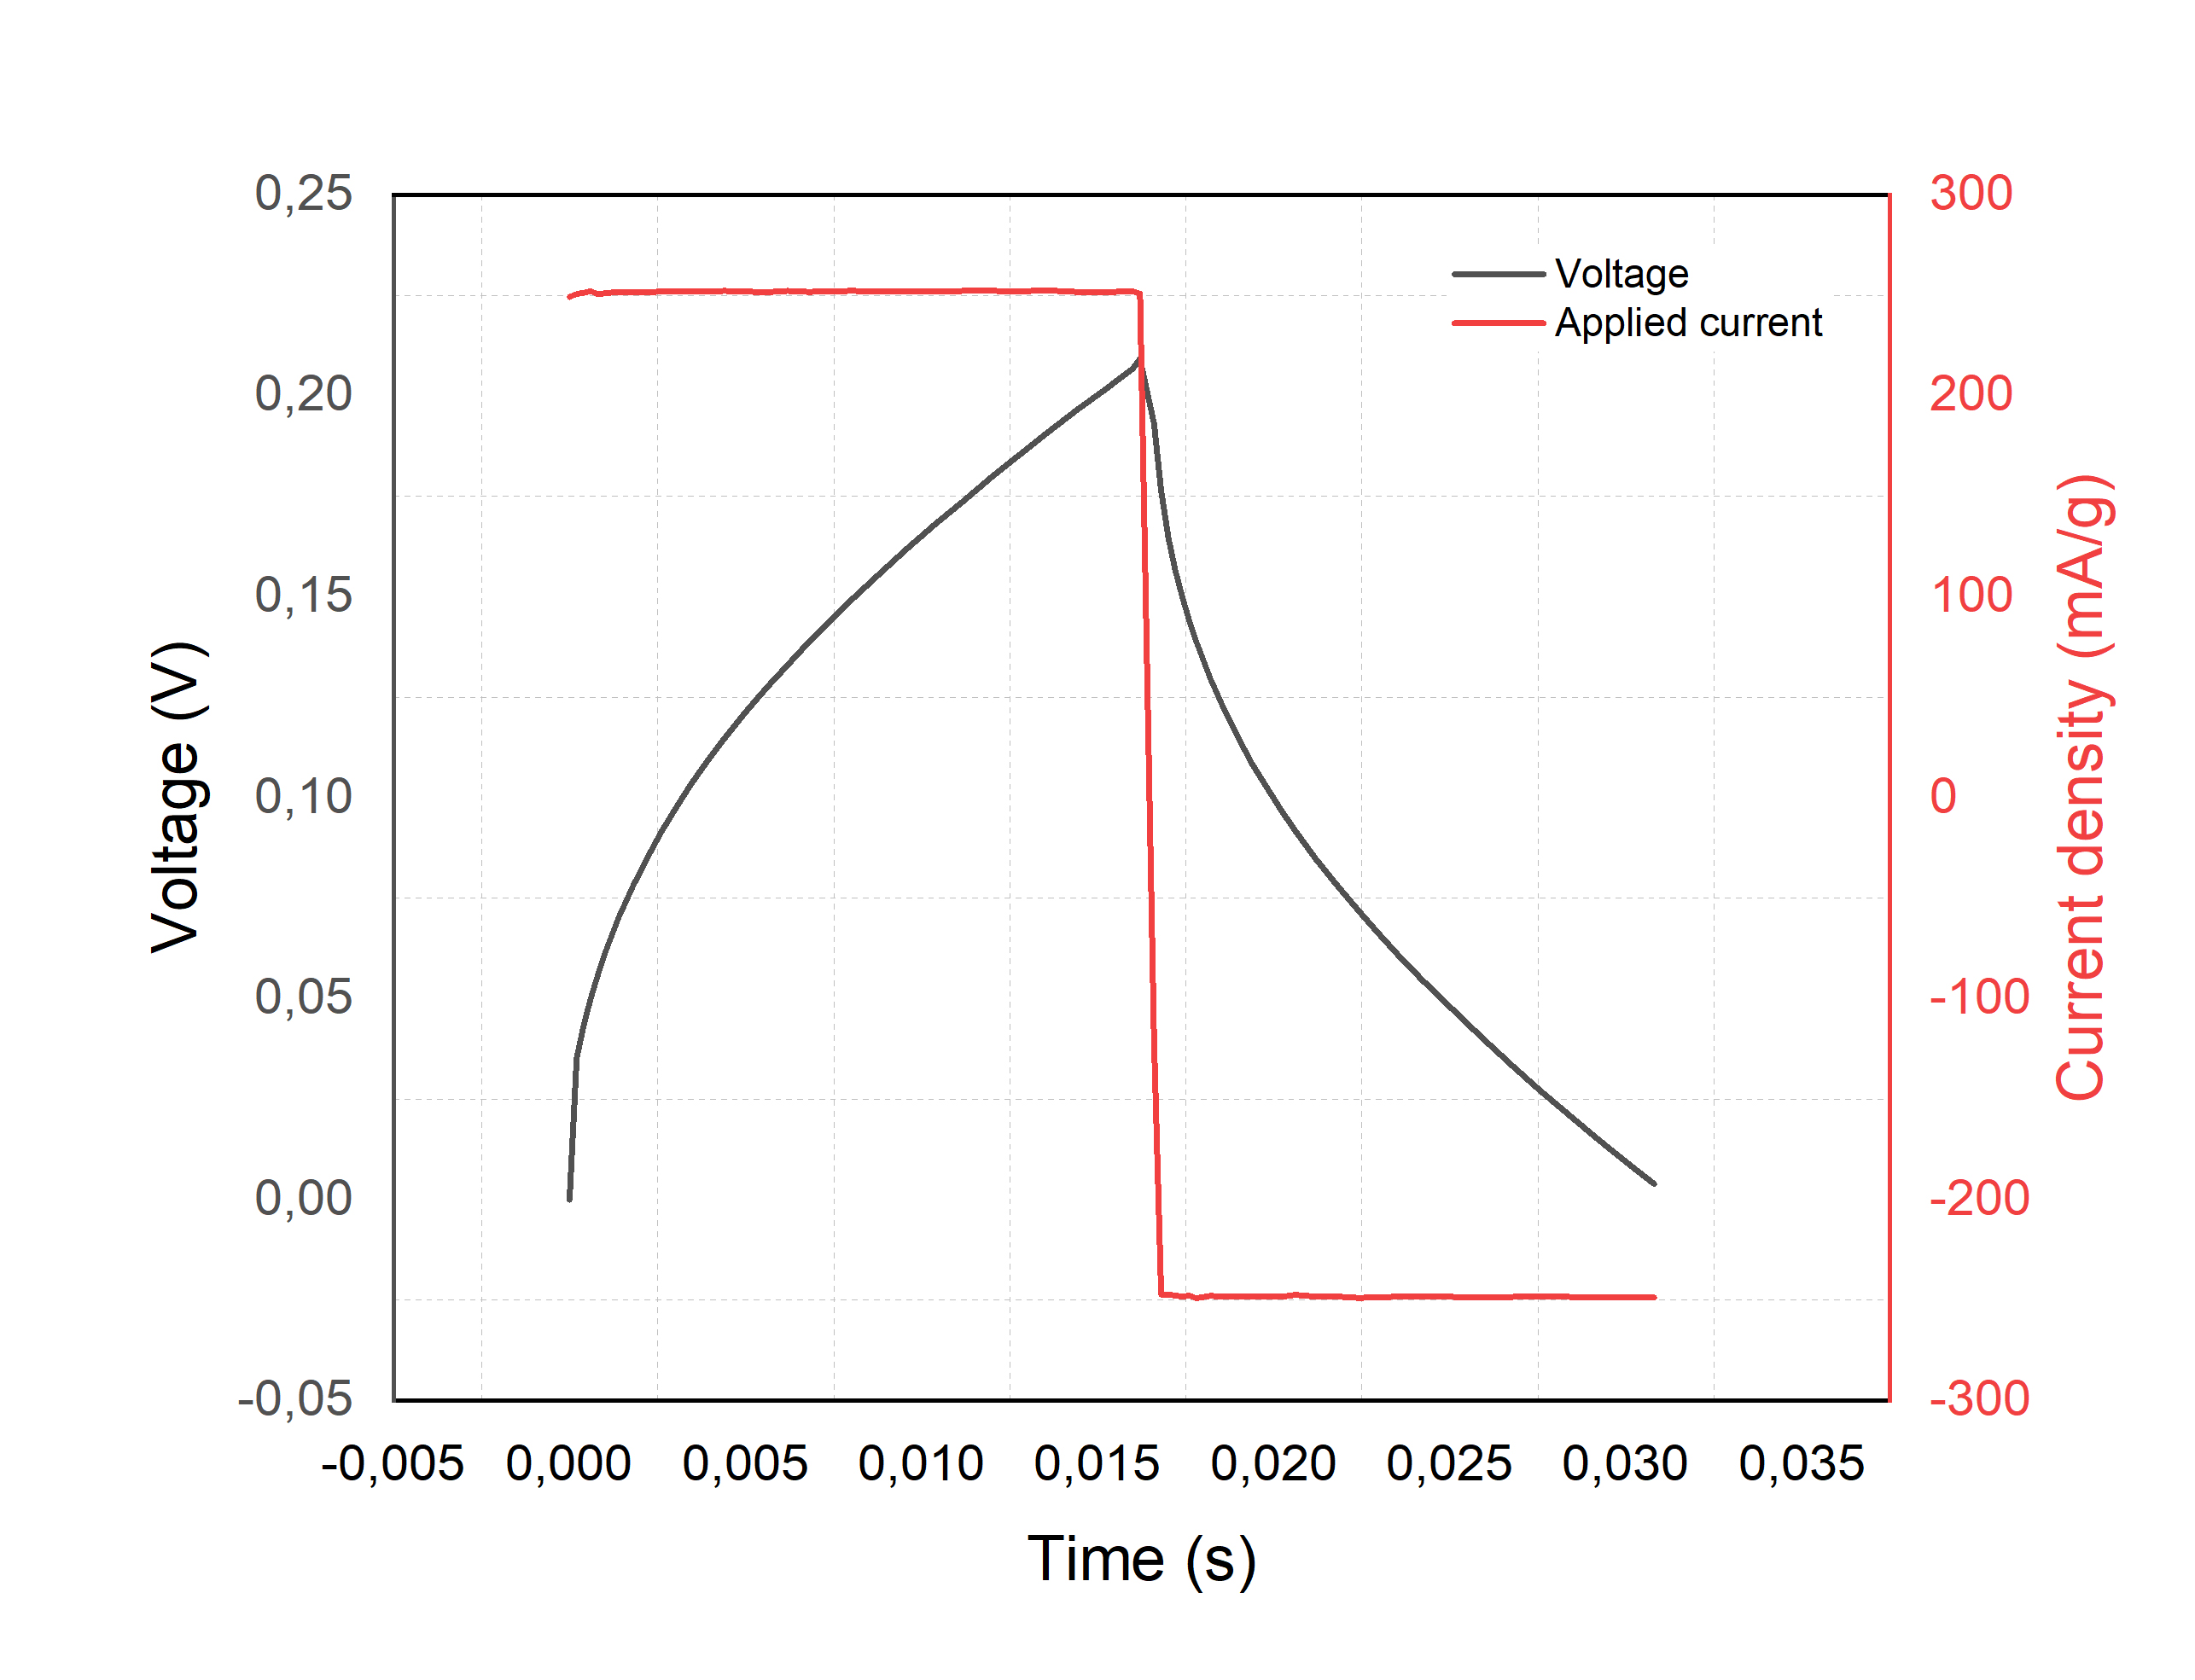
\includegraphics[width=1\textwidth]{Figures/Results/Electrochemistry/LIGF-PDMS-NaNO3-Swagelok/Cell2/GCPL_025A_cell2.jpg} 
\captionsetup{width=0.9\linewidth}
\caption{LIGF-PDMS Electrodes, Cell 2. Galvanostatic charge-discharge cycle up to $V_{max}=0.2\:V$ at 250 mA/g}
\label{fig:LIG-PDMS-cell2-CC-12}
\end{subfigure}
\begin{subfigure}{0.49\textwidth}
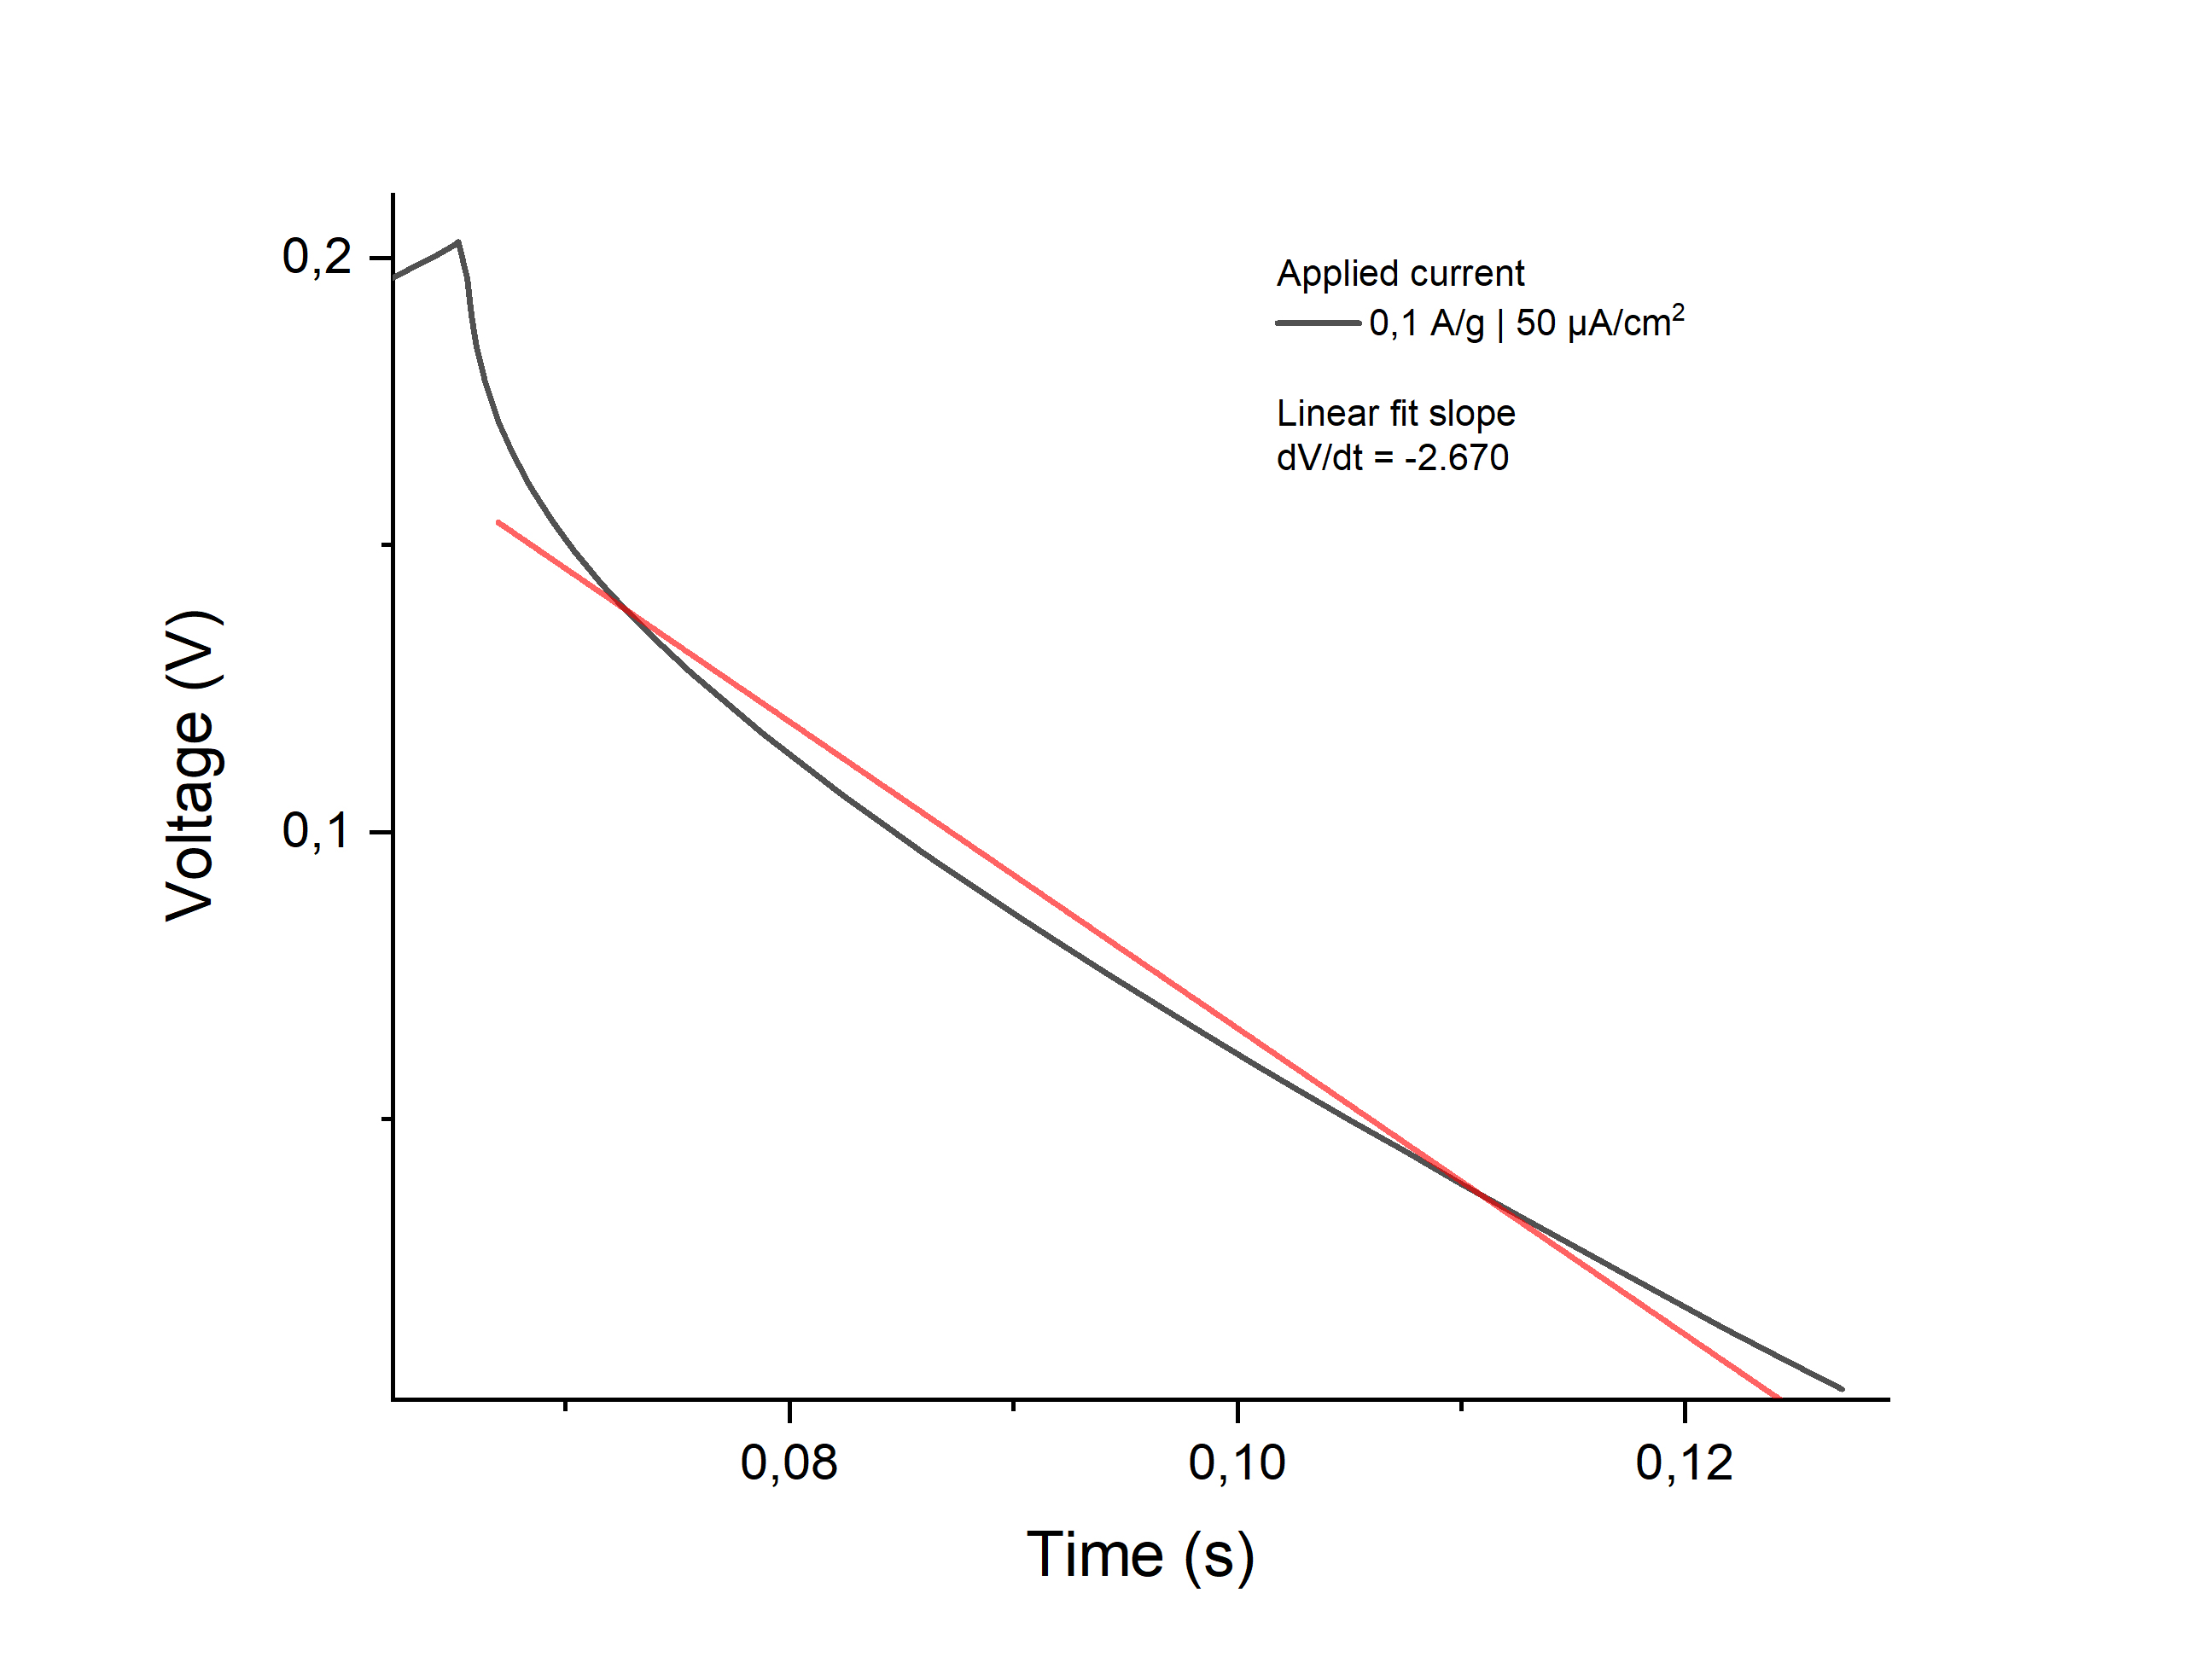
\includegraphics[width=1\textwidth]{Figures/Results/Electrochemistry/LIGF-PDMS-NaNO3-Swagelok/Cell2/GCPL_V02_Cs_Calc_fit_Cell2.jpg}
\captionsetup{width=0.9\linewidth}
\caption{Towards determination of the slope of a discharge branch of a CC curve for capacitance evaluation}
\label{fig:cc-slope-determination-2}
\end{subfigure}
\medskip
\caption{LIGF-PDMS Electrodes in Swagelok Cell 2. Distorted CC curves}
\label{fig:LIGF-PDMS-CC-12}
\end{figure}

Further cyclic voltammetry attempts for larger voltage windows have delivered rather distorted CV curves which could not be used for capacitance evaluations. However, the CC $V(t)$ graphs did not deteriorate more than they were and showed the same shape for all cycles measured at $V_{max}$ from 0.2 to 0.5\:V:

\begin{figure}[H]
\begin{subfigure}{0.49\textwidth}
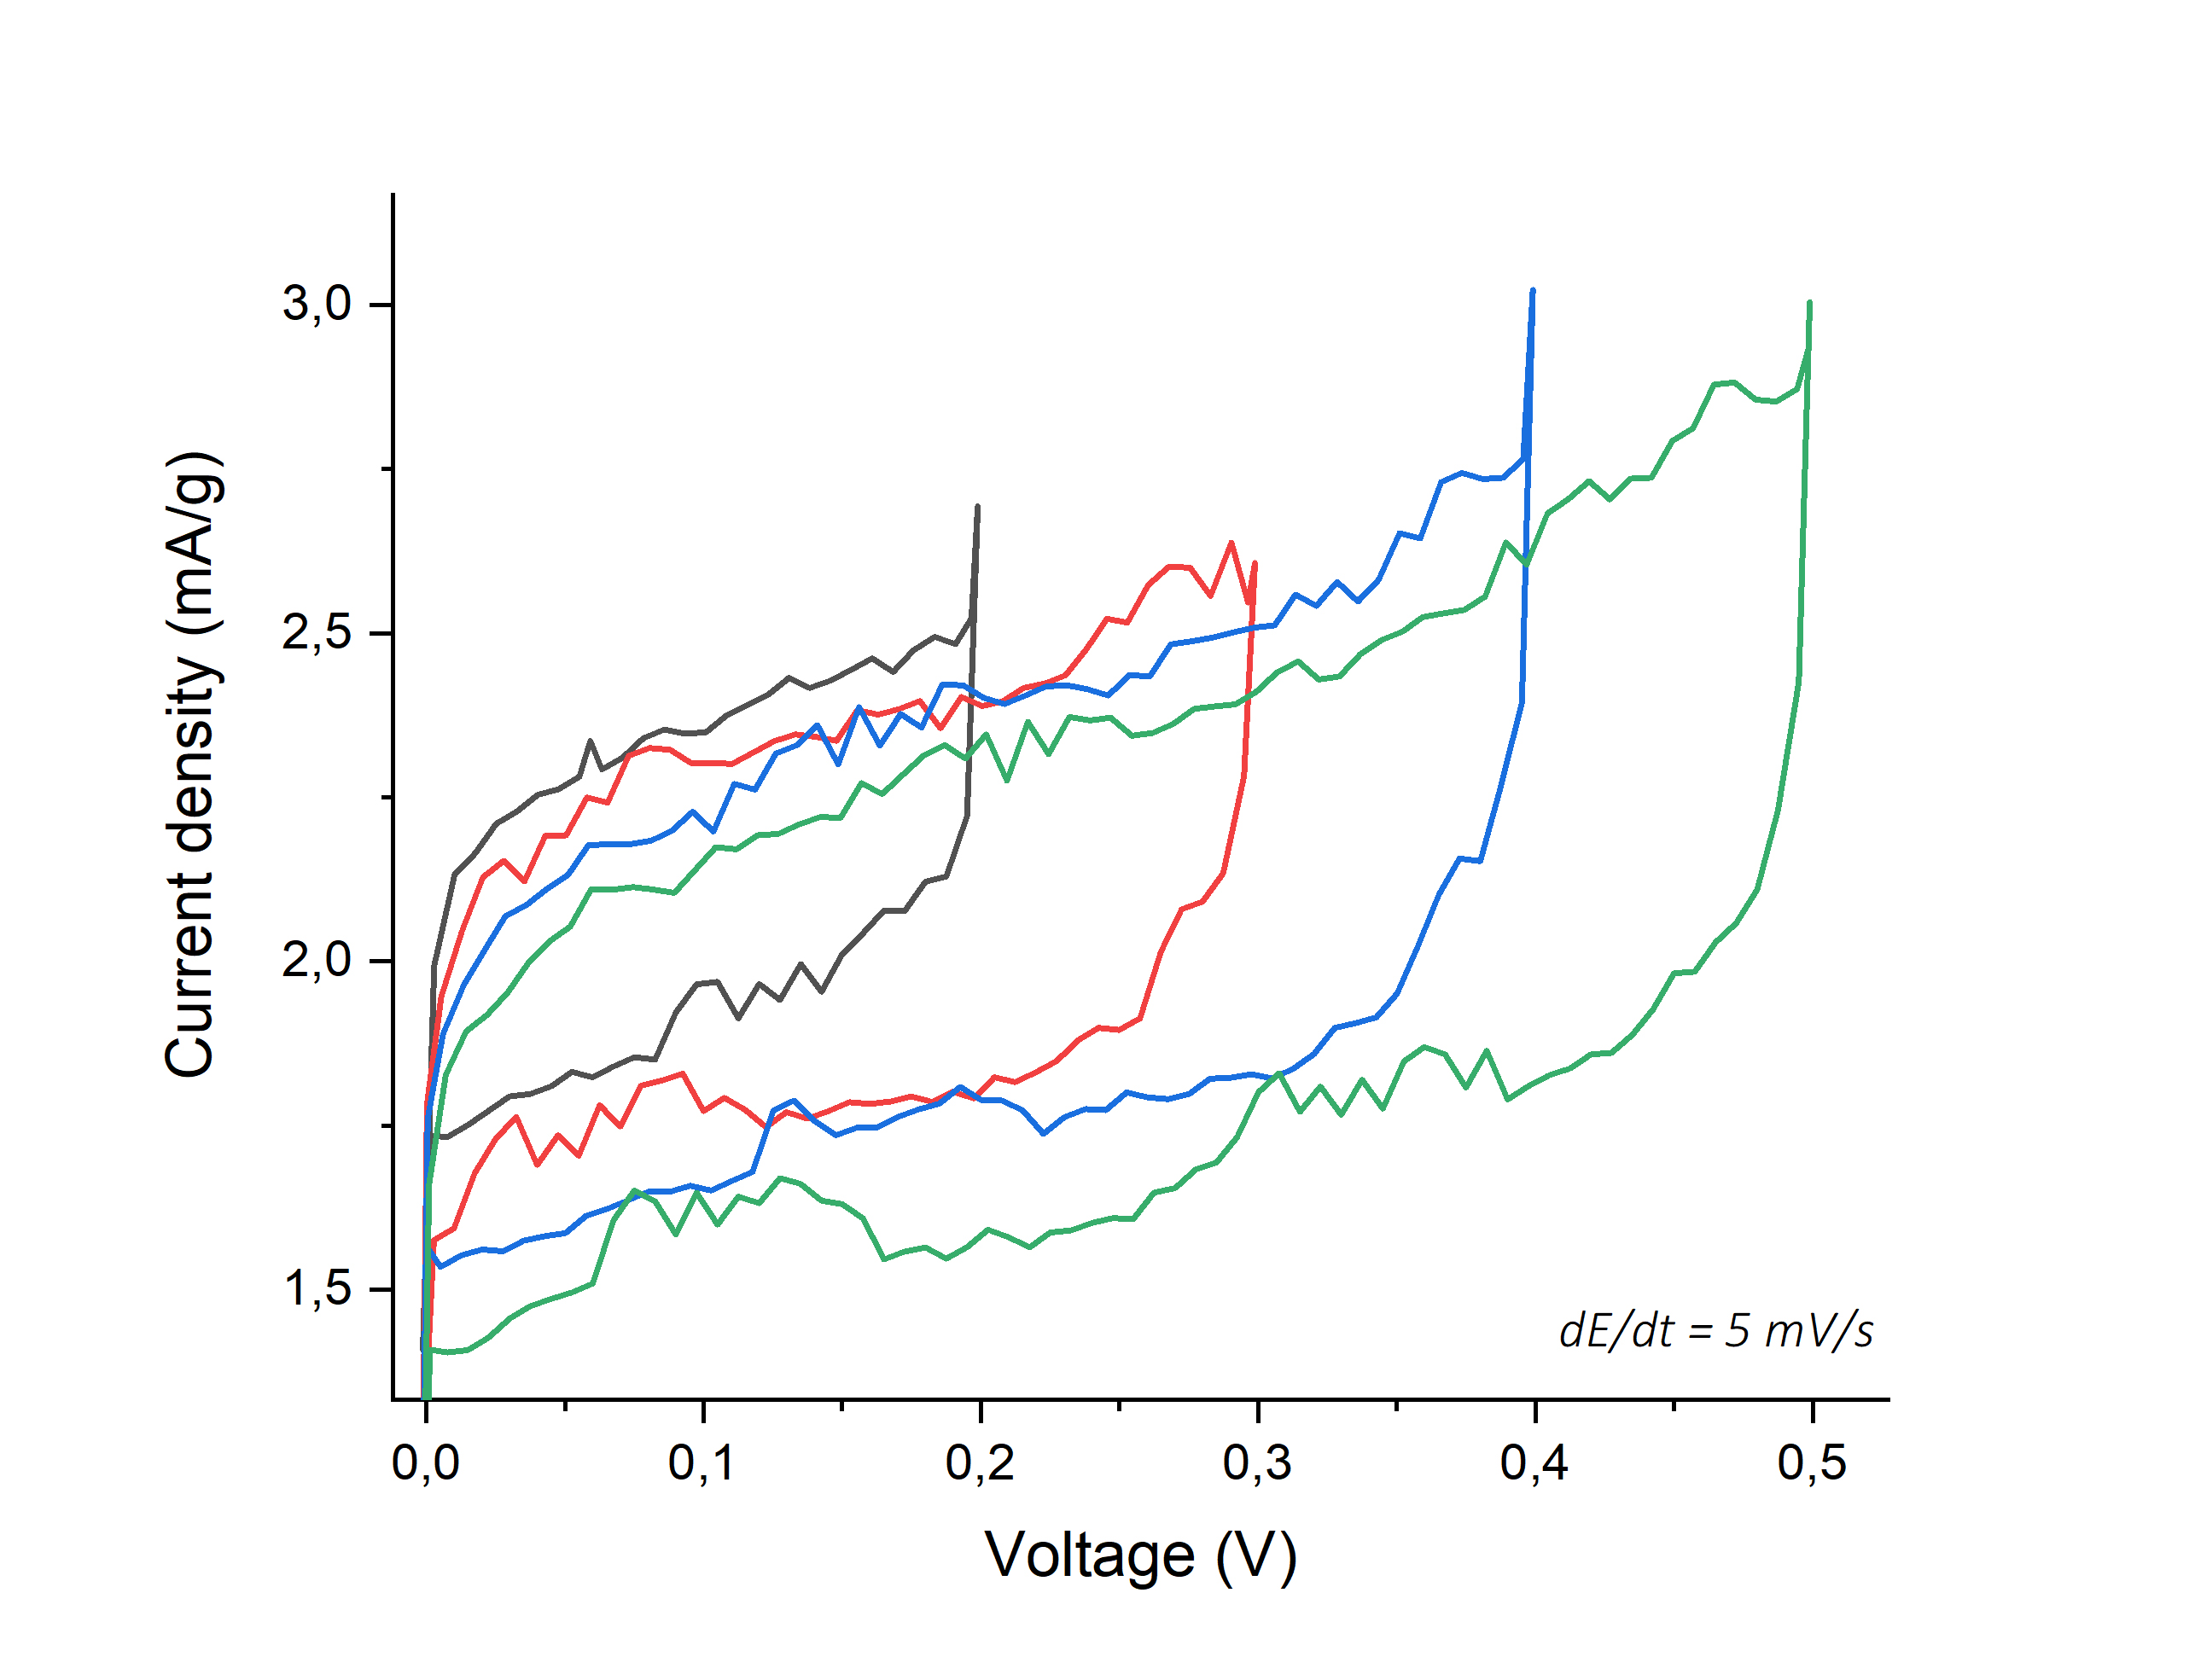
\includegraphics[width=1\textwidth]{Figures/Results/Electrochemistry/LIGF-PDMS-NaNO3-Swagelok/Cell2/CV-high-voltage.jpg} 
\captionsetup{width=0.9\linewidth}
\caption{CV diagrams at $\Delta V$ = 0.2$\div$0.5\:V for 5\:mV/s scan rate}
\label{fig:LIGF-PDMS-cell2-CV06}
\end{subfigure}
\begin{subfigure}{0.49\textwidth}
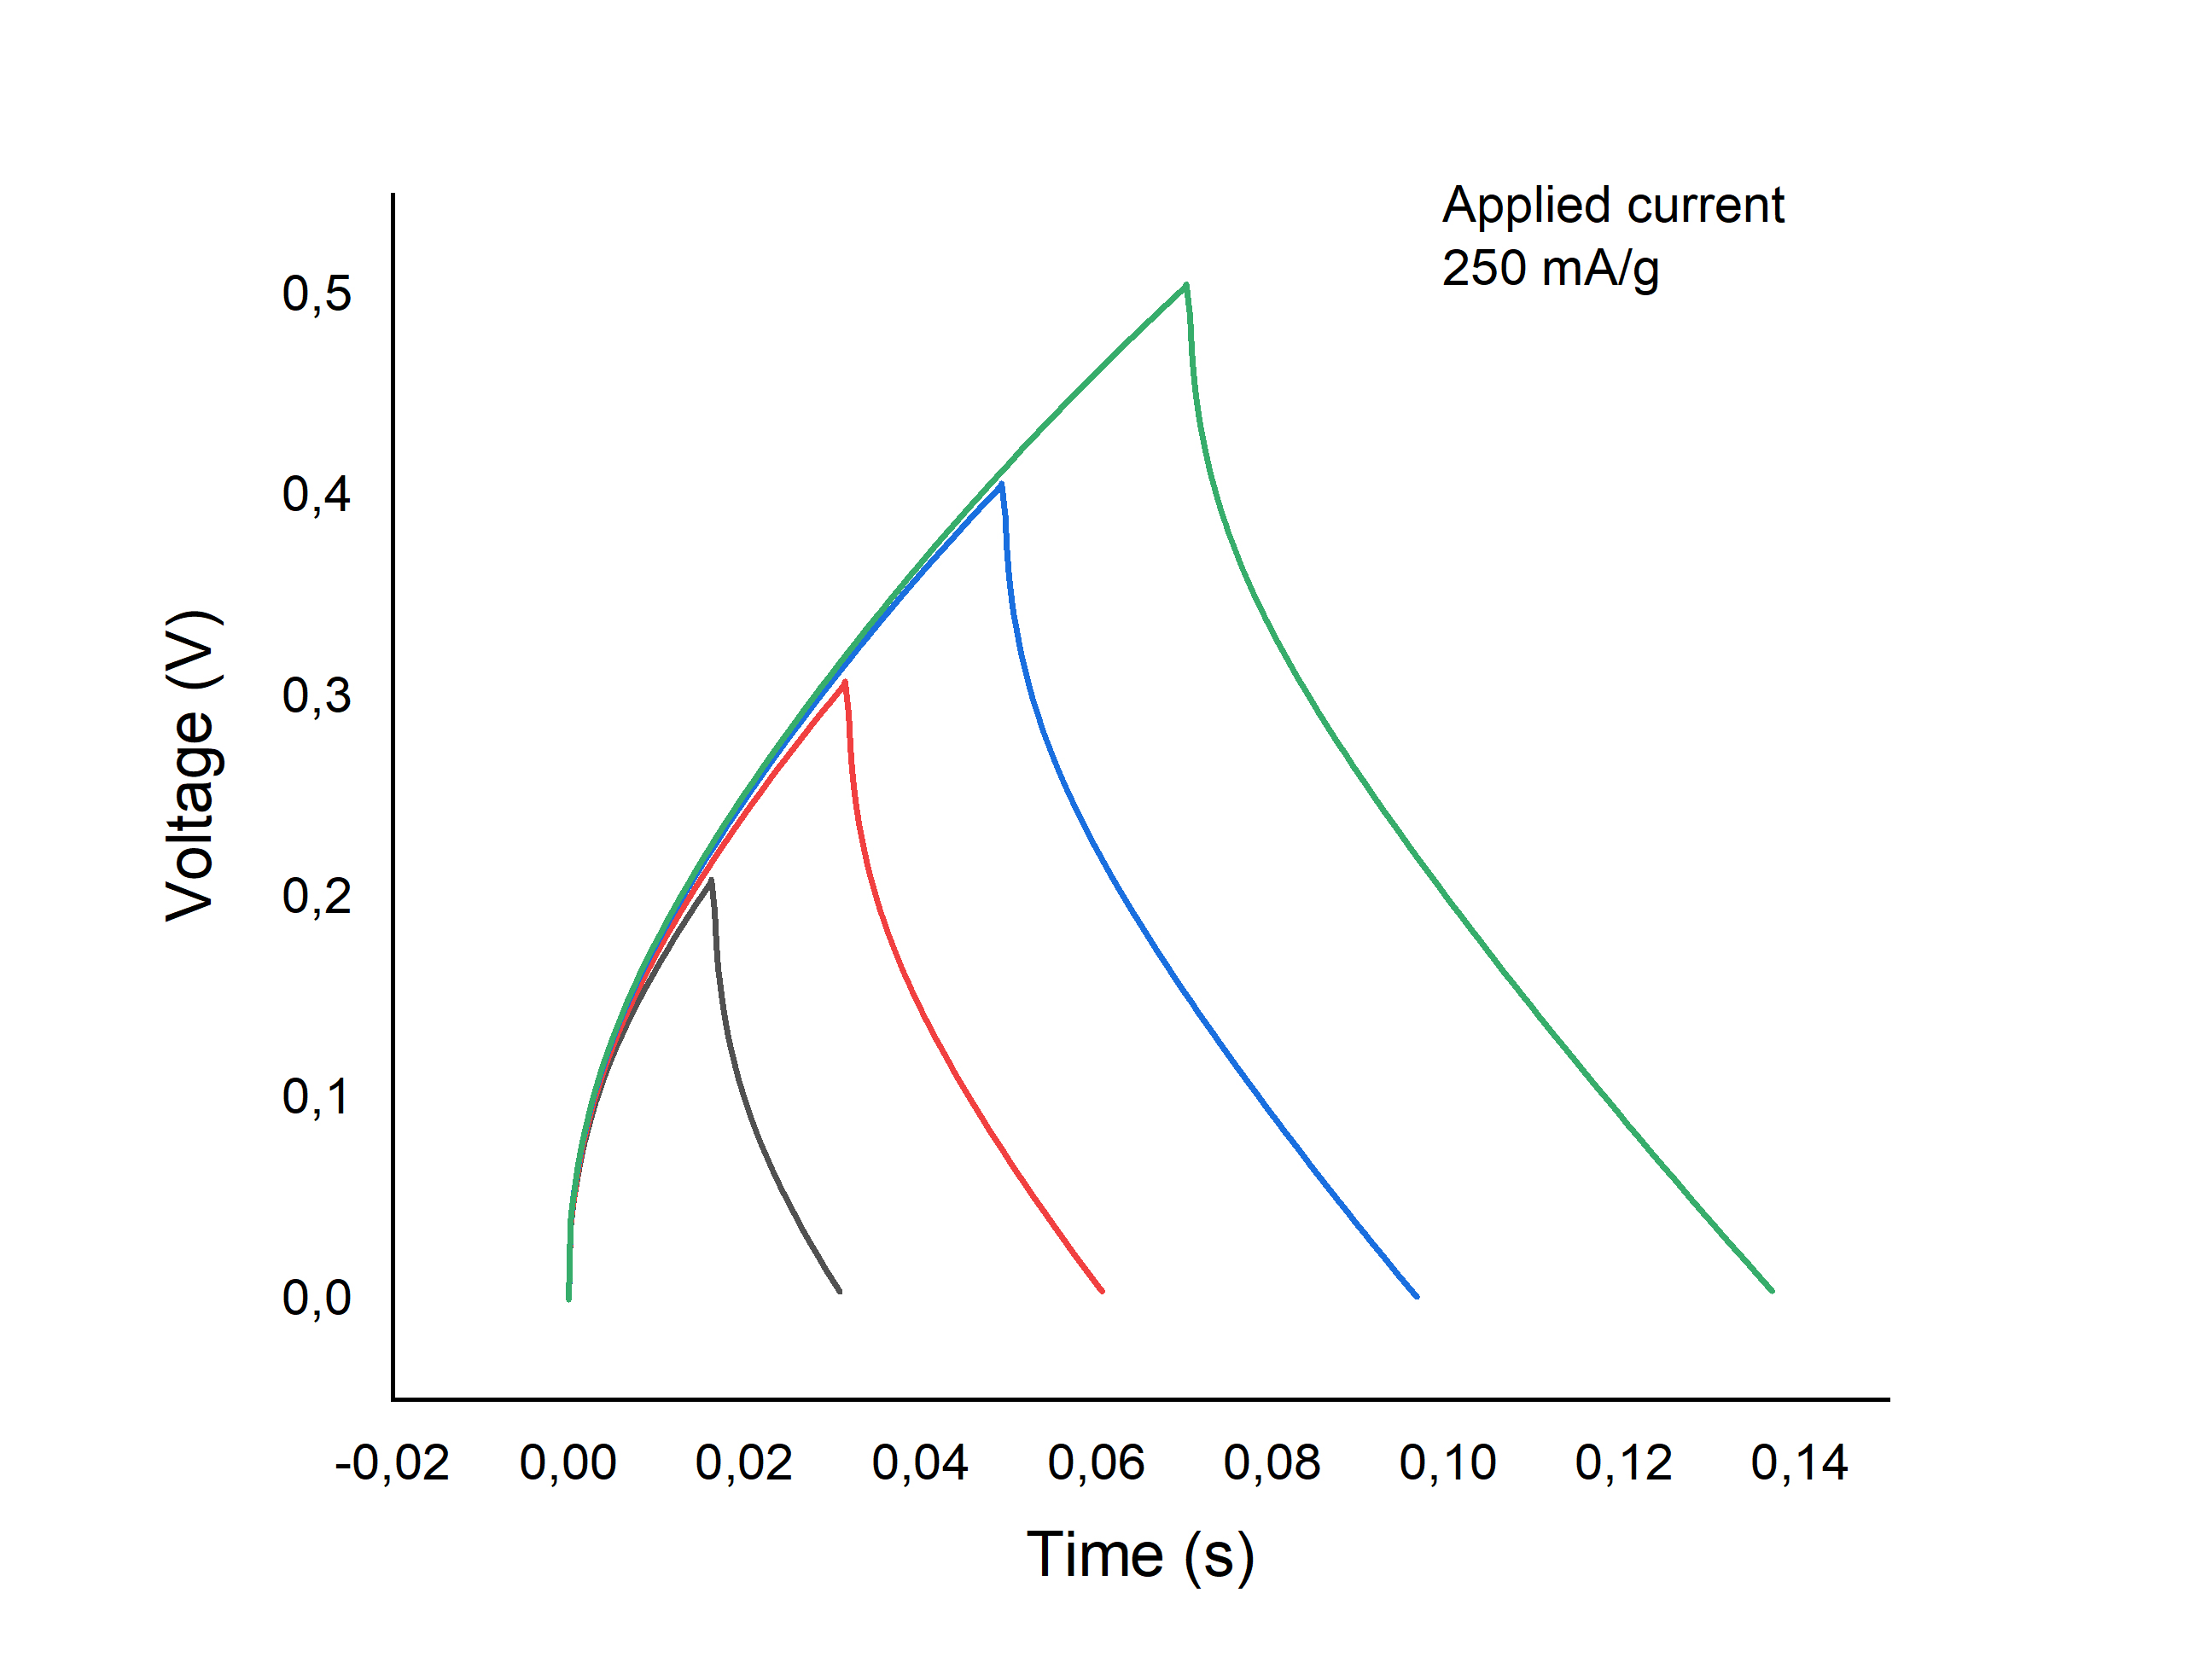
\includegraphics[width=1\textwidth]{Figures/Results/Electrochemistry/LIGF-PDMS-NaNO3-Swagelok/Cell2/GCPL_diff_V_cell2.jpg}
\captionsetup{width=0.9\linewidth}
\caption{CC diagrams for $V_{max}$=0.2$\div$0.5\:V at constant current densities}
\label{fig:LIGF-PDMS-cell2-CC06}
\end{subfigure}
\medskip
\caption{LIGF-PDMS Electrodes, Cell 2. CV and GCPL data in the voltage range 0\:-\:0.5\:V}
\label{fig:LIGF-PDMS-cell2-06}
\end{figure}

\textbf{Capacitance Evaluations for LIGF-PDMS Electrodes}

The data obtained in the experiments was collected to estimate the capacitance performance of the LIGF-PDMS composite. As can be seen in the figures below, the $C_g$ and $C_A$ of the composite material were about fivefold lower than the values for LIGF-Kapton. 

\begin{figure}[H]
\centering
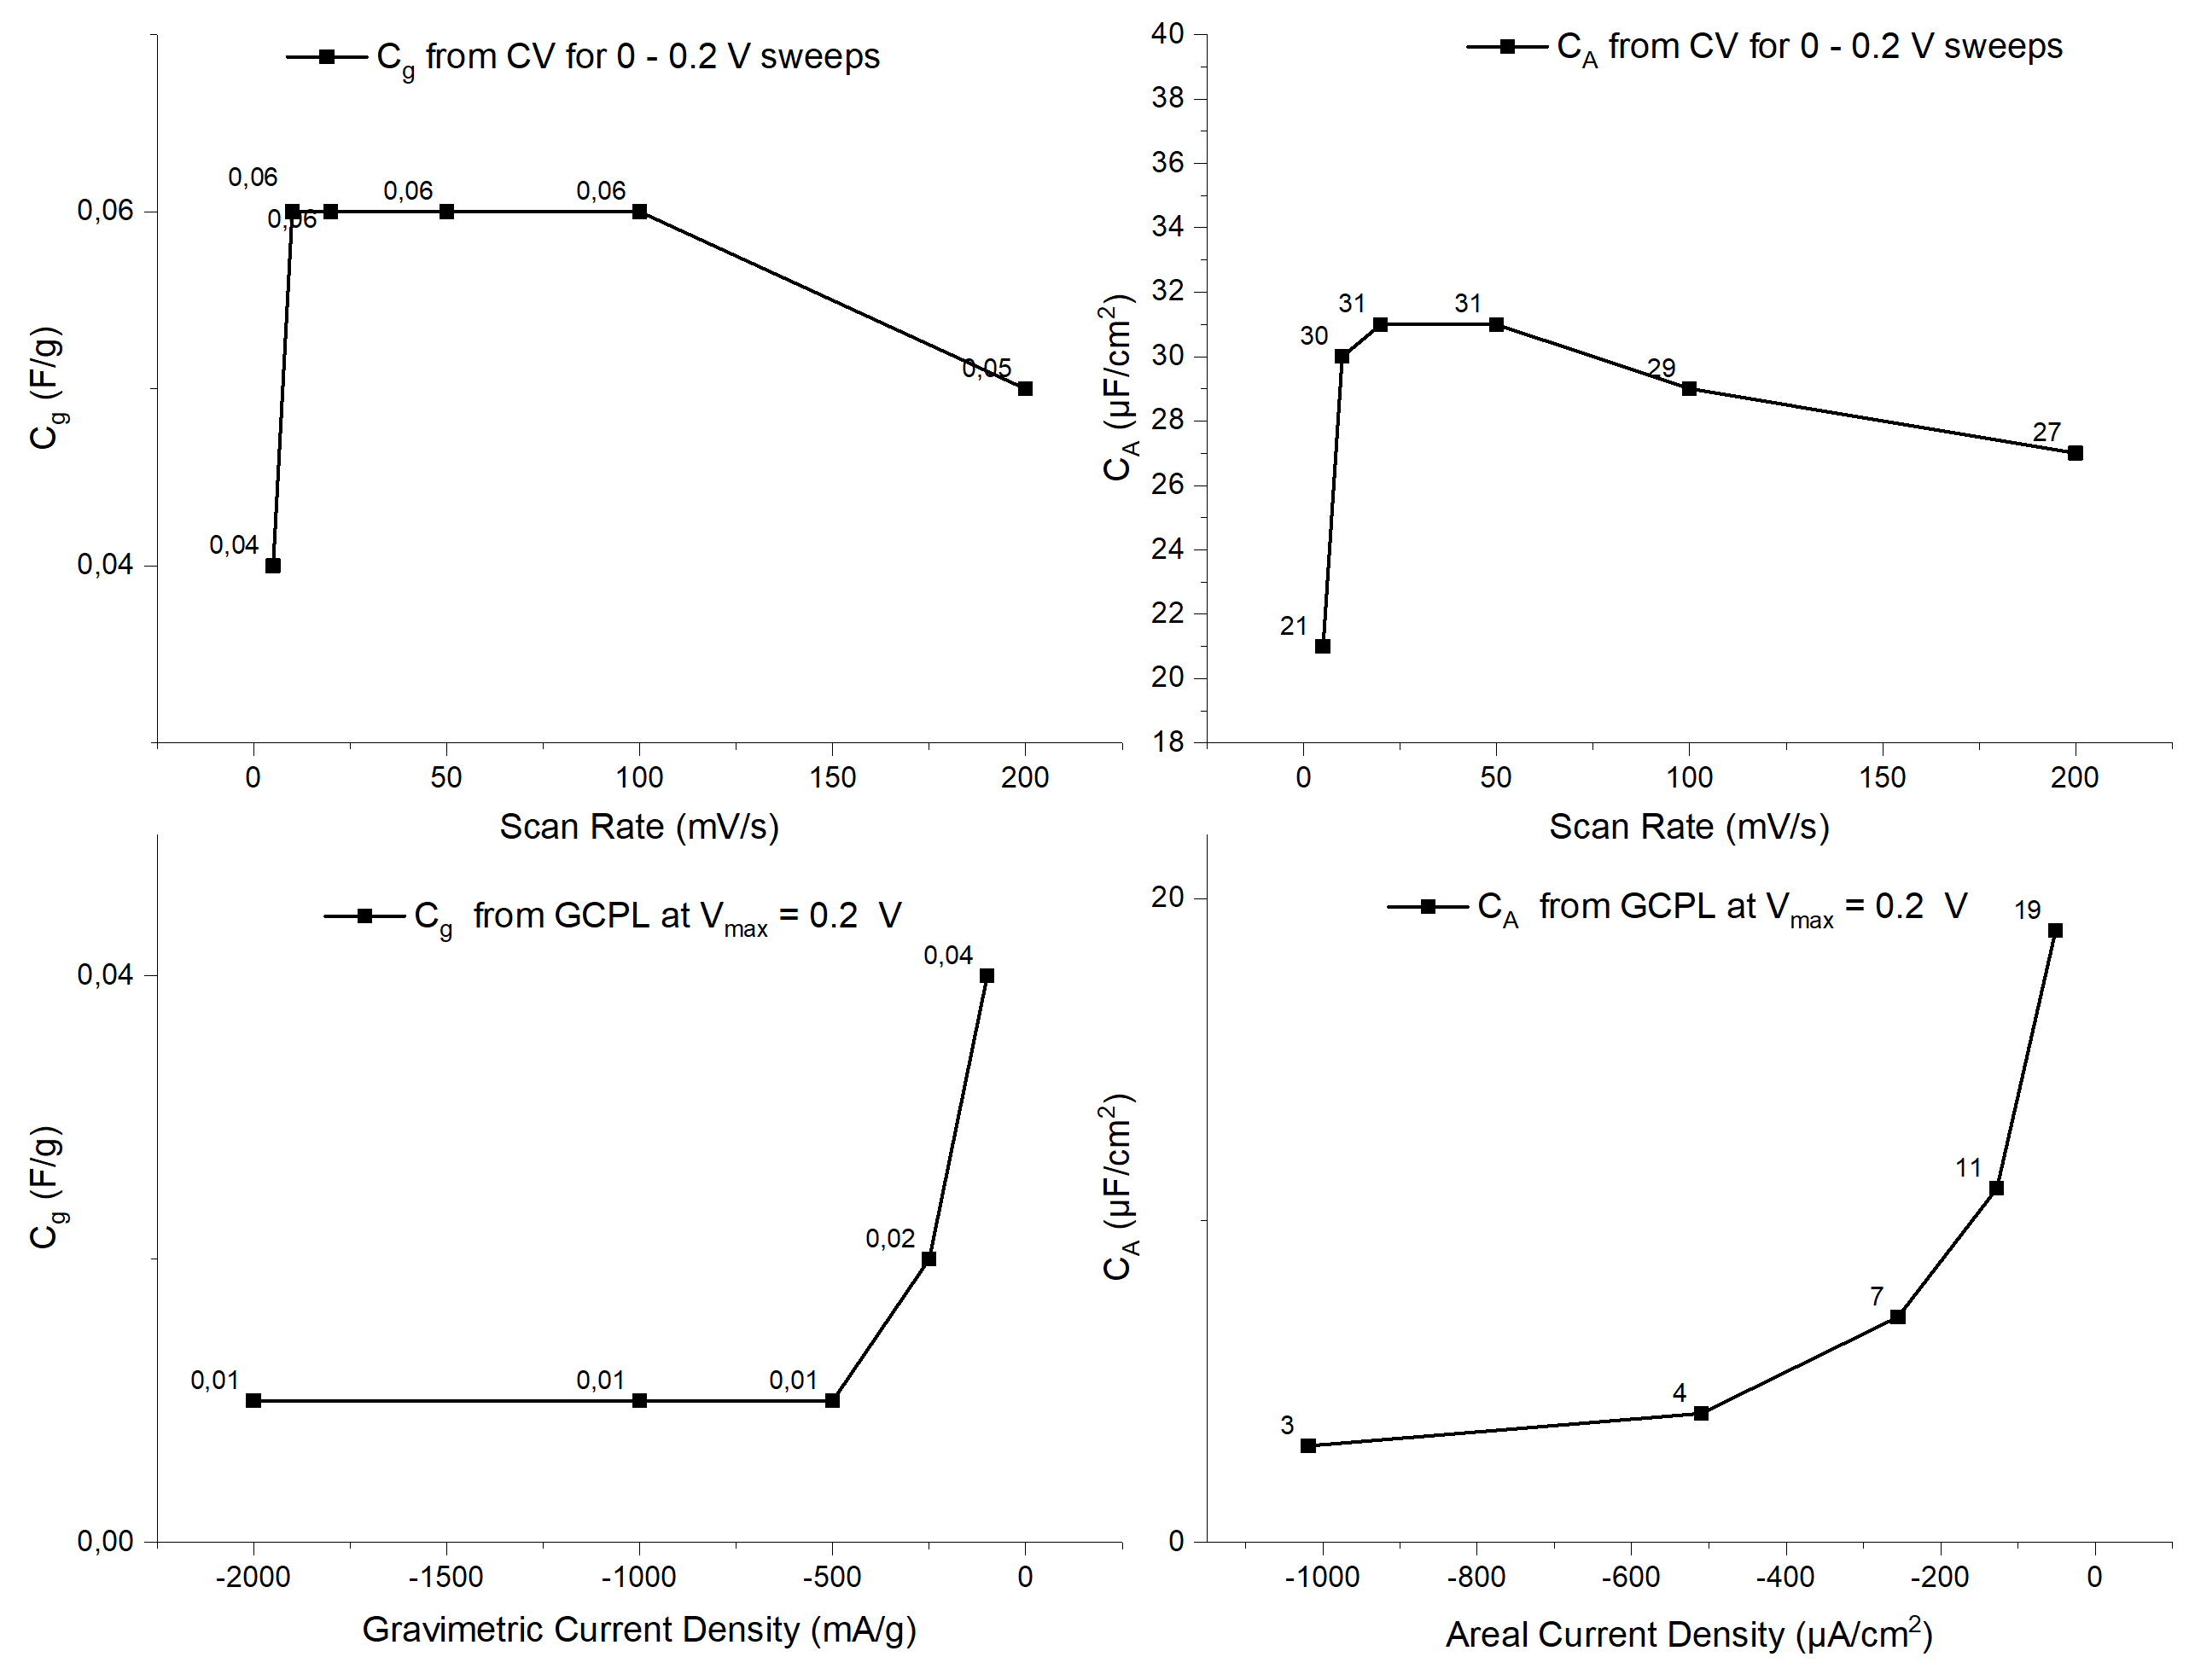
\includegraphics[width=0.9\textwidth]{Figures/Results/Electrochemistry/LIGF-PDMS-NaNO3-Swagelok/Cell2/Capacitances-4-PDMS.jpg}
\medskip
\captionsetup{width=1\linewidth}
\caption{LIGF-PDMS Electrode - specific capacitance values evaluated from CV data at voltage window of 0 - 0.2\:V for increasing scan rates $dV/dt$ (top) and from GCPL data for increasing charge-discharge current densities at fixed $V_{max}$ = 0.2\:V (bottom)}
\label{fig:LIGF-PDMS-capcitance-4}
\end{figure}

Although the calculations for $C_g$ were made with the estimation that all the LIGF formed during lasering was translated into the composite, it is in fact obvious that a substantial part of it became unavailable for the electrode function after being embedded into the dielectric polydimethylsiloxane matrix, which in turn could aggravate the fact of the lower capacitance numbers.

XXX Here the results of Francesca will help to discuss to what extent the available surface area of an electrode decreases with forming the LIG-PDMS composite.

.

\textbf{LIGP-MPU and LIGF-MPU Composite Electrodes in a Swagelok Cell}

As the fourth step in the electrochemical investigations of LIG-based SCs the ultra-thin 40 $\mu m$ LIG-MPU electrodes were tested for both types of graphene material: LIGP and LIGF, Type 4 and Type 5 in the reference Table \ref{tab:supercapacitor_electrodes} respectively. 

One Swagelok cell filled with 1M NaNO$_3$ electrolyte was assembled for each electrode variation. Cyclic voltammetry tests were performed at constant scan rate of 2\:mV/s for four sweep windows of 0 - 0.1\:V, 0.1 - 0.2\:V, 0 - 0.3\:V and 0 - 0.4 V. Galvanostatic charge-discharge cycles were performed at constant current density of 100 mA/g for four $V_{max}$ values increasing with a step of 0.1\:V from 0.1 to 0.4\:V. Below are the CV diagrams obtained for the both cell Types:

\begin{figure}[H]
\begin{subfigure}{0.49\textwidth}
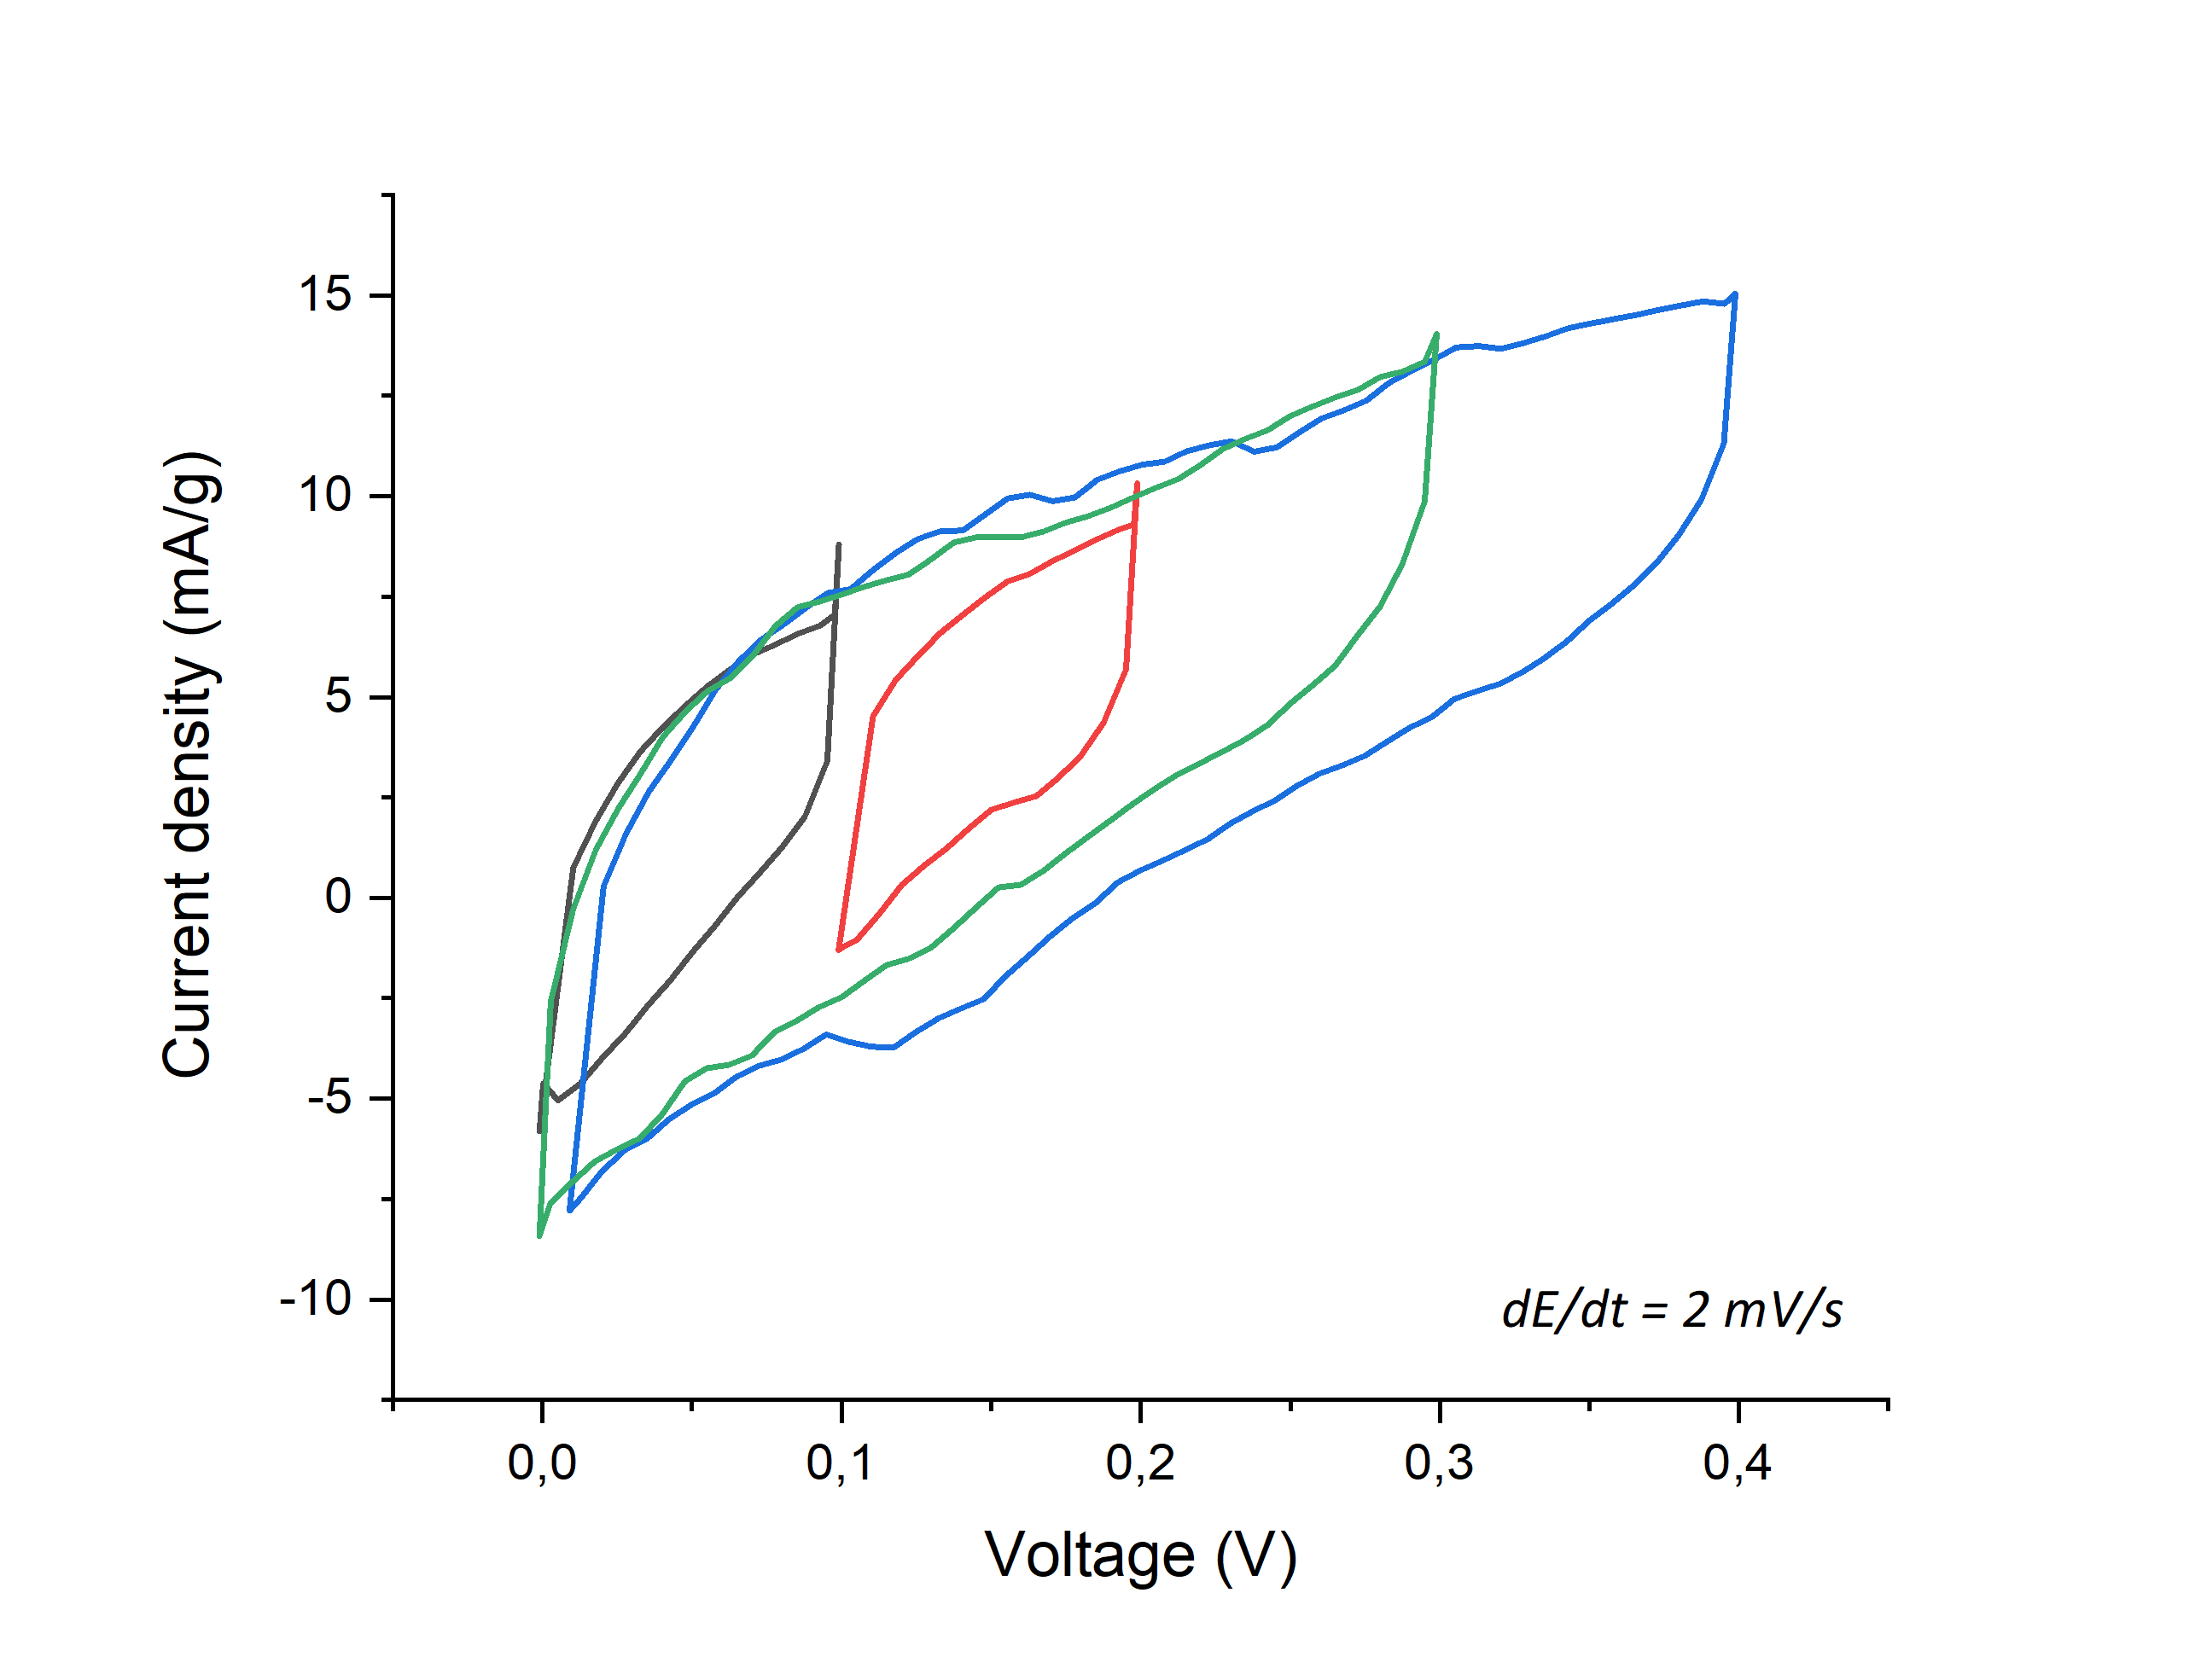
\includegraphics[width=1\textwidth]{Figures/Results/Electrochemistry/LIGP-MPU-NaNO3-Swagelok/Cell1/CV-different-windows.jpg} 
\captionsetup{width=0.9\linewidth}
\caption{LIGP-MPU Electrodes, Cell 1}
\label{fig:LIGP-MPU-cell1}
\end{subfigure}
\begin{subfigure}{0.49\textwidth}
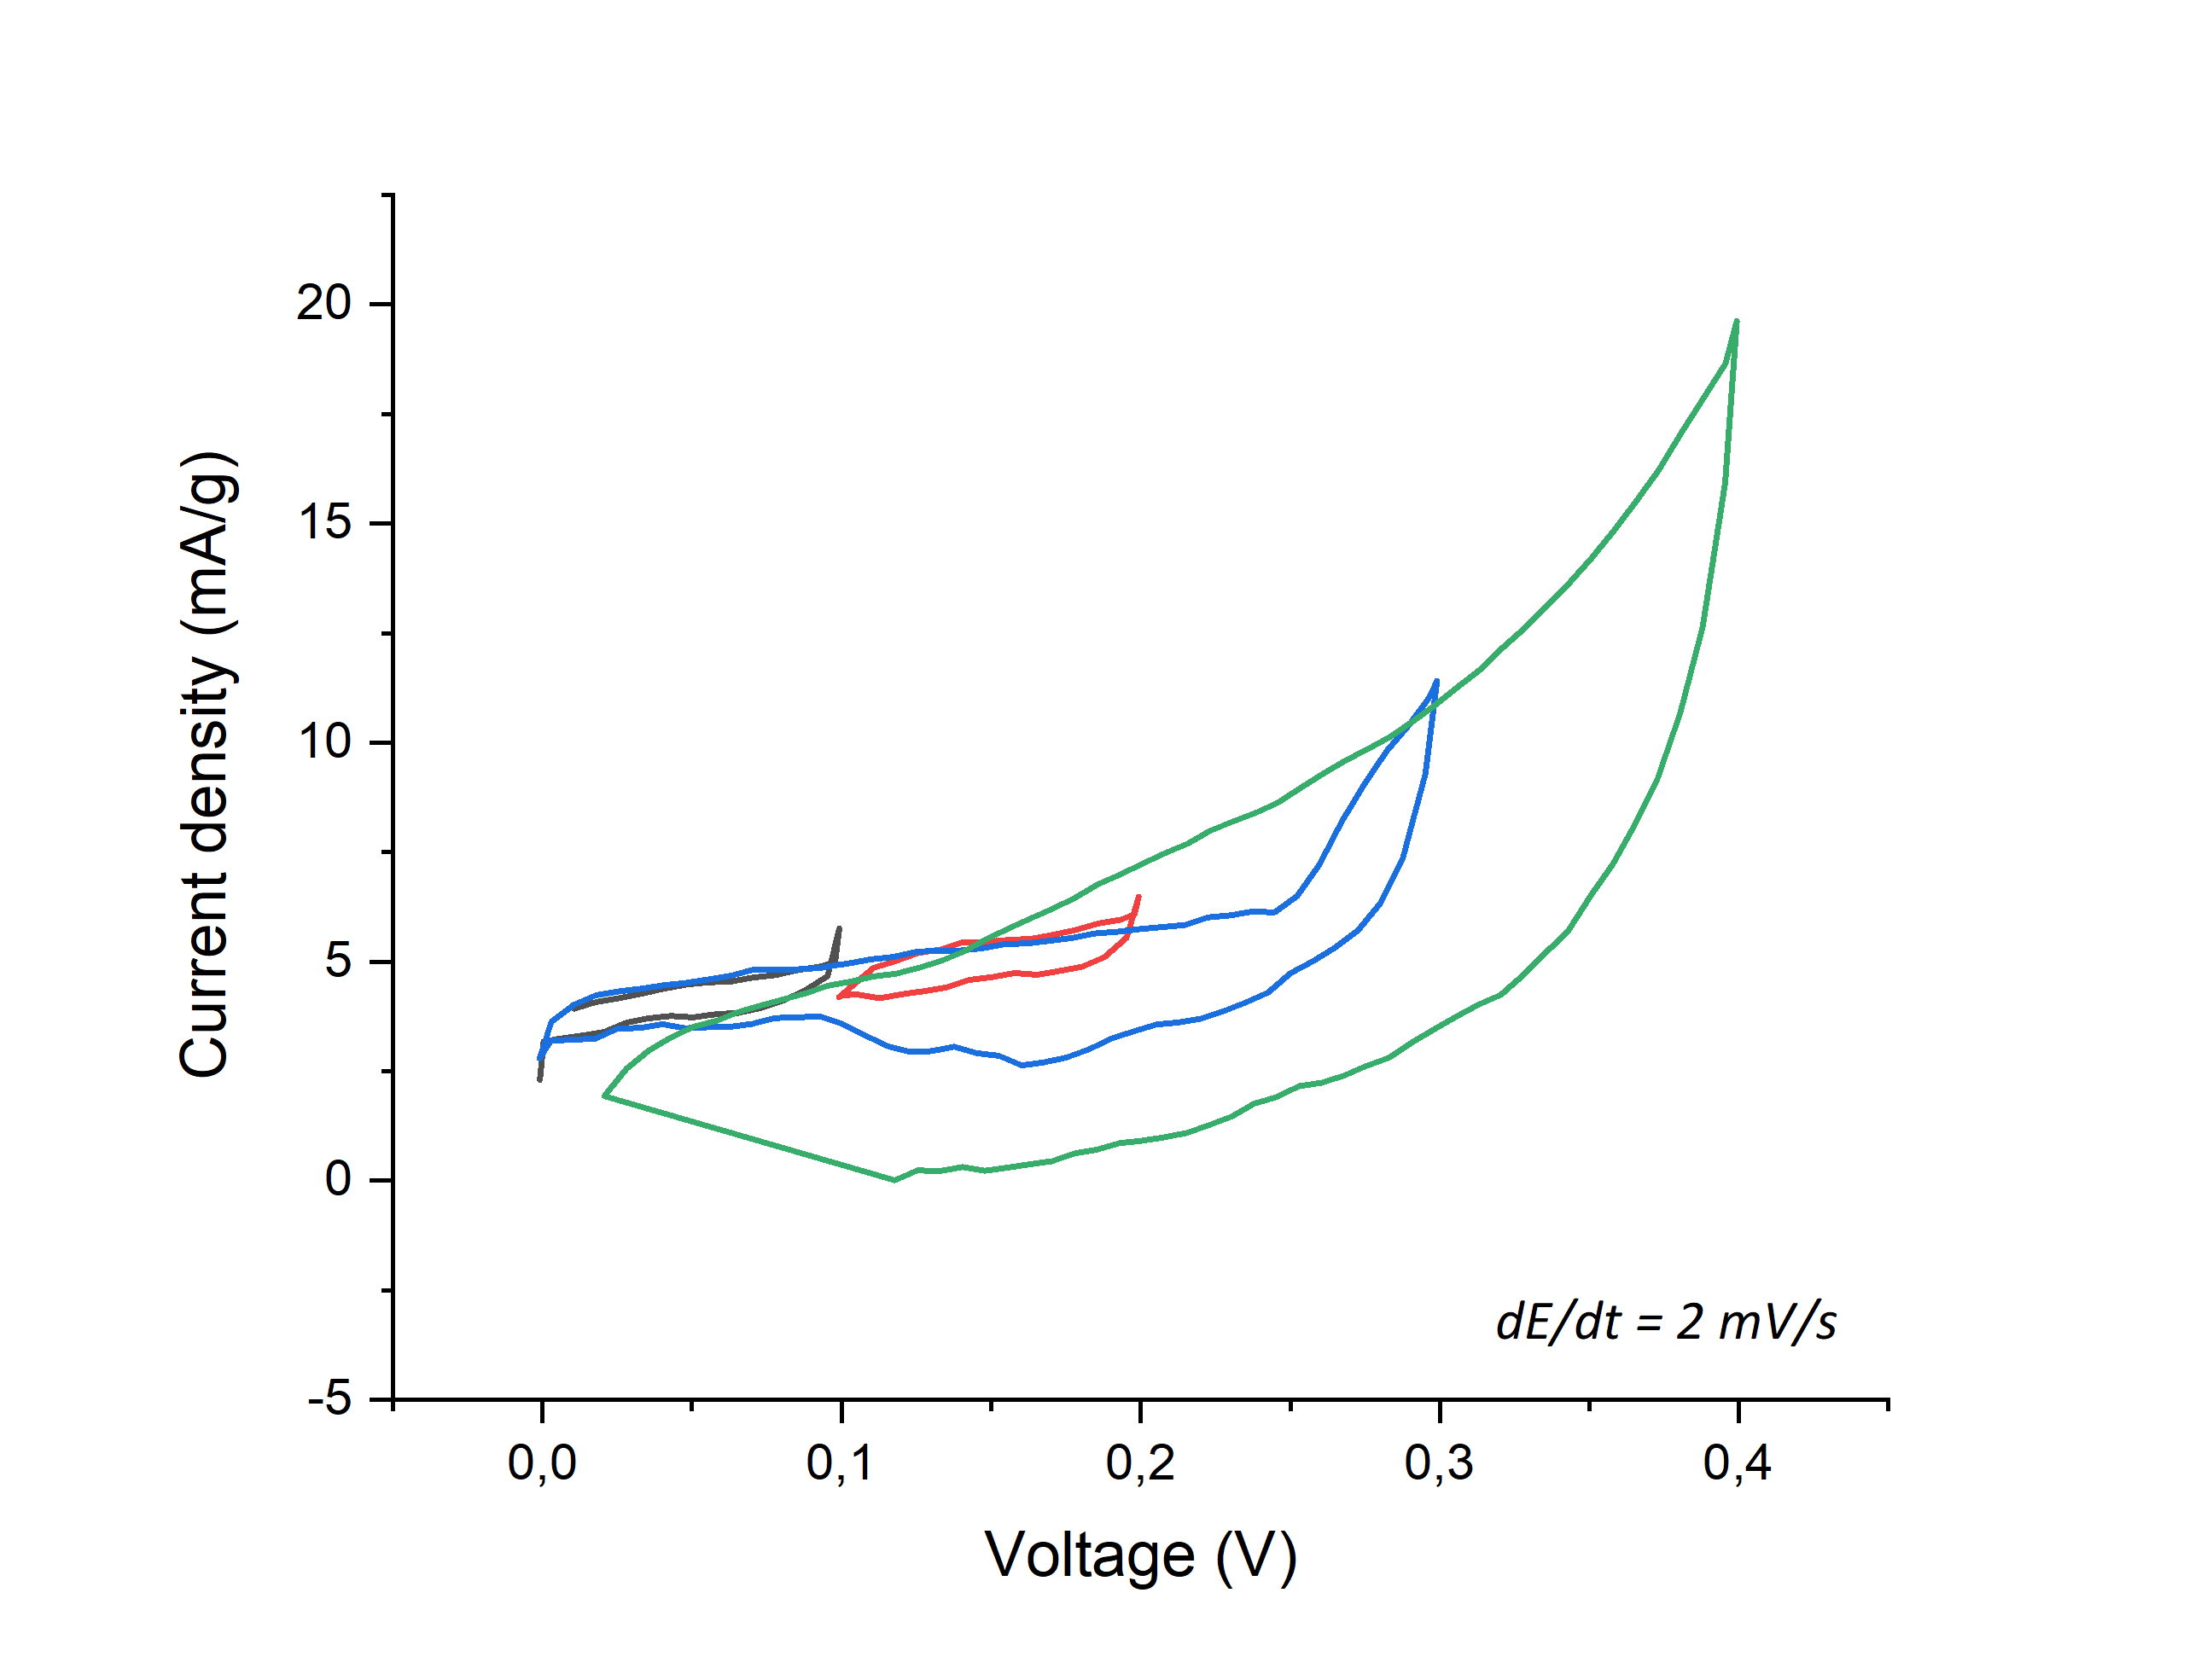
\includegraphics[width=1\textwidth]{Figures/Results/Electrochemistry/LIGF-MPU-NaNO3-Swagelok/Cell1/CV-all-voltages.jpg}
\captionsetup{width=0.9\linewidth}
\caption{LIGF-MPU Electrodes, Cell 1}
\label{fig:LIGF-MPU-cell1}
\end{subfigure}
\medskip
\caption{CV diagrams of LIGP-MPU and LIGF-MPU electrodes in Swagelok cells at various potential windows at a constant scan rate of 2\:mV/s}
\label{fig:LIG-MPU_CV}
\end{figure}

As can be seen from the figures above, neither of the cells show ideal rectangular shape in their CV curves. However the LIGP-MPU electrodes show somewhat better performance than the LIGF-MPU device. The inner area of the curves is larger for the LIGP which is directly related to the stored charge $Q$.

GCPL measurements have further confirmed a better, more stable, behaviour of the Type 4 LIGP-MPU electrodes. CC curves of these electrodes had well defined triangular shape with a minor iR drop. 

\begin{figure}[H]
\begin{subfigure}{0.49\textwidth}
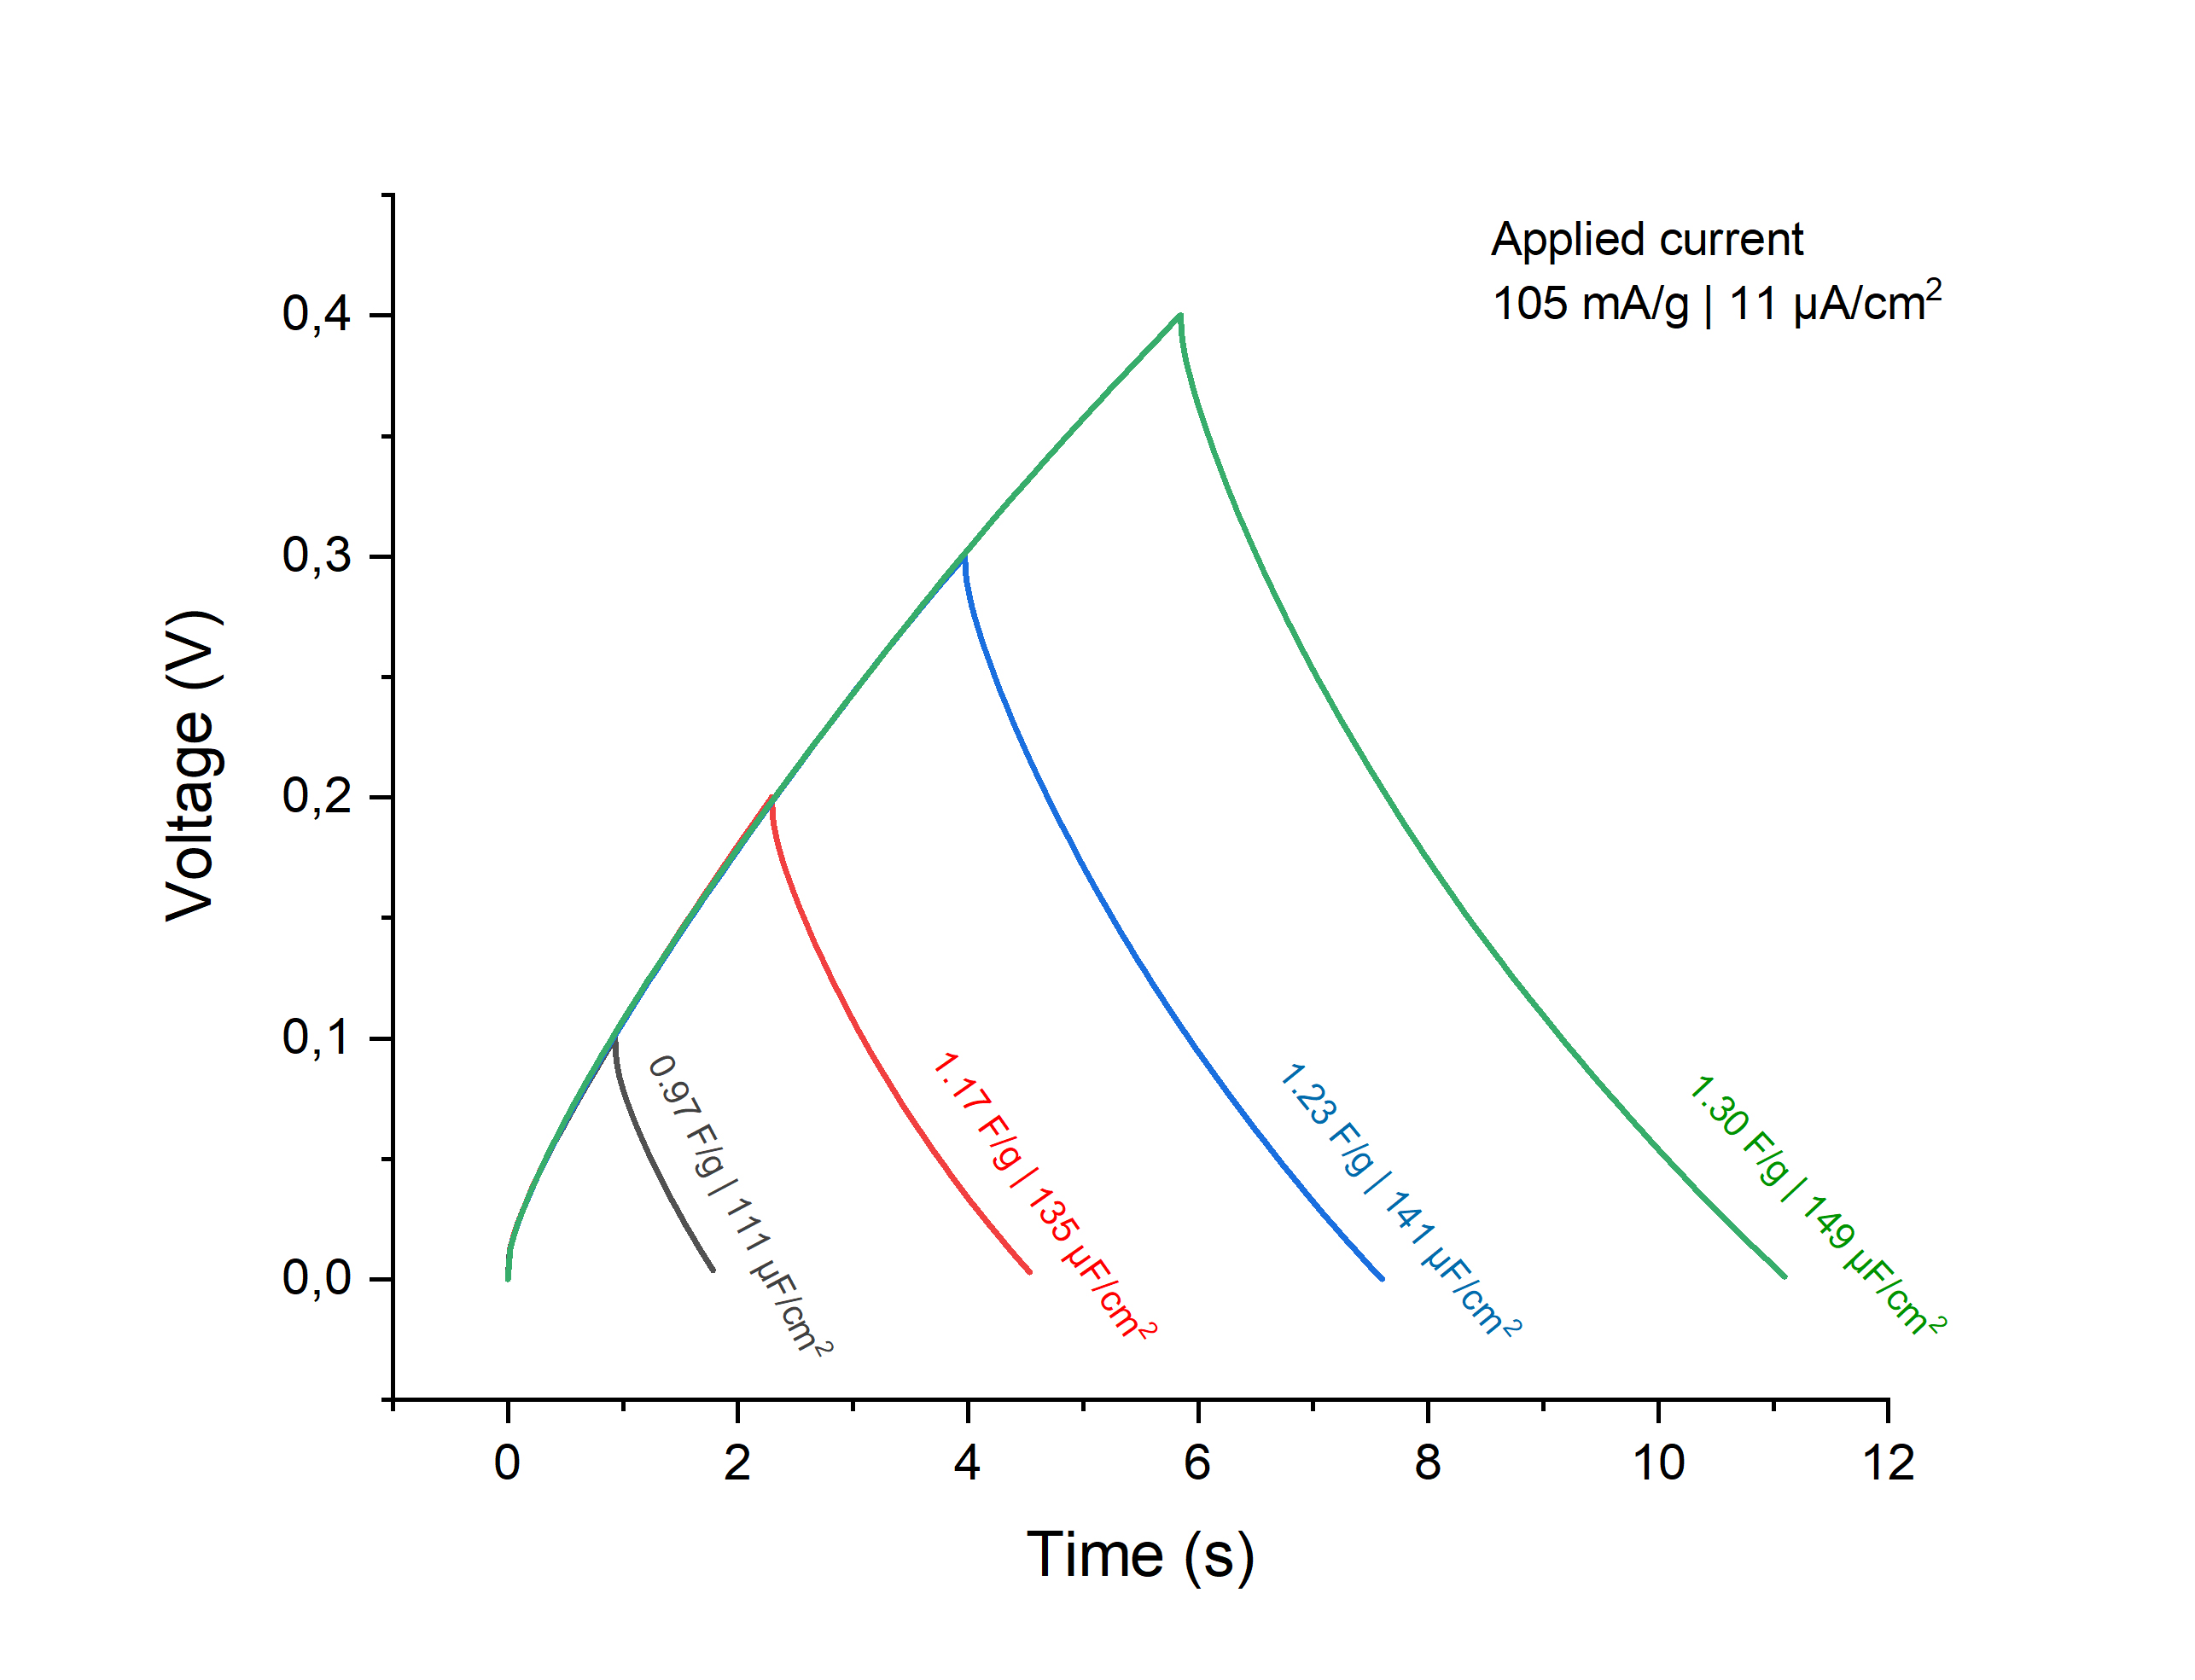
\includegraphics[width=1\textwidth]{Figures/Results/Electrochemistry/LIGP-MPU-NaNO3-Swagelok/Cell1/GCPL_130mA-g.jpg} 
\captionsetup{width=0.9\linewidth}
\caption{CC curves at various $V_{max}$}
\label{fig:LIGP-MPU-cell1-CC}
\end{subfigure}
\begin{subfigure}{0.49\textwidth}
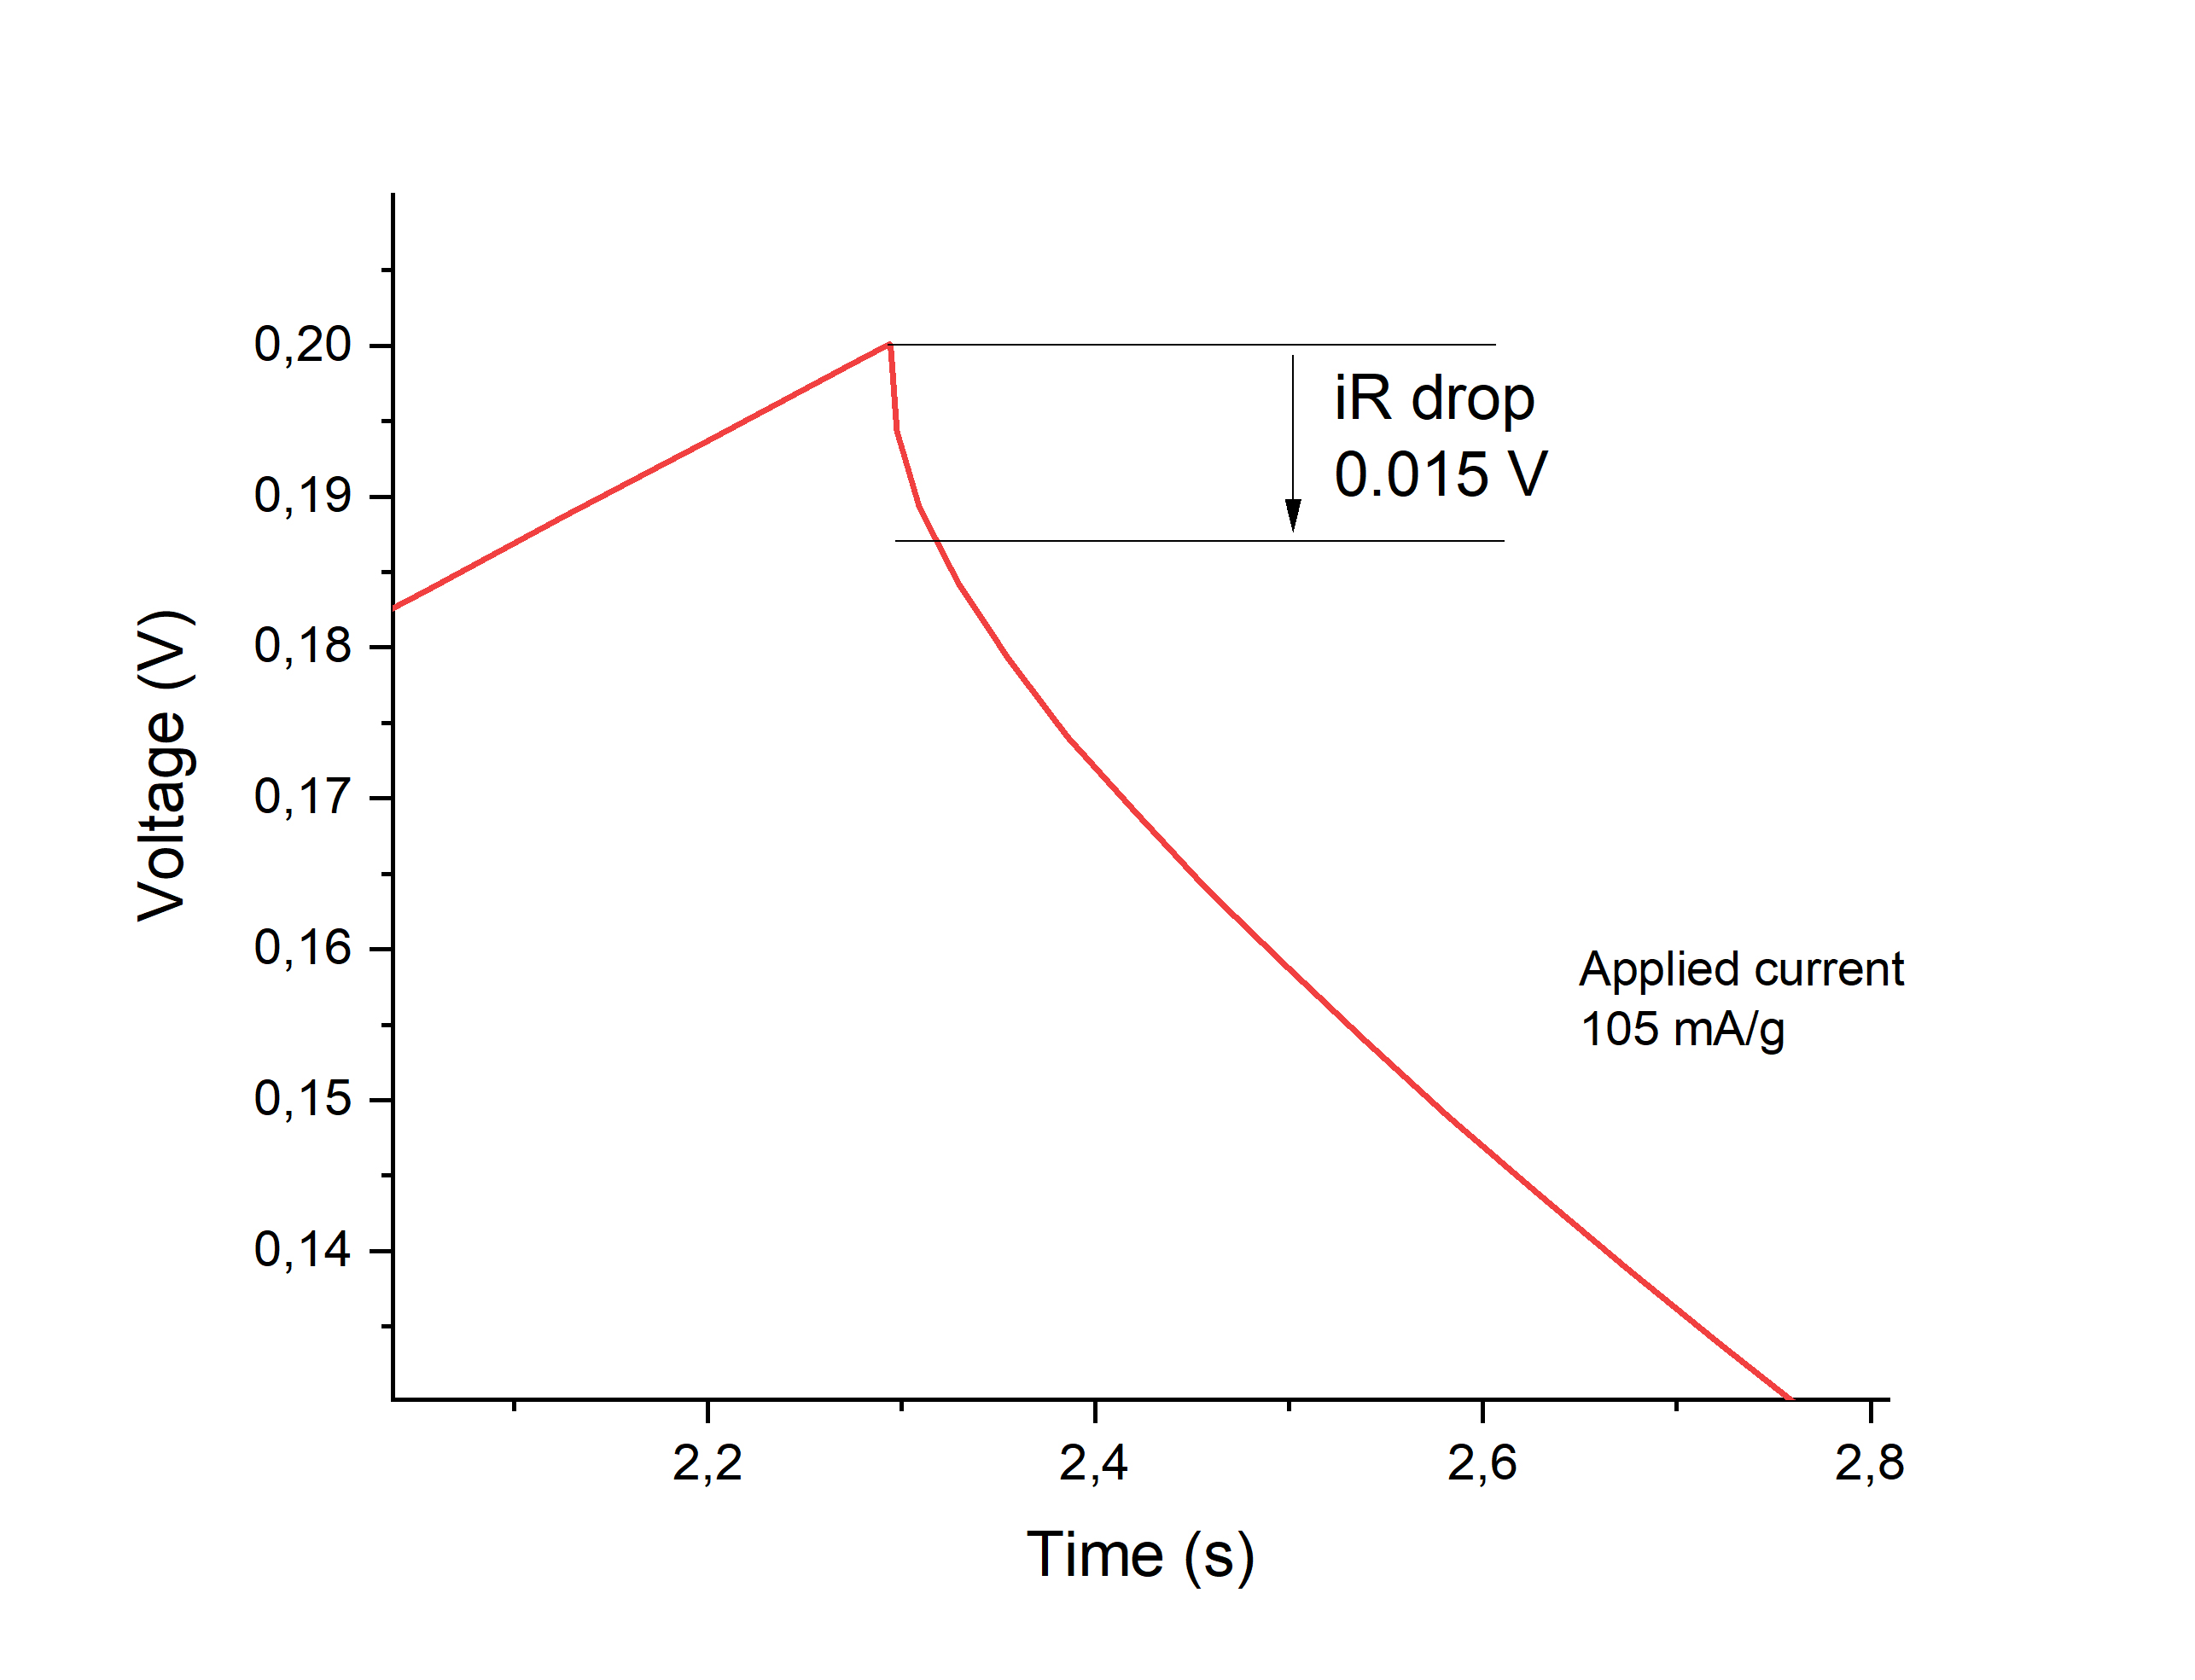
\includegraphics[width=1\textwidth]{Figures/Results/Electrochemistry/LIGP-MPU-NaNO3-Swagelok/Cell1/iR-drop.jpg}
\captionsetup{width=0.9\linewidth}
\caption{A minor iR drop of 0.015\:V of a CC curve}
\label{fig:LIGP-MPU-cell1-iR}
\end{subfigure}
\medskip
\caption{CC diagrams of LIGP-MPU electrodes in a Swagelok cell}
\label{fig:LIGP-MPU-CC}
\end{figure}

The LIGF-MPU electrodes have produced rather distorted charge-discharge $V(t)$ curves so that only the runs with $V_{max}$ of 0.1\:V and 0.2\:V had triangular appearance with relatively smaller iR drop than it was for the $V_{max}$ of 0.3\:V and 0.4\:V:

\begin{figure}[H]
\begin{subfigure}{0.49\textwidth}
\includegraphics[width=1\textwidth]{Figures/Results/Electrochemistry/LIGF-MPU-NaNO3-Swagelok/Cell1/GCPL-all-voltages.jpg} 
\captionsetup{width=0.9\linewidth}
\caption{CC curves at various $V_{max}$}
\label{fig:LIGF-MPU-cell1-CC}
\end{subfigure}
\begin{subfigure}{0.49\textwidth}
\includegraphics[width=1\textwidth]{Figures/Results/Electrochemistry/LIGF-MPU-NaNO3-Swagelok/Cell1/GCPL-low-voltages.jpg}
\captionsetup{width=0.9\linewidth}
\caption{Triangular CC curves at lower $V_{max}$}
\label{fig:LIGF-MPU-cell1-CC-2}
\end{subfigure}
\medskip
\caption{CC diagrams of LIGF-MPU electrodes in a Swagelok cell}
\label{fig:LIGF-MPU-CC}
\end{figure}

\textbf{Capacitance Evaluations for LIGP-MPU and LIGF-MPU Electrodes}

Capacitance evaluations for LIGP-MPU electrodes have shown relatively high capacitance values of around $1.2\div 2\:F/g$ which was comparable to the LIGP-Kapton Electrodes. Also there was a good consistency in numbers calculated from both types of electrochemical experiments. The trend which was previously seen for LIGP-Kapton electrodes, when capacitance grew proportionally to broadening of the CV weep window at the scan rate staying constant, could be seen in the case of these electrodes again. Similarly the capacitance values rose proportionally to $V_{max}$ for the CC data obtained with a non changing charge-discharge current. Figures \ref{fig:LIGP-MPU-cell1-C-CV-increase} and  \ref{fig:LIGP-MPU-cell1-C-CC-increase} provide comparison of the evaluated $C_g$ and $C_A$.

\begin{figure}[H]
\begin{subfigure}{0.49\textwidth}
\includegraphics[width=1\textwidth]{Figures/Results/Electrochemistry/LIGP-MPU-NaNO3-Swagelok/Cell1/Capac-Sweep.jpg} 
\captionsetup{width=0.9\linewidth}
\caption{Increase of specific capacitance with a $\Delta V$ increase at constant scan rate of 2\:mV/s}
\label{fig:LIGP-MPU-cell1-C-CV-increase}
\end{subfigure}
\begin{subfigure}{0.49\textwidth}
\includegraphics[width=1\textwidth]{Figures/Results/Electrochemistry/LIGP-MPU-NaNO3-Swagelok/Cell1/Capac-Vmax.jpg}
\captionsetup{width=0.9\linewidth}
\caption{Increase of specific capacitance with a rise of $V_{max}$ at a constant current of  105\:mA/s}
\label{fig:LIGP-MPU-cell1-C-CC-increase}
\end{subfigure}
\medskip
\caption{Specific Capacitance of LIGP-MPU electrode evaluated with CV and GCPL data}
\label{fig:LIGP-MPU-cell1-C-increase}
\end{figure}

As for the LIGF-MPU electrodes, the calculations have shown that $C_g$ values were about one order of magnitude lower than those for the LIGP-MPU electrodes (see Figure \ref{fig:LIGs-MPU-C-g}). 

For $C_A$, which evaluation does not take the mass of the active material into account but only the same for both types apparent surface area of the electrodes, the difference between LIGP and LIGF was not as dramatic although the overall character stayed similar showing better supercapacitor performance of the LIGP-MPU cell: 

\begin{figure}[H]
\begin{subfigure}{0.49\textwidth}
\includegraphics[width=1\textwidth]{Figures/Results/Electrochemistry/Comparisons/LIG-MPU-C_g.jpg} 
\captionsetup{width=0.9\linewidth}
\caption{Comparison of $C_g$ values for LIGP and LIGF on MPU electrodes}
\label{fig:LIGs-MPU-C-g}
\end{subfigure}
\begin{subfigure}{0.49\textwidth}
\includegraphics[width=1\textwidth]{Figures/Results/Electrochemistry/Comparisons/LIG-MPU-C_A.jpg}
\captionsetup{width=0.9\linewidth}
\caption{Comparison of $C_A$ values for LIGP and LIGF on MPU electrodes}
\label{fig:LIGs-MPU-C-A}
\end{subfigure}
\medskip
\caption{Specific Capacitance of LIG-MPU electrodes evaluated with GCPL data}
\label{fig:LIGs-MPU-C-Comparison}
\end{figure}


\textbf{Performance Comparison of LIG-based Electrodes in Swagelok Cells}

Electrochemical characterization of the SCs was performed for varying voltage ranges, however for all of the cells there was a common region of 0-0.2\:V where cyclic voltammetry was performed at different scan rates. To be able to compare the results obtained for the lowest scan rates were chosen to be a bench mark. Identically for the galvanostatic cycling with limited potential the capacitance values obtained for $V_max$ of 0.2 V at lowest charging-discharging current density were picked to be compared. The data was condensed into Table \ref{tab:swagelok-comparison}. As a remark, we would like to mention that these numbers were taken as the reference when making the further decisions concerning the combination of LIG/Substrate, which would be the most suitable for flexible soft applications. However, for the in-depth overview of the capacitance values and how they were derived, the reader is suggested to go through the data presented in the previous pages.

\begin{table}[H]
\centering
    \caption{Summary for Capacitance Values for Swagelok LIG(NaNO3, 1M) Cells}
    \label{tab:swagelok-comparison} 
\medskip
\medskip
\begin{tabular}{ l | l | l | l || l| l  } 
\hline
\multirow{2}{*}{Electrode}& \multirow{2}{*}{LIG Make} &
\multicolumn{2}{c||}{Cyclic Voltammetry} &
\multicolumn{2}{c}{GCPL} \\[13px]


	Type $\#$ &  & $C_g\:[F/g]$ & $C_A\:[F/g]$ & $C_g\:[F/g]$ & $C_A\:[F/g]$ \\ [13px]\hline
	
	1  & LIGP-Kapton$^{TM}$ & 1.87& 381 & 1.08  & 220 \\ [13px]
	
	2  & LIGF-Kapton$^{TM}$ & 0.19& 96 & 0.19 & 96 \\ [13px]
	
	3  & LIGF-PDMS-8:1 &0.04  & 21 & 0.04 & 19\\ [13px]
	
	4  & LIGP-MPU &1.20  & 138 & 1.17  & 135\\ [13px]
	
	5  & LIGF-MPU &0.19  & 51 & 0.14 & 38\\ [13px]
	
\end{tabular}
\end{table}


This cross comparison of the CV and GCPL data obtained for different Cells as it can be seen in Table \ref{tab:swagelok-comparison} allowed to make a few generalizations about the performance of LIGs on various substrates.

Firstly, it was found that all cells based on LIGP had significantly higher charge storage capability than LIGF-based electrodes. LIGP-cells have also shown better charge-discharge stability and less of the problems related to internal resistance.  Secondly, it can be also seen that the LIGF-PDMS composite have shown the worst performance among all, which could be addressed to an overall poor capacitance of LIGF aggravated by the fact it was to a big part embedded into the dielectric matrix of polydimethylsiloxane. Figure \ref{fig:LIGF-cells-C_g} provides the visual comparison chart underlining these two observations.

Further it is important to make a point concerning the two approaches which were used to evaluate the values of specific capacitance. The common way to asses the supercapacitor performance by comparing $C_A$ values of the electrodes makes it difficult to estimate a real change in performance when talking about very light materials used as an active layer. Indeed in our case the mass of LIGP on Kapton was 0.16\:mg. whereas the its mass on MPU was only 0.09\:mg, which inevitably introduces a difference by the factor of 0.16/0.09 into specific gravimetric capacitance all other parameters being equal. In contrary, the specific areal capacitance would not change in these circumstances, which apparently makes it difficult to compare material properties when they lay as the central staged question of the investigation. Graph in Figure \ref{fig:Cg-vs-Ca} demonstrates on the example of data obtained in this work that discrepancy in $C_g\:vs.\:C_A$ trend for the situations when the mass of the electrode material changes without a change in the total geometrical area of the electrode.  

\begin{figure}[H]
\centering
\includegraphics[width=0.8\textwidth]{Figures/Results/Electrochemistry/Comparisons/Gr-Capacitance-vs-Current.jpg}
\medskip
\captionsetup{width=1\linewidth}
\caption{Comparison of $C_g$ values of LIGF and LIGP based cells}
\label{fig:LIGF-cells-C_g}
\end{figure}

 When comparing LIGP-MPU and LIGP-PI cells from Figure \ref{fig:Cg-vs-Ca} one can see the 230$\%$ change in specific areal capacitance, whereas the  specific gravimetric capacitance changes only by 130$\%$.

\begin{figure}[H]
\begin{subfigure}{0.49\textwidth}
\includegraphics[width=1\textwidth]{Figures/Results/Electrochemistry/Comparisons/Gravimetric-vs-Areal-Capacitance-Change.jpg}
\medskip
\captionsetup{width=0.9\linewidth}
\caption{Comparison of $C_g$ and $C_A$ trends for cells with varying mass $m$ of an active material when electrode surface area $s$ stays constant}
\label{fig:Cg-vs-Ca}
\end{subfigure}
\begin{subfigure}{0.49\textwidth}
\includegraphics[width=1\textwidth]{Figures/Results/Electrochemistry/Comparisons/Gravim-Cap-CV-GCPL.jpg}
\medskip
\captionsetup{width=0.9\linewidth}
\caption{Comparison of $C_g$ values and trends obtained from CV and from GCPL data}
\label{fig:CV-vs-GCPL-final}
\end{subfigure}
\medskip
\caption{Specific Capacitance of LIG-MPU electrodes evaluated with GCPL data}
\label{fig:Capacitances-discuss}
\end{figure}


One more point which needs to be brought to discussion is the consistency between the CV and GCPL data. On the example of our data shown in Figure \ref{fig:CV-vs-GCPL-final} it can be seen, that except one point the values and their trends estimated with these two technique lay in a qualitative agreement with each other. However not all the measurements gave quantitatively the same numbers, which however is caused by the fact that the electrical settings at which the cells were tested cannot be assumed to be absolutely identical.



XXX Energy and power densities.





 
 %The capacitance was also calculated for the same charge-discharge rates using the classical equation below:  
 %(page 4 from the tutorial)
 
 %Where Ich/disch is the charge or discharge current and abs (slope Ewe vs. t) is the absolute value of the slope of Ewe vs. time 
 



\subsection{Impedance Spectroscopy}

Mummy... it never ends

\section{Discussion on Biocompatibility}